\documentclass[final]{our-book}
% %% Partial processing for IA1
% \includeonly{preface,introduction,holLogic,c2conops,pki}



%%%%%%%%%%%


\usepackage{makeidx}
% \usepackage{index}
\usepackage{our-multind}

\usepackage{times, mathptm}
\usepackage{sunil}
\usepackage{amsmath}
% \usepackage{times,amsmath}
\usepackage[thmmarks,amsmath]{ntheorem}
%\usepackage{multicol}
\usepackage{apalike}
\usepackage{xspace}
\usepackage{pifont}
\usepackage{float}
\floatstyle{ruled}
\restylefloat{figure}

\usepackage{array}
\usepackage{delarray}

\usepackage{fancybox}
%% the following two packages are needed to properly annotate exercises 
%% on both odd and even pages
\usepackage{mparhack}
\usepackage{chngpage}  

%% the following packages are for source code listings
\usepackage{listings}
\usepackage{textcomp}

% %% the following for simulating typed text
% \usepackage{fancyvrb}

%\includeonly{introduction}
%\includeonly{networkedAC}
%\includeonly{coreRules,basicACconcepts}


%% Added 5 Nov 2004
%%
%% The following code will enable both LaTeX (and dvips) and PDF LaTeX
%% to work on the same files, making both our lives much happier.
%%
\ifx\pdfoutput\undefined
\usepackage[dvips]{graphicx}
\else
\usepackage[pdftex]{graphicx}
\usepackage{epstopdf}
\pdfcompresslevel=9
\fi
% if using pdflatex, we must use our .pdf images instead of .(e?)ps
\ifx\pdfoutput\undefined
\else
\DeclareGraphicsExtensions{.pdf,.gif,.jpg} % the formats we have images in
\fi

%\usepackage[dvipsnames,usenames]{color}
\usepackage[svgnames]{xcolor}

%% for colored text
\newcommand{\redtext}[1]{\textcolor{red}{#1}}
\newcommand{\bluetext}[1]{\textcolor{blue}{#1}}
\newcommand{\cyantext}[1]{\textcolor{cyan}{#1}}
\newcommand{\magtext}[1]{\textcolor{magenta}{#1}}
\newcommand{\greentext}[1]{\textcolor{green}{#1}}
\newcommand{\tealtext}[1]{\textcolor{teal}{#1}}
\newcommand{\olivetext}[1]{\textcolor{olive}{#1}}
\newcommand{\standout}[1]{\textcolor{orange}{#1}}

\newcommand{\seq}[2]{\ensuremath{\set{#1} \vdash {#2}}}
\newcommand{\seqs}[2]{\ensuremath{#1 \vdash {#2}}}
\newcommand{\sq}[1]{\ensuremath{\vdash {#1}}}

\newcommand{\goal}[2]{\ensuremath{\set{#1}\;\text{ ?-- }\;{#2}}}
\newcommand{\goals}[2]{\ensuremath{{#1}\;\text{ ?-- }\;{#2}}}
\newcommand{\gls}[1]{\ensuremath{\text{ ?-- }\;{#1}}}

% \renewcommand{\irule}[3]
%     {\ensuremath{{\displaystyle \frac{#1}{#2}}\quad \infname{#3}}}
\newcommand{\tac}[3]{
  \ensuremath{\begin{tabular}{c}
    {#1}\\\hline\hline{#2}
  \end{tabular}\quad}{#3}}


%\usepackage{fancyheadings}
\usepackage{amssymb, amsmath}
\usepackage{enumerate}

% \usepackage{float}
% %\floatstyle{ruled}
% \floatstyle{boxed}
% \restylefloat{figure}
% \restylefloat{table}


% %\usepackage{theorem}

%% get parts to show up correctly in the table of contents
\makeatletter

\let\toc@draw\relax
\def\l@part#1#2{%
 \toc@draw
 \gdef\toc@draw{\draw@part{\large #1}{\large #2}}}

%% following looks like \draw@chapter from sunil.sty
%% only change was in vertical spacing, which is sufficient
%% to prevent bad page break in toc
\def\draw@part#1#2{%
 \addpenalty{-\@highpenalty}%
    \addvspace{2.25em \@plus\p@}%
%  \vskip1em plus\p@
  \@tempdima1.5em
  \begingroup
    \parindent\z@\rightskip\@pnumwidth
    \parfillskip-\rightskip
    \bfseries
    \leavevmode
    \advance\leftskip\@tempdima
    \hskip-\leftskip
    {#1\hfil}\nobreak
      \if@pdf
      \else
        \hfil\nobreak\hb@xt@\@pnumwidth{\hss #2}%
\fi
    \par
    {\it\draw@authors}%
    \penalty\@highpenalty\endgroup}

\makeatother
%%%%%%%%%%%%%%%%%

\newtheorem{master}{Master}[section]
{%\theoremsymbol{\rule{.7ex}{1.8ex}}
  \theoremsymbol{\ensuremath{\Diamond}}
  \theoremstyle{break}
  \theoremheaderfont{\bfseries\slshape}
  \theorembodyfont{\upshape}
  \theoremprework{\bigskip}
  \theorempostwork{\bigskip}
%  \theoremindent1em
  \newtheorem{examp}{Example}[chapter]
}

{  
  \theorembodyfont{\itshape}
  {
    \theoremsymbol{\rule{.7ex}{.7ex}}
    \newtheorem{defin}{Definition}[chapter]
  }
  \newtheorem{thmexercise}{Exercise}[section]  
}

%  \theoremprework{\bigskip}



%----the environment for labeled exercises---------------------


\newcommand{\appn}{\ding{46}}
\newcommand{\analysis}{
\includegraphics[width=1.5em]{Figures/exerciseLabels/mag-glass}} 
\newcommand{\synthesis}{
\includegraphics[width=1.5em]{Figures/exerciseLabels/hammer}} 
\newcommand{\eval}{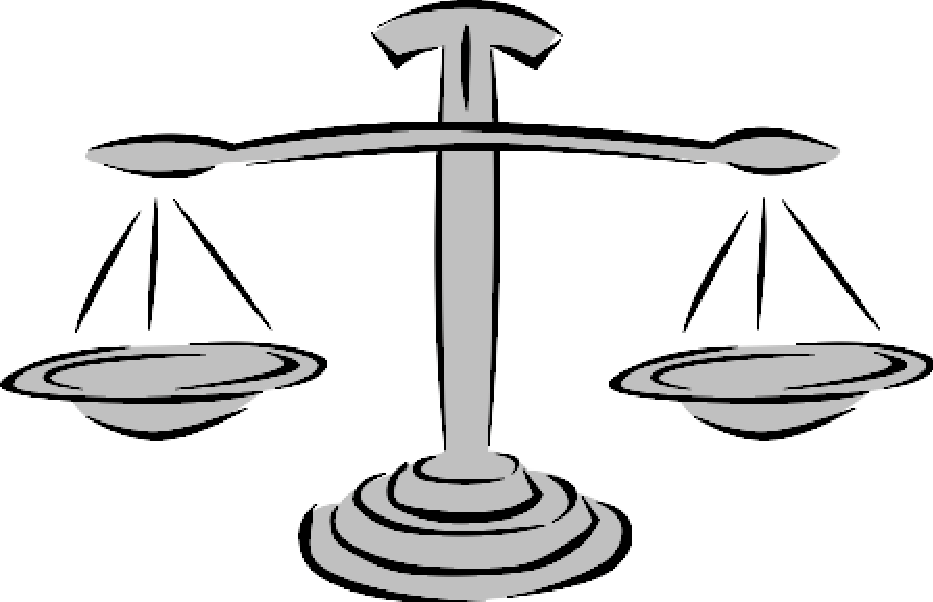
\includegraphics[width=1.5em]{Figures/exerciseLabels/scales}} 

\renewenvironment{definition}{\begin{defin}}{\end{defin}}
\renewenvironment{example}{\begin{examp}}{\end{examp}}
\newenvironment{exercise}[1][\appn]{\begin{thmexercise}\ %
    \checkoddpage
    \ifcpoddpage \reversemarginpar \fi
    \marginpar{\hfill #1}%
    \renewcommand{\theenumi}{\alph{enumi}}%
}
{\renewcommand{\theenumi}{\roman{enumi}}%
 \end{thmexercise}}


\newcommand{\sue}[1]{\textbf{\textsf{#1}}}
\newcommand{\suebox}[1]{%
  \fbox{\parbox[t]{4.5in}{\textsc{Note to Self:} 
      \begin{center}
        \ \\ #1 \ \\ \ 
      \end{center}}}}

\newcommand{\chinbox}[1]{%
  \fbox{\parbox[t]{4.5in}{\textsc{Note to Self:} 
      \begin{center}
        #1
      \end{center}}}}

%% counters for use in pki.tex
%% had to be added here to allow piecemeal compilation of book.tex
\newcounter{count} \newcounter{restart} 

%%===Index related commands=====
%% main index
\newcommand{\mainindex}[1]{\index{book}{#1}}
%% symbol index
\newcommand{\symindex}[1]{\index{symbol}{#1}}

%% create the index
% \makeindex
\makeindex{symbol}
\makeindex{book}



% %%----------
% %% HOL stuff
% %%----------

% =====================================================================
%
% Macros for typesetting the HOL system manual
%
% =====================================================================

% ---------------------------------------------------------------------
% Abbreviations for words and phrases
% ---------------------------------------------------------------------

\newcommand\TUTORIAL{{\footnotesize\sl TUTORIAL}}
\newcommand\DESCRIPTION{{\footnotesize\sl DESCRIPTION}}
\newcommand\REFERENCE{{\footnotesize\sl REFERENCE}}
\newcommand\LOGIC{{\footnotesize\sl LOGIC}}
\newcommand\LIBRARIES{{\footnotesize\sl LIBRARIES}}

\newcommand{\bs}{\texttt{\char'134}} % backslash
\newcommand{\lb}{\texttt{\char'173}} % left brace
\newcommand{\rb}{\texttt{\char'175}} % right brace
\newcommand{\td}{\texttt{\char'176}} % tilde
\newcommand{\lt}{\texttt{\char'74}} % less than
\newcommand{\gt}{\texttt{\char'76}} % greater than
\newcommand{\dol}{\texttt{\char'44}} % dollar
% double back quotes ``
\newcommand{\dq}{\texttt{\char'140\char'140}}
%These macros were included by slind:

\newcommand{\holquote}[1]{\dq#1\dq}

\def\HOL{{\small HOL}}
\def\holn{\HOL}  % i.e. hol n(inety-eight), no digits in
                 % macro names is a bit of a pain; deciding to do away
                 % with hol98 nomenclature means that we just want to
                 % write HOL for hol98.
\def\holnversion{Kananaskis-7}
\def\holnsversion{Kananaskis~7} % version with space rather than hyphen
\def\LCF{{\small LCF}}
\def\LCFLSM{{\small LCF{\kern-.2em}{\normalsize\_}{\kern0.1em}LSM}}
\def\PPL{{\small PP}{\kern-.095em}$\lambda$}
\def\PPLAMBDA{{\small PPLAMBDA}}
\def\ML{{\small ML}}
\def\holmake{\texttt{Holmake}}

\newcommand\ie{\mbox{i{.}e{.}}}
\newcommand\eg{\mbox{e{.}g{.}}}
\newcommand\viz{\mbox{viz{.}}}
\newcommand\adhoc{\mbox{\it ad hoc}}
\newcommand\etal{{\it et al.\/}}
\newcommand\etc{\mbox{etc{.}}}

% ---------------------------------------------------------------------
% Simple abbreviations and macros for mathematical typesetting
% ---------------------------------------------------------------------

\newcommand\fun{{\to}}
\newcommand\prd{{\times}}

\newcommand\conj{\ \wedge\ }
\newcommand\disj{\ \vee\ }
\newcommand\imp{ \Rightarrow }
\newcommand\eqv{\ \equiv\ }
\newcommand\cond{\rightarrow}
\newcommand\vbar{\mid}
\newcommand\turn{\ \vdash\ }
\newcommand\hilbert{\varepsilon}
\newcommand\eqdef{\ \equiv\ }

\newcommand\natnums{\mbox{${\sf N}\!\!\!\!{\sf N}$}}
\newcommand\bools{\mbox{${\sf T}\!\!\!\!{\sf T}$}}

\newcommand\p{$\prime$}
\newcommand\f{$\forall$\ }
\newcommand\e{$\exists$\ }

% \newcommand\orr{$\vee$\ }
\newcommand\negg{$\neg$\ }

\newcommand\arrr{$\rightarrow$}
\newcommand\hex{$\sharp $}

\newcommand{\uquant}[1]{\forall #1.\ }
\newcommand{\equant}[1]{\exists #1.\ }
\newcommand{\hquant}[1]{\hilbert #1.\ }
\newcommand{\iquant}[1]{\exists ! #1.\ }
\newcommand{\lquant}[1]{\lambda #1.\ }

\newcommand{\leave}[1]{\\[#1]\noindent}
\newcommand\entails{\mbox{\rule{.3mm}{4mm}\rule[2mm]{.2in}{.3mm}}}

% ---------------------------------------------------------------------
% Font-changing commands
% ---------------------------------------------------------------------

\newcommand{\theory}[1]{\hbox{{\small\tt #1}}}
\newcommand{\theoryimp}[1]{\texttt{#1}}

\newcommand{\con}[1]{{\sf #1}}
\newcommand{\rul}[1]{{\tt #1}}
\newcommand{\ty}[1]{\textsl{#1}}

\newcommand{\ml}[1]{\mbox{{\def\_{\char'137}\texttt{#1}}}}
\newcommand{\holtxt}[1]{\ml{#1}}
\newcommand\ms{\tt}
\newcommand{\s}[1]{{\small #1}}

\newcommand{\pin}[1]{{\bf #1}}
\def\m#1{\mbox{\normalsize$#1$}}

% ---------------------------------------------------------------------
% Abbreviations for particular mathematical constants etc.
% ---------------------------------------------------------------------

\newcommand\T{\con{T}}
\newcommand\F{\con{F}}
\newcommand\OneOne{\con{One\_One}}
\newcommand\OntoSubset{\con{Onto\_Subset}}
\newcommand\Onto{\con{Onto}}
\newcommand\TyDef{\con{Type\_Definition}}
\newcommand\Inv{\con{Inv}}
\newcommand\com{\con{o}}
\newcommand\Id{\con{I}}
\newcommand\MkPair{\con{Mk\_Pair}}
\newcommand\IsPair{\con{Is\_Pair}}
\newcommand\Fst{\con{Fst}}
\newcommand\Snd{\con{Snd}}
\newcommand\Suc{\con{Suc}}
\newcommand\Nil{\con{Nil}}
\newcommand\Cons{\con{Cons}}
\newcommand\Hd{\con{Hd}}
\newcommand\Tl{\con{Tl}}
\newcommand\Null{\con{Null}}
\newcommand\ListPrimRec{\con{List\_Prim\_Rec}}


\newcommand\SimpRec{\con{Simp\_Rec}}
\newcommand\SimpRecRel{\con{Simp\_Rec\_Rel}}
\newcommand\SimpRecFun{\con{Simp\_Rec\_Fun}}
\newcommand\PrimRec{\con{Prim\_Rec}}
\newcommand\PrimRecRel{\con{Prim\_Rec\_Rel}}
\newcommand\PrimRecFun{\con{Prim\_Rec\_Fun}}

\newcommand\bool{\ty{bool}}
\newcommand\num{\ty{num}}
\newcommand\ind{\ty{ind}}
\newcommand\lst{\ty{list}}

% ---------------------------------------------------------------------
% \minipagewidth = \textwidth minus 1.02 em
% ---------------------------------------------------------------------

\newlength{\minipagewidth}
\setlength{\minipagewidth}{\textwidth}
\addtolength{\minipagewidth}{-1.02em}

% ---------------------------------------------------------------------
% Environment for the items on the title page of a case study
% ---------------------------------------------------------------------

\newenvironment{inset}[1]{\noindent{\large\bf #1}\begin{list}%
{}{\setlength{\leftmargin}{\parindent}%
\setlength{\topsep}{-.1in}}\item }{\end{list}\vskip .4in}

% ---------------------------------------------------------------------
% Macros for little HOL sessions displayed in boxes.
%
% Usage: (1) \setcounter{sessioncount}{1} resets the session counter
%
%        (2) \begin{session}\begin{verbatim}
%             .
%              < lines from hol session >
%             .
%            \end{verbatim}\end{session}
%
%            typesets the session in a numbered box.
% ---------------------------------------------------------------------

\newlength{\hsbw}
\setlength{\hsbw}{\textwidth}
\addtolength{\hsbw}{-\arrayrulewidth}
\addtolength{\hsbw}{-\tabcolsep}
\newcommand\HOLSpacing{13pt}

\newcounter{sessioncount}
\setcounter{sessioncount}{0}

\newenvironment{session}{\begin{flushleft}
 \refstepcounter{sessioncount}
 \begin{tabular}{@{}|c@{}|@{}}\hline
 \begin{minipage}[b]{\hsbw}
 \vspace*{-.5pt}
 \begin{flushright}
 \rule{0.01in}{.15in}\rule{0.3in}{0.01in}\hspace{-0.35in}
 \raisebox{0.04in}{\makebox[0.3in][c]{\footnotesize\sl \thesessioncount}}
 \end{flushright}
 \vspace*{-.55in}
 \begingroup\small\baselineskip\HOLSpacing}{\endgroup\end{minipage}\\ \hline
 \end{tabular}
 \end{flushleft}}

% ---------------------------------------------------------------------
% Macro for boxed ML functions, etc.
%
% Usage: (1) \begin{holboxed}\begin{verbatim}
%               .
%               < lines giving names and types of mk functions >
%               .
%            \end{verbatim}\end{holboxed}
%
%            typesets the given lines in a box.
%
%            Conventions: lines are left-aligned under the "g" of begin,
%            and used to highlight primary reference for the ml function(s)
%            that appear in the box.
% ---------------------------------------------------------------------

\newenvironment{holboxed}{\begin{flushleft}
  \begin{tabular}{@{}|c@{}|@{}}\hline
  \begin{minipage}[b]{\hsbw}
% \vspace*{-.55in}
  \vspace*{.06in}
  \begingroup\small\baselineskip\HOLSpacing}{\endgroup\end{minipage}\\ \hline
  \end{tabular}
  \end{flushleft}}

% ---------------------------------------------------------------------
% Macro for unboxed ML functions, etc.
%
% Usage: (1) \begin{hol}\begin{verbatim}
%               .
%               < lines giving names and types of mk functions >
%               .
%            \end{verbatim}\end{hol}
%
%            typesets the given lines exactly like {boxed}, except there's
%            no box.
%
%            Conventions: lines are left-aligned under the "g" of begin,
%            and used to display ML code in verbatim, left aligned.
% ---------------------------------------------------------------------

\newenvironment{hol}{\begin{flushleft}
 \begin{tabular}{c@{}@{}}
 \begin{minipage}[b]{\hsbw}
% \vspace*{-.55in}
 \vspace*{.06in}
 \begingroup\small\baselineskip\HOLSpacing}{\endgroup\end{minipage}\\
 \end{tabular}
 \end{flushleft}}

% ---------------------------------------------------------------------
% Emphatic brackets
% ---------------------------------------------------------------------

\newcommand\leb{\lbrack\!\lbrack}
\newcommand\reb{\rbrack\!\rbrack}


% ---------------------------------------------------------------------
% Quotations
% ---------------------------------------------------------------------


%These macros were included by ap; they are used in Chapters 9 and 10
%of the HOL DESCRIPTION

\newcommand{\inds}%standard infinite set
 {\mbox{\rm I}}

\newcommand{\ch}%standard choice function
 {\mbox{\rm ch}}

\newcommand{\den}[1]%denotational brackets
 {[\![#1]\!]}

\newcommand{\two}%standard 2-element set
 {\mbox{\rm 2}}

% %macros for pictures in latex

\def\puthrule(#1,#2)#3{\put(#1,#2){\line(1,0){#3}}}
\def\putvrule(#1,#2)#3{\put(#1,#2){\line(0,1){#3}}}
\def\putdot(#1){\put(#1){\circle*{0.2}}}
\def\ignore#1{}
\def\putgrid(#1,#2)(#3,#4){\multiput(#1,#2)(1,0){#3}{\circle*{0.2}}
\multiput(#1,#2)(0,1){#4}{\circle*{0.2}}}

\def\putdevice(#1,#2)#3{\put(#1,#2){\framebox(4,2){\small{\tt #3}}}}
\def\putport(#1,#2)#3{\put(#1,#2){\makebox(4,1){\small{\tt #3}}}}


% =====================================================================
% Macros for typesetting hol reference manual entries
% =====================================================================

% ---------------------------------------------------------------------
% boolean flag for verbose printing of reference manual typesetting
% ---------------------------------------------------------------------

\newif\ifverboseref
\verbosereffalse                          % don't be verbose

% ---------------------------------------------------------------------
% Macro for generating right-hand page running titles.
% ---------------------------------------------------------------------

\makeatletter

\def\mkhead{\futurelet\@t\chsize}
\def\chsize#1.{\ifx a\@t \markright{{\protect\bf #1}}\else
               \ifx b\@t \markright{{\protect\bf #1}}\else
               \ifx c\@t \markright{{\protect\bf #1}}\else
               \ifx d\@t \markright{{\protect\bf #1}}\else
               \ifx e\@t \markright{{\protect\bf #1}}\else
               \ifx f\@t \markright{{\protect\bf #1}}\else
               \ifx g\@t \markright{{\protect\bf #1}}\else
               \ifx h\@t \markright{{\protect\bf #1}}\else
               \ifx i\@t \markright{{\protect\bf #1}}\else
               \ifx j\@t \markright{{\protect\bf #1}}\else
               \ifx k\@t \markright{{\protect\bf #1}}\else
               \ifx l\@t \markright{{\protect\bf #1}}\else
               \ifx m\@t \markright{{\protect\bf #1}}\else
               \ifx n\@t \markright{{\protect\bf #1}}\else
               \ifx o\@t \markright{{\protect\bf #1}}\else
               \ifx p\@t \markright{{\protect\bf #1}}\else
               \ifx q\@t \markright{{\protect\bf #1}}\else
               \ifx r\@t \markright{{\protect\bf #1}}\else
               \ifx s\@t \markright{{\protect\bf #1}}\else
               \ifx t\@t \markright{{\protect\bf #1}}\else
               \ifx u\@t \markright{{\protect\bf #1}}\else
               \ifx v\@t \markright{{\protect\bf #1}}\else
               \ifx w\@t \markright{{\protect\bf #1}}\else
               \ifx z\@t \markright{{\protect\bf #1}}\else
               \ifx y\@t \markright{{\protect\bf #1}}\else
               \ifx z\@t \markright{{\protect\bf #1}}\else
               \markright{{\protect\small\bf #1}}\fi
               \fi\fi\fi\fi\fi\fi\fi\fi\fi\fi\fi\fi\fi\fi\fi
               \fi\fi\fi\fi\fi\fi\fi\fi\fi\fi}

\makeatother

% ---------------------------------------------------------------------
% \DOC{<object>}  : start a manual entry for <object>.
% ---------------------------------------------------------------------

\newcommand{\DOC}[2]%
{\bigskip
 {\ifverboseref{\def\_{\string_}\typeout{Typesetting: #1}}\fi}
 \bgroup\samepage               % ended after \TYPE
 \mkhead #1.
 \begin{flushleft}
 \begin{tabular}{|c|}\hline
 \begin{minipage}{\minipagewidth}
 \bigskip
 {\def\_{\char'137}\LARGE\tt #2}\autoindex{#1@{\tt #1}}
 \bigskip
 \end{minipage}\\ \hline
 \end{tabular}
 \end{flushleft}
 \vskip10pt}

% ---------------------------------------------------------------------
% \setseps = set the spacing parameters for above and below displays
% ---------------------------------------------------------------------
\def\setseps{\partopsep=0mm\topsep=12pt plus2pt minus2pt}

% ---------------------------------------------------------------------
% flag for typesetting SEEALSO list
% ---------------------------------------------------------------------
\newif\ifseealso
\seealsofalse                     % start false.

% ---------------------------------------------------------------------
% \TYPE {<thing>} : {<type>}
% ---------------------------------------------------------------------
\def\TYPE{\noindent}

% ---------------------------------------------------------------------
% Commands for parts of a \DOC:
%    \SYNOPSIS
%    \DESCRIBE
%    \FAILURE
%    \EXAMPLE
%    \USES
%    \SEEALSO
% ---------------------------------------------------------------------

\newcommand\beforeskip{\vspace{12pt plus4pt minus4pt}}

\newcommand{\SYNOPSIS}%
{\beforeskip\leftline{\large\bf Synopsis}\nobreak\noindent}

\newcommand{\DESCRIBE}%
{\beforeskip\leftline{\large\bf Description}\nobreak\noindent}

\newcommand{\FAILURE}%
{\beforeskip\leftline{\large\bf Failure}\nobreak\noindent}

\newcommand{\EXAMPLE}%
{\beforeskip\leftline{\large\bf Example}\nobreak\noindent}

\newcommand{\USES}%
{\beforeskip\leftline{\large\bf Uses}\nobreak\noindent}

\newcommand{\COMMENTS}%
{\beforeskip\leftline{\large\bf Comments}\nobreak\noindent}

\newcommand{\SEEALSO}%
{\beforeskip\seealsotrue\leftline{\large\bf See also}\nobreak\noindent%
\bgroup\raggedright\small\tt\catcode`\_=12}

% ---------------------------------------------------------------------
% \ENDDOC = do nothing, but close off the group started by \SEEALSO
% ---------------------------------------------------------------------

\newcommand{\ENDDOC}{\ifseealso \egroup\seealsofalse \else \relax \fi}

% =====================================================================
% Commands for typesetting theorems
% =====================================================================

\makeatletter

% ---------------------------------------------------------------------
% define \@xboxverb<thing>\ENDTHEOREM to mean <thing>\ENDTHEOREM
% ---------------------------------------------------------------------

\begingroup \catcode `|=0 \catcode `[= 1
\catcode`]=2 \catcode `\{=12 \catcode `\}=12
\catcode`\\=12 |gdef|@xboxverb#1\ENDTHEOREM[#1|ENDTHEOREM]
|endgroup

% ---------------------------------------------------------------------
% \bboxverb<thing> = <thing> in a verbatim box 5mm from left margin
% ---------------------------------------------------------------------

\def\@boxverb{\bgroup\leftskip=5mm\parindent\z@
\parfillskip=\@flushglue\parskip\z@
\obeylines\small\tt \catcode``=13 \@noligs \let\do\@makeother \dospecials}

\def\boxverb{\@boxverb \frenchspacing\@vobeyspaces \@xboxverb}

% ---------------------------------------------------------------------
% \ENDTHEOREM just finishes off the group (and kick page if necessary)
% ---------------------------------------------------------------------

\def\ENDTHEOREM{\egroup\filbreak}

% ---------------------------------------------------------------------
% \THEOREM <name> <thy> ... \ENDTHEOREM = typeset a theorem
% ---------------------------------------------------------------------

\def\THEOREM #1 #2 {
 \autoindex{#1@{\tt #1}}
   \vspace{4mm plus2mm minus1mm}
\noindent {\def\_{{\char'137}}\small\tt #1}\quad({\small\tt #2}) \par \boxverb
}

\makeatother

% ---------------------------------------------------------------------
% The theory name \none = italic "none"
% ---------------------------------------------------------------------

\def\none{{\it none}}

% \usepackage{proof}

% %%% IMPORTANT! Package chngpage will clash with package underscore
% %%% unless strings option is used with underscore and \newcplabel is
% %%% protected (as described in underscore package information
% %%% written by Donald Arseneau). The protection is shown below.

\newcommand{\UnderscoreCommands}{%
  \do\newcplabel
}
\usepackage[strings]{underscore}
\usepackage{holtex}


\begin{document}
% %% get table/figure numbers to print properly in float lists
% \renewcommand*\l@figure{\@dottedtocline{1}{1.5em}{1in}}
% \renewcommand*\l@table{\l@figure}



\title{Transition Systems, Access Control, Security, and Trust: A
  Logical Approach \\
\ \\ \textsc{Draft: Do Not Distribute }
}

\author{Shiu-Kai Chin and Susan Older}

\maketitle


%%%% Now to the real stuff...
\frontmatter
\thispagestyle{empty}

\begin{center}
  \textit{To the engineers and computer scientists who design and
    deliver the systems on which we depend} \\
\end{center}

\clearpage

\newcommand{\name}[1]{\ensuremath{\textit{#1}}}
\newcommand{\filename}[1]{\ensuremath{\mathtt{#1}}}
\newcommand{\rulespace}{\vspace*{2em}}


\newcommand{\pair}[1]{\ensuremath{\langle #1\rangle}}
%\newcommand{\annd}{\ensuremath{\ \&\ }}
\newcommand{\annd}{\ensuremath{\textrm{ and }}}
% \newcommand{\orr}{\ensuremath{\textrm{ or }}}
\newcommand{\pow}[1]{\ensuremath{\mathcal{P}(#1)}}
\newcommand{\set}[1]{\ensuremath{\{#1\}}}
\newcommand{\midset}[2]{\ensuremath{\set{#1 \mid #2}}}
\newcommand{\arrow}{\ensuremath{\rightarrow}}
\newcommand{\id}[1]{\ensuremath{\textsf{id}_{#1}}}
\newcommand{\subst}[3]{\ensuremath{{#1}\boldsymbol{[}#2\boldsymbol{/}#3\boldsymbol{]}}} 

%% For mathematical proofs with ``reasons'' on each step
\newenvironment{mathprf}
  {\begin{displaymath}\begin{array}{rcll}}{\end{array}\end{displaymath}}
\newcommand{\why}[1]{\ensuremath{\quad \text{#1}}}

%% for conventions (spelled out explicitly in text)
\newenvironment{convention}{\begin{description} \item[\textit{Convention:}
    ]}{\end{description}} 

\newcommand{\readernote}[2]{\noindent\shadowbox{\parbox{.95\textwidth}{%
      \begin{description} \item[\textit{#1:}] #2 \end{description}}}}



\newenvironment{indentedExample}{\begin{example}\ \begin{list}{}{}\item }{\end{list}\end{example}}

%\newenvironment{indentedExample}{\begin{example}}{\end{example}}
% for grammars

\newcommand{\isa}{\ensuremath{\; {:}{:}{=} \;}}
\newcommand{\goesto}{\ensuremath{\leadsto}}
%\newcommand{\ora}{\ensuremath{\;\mid\;}}
\newcommand{\ora}{\ensuremath{\;/\;}}
%\newcommand{\syncat}[1]{\hbox{\textcolor{red}{\sc$\langle$#1$\rangle$}}}
%\newcommand{\syncat}[1]{\hbox{{ \sc$\langle$#1$\rangle$}}}
%\newcommand{\syncat}[1]{\hbox{{ \bf #1 }}}
\newcommand{\syncat}[1]{\ensuremath{\textbf{#1}}\xspace}

% Miscellaneous

\newcommand{\defined}{\ensuremath{\quad \triangleq \quad}}
\newcommand{\defn}{\ensuremath{\stackrel{\mathrm{def}}{=}}}


\newcommand{\assign}{\ensuremath{:=}}

%%% for hiding self comments
%\renewcommand{\suebox}[1]{}
%\renewcommand{\chinbox}[1]{}

\newcommand{\key}[1]{\textbf{#1}}

% encryption

\newcommand{\encrypt}[2]{\ensuremath{\mathit{encrypt}(#2,#1)}}
\newcommand{\cat}[1]{\ensuremath{\langle\!\langle #1 \rangle \! \rangle}}

% Syntactic sets
\newcommand{\PName}{\ensuremath{\textbf{PName}}\xspace}
\newcommand{\PExp}{\ensuremath{\textbf{Princ}}\xspace}
\newcommand{\PropVar}{\ensuremath{\textbf{PropVar}}\xspace}
\newcommand{\LExp}{\ensuremath{\textbf{Form}}\xspace}
\newcommand{\LabelConst}{\ensuremath{\textbf{SecLabel}}\xspace}
\newcommand{\Level}{\ensuremath{\textbf{SecLevel}}\xspace}
\newcommand{\IntLabelConst}{\ensuremath{\textbf{IntLabel}}\xspace}
\newcommand{\IntLevel}{\ensuremath{\textbf{IntLevel}}\xspace}
% \newcommand{\PName}{\ensuremath{\textbf{\textsc{PName}}}\xspace}
% \newcommand{\PExp}{\ensuremath{\textbf{\textsc{Princ}}}\xspace}
% \newcommand{\PropVar}{\ensuremath{\textbf{\textsc{PropVar}}}\xspace}
% \newcommand{\LExp}{\ensuremath{\textbf{\textsc{Form}}}\xspace}
%\newcommand{\LExp}{\ensuremath{\textbf{\underline{Form} }}}
%\newcommand{\privs}{\ensuremath{\mathit{privs}}}
%\newcommand{\Targ}{\ensuremath{\mathcal{T}}}


% Principals
\newcommand{\with}{\ensuremath{\;\&\;}}
\newcommand{\quoting}{\ensuremath{\;|\;}}
\newcommand{\for}[1]{\ensuremath{\;\textsf{for}_{#1}\;}}

% Logical expressions
\newcommand{\has}{\ensuremath{\textsf{ has }}}
\newcommand{\says}{\ensuremath{\text{\footnotesize \textsf{ says }}}}
\newcommand{\controls}{\ensuremath{\text{\footnotesize \textsf{ controls }}}}
\newcommand{\serves}{\ensuremath{\textsf{ serves }}}
\newcommand{\speaksfor}{\ensuremath{\Rightarrow}}
\newcommand{\then}{\;\supset\;}
\newcommand{\phiplus}{\ensuremath{\varphi^{+}}}
% SKC - added syntactic sugar for ``represents''
\newcommand{\rreps}{\ensuremath{\text{\footnotesize \textsf{reps} }}}
\newcommand{\reps}[3]{\ensuremath{{#1} \text{\footnotesize \textsf{
          reps }}{#2}{\text{\footnotesize \textsf{ on }}}{#3}}}
\newcommand{\controlsandsays}{\ensuremath{\textsf{ controls+says }}}
\newcommand{\rp}[2]{\ensuremath{{#1} {\text{\footnotesize \textsf{
          reps }}}{#2}{\text{\footnotesize \textsf{ on }}}}}
\newcommand{\slv}[1]{\ensuremath{\text{\textsf{ slev}}(#1)}}
\newcommand{\ilv}[1]{\ensuremath{\text{\textsf{ ilev}}(#1)}}


% Semantics
\newcommand{\struct}[1]{\ensuremath{\langle {#1} \rangle}}
\newcommand{\krip}[1]{\ensuremath{\langle {#1} \rangle}}

\newcommand{\E}[1]{\ensuremath{\mathcal{E}_{\mathcal{M}}[\![#1]\!]}}
\newcommand{\Ee}{\ensuremath{\mathcal{E}_{\mathcal{M}}}}
\newcommand{\Em}[2]{\ensuremath{\mathcal{E}_{#2}[\![#1]\!]}}

%% for actions: 
%%   \actionit puts contents into textit mode
\newcommand{\action}[1]{\ensuremath{\langle #1 \rangle}}
\newcommand{\actionit}[1]{\ensuremath{\langle \textit{#1} \rangle}}

\newcommand{\sig}[1]{\ensuremath{\mathit{Signature}_{#1}}}

\newcommand{\mssmeet}{\ensuremath{\curlywedge}}
\newcommand{\mssbar}{\ensuremath{\|}}
\newcommand{\below}{\ensuremath{\leq}}

\newcommand{\eqmod}[1]{\ensuremath{\approx_{#1}}}

% Derivability

\newcommand{\infrule}[2]
   {\ensuremath{{\textstyle #1}\over{\textstyle #2}}}

\newcommand{\infname}[1]{\textit{#1}}

\newcommand{\irule}[3]
    {\ensuremath{\infname{#3}\quad {\displaystyle \frac{#1}{#2}}}}

\newcommand{\displaynewrule}[3]
{\begin{displaymath}
  \colorbox{LightGray}{\irule{#1}{#2}{#3}}
%  \colorbox{SpringGreen}{\irule{#1}{#2}{#3}}
\end{displaymath}}

\newcommand{\displaycorerule}[4]
{\begin{displaymath}
  \colorbox{lightgray}{\irule{#1}{#2}{#3}{#4}}
%  \colorbox{SkyBlue}{\irule{#1}{#2}{#3}{#4}}
\end{displaymath}}

\newcommand{\displaycoredef}[1]
{\begin{displaymath}
    \colorbox{lightgray}{\ensuremath{#1}}
%  \colorbox{SkyBlue}{\ensuremath{#1}}
\end{displaymath}}

%% Assorted notation for RBAC
\newcommand{\inherits}{\ensuremath{\,\succeq\,}}   % role inheritance
\newcommand{\Users}{\ensuremath{\mathit{Users}}}
\newcommand{\Perms}{\ensuremath{\mathit{Perms}}}
\newcommand{\Roles}{\ensuremath{\mathit{Roles}}}
\newcommand{\Sessions}{\ensuremath{\mathit{Sessions}}}
\newcommand{\SSD}{\ensuremath{\mathit{SSD}}}
\newcommand{\DSD}{\ensuremath{\mathit{DSD}}}
\newcommand{\ausers}{\ensuremath{\mathit{auth\_users}}}
\newcommand{\aperms}{\ensuremath{\mathit{auth\_perms}}}
\newcommand{\suser}{\ensuremath{\mathit{user}}}
\newcommand{\sroles}{\ensuremath{\mathit{roles}}}


% Generalized addresses
% \newcommand{\genAddr}[2]{\ensuremath{\langle\negmedspace\langle #1
%     \rangle\negmedspace\rangle}{\mid #2}}
\newcommand{\segName}[1]{\ensuremath{\langle\negmedspace\langle #1
    \rangle\negmedspace\rangle}}

%% address-descriptor location for named segment
\newcommand{\adLoc}[1]{\ensuremath{|\!| #1 |\!|}}
\newcommand{\segLoc}[1]
    {\ensuremath{\langle\!\!\langle #1 \rangle\!\!\rangle}}
\newcommand{\genAddr}[2]{\ensuremath{[ #1:#2 ]}}
\newcommand{\genAddrPair}[2]{\ensuremath{(#1,#2)}}

%% Formal proof environment

\newenvironment{formalProof}
{\begin{center}\small\begin{tabular}{ll}}{\end{tabular}\end{center}} 


%% Alternate Formal proof environment



\newenvironment{tabProof}{\begin{center}\footnotesize\begin{tabular}{r
        >{$}p{3.2in}<{$}p{1.0in}}}{\end{tabular}\end{center}}  
\newenvironment{tabProof2}{\begin{center}\footnotesize\begin{tabular}{r >{$}p{2.7in}<{$}p{1.5in}}}{\end{tabular}\end{center}} 

% if then else
\newcommand{\ite}[3]
   {\ensuremath{#1 \rightarrow #2 \mid #3}}

%%  Macro(s) for section summaries
\newcommand*{\summproblem}[1]{\def\fromsummproblem{#1}}
\newcommand*{\summanalysis}[1]{\def\fromsummanalysis{#1}}
\newcommand*{\summresults}[1]{\def\fromsummresults{#1}}

\newcommand{\missing}{\textsc{Missing Component}}
\summproblem{\missing}
\summanalysis{\missing}
\summresults{\missing}

\newcommand{\makesummary}
  {%\section{Summary} 
    \begin{enumerate}
    \item \textsc{What is the problem?}
%      \begin{quote}
%        \it What is the purpose of my thinking?  What precise
%        question am I trying to answer?  Within what point of view am I
%        thinking?
%      \end{quote}
%      \ \\ 

      \fromsummproblem
    \item  \textsc{How am I analyzing the problem?}
%      \begin{quote}
%        \it What am I taking for granted, and what assumptions am
%        I making? What information am I using?  How am I interpreting
%        that information?  What concepts or ideas are central to my
%        thinking? 
%      \end{quote}
%      \ \\ 

      \fromsummanalysis
    \item \textsc{What are the results?}
%      \begin{quote}
%        \it What conclusions am I coming to?  If I accept the
%        conclusions, what are the implications?  What would the
%        consequences be, if I put my thought into action?
%      \end{quote}
%      \ \\ 

      \fromsummresults
    \end{enumerate}

  \summproblem{\missing}
  \summanalysis{\missing}
  \summresults{\missing}
    
}


%----redefine implication as horseshoe instead of arrow--------

\renewcommand{\implies}{\supset}
\newcommand{\believes}{\ensuremath\textsf{ believes }}

%%% Local Variables: 
%%% mode: latex
%%% TeX-master: "book"
%%% End: 


%% from proofreader: table of contents should be on page vii
\setcounter{page}{6}

\tableofcontents
\listoftables
\listoffigures


\chapter*{Preface}
\label{preface}
\addcontentsline{toc}{chapter}{\numberline{}Preface}

Our purpose in writing this textbook is to serve the needs of
engineers and computer scientists who are responsible for designing,
implementing, and verifying secure computer and information
systems. This purpose is unchanged from that of our previous textbook,
\emph{Access Control, Security, and Trust: A Logical Approach},
\cite{ACST}. As before, our methods are based on the application of
logic as a means for describing, reasoning about, and verifying the
properties of systems. We use logic from the conceptualization stage,
through the design phase, and up to and including verification and
certification. Our intent is to make this material accessible to upper
division undergraduate students in computer science and engineering.
What we present here has been tried out on undergraduate students from
many different undergraduate colleges and universities.

This text book builds upon our previous work on access control and
adds two more dimensions: (a) transition systems, and (b) formal
verification computer-assisted reasoning tools. Why these additions?

First, all but the simplest combinational logic functions are
transition systems, i.e., they have some notion of state. The logic of
transition systems is useful to describe both the behavior and
properties of systems. When combined with the multi-agent modal logic
that is the access-control logic used for describing and reasoning
about the elements of access-control decisions, we are able to
describe the behavior of systems over time while accounting for the
security policies affecting system operations.

Second, assurance of correctness matters. No matter how simple a
calculation or proof might be, the possibility of human error is ever
present.  Just as the use of computer-aided design (CAD) tools is
essential for producing microprocessors with billions of transistors
on a single chip, so is the use of computer-assisted reasoning tools,
such as theorem provers, necessary to formally verify assurance
arguments. The use of reasoning tools such as theorem provers provide a
degree of confidence unmatched by less rigorous means depending on
either pencil and paper calculations or simulations that often are
incomplete case analyses of a system. \emph{These tools are an
  effective and essential antidote to self delusion}.

CAD tools and programming languages sometimes change and evolve
quickly. The particular theorem prover we use is the the Cambridge
University Higher Order Logic (HOL) theorem prover. There are other
theorem provers and our use of HOL is not intended as an implicit
judgment of its superiority over the rest. Rather, it reflects HOL's
longevity, openness, and extensive libraries of theories developed
since its inception in the early 1980s. To the extent possible, we
have tried to minimize the dating this book by focusing on the
long-lasting parts of HOL.

As with our previous book, we developed much of the content of this
book in our own courses at Syracuse University and for the Air Force
Research Laboratory Information Directorate's Information Assurance
Research internships. Our students benefited from having illustrations
and exercises to learn from and gain deeper insights.  Thus, we have
included numerous examples to illustrate principles, as well as many
exercises to serve as assessments of knowledge.  We have annotated
each exercise to indicate the level of knowledge it assesses,
according to the following legend:
\begin{itemize}
\item The symbol \appn\ denotes exercises at the \emph{application}
  level of knowledge.  These exercises typically ask the reader to apply
  particular knowledge or use particular techniques to solve a problem
  in a new context.  Straightforward calculations fall into this
  category of exercises.
\item The symbol $\analysis$ denotes exercises at the \emph{analysis}
  level of knowledge.  These exercises generally require the reader to
  decompose a problem into its constituent parts in order to perform the
  necessary calculations or experiments necessary to solve the problem.
\item The symbol $\synthesis$ denotes exercises at the \emph{synthesis}
  level of knowledge.  These exercises typically require the reader to
  integrate various techniques or components to design, construct, or
  formulate an entirely new structure, pattern, or proof.
\item The symbol $\eval$ denotes exercises at the \emph{evaluation}
  level of knowledge.  These exercises require the reader to identify
  and use relevant criteria to assess and judge the suitability of a
  solution to a given problem.
\end{itemize}

Exercises at higher levels of knowledge are not necessarily harder than
exercises at lower levels of knowledge. We recommend that readers try at
least one exercise at each level of knowledge to get the most benefit.


\paragraph*{Acknowledgments}

We are grateful for the support of numerous colleagues and
students. In particular, we are grateful for the partnership we have
enjoyed with the Air Force Research Laboratory since 2003. The
partnership has allowed us access to young and fresh minds who are
tomorrow's leaders.

% ---- this points LaTeX to book.tex ---- %
% Local Variables: 
% TeX-master: "book" 
% End:


\mainmatter
\chapter{Transition Systems, Access Control, Security, Trust, and
  Logic}
% \label{introduction}
% \chinbox{
%   \begin{itemize}
%   \item Introduce each of the following:
%     \begin{enumerate}[{-}]
%     \item Access control logic
%     \item Structural operational semantics
%     \item ML and HOL
%     \end{enumerate}

%   \end{itemize}
% }

\begin{quote}
  \emph{``Without analysis and synthesis across a variety of domains
    or across a variety of competing/independent channels of
    information, we cannot evolve new repertoires to deal with
    unfamiliar phenomena or unforseen change.''}\hfill{-- John
    R. Boyd, \emph{The Essence of Winning and Losing,} 1995}
\end{quote}

This book is about access control, security, and trust. We wrote this
book for people who specify, design, and verify computer and
information systems that must be trustworthy and secure. Most every
information system or computer has some security requirement.  Common
examples include computers handling sensitive information such as
financial information, health records, or military secrets. If you are
responsible for designing, building, testing, or certifying systems
that have security concerns, then you are concerned with the
following:
\begin{itemize}
\item who or what can access protected resources,
\item how to protect the confidentiality, integrity, and availability
  of those resources,
\item who or what is trusted or believed, and
\item compelling reasons to conclude a system is worthy of trust.
\end{itemize}

For example, if you are responsible for the specification, design, or
operation of computers holding bank accounts, you are very concerned
about the following questions:
\begin{itemize}
\item Who can withdraw funds from a customer's bank account
  electronically?
\item Who is allowed to alter the balance or available funds in a
  customer's account?
\item Who has authority to grant account access?
\item What evidence is there to substantiate that the computerized
  banking system is secure and operating correctly?
\end{itemize}

An oft-quoted and ignored security principle is \emph{security must be
  designed into systems from the start.} Another oft-quoted and
ignored design principle is complete mediation: \emph{every access to
  every object must be checked for authority}, \cite{SS75}. Systems
and designers routinely ignore the above two principles. Thus, the
bedrock of security, knowing who has access to what and under what
circumstances in terms of policies, concepts of operations, and
enforcement mechanisms, is largely missing. This observation is not an
assertion that designers and engineers are malicious or lazy as a
group. Quite the contrary, designers and engineers as a group are
dedicated to building systems correctly and securely. What they lack
are the mathematical and logical tools to help them develop and verify
their thinking and designs.

As an experiment, try to think about something without using words or
language. As another experiment, try describing an algebraic property
or procedure without using mathematical symbols. The point of these
mental experiments is to illustrate the difficulty of describing and
reasoning about concepts without appropriate language, symbols, and
properties.  Security is no different. How can designers be held
accountable for formally verifying access-control policies, concepts
of operations, software, operating systems, and hardware unless they
have the necessary technology in terms of languages, calculi, and
computer-assisted reasoning tools to describe and verify their access
control policies and enforcement mechanisms?

Any engineer or computer scientist who has designed, certified, or
worked with systems of any size or consequence knows that a key
question is \emph{how will we know?}  They know that undetected design
flaws or inappropriate assumptions that are built into deployed
systems are potentially disastrous and life threatening. They know
that flaws in deployed systems are orders of magnitude more costly to
remedy when compared to corrections made in the design phase. They
know that undetected flaws potentially destroy systems, destroy
reputations, and destroy credibility, leading to failed missions,
failed services, and failed corporations.  In short, as systems become
larger and more complex, it is increasingly difficult for designers
and certifiers to get a good night's sleep.

Our purpose in writing this book is to help designers and certifiers
sleep well at night.  Our experience shows us that the system designers
and certifiers who sleep best at night are those who combine their
experience and intuition with mathematics and logic.  Experience and
intuition are powerful tools that inform the selection of a design
approach. Mathematics and logic are unparalleled in providing
assurances of correct coverage of all cases and instances, some of
which might not have been imagined by designers or certifiers.

We follow the same approach used by civil, mechanical, and electrical
engineers. Mathematics and logic properly used clarify the underlying
principles and properties of systems. Systems with mathematical and
logical descriptions are amenable to independent and automated
verification and testing. The effects of system changes or
consequences of altering assumptions are easier to deduce with logic
than without.

Our experience shows us that flaws and misconceptions often exist
\emph{between} levels of abstraction in systems.  For example, how
will we know that a security policy related to information integrity
is correctly implemented by hardware and software together?
Requirement writers, software engineers, and hardware engineers might
interpret the meaning of integrity differently leading to improper
assumptions, flawed policies, flawed designs, and failed systems. Our
approach to dealing with this observation is to use a logic that spans
many levels of abstraction including hardware, software, and
policy.

\section{A Logic for Access Control, Security, and Trust}
\label{sec:acl-language}

\section{Reasoning about Transition Systems}
\label{sec:transition-systems}

\section{Theorem Provers}
\label{sec:theorem-provers}

\section{Proof and Uncertainty}
\label{sec:proof-uncertainty}


\begin{figure}[tb]
  \centering
  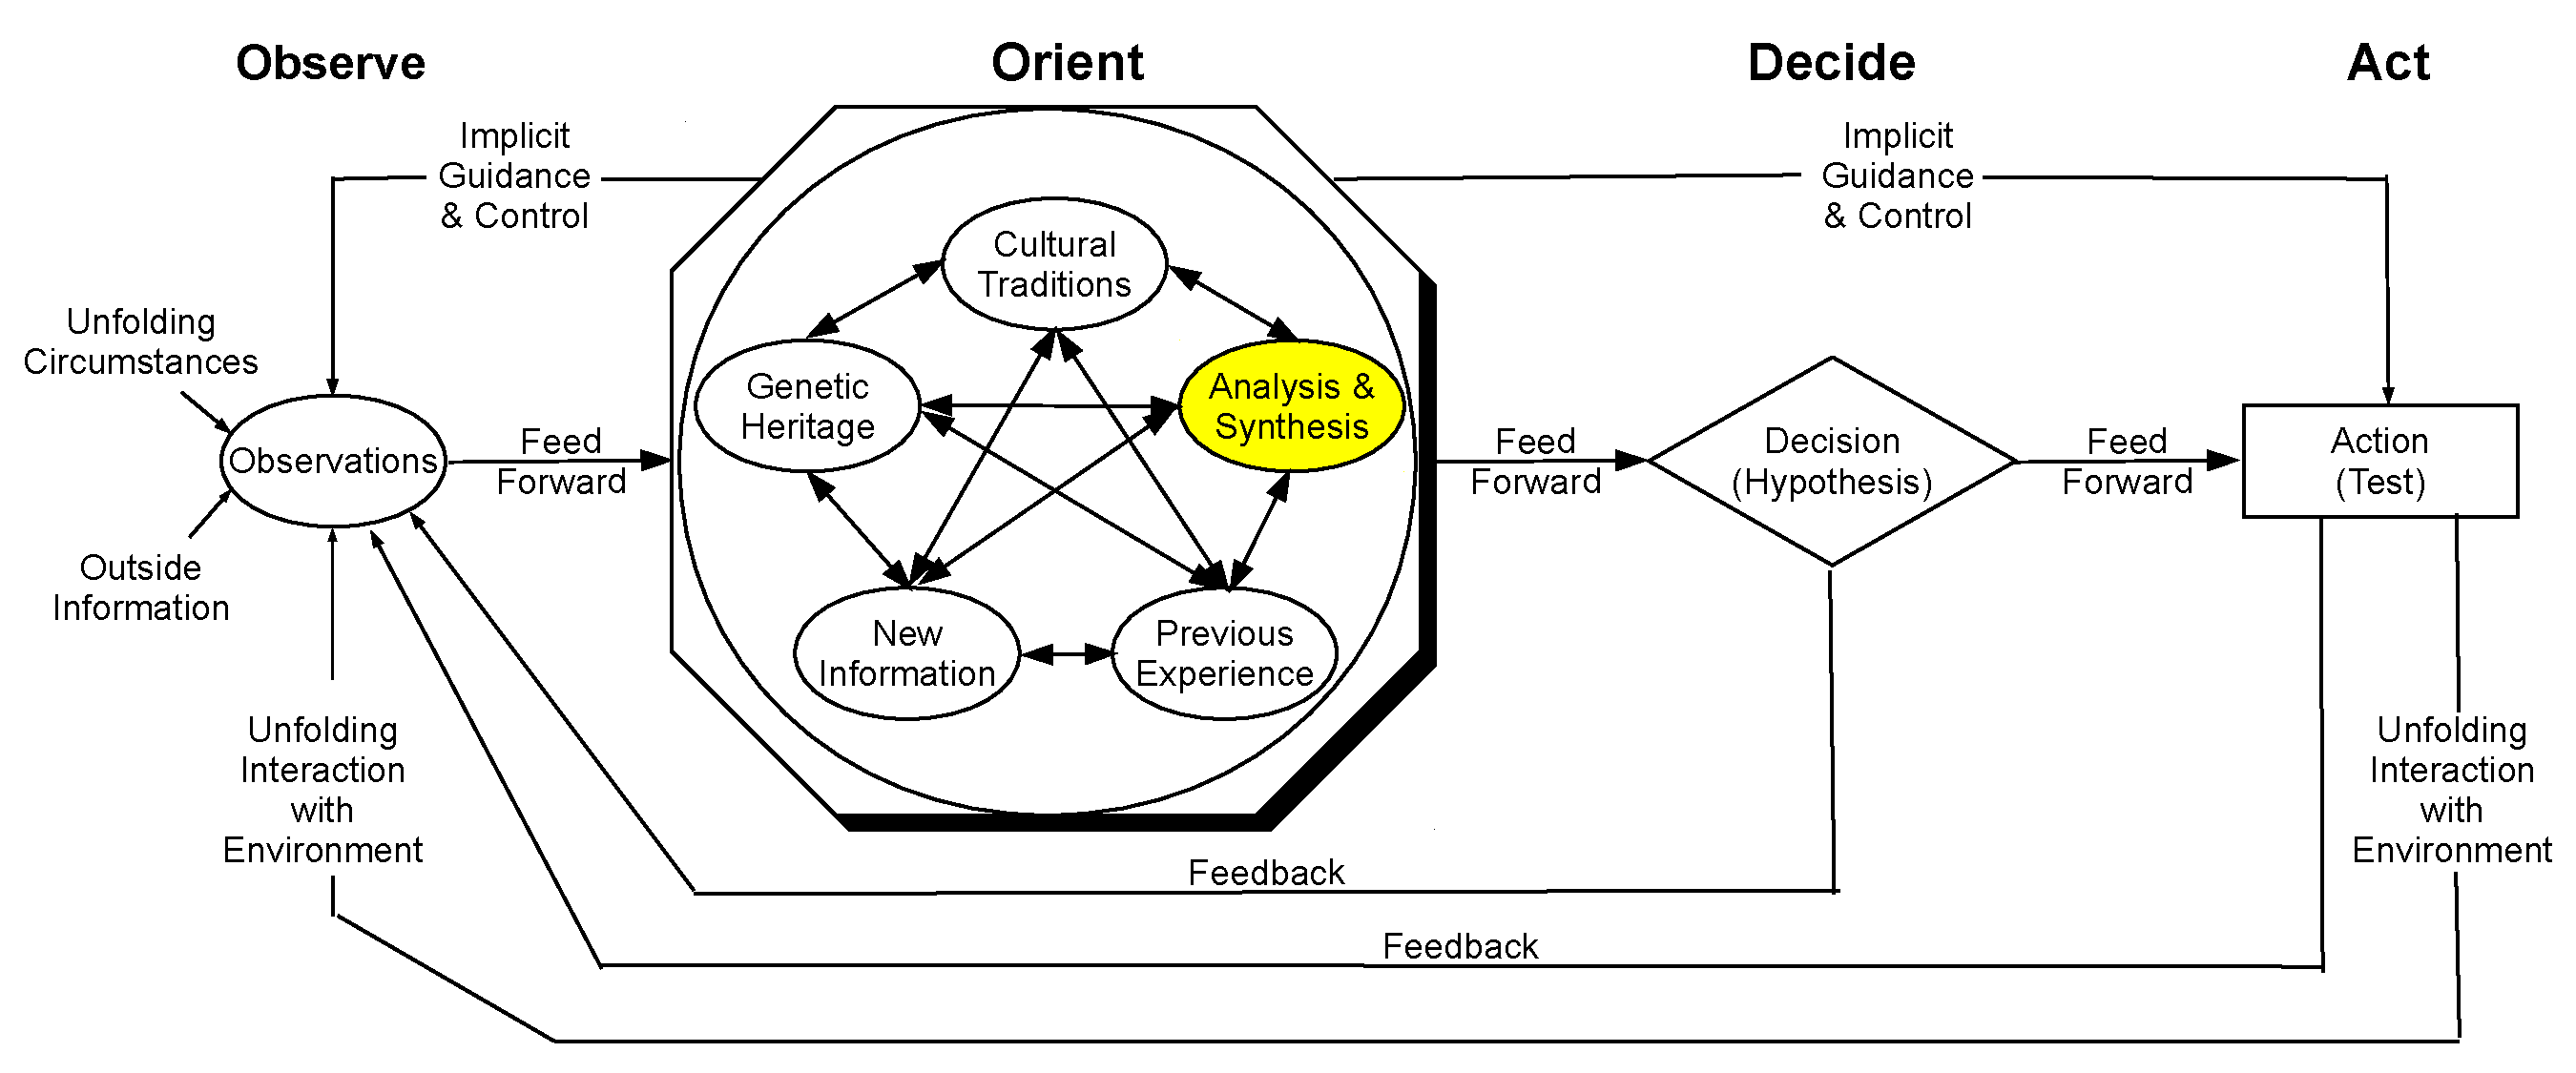
\includegraphics[width=0.9\linewidth]{Figures/Introduction/OODA}
  \caption{John Boyd's OODA Loop}
  \label{fig:ooda-loop}
\end{figure}

\begin{figure}[tb]
  \centering
  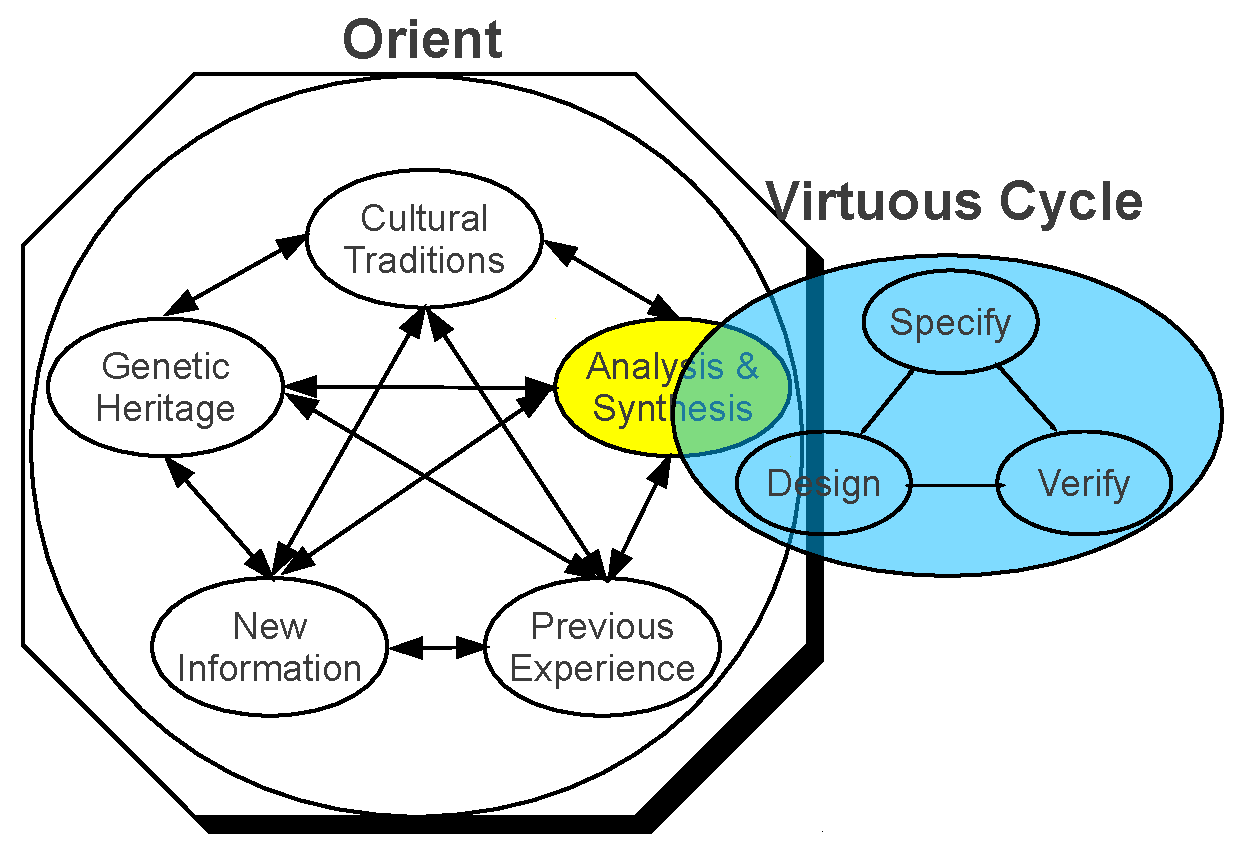
\includegraphics[width=0.6\linewidth]{Figures/Introduction/OrientVirtuousCycle}
  \caption{Orientation and the Virtuous Cycle}
  \label{fig:orient-virtuous-cycle}
\end{figure}
% ---- this points LaTeX to book.tex ---- 
% Local Variables: 
% TeX-master: "book"
% End:



\part{Preliminaries}


\chapter{Reasoning about Access Control}
\label{chap:access-control}

% ---- this points LaTeX to book.tex ---- 
% Local Variables: 
% TeX-master: "book"
% End:

\chapter{Digital Authentication}
\label{cha:pki}

% \suebox{Digital authentication using PKI is well suited for
%   authentication in distributed environments such as the internet.  We
%   present some of the details here, and how they are expressible in the
%   logic.} \vspace*{1em}

% \section{Digitally Signed Statements and Authority}
% \label{sec:digital-signatures}

%\subsection{Authentication}
%\chapter{Digital Authentication}

To make reasoned access-control decisions in a digital world, we need
to explore in more depth how statements are signed and authenticated
digitally.  The basis for digital signatures rests on cryptographic
keys and cryptographic hash functions in general, and on public-key
cryptography in particular. Digital authentication using
\mainindex{PKI|see{public-key infrastructure}}public-key infrastructure
(PKI) is well suited for authentication in distributed environments
such as the Internet.

In this chapter, we describe the details of digital authentication using
the access-control calculus.  Unlike traditional explanations, we do not
go into the algorithmic details of any particular encryption or hash
function. Rather, we describe the relationship between public and
private keys, encryption and decryption, keys and principals, and
certificates.

% In addition to the discussion on digital signatures, we also develop the
% concept of recognizing authority, which we call \emph{jurisdiction}.  As
% we will see later on in this section, acquiring a belief in a statement
% or cryptographic key usually requires two components: first, a statement
% attributable to some authority, and second, jurisdiction and trust in
% the integrity of the authority making the statement.

\section{Public-Key Cryptography}
\label{sec:pubkey-crypto}


\mainindex{cryptography!public-key cryptography}At the core of
public-key cryptography are two cryptographic keys: one is
\mainindex{public-key infrastructure!public key}\emph{public} and is
openly shared (much like a telephone number or email address), and the
other is \mainindex{public-key infrastructure!private
  key}\emph{private} and must be known \emph{only} by a single
principal. In theory, the principal who possesses the private key is
the only principal who can decrypt messages that were encrypted using
the corresponding public key.  This property is used to ensure
\mainindex{privacy}\emph{privacy}: that is, only a principal with the
correct private key can read a message. Similarly, messages encrypted
using a private key can be universally decrypted by anyone who
possesses the corresponding (and publicly disclosed) public key.  This
property is used for \mainindex{authenticity}\emph{authenticity}: that
is, one can establish the identity of the author of a message.

The public key $K$ and private key $K^{-1}$ together form a
\mainindex{public-key infrastructure!key pair}\emph{key pair}
$(K,K^{-1})$, and each key can undo the actions of the other.  That
is, if \emph{encrypt} and \emph{decrypt} are particular encryption and
decryption functions, then the following properties must hold for all
messages $m$:
\begin{eqnarray*}
  \mathit{decrypt}(K^{-1},\mathit{encrypt}(K,m)) & = & m, \\
  \mathit{decrypt}(K, \mathit{encrypt}(K^{-1},m)) & = & m. 
\end{eqnarray*}
In addition, the public and private keys are typically distinct (i.e.,
$K^{-1} \neq K$).  Consequently, public-key cryptography is often
referred to synonymously as \mainindex{asymmetric-key
  cryptography}\emph{asymmetric-key cryptography}.  In the case of
public-key algorithms such as RSA \cite{RSA}, the same algorithm
serves both to encrypt and decrypt messages.

\mainindex{cryptography!cryptosystem, key properties of}There are two additional
properties about encryption and decryption that are important if a
cryptosystem is to be useful:
\begin{enumerate}
\item It should be computationally infeasible to read an
  encrypted message without knowing the correct decryption key.  

  That is, given an encrypted message $\mathit{encrypt}(K_e,m)$, it
  should be computationally infeasible to determine $m$ without knowing
  the reciprocal key $K_d$.  (Note that $K_e$ may be either a public or
  private key; $K_d$ is the other half of the key pair.)
\item It should be computationally infeasible to successfully forge an
  encryption without knowing the encryption key $K_e$.

  That is, given a message $m$ but without knowing $K_e$, it should be
  computationally infeasible 
  to compute an $\mathit{x}$ such that $\mathit{decrypt}(K_d,x) = m$.  
\end{enumerate}

\mainindex{privacy!use of cryptography for}These properties of
public-key cryptography support privacy in the following way.  If
Alice wishes to send a message to Bob that only Bob can read, she
encrypts the message with Bob's \emph{public key} $K_{\name{Bob}}$.
Thus, Alice sends to Bob the following:
\[ \mathit{encrypt}(K_{\name{Bob}},\mathrm{message}). \]
The idea here is that the resulting cipher text should
be decipherable only with knowledge of Bob's \emph{private key}
$K_{\name{Bob}}^{-1}$.  Upon receipt, Bob uses his private key to
decrypt the message:
\[
\mathit{decrypt}(K^{-1}_{Bob},\mathit{encrypt}(K_{\name{Bob}},\mathrm{message})). \] 
Figure~\ref{fig:public key} illustrates schematically how Alice and Bob
use Bob's keys to ensure privacy of the message sent to Bob.

% More
% precisely, if $K_{\name{Bob}}$ is Bob's public key available to all, and
% $K^{-1}_{Bob}$ is Bob's private key known only to Bob:
% \begin{eqnarray*}
%   \textsf{Private message sent to Bob} & = & \mathit{encrypt}(K_{\name{Bob}},\mathrm{message})\\
%   \textsf{Deciphered message} & = & \mathit{decrypt}(K^{-1}_{Bob},\mathit{encrypt}(K_{\name{Bob}},\mathrm{message}))
% \end{eqnarray*}

\begin{figure}[tbp]
  \centering
  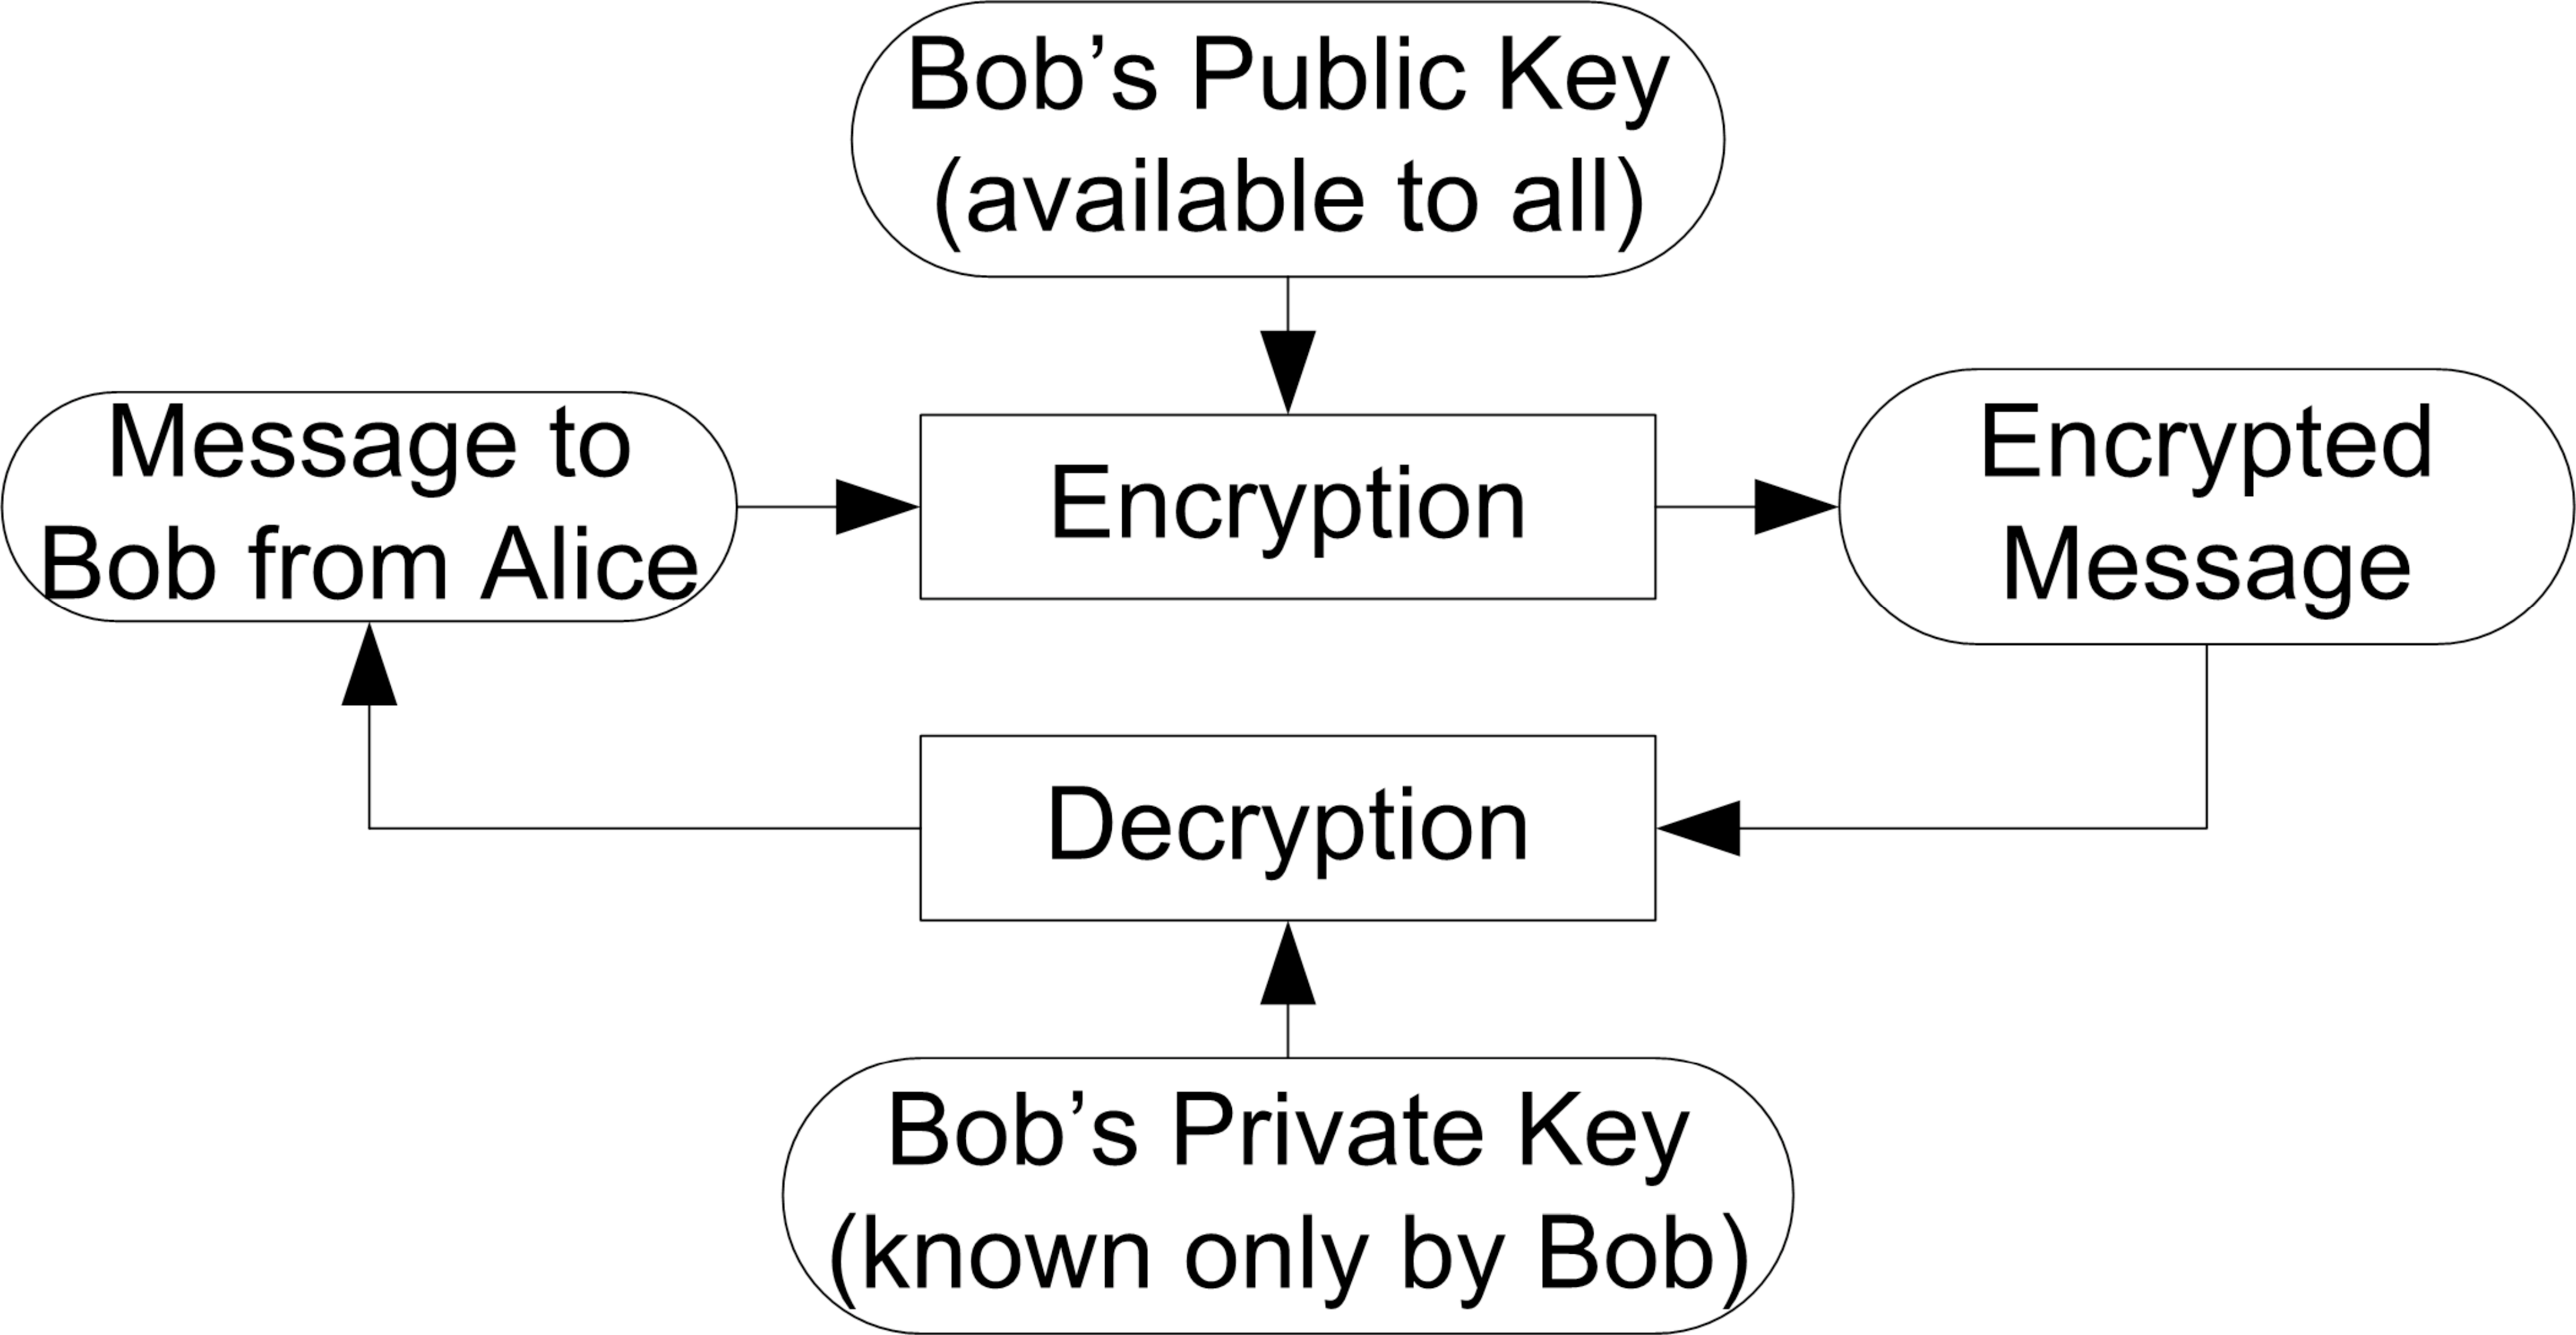
\includegraphics[width=3.5in]{Figures/pki/publicKey}
  \caption{Process for using public-key encryption for privacy}
  \label{fig:public key}
\end{figure}


The use of public-key cryptography is not limited solely to achieving
privacy. More often, it is used to authenticate messages, such as
website-connection requests, public-key certificates, and so on.  For
example, suppose that Bob wishes to communicate a message to the world
in such a way that anyone can deduce that Bob authored the message. Such
a situation might arise if Bob needs to establish his authorship of an
article or book for intellectual-property protection.  In this case, Bob
can encrypt his book using his \emph{private key} (which is known only
by him):
\[ \mathit{encrypt}(K^{-1}_{\name{Bob}}, book). \]
Anyone who cares to read
Bob's book can read it using Bob's freely available \emph{public
  key} to decrypt his encrypted file:
\[ \mathit{decrypt}(K_{\name{Bob}},\mathit{encrypt}(K^{-1}_{Bob},
book)). \] The idea here is that \emph{only} Bob could have created the
original encrypted file, because only Bob knows the key
$K^{-1}_{\name{Bob}}$ used to create it.  This sort of use of public-key
  cryptography for authenticity is illustrated in
  Figure~\ref{fig:private key}.
% \begin{eqnarray*}
%   \textsf{Book authored by Bob} & = & \mathit{encrypt}(K^{-1}_{Bob}, book)\\
%   \textsf{Book accessible by Bob's public key} & = & \mathit{decrypt}(K_{\name{Bob}},\mathit{encrypt}(K^{-1}_{Bob}, book))
% \end{eqnarray*}

\begin{figure}[tbp]
  \centering
  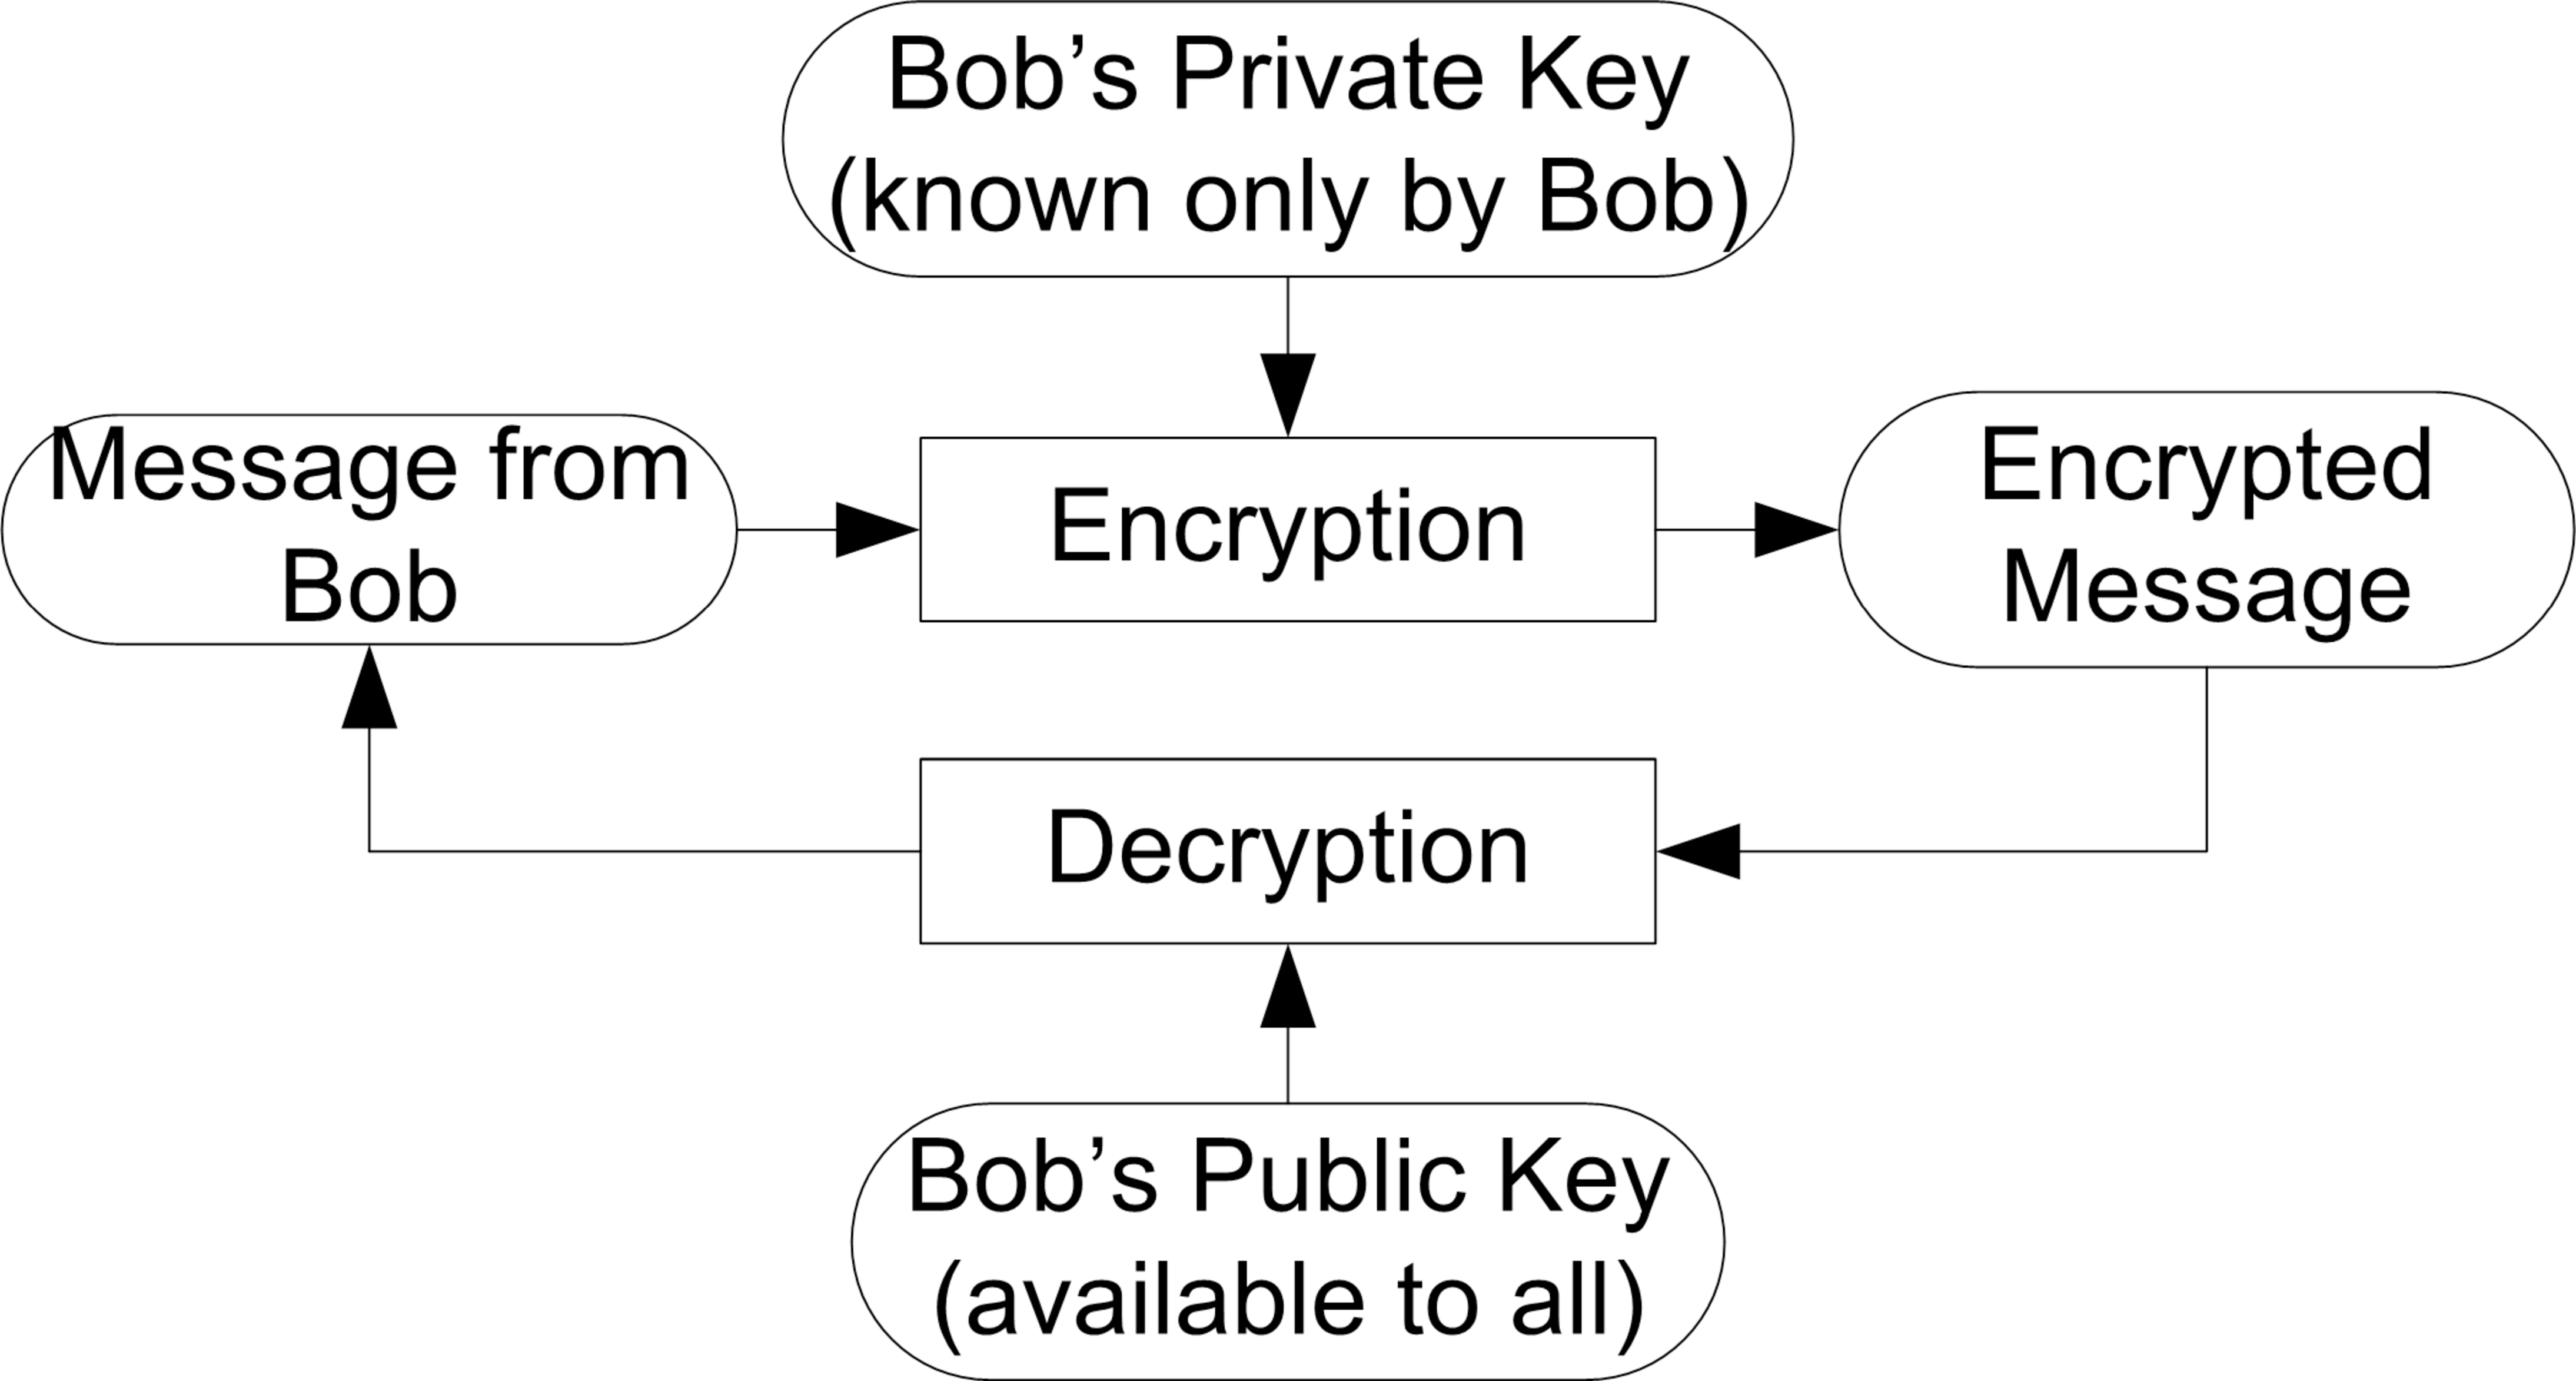
\includegraphics[width=3.5in]{Figures/pki/privateKey}
  \caption{Process for using private-key encryption for authenticity}
  \label{fig:private key}
\end{figure}

\mainindex{authenticity!use of cryptography for}One can combine these
two approaches to achieve a combination of \mainindex{privacy}privacy
and \mainindex{authenticity}authenticity.  For example, suppose that
Alice wants to send a message that only Bob can read, while providing
Bob assurance that the message is coming from her.  To achieve this
goal, Alice employs the following three-step process:
\begin{enumerate}
\item Alice encrypts her message $m$ with her \emph{private key}:
  \[ \mathit{encrypt}(K^{-1}_{\name{Alice}},m). \] This step will allow
  Bob to deduce that Alice authored the message $m$, because Bob can
  retrieve $m$ using Alice's \emph{public key}.
\item Alice encrypts the result from step one with Bob's \emph{public
    key}, resulting in the following:
  \[
  \mathit{encrypt}(K_{\name{Bob}},\mathit{encrypt}(K^{-1}_{\name{Alice}},m)).
  \]
  This step provides Alice with assurance that only Bob can read her
  message, because only Bob's private key will be able to decrypt this
  cipher text.
\item Alice informs Bob in plain text that she is the author of the
  cipher text from step two.  This hint tells Bob to look up Alice's
  public key so that he can decipher the message in such a way as to be
  assured that Alice was the author.  
\end{enumerate}

\section{Efficiency Mechanisms}
\label{sec:digital-signatures}
In theory, the approaches described in the previous section are
sufficient to handle the needs of privacy and authenticity. In practice,
however, the approaches described for authenticity are rarely used,
because public-key algorithms are relatively slow and costly to use.  In
addition, the repeated use of a given key-pair on large amounts of text
can expose the keys and make them vulnerable to cryptographic analysis
and discovery. To address these pragmatic concerns, two additional steps
can be taken: (1) we can use a \emph{cryptographic hashing} algorithm,
and (2) we can use a \emph{session} or \emph{data-encryption key}
(DEK). We describe these steps---and their use in creating and verifying
digital signatures---in this section.

\subsection{Cryptographic Hash Functions}

% \begin{figure}[tbp]
%   \centering
%   \includegraphics{Figures/basicACConcepts/hash}
%   \caption{Hash functions}
%   \label{fig:hash functions}
% \end{figure}

% Cryptographic hash functions take arbitrarily large files and return a
% fixed-length number (e.g., 128-bits). % This is shown in
% % Figure~\ref{fig:hash functions}. 

% Hash functions are widely used, but not all are cryptographic in nature.
% An odd parity bit that is set when there is an odd number of $1$'s
% stored in a memory location is a hash function that is not cryptographic
% in nature.  For example, consider an odd parity bit for 4-bit words.
% The 4-bit words that would set the parity bit to a $1$ are as follows:
% $0001$, $0010$, $0100$, $1000$, $0111$, $1011$, $1101$, $1101$, and
% $1110$.  The predictability of the odd parity bit function disqualifies
% it as a cryptographic hash.  If the parity bit is $1$, then the input is
% one of the nine 4-bit numbers above.  If the parity bit is $0$, then it
% is one of the remaining seven 4-bit numbers that have an even number of
% $1$'s or all $0$'s.

Hash functions are commonly used in computing as a way to map large data
spaces to more compact spaces, substituting uniqueness for efficiency.
A very simple example of a hash function is a word-level \emph{parity
  check}: all $32$-bit words with an even number of $1$ bits are mapped
to the bit $0$, while all those with an odd number of $1$ bits are
mapped to the bit $1$.  In this case, a data space with $2^{32}$
elements is mapped to a data space of $2$ elements, at the cost of
uniqueness: $2^{16}$ values are hashed to the bit $0$, and $2^{16}$
values are hashed to the bit $1$.

\mainindex{hash function, cryptographic}\emph{Cryptographic hash
  functions} are hash functions with an additional property: given any
particular hash value, it must be \emph{computationally infeasible} to
determine an input that, when hashed, produces the given value.  This
property is known as the \mainindex{hash function,
  cryptographic!one-way property}\emph{one-way property} of
cryptographic hashes: while hash values can be computed easily from a
given input, it is computationally infeasible to do the reverse (i.e.,
compute an input that produces a particular hash value).  Thus, for
example, the parity check clearly fails the one-way property (and
hence would not make for a cryptographic hash function), because it is
trivial to find 32-bit words with parity $1$.

The one-way property of cryptographic hashes makes it possible for
fixed-length cryptographic hash values to simulate unique identifiers
for messages of arbitrary length.  For example, suppose Ellen wants to
send a file to Todd that is several megabytes in length, and she wants
Todd to be able to determine whether the file he receives has arrived
unchanged and uncorrupted.  To accomplish this goal, Ellen sends a
\mainindex{hash function, cryptographic}\emph{cryptographic hash} of
the file---also known as the \mainindex{hash function,
  cryptographic!checksum}\emph{cryptographic checksum}---along with
the file itself:
\[ (\mathit{file}, \textit{cryptographic checksum}).\] When Todd receives
the file and the cryptographic checksum, he applies the hash algorithm
to the received file and compares the value he computed with the
checksum sent by Ellen.  If they both match, then Todd concludes that the
file he received is intact and free of any tampering or corruption.


\subsection{Data-Encryption Keys}
When privacy is also a concern for a large file, the sender may elect
to also employ a \mainindex{symmetric key}\emph{symmetric-key}
encryption algorithm---such as the Advanced Encryption Standard (AES)
\cite{AES}---to create a one-time \mainindex{data-encryption
  key}data-encryption key $K_{dek}$.  Symmetric-key encryption
algorithms use the same key for both encryption and decryption (i.e.,
$K_{dek} = K^{-1}_{dek}$).  In addition, symmetric-key encryption
algorithms are three orders of magnitude faster than typical
public-key algorithms, because of the underlying operations they
employ (i.e., exclusive-or and bit substitutions as opposed to
modulo-$n$ exponentiation).

% If privacy is a concern as well as not overusing public keys on large
% files, what Ellen can do is create a one-time data-encryption key
% $K_{dek}$ for a \emph{symmetric} key encryption algorithm such as the
% Advanced Encryption Standard (AES) \cite{AES}.  Symmetric key encryption
% algorithms are called symmetric because the same key is used for both
% encryption and decryption. In other words, $K_{dek} = K^{-1}_{dek}$.

If Ellen chooses this approach, she first creates a key $K_{dek}$; she
then encrypts the file with $K_{dek}$, computes the cryptographic
checksum of the file, and encrypts $K_{dek}$ with Todd's public key
$K_{\name{Todd}}$. Ellen sends these three items to Todd:
\[ \mathit{encrypt}(K_{\name{Todd}},K_{dek}), \qquad
\mathit{hash}(\mathit{file}), \qquad \mathit{encrypt}(K_{dek},
\mathit{file}). 
\]
% \begin{eqnarray*}
%   \textsf{Data Encryption Key encrypted for Todd} & = & \mathit{encrypt}(K_{\name{Todd}},
%   K_{dek}) \\
%   \textsf{File encrypted with }K_{dek} & = & \mathit{encrypt}(K_{dek}, file)\\
%   \textsf{Cryptographic Checksum} & = & hash(file)
% \end{eqnarray*}
When Todd receives these three items, he first retrieves the
data-encryption key $K_{dek}$ by using his private key:
\[ \mathit{decrypt}(K^{-1}_{\name{Todd}},\mathit{encrypt}(K_{\name{Todd}},
K_{dek})) = K_{dek}. \]
He then uses the data-encryption key to retrieve the file:
\[ \mathit{decrypt}(K_{dek},\mathit{encrypt}(K_{dek},\mathit{file})) = \mathit{file}.\]
Finally, he checks the integrity of the retrieved file by determining
whether it hashes to the cryptographic checksum that Ellen sent.  

Unfortunately, however, this scheme is subject to fraud, because none of
the sent items directly tie Ellen to the message that Todd receives.  As
a result, a third party could send their own message (along with its
cryptographic checksum) to Todd, alleging that the message is from
Ellen. Todd has no way of determining the truth of such a claim.  We
can address this problem by introducing digital signatures in the
next subsection.

\subsection{Digital Signatures}

\begin{figure}[tbp]
  \centering
  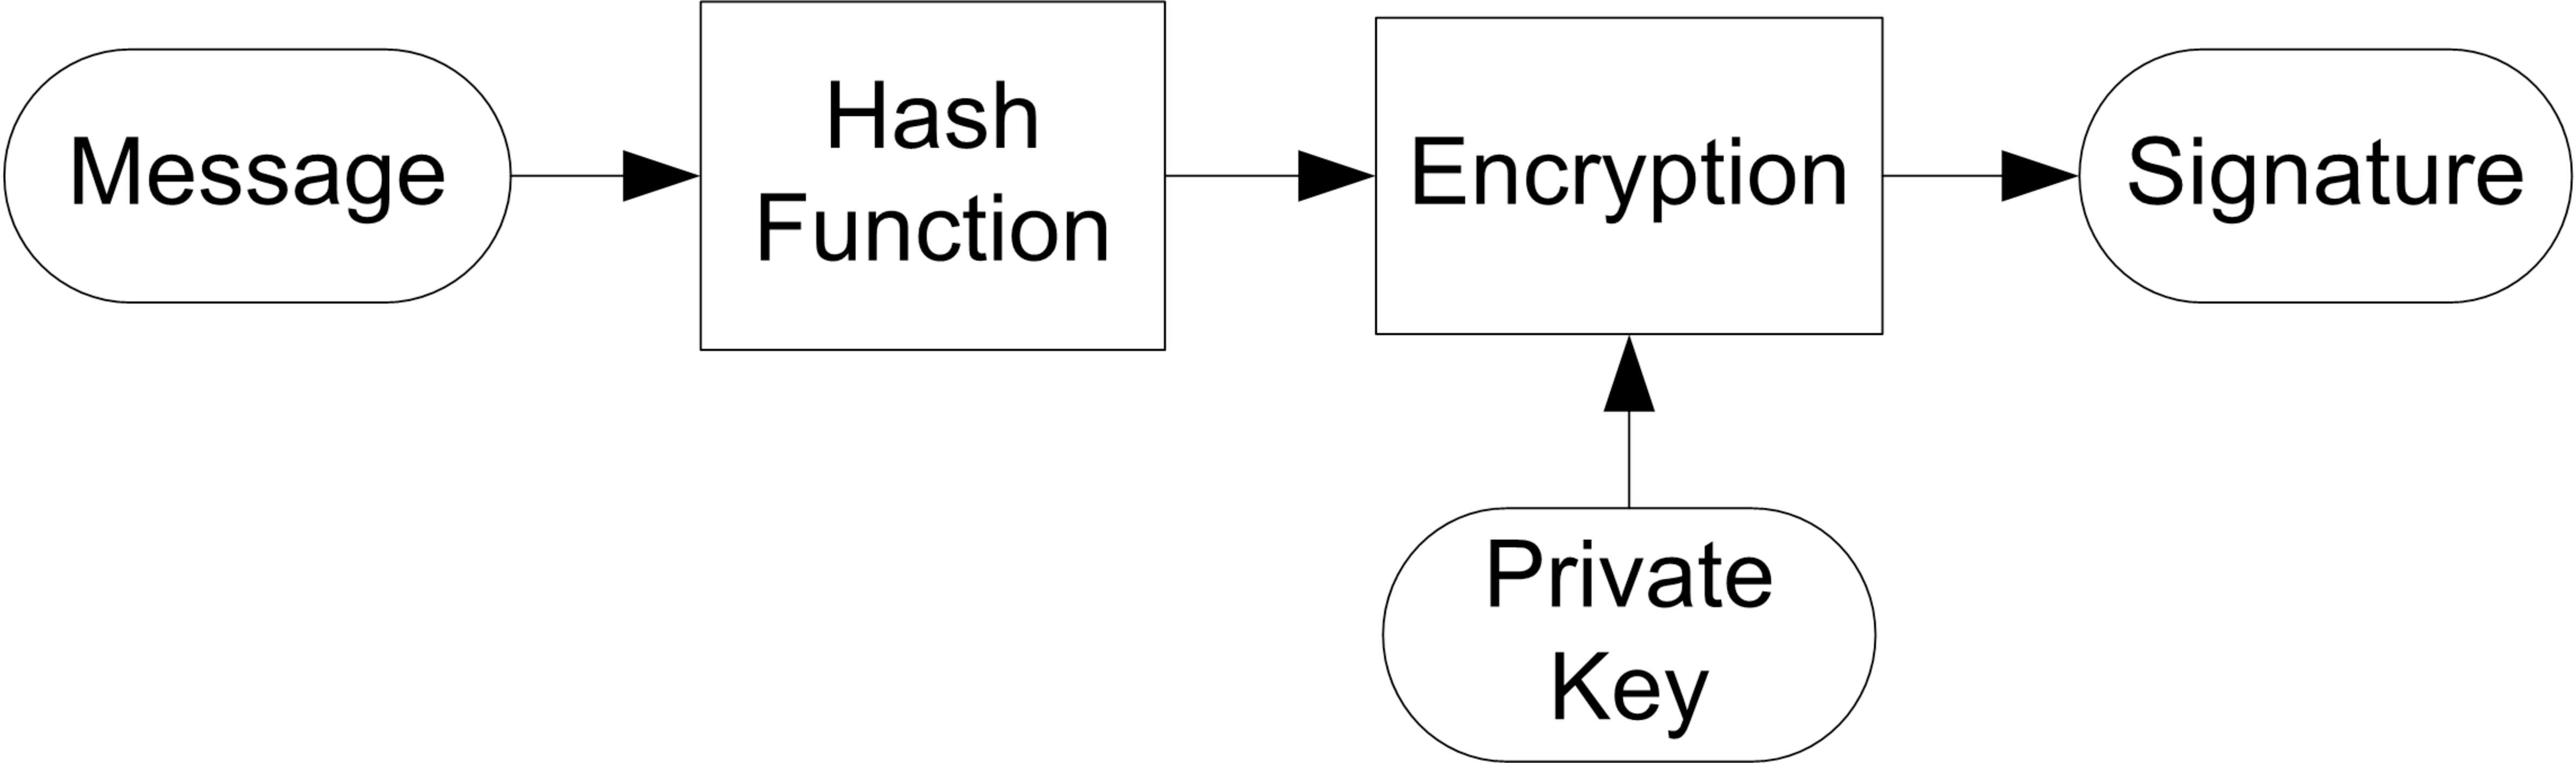
\includegraphics[width=3.5in]{Figures/pki/signature}
  \caption{Process for creating a digital signature}
  \mainindex{digital signature}
  \label{fig:digital signature}
\end{figure}

We can fix the potential fraud problem by one addition: Ellen creates
a \mainindex{digital signature}\emph{digital signature} by encrypting
the cryptographic checksum with her \emph{private key}.
Figure~\ref{fig:digital signature} illustrates a process for creating
digital signatures that supports both integrity and authorship:
\begin{enumerate}
\item The message or file is hashed by a one-way function. The resulting
  fixed-length hash value identifies the contents of the message.
\item The hash value is then encrypted using the \emph{private} key of
  the sender. The encrypted hash value identifies the sender, because
  the hash value can be retrieved only by using the sender's public
  key.  Note that, because the hash value is much smaller than the
  message itself, this approach is much more efficient than the process
  described in Section~\ref{sec:pubkey-crypto}.
\end{enumerate}
Unlike human signatures, which remain relatively unchanged over time,
digital signatures change depending on the contents of what is being
signed.

\begin{figure}[tbp]
  \centering
  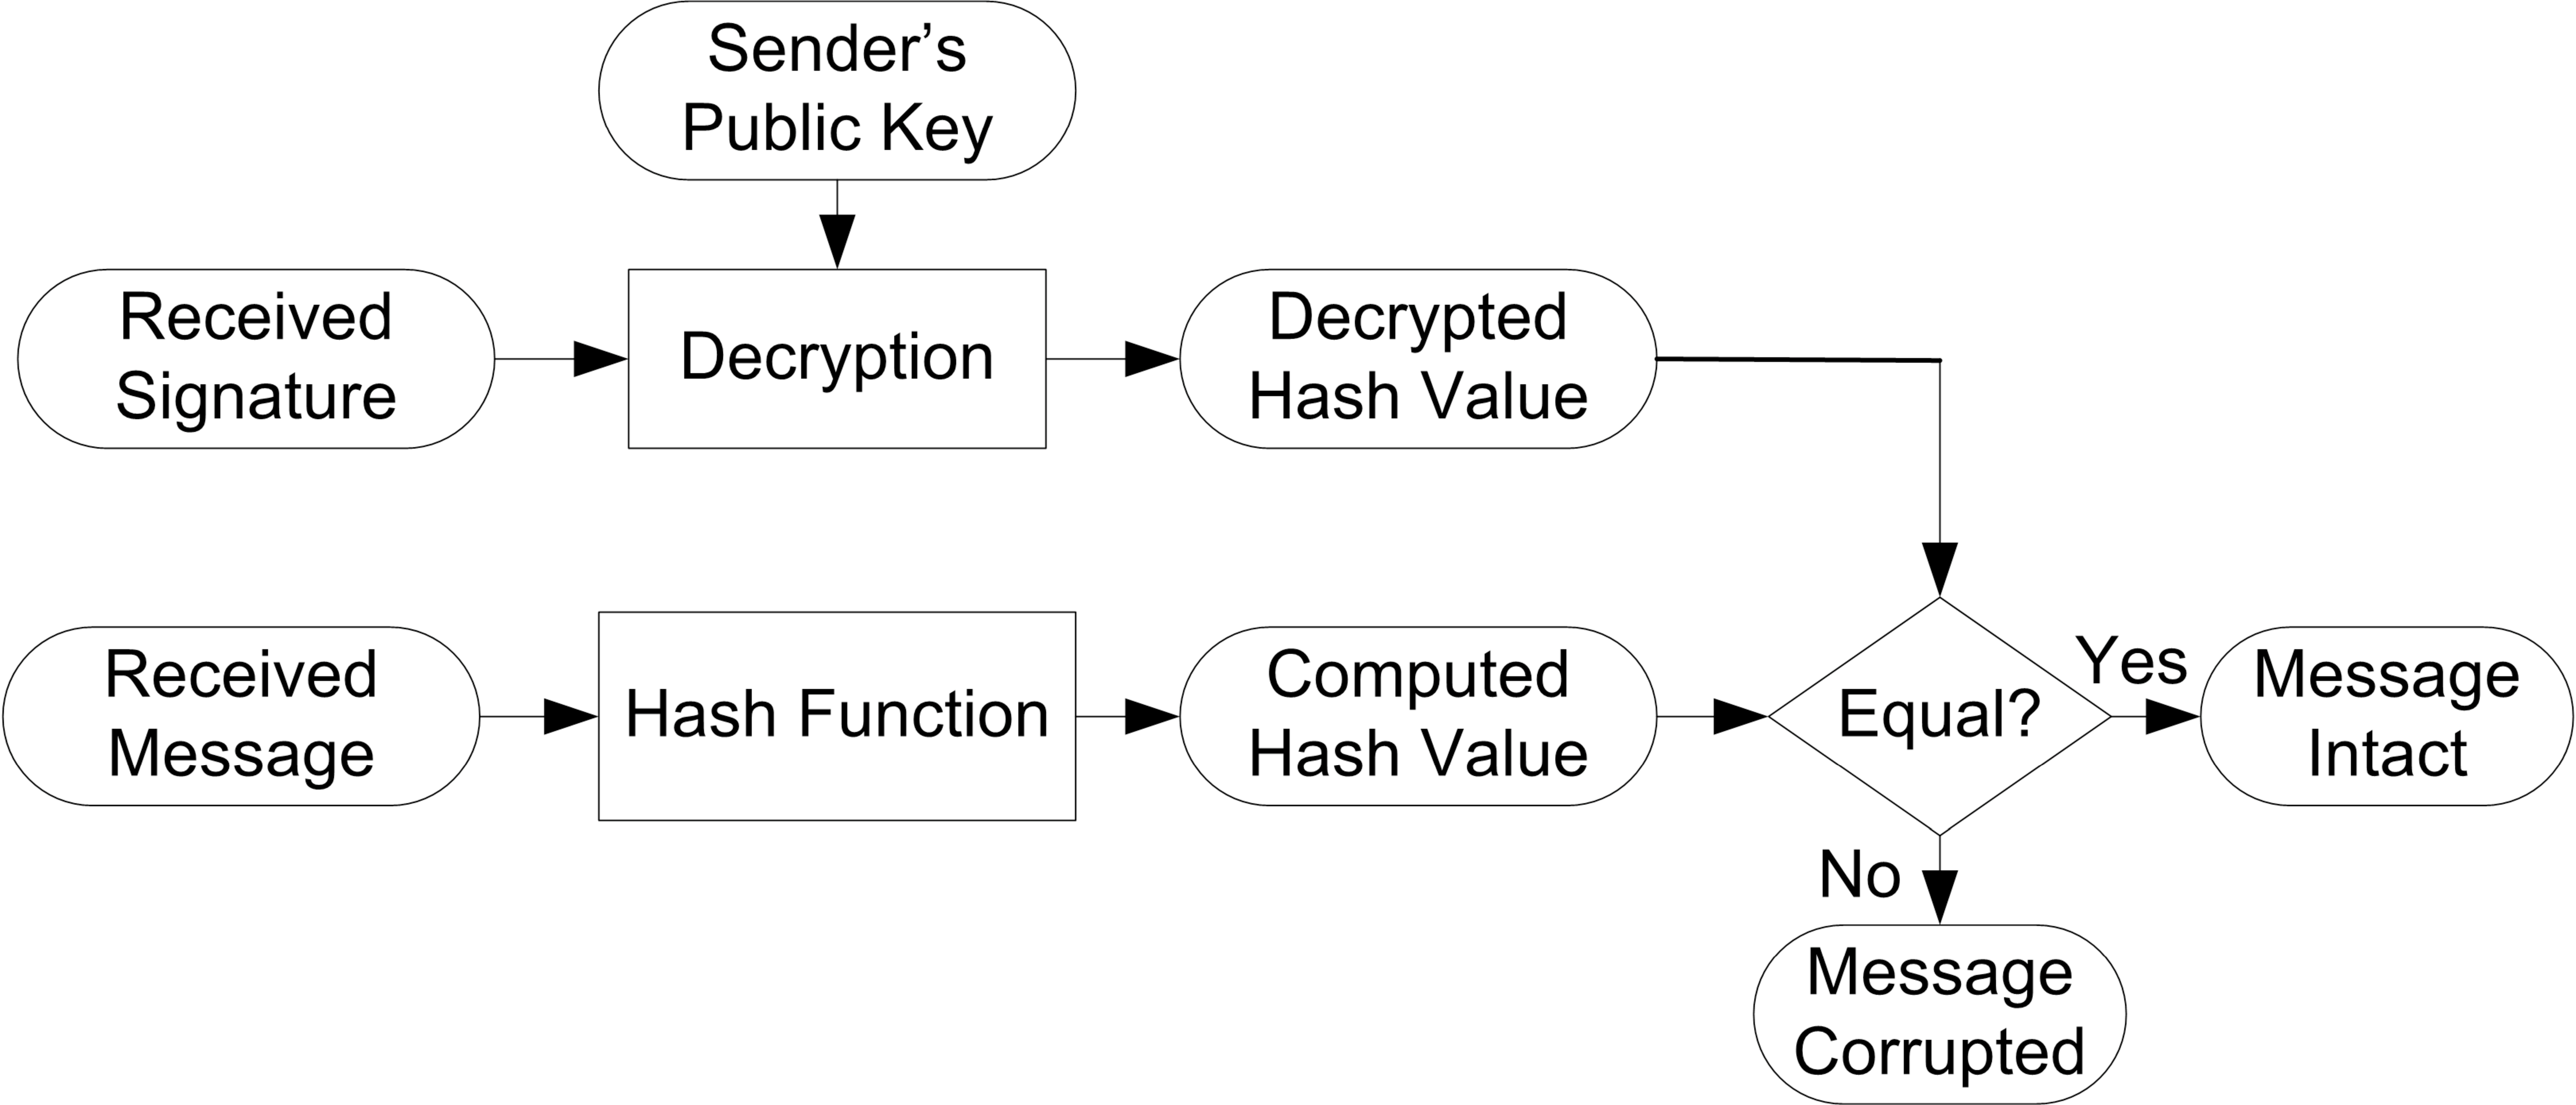
\includegraphics[width=4.5in]{Figures/pki/signatureCheck}
  \caption{Process for verifying a digital signature}
  \mainindex{digital signature}
  \label{fig:signature verification}
\end{figure}

\mainindex{digital signature}Figure~\ref{fig:signature verification}
illustrates the process of verifying a digital signature.  The process
simply compares the following two values: (1) the hash value obtained
by decrypting the received signature using the sender's public key,
and (2) the hash value obtained by hashing the contents of the
received message.  If the values match, then the received message is
considered to be both intact and from the public key's owner.



\section{Reasoning about Cryptographic Communications}
In the previous two sections, we have seen how cryptography can be used
to provide assurances of privacy and authenticity in distributed digital
systems.  In this section, we see how the access-control logic can be
used to express and reason about cryptographic communications.

As an example, suppose that Ellen uses the methods described in
Section~\ref{sec:digital-signatures} to send Todd a digitally signed
message.  For this first case, let us imagine that Ellen sends the
message itself in the clear (i.e., in plaintext with no encryption), but
she digitally signs it.  Thus, she sends to Todd the following
combination of items:
\[ m,\quad \mathit{encrypt}(K^{-1}_{\name{Ellen}},hash(m)).\]
That is, she sends the message $m$, along with the encrypted hash (i.e.,
cryptographic checksum) of $m$. 

When Todd receives the message, he applies the \mainindex{authentication!message
  integrity, formalization in logic} signature-verification protocol
of Figure~\ref{fig:signature verification}.  If this process is
successful, then Todd has evidence that Ellen's public key
$K_{\name{Ellen}}$ has been used to verify that the message $m$
arrived intact and uncorrupted.  This fact can be expressed in the
access-control logic by recognizing $m$ as a statement made by
$K_{\name{Ellen}}$:
\[ K_{\name{Ellen}} \says m .\]
If Todd believes that  $K_{\name{Ellen}}$ is Ellen's public key---perhaps
he looked her key up in a public directory, or perhaps Ellen gave it to
him sometime in the past---then he is willing to associate statements
made (i.e., integrity-checked) by that key with Ellen.  Thus, the belief
that Ellen's public key is $K_{\name{Ellen}}$ can be expressed in the
logic as the following statement:
\[ K_{\name{Ellen}} \speaksfor \name{Ellen} . \] Based on these two
factors, Todd can deduce that Ellen originally sent the message $m$.  In
terms of the logic, this analysis uses the \infname{Derived Speaks For}
rule, as shown in the proof of
Figure~\ref{fig:dig-sig-proof}.

\begin{figure}
  \centering
  \begin{formalProof}
    1. $K_{\name{Ellen}} \says m$ & Received message with signature verified
    using $K_{\name{Ellen}}$\\
    2. $K_{\name{Ellen}} \speaksfor Ellen$ & Ellen's public key\\
    3. $Ellen \says m$ & 2, 1 Derived speaks for
  \end{formalProof}
  \caption{Simple analysis of digital signatures}
  \label{fig:dig-sig-proof}
\end{figure}

Having examined the simpler case, now let us consider the case where
Ellen sends Todd a digitally signed message, using a data-encryption key
$K_{dek}$ to encrypt the message.  Recall that Todd receives three items,
along with a hint that Ellen is the sender:
\[ \mathit{encrypt}(K_{\name{Todd}}, K_{dek}), \quad
\mathit{encrypt}(K_{dek},m), \quad
\mathit{encrypt}(K^{-1}_{\name{Ellen}},hash(m)). \]
Todd must decrypt the first component of this package to
obtain the key $K_{dek}$, which he can then use to retrieve the message
$m$.  He then verifies Ellen's digital signature by computing the
cryptographic hash of $m$ and comparing it with the checksum that Ellen
sent.  

If this process is successful, then Todd once again used Ellen's public
key to verify that the message $m$ he received was indeed the one
initially signed by Ellen.  As we saw earlier, this situation can be
expressed simply as follows:
\[ K_{\name{Ellen}} \says m .\]
Although the signature-verification process itself may be more involved
in this situation, it plays the same role in Todd's interpretation of the
received message.  From Todd's perspective, the important aspect is
deducing that the message was initially signed by Ellen using the key
$K^{-1}_{\name{Ellen}}$, which presumably only she possesses. Although
he initially had to decrypt other components of the message using the
keys $K^{-1}_{\name{Todd}}$ and $K_{dek}$, those operations alone do
not associate the message $m$ to Ellen.


% \begin{example}
%   How do we represent this in the access-control calculus? The answer is
%   we represent it as $Ellen \says m$, exactly as it we did in the
%   previous example!  The reason is that from Todd's perspective, what is
%   important is deducing that $m$ as received by Todd was in fact signed
%   by Ellen using $K^{-1}_{\name{Ellen}}$, which presumably only Ellen
%   possesses. While Todd did decrypt both $K_{dek}$ and $m$ using
%   $K^{-1}_{\name{Todd}}$ and $K_{dek}$ respectively, these operations themselves
%   do not contribute anything to an argument attributing $m$ to Ellen.
%   Of significance was verifying the signature using $K_{\name{Ellen}}$ and
%   knowing that $K_{\name{Ellen}} \speaksfor Ellen$.
% \end{example}

%\subparagraph{Integrity-Checked Messages}

These two examples provide a general framework for expressing digitally
signed and verified statements in our logic.    
Whenever a digitally signed message $m$ has been verified
using the key $K_P$ in a process such as the one shown in
Figure~\ref{fig:signature verification}, we represent the message as
\[K_P \says m. \]
We can express the belief that the key $K_P$ is associated with the
principal $P$ as follows:
\[ K_P \speaksfor P. \]
Finally, the \infname{Derived Speaks For} rule allows us to conclude that $m$
originated from the principal $P$:
\[P \says m. \] The important aspect about this abstraction is that it
moves beyond the details about signature verification and focuses our
attention on who said what.

\section{Certificates,  Certificate Authorities, and Trust}

In the examples of the previous section, Todd's reasoning depended
crucially upon his assumption that $K_{\name{Ellen}}$ was Ellen's key:
\[K_{\name{Ellen}} \speaksfor Ellen. \]
% In other words, $K_{\name{Ellen}}$ was Ellen's proxy speaking for her when it
% came to digitally signing messages.
What we have not directly addressed is how Todd---or anyone else, for that
matter---would come to believe 
that $K_{\name{Ellen}}$ is Ellen's public key.  

In most cases, such a belief originates from a \mainindex{certificate!public-key
  certificate}\emph{public-key certificate}, which is issued by an
alleged authority called a \mainindex{certificate!certificate
  authority}\emph{certificate authority} (or \emph{CA}, for short).  A
public-key certificate is a digitally signed statement that associates
a given public key with a given principal.  \mainindex{certificate!public-key
  certificate!formalization in logic}A certificate that associates the
public key $K_P$ with principal $P$ can be expressed in the logic as
\[ K_{CA} \says (K_P \speaksfor P), \] where $K_{CA}$ is the public key
of the issuing certificate authority.  \mainindex{public-key
  infrastructure!public-key certificate|see{certificate}}

Although digital certificates such as these provide necessary
information, they alone are insufficient to establish why Todd would
believe that $K_{\name{Ellen}} \speaksfor Ellen$.  Rather, such beliefs
also depend on recognition of the certificate authority and their
jurisdiction.  For example, 
suppose that Cora issues a
certificate signed with her private key $K^{-1}_{Cora}$:
\[K_{\name{Cora}} \says (K_{\name{Ellen}} \speaksfor Ellen). \]
Furthermore, suppose that Todd believes that $K_{\name{Cora}}$ is
Cora's public key:
\[K_{\name{Cora}} \speaksfor \name{Cora}. \]
From these two pieces of information, Todd is able to conclude the
following:
\[ \name{Cora} \says (K_{\name{Ellen}} \speaksfor Ellen). \] At this
point, Todd has a decision to make: does he trust in Cora's integrity,
authority, and accuracy when Cora says that $K_{\name{Ellen}}
\speaksfor Ellen$?  That is, Todd must determine whether or not he is
willing to make the following assumption regarding Cora's
trustworthiness and jurisdiction:
\[ \name{Cora} \controls (K_{\name{Ellen}} \speaksfor Ellen). \]



% In the course of doing proofs, oftentimes statements such as the one
% above are called \emph{jurisdiction} or \emph{trust assumptions} because
% they represent confidence in the integrity and recognition of the
% authority of the principal making a statement, in this case Cora
% certifying that $K_{\name{Ellen}}$ is Ellen's public key.

As this example demonstrates, belief in a public key generally depends
upon both a public-key certificate and \mainindex{public-key
  infrastructure!reliance on trust in}trust in the certificate
authority that issued the certificate.  A formal analysis of such a
situation typically has the following general form:

\begin{formalProof}
  1. $K_{ca} \speaksfor \textrm{Certificate Authority}$ & Trust
  assumption \\
  2. $K_{ca} \says K_P \speaksfor P$ & Certificate \\
  3. $\textrm{Certificate Authority} \controls (K_P \speaksfor P)$ &
  Jurisdiction \\
  4. $\textrm{Certificate Authority} \says K_P \speaksfor P$ & 1, 2
   Derived speaks for \\
  5. $K_P \speaksfor P$ & 3, 4  Controls 
\end{formalProof}

This proof demonstrates a common pattern that we will observe in many
derivations regarding digitally signed statements.  In fact, it gives
rise to a useful derived rule, which we will see again in future
chapters:
\displaynewrule{\begin{array}[b]{c}
         K_{ca} \speaksfor \name{Certificate Authority} \qquad K_{ca}
         \says  (K_P \speaksfor P)  \\
         \name{Certificate Authority} \controls (K_P \speaksfor P) 
       \end{array}}{K_P \speaksfor P}{\parbox[c]{.8in}{Certificate
         Verification}} 

However, the proof also
demonstrates a key aspect of public-key infrastructures, which is that
they ultimately depend upon trust in \emph{some} public key.  In the
preceding proof, we rely on the trust assumption $K_{ca} \speaksfor
\textrm{Certificate Authority}$ to deduce that $K_P$ is $P$'s public
key.  If we were unwilling to make that assumption blindly, then we
would require a public-key certificate for the Certificate Authority,
which in turn would be signed by yet another CA. Ultimately, the process
of evaluating cryptographically signed statements hinges upon the
existence of some initial or \emph{root} key that is trusted (i.e., not
derived from another signed certificate). This key typically belongs to
some top-level root certificate authority and is used to read other key
certificates. The following example demonstrates the role of the trusted
root key. 
%
%To see how this works, consider the following example.

\begin{example}
  Sally purchases a new computer from a reputable company with the
  operating system and applications such as web browsers already
  installed. Upon setting up her computer, Sally types the web address
  of her favorite Internet bookstore (GoodBooks.com) into her web
  browser.  She connects with the bookstore's web site and logs
  onto her account, which is handled by a secure portion of the web site
  that relies on a private and public key pair
  $(K^{-1}_{GoodBooks},K_{GoodBooks})$.  Because she is a careful
  computer user, she verifies that she has connected to the real
  GoodBooks.com site by having her web browser authenticate the identity
  of the site. Her browser reports the following:
  \begin{quotation}
    \noindent\emph{The identity of this web site has been verified by
      TrueSignatures, Inc., a certificate authority you trust for this
      purpose.}
  \end{quotation}

  Using her browser, she looks at the public-key certificate
  of GoodBooks.com and sees that it is signed by TrueSignatures, Inc.
  She then makes her selections, places her order, enters
  her credit-card information, and then leaves the site.

  We formalize Sally's thinking using the access-control logic as shown
  below:

  \begin{formalProof}
    1. $K_{\name{TrueSignatures}} \speaksfor \textrm{\name{TrueSignatures}}$ & Trust
    assumption \\
    2. $K_{\name{TrueSignatures}} \says K_{GoodBooks} \speaksfor
    \textrm{GoodBooks}$ & Public key certificate \\
    3.  $\textrm{\name{TrueSignatures}} \controls K_{GoodBooks} \speaksfor
    \textrm{GoodBooks}$ & Jurisdiction \\
    4. $\textrm{TrueSignatures} \says K_{GoodBooks} \speaksfor
    \textrm{GoodBooks}$ & 1, 2  speaks for\\
    5. $K_{GoodBooks} \speaksfor \textrm{GoodBooks}$ & 3, 4 
    controls 
  \end{formalProof}
  \
\end{example}
  
The preceding example provides a useful basis for exploring the basis of
trust assumptions regarding root certificate authorities.  Specifically,
it is natural to ask whether the trust assumption
\[ K_{\name{TrueSignatures}} \speaksfor
\textrm{\name{TrueSignatures}} \] is appropriate and (if so) why.  In
Sally's case, the assumption seems warranted, because she is just an
ordinary consumer who bought a computer with software from a reputable
firm.  Because she is not a high-value target, it is extremely unlikely
that Sally is the target of an elaborate fraud 
scheme to plant a fraudulent key in place of
the authentic $K_{\name{TrueSignatures}}$ in her computer.  The company
that sold her the computer is reputable and has safeguards against such
fraud (e.g., they use legitimate copies of operating systems and
application software).  It is therefore reasonable for her to trust
that the root certification authority's key $K_{\name{TrueSignatures}}$ is
installed correctly on her machine.

On the other hand, suppose that Sally were a military planner using the
computer in a secure military complex. In this case, ruling out an
elaborate fraud is not a good basis for trusting in a root-level
certification authority.  Instead, the corresponding trust assumption of
the root certification authority would likely be based on a much more
secure process in which a military security officer oversaw the
installation of the root key.

Given the different needs of different entities, it is not unusual to
have to account for several certificate 
authorities. In fact, multiple certificate authorities are common when
two or more organizations 
collaborate. In such situations, one certificate authority will vouch
for the public key of another certification authority by issuing a
public-key certificate for the other authority. Principals who recognize
the jurisdiction of the first authority can use that knowledge to rely
upon or trust the public key of the second certificate authority.  We
illustrate this idea in the following example.

\begin{example}
\label{ex:ca-chains}
Suppose that Alice wishes to find out Bob's public key, either to send him a
message or to verify messages digitally signed by him.  Let us also
assume that Alice recognizes and trusts the authority of her certificate
authority \emph{CA1} and that she believes that $K_{CA1} \speaksfor
\textrm{CA1}$.  Figure~\ref{fig:cert authorities} shows the network of
certificate authorities: \emph{CA2}
is the certificate authority for both \emph{CA1} and for Bob.

\begin{figure}[tbp]
  \centering
  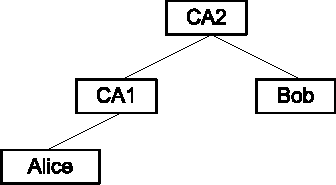
\includegraphics{Figures/pki/CA}
  \caption{Network of certificate authorities}
  \label{fig:cert authorities}
\end{figure}

Because Alice knows the public key of \emph{CA1}, she is able to
verify and willing to believe the public-key certificate for
\emph{CA2} signed by \emph{CA1}.  Such a certificate is sometimes
called a \mainindex{certificate!reverse certificate}\emph{reverse certificate},
because the signer is certifying a key for an entity higher up in the
hierarchy.  Once Alice deduces that $K_{CA2} \speaksfor \textrm{CA2}$,
she is able to verify and willing to believe the public-key
certificate for \emph{Bob} signed by \emph{CA2}.  This
certificate---in which the signer is certifying a key for an entity
lower in the hierarchy---is sometimes called a \mainindex{forward
  certificate}\emph{forward certificate}.

The following proof shows the trust assumptions made by Alice, as well as
the authorities she chooses to recognize: 

\begin{formalProof}
    1. $K_{CA1} \speaksfor \textrm{CA1}$ & trust assumption \\
    2. $K_{CA1} \says (K_{CA2} \speaksfor \textrm{CA2})$ & Key Certificate\\
    3. $K_{CA2} \says (K_{\name{Bob}} \speaksfor \textrm{Bob})$ & Key Certificate\\
    4. $\textrm{CA1} \controls (K_{CA2} \speaksfor \textrm{CA2})$ & Jurisdiction \\
    5. $\textrm{CA2} \controls (K_{\name{Bob}} \speaksfor \textrm{Bob})$ & Jurisdiction \\
    6. $\textrm{CA1} \says (K_{CA2} \speaksfor \textrm{CA2})$ & 1,2
    Derived Speaks For\\
    7. $K_{CA2} \speaksfor CA2$ & 4,6 Controls \\
    8. $\textrm{CA2} \says (K_{\name{Bob}} \speaksfor \textrm{Bob})$ &
    7, 3  Derived Speaks For \\
    9. $K_{\name{Bob}} \speaksfor \textrm{Bob}$ & 5,8  Controls
  \end{formalProof}

  The first line is Alice's belief that she knows the public key of
  \emph{CA1}. Lines two and three are the public-key certificates for
  \emph{CA2} (signed by \emph{CA1}) and \name{Bob} (signed by
  \emph{CA2}).  Lines four and five represent Alice's trust in
  \emph{CA1}'s reliability regarding certifying that $K_{CA2}$ is
  \emph{CA2}'s key, and in \emph{CA2}'s authority to say truthfully that
  $K_{\name{Bob}}$ is Bob's public key.  Lines six through nine are the
  steps necessary for Alice to deduce that $K_{\name{Bob}}$ is indeed
  Bob's public key.
\end{example}

% At this point we have developed the basic concepts of statements,
% certificates, proxies, and  jurisdiction of authority. From the
% standpoint of access control, we now have the basis for establishing who
% is making a request, under whose authority the request is being made,
% and credentials (certificates) to validate what is being said. %  In the
% % remaining sections we focus on basic access control mechanisms: tickets
% % and access-control lists.

\begin{exercise}[\appn]
  Suppose Toni sends Blake a message in the clear that is digitally
  signed as follows:
  \[(\textrm{`You're hired!''},
  \mathit{encrypt}(K^{-1}_{\name{Toni}},hash(\textrm{You're
    hired!''})))\] The above message is sent over an open channel, such
  as the Internet.  Laura intercepts the message and retransmits it to
  Blake with one crucial change: \emph{``You're hired!''} is changed to
  \emph{``You're fired!''}. Because she wants Blake to think that the
  message came from Toni, she reuses Toni's digital signature from the
  message she intercepted.

  What happens when Blake receives the message?  Is he able to detect
  the forgery or not?
\end{exercise}

\begin{exercise}[\appn]
  Use the \emph{Certificate Verification} rule to give an alternate
  proof for the situation in Example~\ref{ex:ca-chains}.
\end{exercise}

\begin{exercise}[\appn]
  This question relates to an online-purchase transaction, in which
  Zoey logs into a previously established account with her
  userid-password combination.  She then attempts to purchase an airline
  ticket, using her credit card.  In what follows, you should interpret
  $\mathit{CC}_Z$ as a principal representing a specific credit-card
  number/account.
  \begin{enumerate}
  \item Give English translations for each of the following statements,
    using notions such as \emph{authority} (or \emph{jurisdiction}),
    \emph{signatures}, \emph{sessions}, and \emph{access requests}.
%     Colloquial English is fine (and even preferred), provided your
%     translations accurately capture what's going on.

    \begin{enumerate}
    \item $\mathit{PwdServer} \controls
      (\pair{\texttt{zoey},\mathit{pwd}} \speaksfor \mathit{Zoey})$
    \item $\mathit{Visa} \controls ((\mathit{Zoey}\quoting
      \mathit{CC}_Z) \controls \mathit{buyticket})$
    \item $K_{P} \speaksfor \mathit{PwdServer}$
    \item $K_{V} \speaksfor \mathit{Visa}$
    \item $(\pair{\texttt{zoey},\mathit{pwd}}\quoting \mathit{CC}_Z)
      \says \mathit{buyticket}$
    \item $K_{P} \says (\pair{\texttt{zoey},\mathit{pwd}} \speaksfor
      \mathit{Zoey})$
    \item $K_{V} \says ((\mathit{Zoey}\quoting \mathit{CC}_Z) \controls
      \mathit{buyticket})$
    \end{enumerate}

  \item Give a formal proof that \textit{buyticket} can be deduced from
    the seven assumptions listed above.
  \end{enumerate}

\end{exercise}

\begin{exercise}[\synthesis]
  Dana has registered her public key $K_D$ with the certificate
  authority \name{CA}, whose public key is $K_\mathit{CA}$. She wishes
  to send a message $m$ to Earl, who does not know Dana and does not
  recognize the authority of \name{CA}.  Fortunately, Dana knows Earl's
  good friend Finn, who \emph{does} recognize \name{CA}'s authority.
  
  Furthermore, both Earl and Finn work at \name{Gaggle} and have
  registered their public keys ($K_E$ and $K_F$, respectively) with the
  company's certificate authority; the public key for \name{Gaggle}'s
  certificate authority is $K_G$.  (Note that both Earl and Finn have
  access to Gaggle certificates, but they have never exchanged their
  public keys with one another before.)

  Dana signs her message using her private key, and sends it to
  Finn.  She asks Finn to forward it to Earl, which Finn does as
  follows: 
  \begin{itemize}
  \item Finn uses his private key to sign Dana's signed message, and
    sends the result to Earl.
  \item Finn also gets a copy of Dana's public-key certificate, and
    signs and sends that to Earl.
  \item Finn signs a message that indicates what \name{CA}'s public
    key is, and sends that to Earl.
  \item Finally, Finn signs and sends to Earl a message stating his
    confidence in \name{CA}'s jurisdiction over Dana's public key.
  \end{itemize}

  \begin{enumerate}
  \item Express in the access-control logic the four items that Finn
    sends to Earl.
  \item Identify the additional certificates, recognitions of authority,
    and any other trust assumptions that Earl requires in order to
    deduce that the message $m$ truly came from \name{Dana}.  You
    should express each of these items in the access-control logic.
  \item Give a formal proof that $m$ can be deduced from your answers to
    parts~(a) and~(b).
  \item In your opinion, which if any of the assumptions from part~(b)
    are the most suspect?  Explain your answer.   

  \end{enumerate}
\end{exercise}
% % \chinbox{\textbf{At this point we need to say that PKI sets us up nicely
% %     to use access-control lists}}

\begin{exercise}[\synthesis]
  Two high-tech companies---\textsf{NanoTech} and
  \textsf{PicoWare}---are collaborating on a joint project called
  \textsc{Illumina}.  The project's repository and web page are housed
  at \textsf{PicoWare}'s facilities .

  When the two companies initiated this project, they established a
  special certificate authority (CA) that both companies would trust
  with respect to high-level company keys \emph{for the purposes of this
    project} only.   The public-private key pairs for the various
  entities are as follows: 

  \begin{center}
  \begin{tabular}{cl}
    $(K_{CA},K^{-1}_{CA})$ &  CA's key pair, trusted by both companies
    \\
    $(K_{N},K^{-1}_{N})$ &  \textsf{NanoTech}'s key pair, with $K_N$ registered
    with $CA$ \\
    $(K_{P},K^{-1}_{P})$ &  \textsf{PicoWare}'s key pair, with $K_P$ registered
    with $CA$ 
  \end{tabular}
  \end{center}
  This setup allows both \textsf{NanoTech} and \textsf{PicoWare} to maintain
  their existing company key infrastructures, and neither company has to
  blindly trust the other's infrastructure.  Specifically:
  \begin{itemize}
  \item \textsf{NanoTech}'s public key has been installed on all machines at
    \textsf{NanoTech}; therefore \textsf{NanoTech} machines do not need to
    fetch \textsf{NanoTech}'s 
    certificate from CA. 
  \item Likewise, \textsf{PicoWare}'s public key has been installed on all
    machines at \textsf{PicoWare}; therefore \textsf{PicoWare} machines do
    not need to fetch
    \textsf{PicoWare}'s certificate from CA.
  \item Neither company's public key has been installed on any of the
    other company's machines.  Therefore, certificates from CA are
    necessary for any secure cross-company communication.
  \item Each company certifies its own internal keys: the keys for all
    \textsf{NanoTech} employees and \textsf{NanoTech} machines are
    certified by \textsf{NanoTech}, and the keys for all
    \textsf{PicoWare} employees and \textsf{PicoWare} machines are
    certified by \textsf{PicoWare}.
  \end{itemize}

%  \textbf{Your task:} Answer the following series of questions.

  \begin{list}{(\alph{count})}{\usecounter{count}}
  \item The access-control policy for the \textsc{Illumina} project web
    page grants \textbf{both} read access (\action{\mathit{read, iwp}})
    and write access (\action{\mathit{write, iwp}}) to all members of the
    \textsc{Illumina} project.  Express this access-control policy as an
    expression in the access-control logic.  % (\emph{Note:} You do not
%     have to preface this statement with ``$\textit{ACL} \says
%     \cdots$''.)  \vspace*{1in}

  \item Stan---a \textsf{NanoTech} employee---has been issued the key pair
    $(K_S,K^{-1}_S)$.  Express Stan's public-key 
    certificate as an expression in the access-control logic.

  \item Stan has been assigned to the \textsc{Illumina} project team, and
    the group database at \textsf{PicoWare} has been updated to reflect
    this group membership.  If ever requested, the group-database server
    (GDS) can digitally sign a statement that attests to Stan's group
    membership; the group-database server's key pair is $(K_{GDS},
    K_{GDS}^{-1})$.

    Express such a certificate as an expression in the access-control
    logic.  
    \setcounter{restart}{\thecount}
  \end{list}

  Stan logs into his \textsf{NanoTech} office computer, using his
  \textsf{NanoTech}-issued smart card.  He then tries to establish an
  SSL connection to the \textsc{Illumina web page} at \textsf{PicoWare}.
  To authenticate the SSL connection, Stan's smart card uses his private
  key to cryptographically sign a response to a challenge from the
  \textsf{PicoWare} server.  The SSL connection is secured with a
  session key $K_{ssl}$.  From the point of view of the web server at
  \textsf{PicoWare}, the result of successfully establishing this SSL
  connection is the following trust assumption:
  \[ K_{ssl} \speaksfor K_{S}  \qquad (\ast) \]

  \begin{list}{(\alph{count})}%
    {\usecounter{count}\addtocounter{count}{\therestart}}%
  \item \textsf{PicoWare}'s web server receives (via SSL) Stan's request
    to read the \textsc{Illumina} web page.  Express this request as an
    expression in the access-control logic.  
  \item What are the additional certificates,
      recognition of authority, and trust assumptions regarding keys
    that are necessary for the \textsf{PicoWare} web server to determine that
    the read request should be granted? %
  \item Give a formal proof that justifies granting the request.
    Your only assumptions should be your answers to (a) through (e),
    plus the trust assumption ($\ast$).  
  \end{list}
\end{exercise}

\begin{exercise}[\synthesis]
  Some access-control decisions are made based on \emph{attributes}
  (properties such as one's age or the amount of money in your checking
  account) rather than \emph{identity}.  For example, consider what
  happens when you use a fare card like the Metro card in Washington,
  D.C.'s Metro system:
  \begin{itemize}
  \item From the standpoint of the rider, there are two resources to be
    accessed: the train at the starting destination and the exit to the
    street at the
    ending destination.

  \item The Metro card is a certificate issued by the individual Metro
    stations and possessed by the rider. Note, however, that while the
    \emph{physical card} may be the same before entering and after
    leaving the Metro station, it is \textbf{not} the same certificate:
    \begin{itemize}
    \item The information on the Metro card (particularly the amount of
      money left on the card) must be updated.
    \item The authorities that sign or vouch for the amount on the card
      are different: the turnstile used at the beginning of a rider's
      trip is different from the turnstile used at the end of the trip.
      Distinguishing the separate turnstiles (more accurately, the
      different stations) permits one to charge different amounts for
      different trips: the exit turnstile can always determine where the
      trip originated and how much to deduct from the card.
    \end{itemize}
  \end{itemize}

  To see how this works, consider a rider who wishes to travel from
  \name{Station A} to \name{Station B}, which is a trip that costs
  \$1.  Let's assume that the rider's most recent exit was at
  \name{Station C}, with a balance of \$5 on the card.
  \begin{itemize}
  \item The rider inserts the Metro card into the turnstile at
    \name{Station A}.  This card is (ultimately) interpreted as:
    \[ \name{Station C} \says (\name{balance=\$5} \wedge \name{exit=
      Station C}). \]
    Because the balance is greater than \$0, access to the train is
    granted; the card is returned to the rider saying (in effect): 
    \[ \name{Station A} \says (\name{balance=\$5} \wedge \name{entry=
      Station A}). \]
  
  \item The rider boards the train and travels to \name{Station B}.

  \item The rider inserts his or her Metro card into the turnstile at
    \name{Station B}.  Because the balance is sufficient to cover the
    cost of the trip, the turnstile returns the Metro card with an
    updated balance of \$4.
  \end{itemize}

  Assume that the turnstiles at the three stations ($A$, $B$, and $C$)
  form a private network called \name{MetroNet}.  There is a single
  certification authority \name{CA} that issues public/private key pairs
  and certifies membership in \name{MetroNet}.    The relevant
  keys are as follows:
  \begin{center}
  \begin{tabular}{cl}
    $(K_{CA},K^{-1}_{CA})$ &  CA's key pair    \\
    $(K_{A},K^{-1}_{A})$ &  \name{Station A}'s key pair    \\
    $(K_{B},K^{-1}_{B})$ &  \name{Station B}'s key pair    \\
    $(K_{C},K^{-1}_{C})$ &  \name{Station C}'s key pair 
  \end{tabular}
  \end{center}
  Digital signatures
  (based on the public and private keys distributed by the \name{CA})
  are used to provide protection against fraudulent cards.  Thus, the
  fare cards are actually digitally signed certificates.

  Use expressions in the access-control logic to answer the following
  questions regarding the certifications, credentials, and
  access-control policies needed for a rider to travel from
  \name{Station A} to \name{Station B}.
  %
  Treat attributes such as ``$\name{balance=\$5}$,''
  ``$\name{balance} > \$0$,'' and ``\name{exit= Station C}'' as simple
  propositions. Use \action{\name{enter,A}} and \action{\name{exit,B}}
  to denote entering at \name{Station A} and leaving at \name{Station
    B}, respectively.

  \begin{enumerate}
  \item  What are the necessary certificates,
      recognition of authority, and trust assumptions about keys for a
    turnstile at \name{Station B} to recognize \name{Station A} as
    belonging to \name{MetroNet}? 

  \item What are the necessary certificates,
      recognition of authority, and trust assumptions about keys for a
    turnstile at \name{Station B} to interpret an arbitrary fare card
    signed by \name{Station A}?  

  \item  What is the access policy of turnstiles at
    \name{Station A} that guard entry to trains?

  \item Assuming that a turnstile at \name{Station A} grants entry
    access to a rider, what certificate is given back to the rider as he
    or she passes through the turnstile?

  \item Assuming that a turnstile at \name{Station B} allows
    a rider to exit, what certificate is given back to the rider as he
    or she passes through the turnstile? 
  \end{enumerate}

\end{exercise}

\section{Symmetric-Key Cryptography}

\mainindex{cryptography!symmetric-key cryptography}As mentioned earlier in this
chapter, an alternative to public-key cryptography is
\mainindex{cryptography!shared key} \emph{shared-key} cryptography, also known as
\emph{symmetric-key cryptography} because the same key is used for
both encryption and decryption.  If \emph{encrypt} and \emph{decrypt}
are particular symmetric-key encryption and decryption functions, then
the following property must hold for all messages $m$ and keys $K$:
\[ \mathit{decrypt}(K,\mathit{encrypt}(K,m))  =  m. \]

\mainindex{cryptography!symmetric-key cryptography!compared with asymmetric-key
  cryptography}\mainindex{cryptography!asymmetric-key cryptography!compared with
  symmetric-key cryptography}Symmetric-key encryption
algorithms---such as the Advanced Encryption Standard (AES)
\cite{AES}---provide a significant advantage over public-key
algorithms in terms of efficiency.  They are typically three orders of
magnitude faster than public-key algorithms, because of the underlying
operations they employ (i.e., exclusive-or and bit substitutions as
opposed to modulo-$n$ exponentiation).  For this reason, it is often
preferable to encrypt large messages or files using symmetric-key
cryptography.

However, shared-key cryptography also has disadvantages that arise
from its use of a single key.  The first problem is one of planning:
Alice can send a secure message to Bob \emph{only} if they have
previously agreed upon a specific key to use.  Such an arrangement
should happen via out-of-band communication, such as during a
face-to-face meeting or some other reasonably secure means.  In
contrast, Alice can send a secure message to Bob via public-key
cryptography even if they have never communicated before, as long as
they have both published their public keys.

Another problem with shared-key cryptography is one of scale: each
principal must maintain a separate key for every other principal with
whom he or she wishes to communicate.  Thus, a collection of $n$
principals would require on the order of $n^2$ keys to support all
possible two-way conversations; public-key cryptography would require
only $2n$ keys (i.e., public and private keys for each principal). 

Finally, shared-key cryptography does not support the separation of
privacy and authenticity concerns.  For example, suppose that Alice
wishes to publish a message (i.e., allow it to be read by anyone) in a
way that provides evidence of her authorship.  We have already seen how
to accomplish this goal using public-key cryptography.  However,
symmetric-key cryptography does not support this goal directly: anyone who has
knowledge of the key to decrypt the message could forge a new message or
even claim to be the original author.

These disadvantages can be somewhat mitigated through the use of
\emph{relays} to simulate a public-key infrastructure.  We demonstrate
how later in Examples~\ref{ex:relays} and~\ref{ex:relays-auth}, but we
must first address one additional pragmatic difference between
public-key and shared-key cryptography.  A sender using public-key
cryptography can tell the recipient the relevant key to use.  For
example, if Alice sends a digitally signed message to Bob, she can also
send along her public key for his convenience.  Likewise, if she sends a
secret message to Bob using his public key, she can notify him which
public key she used; that information is useless to anyone who does not
know Bob's private key.

If Alice instead uses shared-key cryptography, then she obviously
cannot directly indicate which key Bob should use to decrypt the
message.  However, she can accomplish the same goal by sending along a
\emph{key identifier} (or \mainindex{cryptography!key hint}\emph{key hint}) that
will be meaningful only to Bob.  A \mainindex{cryptography!key identifier}key
identifier might be as simple as an index into a table of keys that is
kept on Bob's machine.  Alternatively, Bob may have a master key that
he uses to encrypt all his other keys: the key identifier for a shared
key $K$ may be the result of encrypting $K$ with that master key.  The
point here is that, when Alice and Bob set up their shared key, they
must also have exchanged their individual key identifiers associated
with that key.  However, neither needs to know \emph{how} the other
selects their key identifiers.  The following example demonstrates the
use of key identifiers.

\begin{example}\label{ex:key-hints}
  Both Richard and Janet use master keys ($K_R$ and $K_J$, respectively)
  to encrypt all their important keys.  They have recently set up a
  shared key $K_S$ that will allow them to communicate with one another
  securely.  At that time, they also exchanged key identifiers:
  \begin{itemize}
  \item Richard keeps a table of encrypted keys on his computer, and he
    likes to use the indices of this table as his key identifiers.  Richard
    adds the encrypted shared key (i.e., $\mathit{encrypt}(K_R,K_S)$) to
    this table, and gives the corresponding index (e.g., $213$) to Janet as
    the key identifier to use for this key.
  \item Janet prefers to use encrypted keys themselves as key identifiers.
    She therefore encrypts the shared key with her master key and gives
    the result to Richard as \emph{her} key identifier for the key:
    $\mathit{encrypt}(K_J,K_S)$.
  \end{itemize}

  When Janet sends a secure message to Richard using the shared key
  $K_S$, she also sends him his 
  key identifier (i.e., $213$) for the key.  Richard is able to look up the
  appropriate entry in his table (i.e., $\mathit{encrypt}(K_R,K_S)$),
  decrypt it with his master 
  key $K_R$ to obtain $K_S$, and then use $K_S$ to decrypt Janet's
  message.  

  Similarly, when Richard sends a secure message to Janet using the
  shared key $K_S$, he also includes her key identifier (i.e.,
  $\mathit{encrypt}(K_J,K_S)$).  Janet knows to decrypt this hint with
  her master key $K_J$ to obtain the key necessary to decrypt Richard's
  message.
\end{example}

As the preceding example shows, two principals may have very different
key identifiers for the same shared key.  What is important is that each
knows the other's key identifier for the shared key, so that they can
always clearly communicate which key is being used.  (In fact, two
principals may share multiple keys, using each for a different purpose.
The use of key identifiers allows them to indicate which is relevant for
the given communication.)

We adopt the notational convention\footnote{For convenience, we often
  blur the distinction between keys and key identifiers when using the
  logic.  The important point of this discussion is that key hints can
  be used both in practice and in the logic to shroud secret keys.} of
using principals' names or initials as superscripts on keys to denote
a given principal's key hint for a specific key.  For example, we use
\mainindex{cryptography!key hint!notational convention}$K_{S}^{R}$ and
$K_{S}^{J}$ to denote Richard's and Janet's key hints for the shared
key $K_S$.  We can then associate the key hints with the statements
that they make (i.e., with the messages encrypted by the keys they
hint at).  Thus, if Janet sends Richard the message $m$ encrypted with
the shared key $K_s$, we can express Richard's interpretation as
follows:
\[ K_{S}^{R} \says m. \]
If Richard trusts Janet to keep the shared key $K_S$ private, then he
should be willing to associate messages encrypted by $K_S$ with Janet.
That is, he should be willing to view the key hint
$K_{S}^{R}$ (and the key it represents) as a proxy for
Janet:
\[ K_{S}^{R} \speaksfor \name{Janet}. \]




% \begin{itemize}
% % \item Trust: Both Alice and Bob must trust each other to keep key secret.  (Is
% %   this really different from public-key case?)
% \item Planning: Alice and Bob must set up specific key prior to use
%   using out-of-band communication.  (What about data-encryption keys?)
% \item Scale: Given $n$ principals, it requires $O(n^2)$ rather than
%   $O(n)$ keys.
% \item Cannot separate privacy from authenticity: instead, must rely on
%   others to protect secrecy of key.
% \end{itemize}


The following series of examples, inspired by a discussion in
\cite{LABW}, demonstrates how a symmetric-key system can mimic a
public-key infrastructure by judicious use of key identifiers.  The
approach hinges on the use of
\mainindex{cryptography!relays}\emph{relays}, trusted agents that serve
as encryption/decryption intermediaries.  Just as any principal can
register a public-key with a certificate authority in a PKI,
\mainindex{cryptography!relays!use of to mimic PKI}the relay system
requires that any principal $Q$ be able to register with a special
trusted agent.  Furthermore, the trusted agent must know the relay's
master key, which the relay uses for creating its
\mainindex{cryptography!key hint!use with relays}key identifiers
(similar to Janet's method for key identifiers in
Example~\ref{ex:key-hints}).
% Each
% principal $P$ that 
% wishes to use the relay $R$ must share a secret key $K_P$ (plus the key
% hints  with the relay

\begin{example}\label{ex:relays}
  Quinton wishes to use symmetric encryption to send a message that
  Shelby can read and verify as being from Quinton.  Although Shelby
  and Quinton do not share a key, they have both previously
  established secret-key channels with the trusted relay $R$ by
  registering with a trusted agent $TA$.  When Quinton registered,
  $TA$ created and sent back to Quinton two items:
  \begin{enumerate}
  \item A secret key $K_q$ to be shared between Quinton and the relay
    $R$
  \item $R$'s key identifier $K_q^R = \encrypt{K_q}{K_m}$ for this key,
    which $TA$ creates by encrypting the new key $K_q$ with $R$'s master
    key $K_m$
  \end{enumerate}
  $TA$ also publishes a \mainindex{certificate!secret-key
    certificate}\emph{secret-key certificate} for Quinton that
  contains two components
  \symindex{$<\negthickspace\negthickspace<m_1,m_2,\ldots,
    m_k>\negthickspace\negthickspace>$: concatenation}(we introduce the
  notation \cat{m_1,m_2,\ldots, m_k} to denote the concatenation of
  the $k$ items $m_1$ through $m_k$):
  \[ \encrypt{\cat{K_q^Q,K_q^R,\name{Quinton}}}{K_{ta}}, \quad
  K_{ta}^R. \]
  The first item associates the pair $(K_q^Q, K_q^R)$ of key identifiers
  with Quinton; this item is signed by $TA$ using the key $K_{ta}$ that
  it shares with the relay.  The second item is the relay's key hint for
  the shared key $K_{ta}$, so that anyone who wishes to read the
  certificate can direct the relay which key to use for decryption.
%   \item Quinton's \emph{shared-key certificate}, signed with the key
%     that $TA$ shares with $R$ ($K_{ta}$) and combined with the
%     appropriate key hint for this key ($K_{ta}^R$):
%     \[ \encrypt{\cat{K_q^Q,K_q^R,\name{Quinton}}}{K_{ta}}, \qquad
%     K_{ta}^R \]
  Unlike a public-key certificate, the shared-key certificate
  is not readable by just anybody: only a principal that knows the
  secret key $K_{ta}$ (such as $TA$ and the relay) can read it.

%   $TA$ gave both the key and
%   $R$'s key identifier to Quinton, who is able to construct his own key
%   identifier $K_q^Q$ for the key.  In a similar fashion, Shelby shares a
%   key $K_s$ with the relay and knows the relay's key identifer $K_s^R$
%   for that key.

  Quinton encrypts his message $m$ with the key $K_q$, sending both the
  encrypted message and the key hint $K_q^R$ to Shelby:
  \[ \encrypt{m}{K_q}, \quad K_q^R. \] Shelby cannot decrypt the message
  directly, because she does not know the shared key that $K_q^R$
  identifies.  However, 
  because Shelby also registered with $TA$, she shares a secret key
  $K_s$ with the relay and knows the relay's key hint $K_s^R$ for that
  key.  She therefore forwards these items on to the relay $R$, along
  with the key-identifier pair $(K_s^S,K_s^R)$.  In effect, Shelby is
  requesting a decryption of the encryption message and telling the
  relay how to return the answer.  (Shelby can also forward on Quinton's
  shared-key certificate for decryption, if she wishes to authenticate
  the message.  We leave this possibility for Example~\ref{ex:relays-auth}.) 

  The relay applies its master key $K_m$ to the key hint $K_q^R$ to
  obtain the key $K_q$:
  \[ \mathit{decrypt}(K_m, K_q^R) = \mathit{decrypt}(K_m,
  \encrypt{K_q}{K_m}) = K_q. \] 
  With this key, the relay can decrypt the message \encrypt{m}{K_q} to
  obtain the original message $m$:
  \[ \mathit{decrypt}(K_q, \encrypt{m}{K_q}) = m . \] 
  The relay then repackages this message for Shelby by encrypting $m$
  with the shared key $K_s = \mathit{decrypt}(K_m, K_s^R)$, sending back
  the newly encrypted version as well as the key hint $K_s^S$:
  \[ \encrypt{m}{K_s}, \quad K_s^S. \]

  Upon receiving this package, Shelby uses the key hint $K_s^S$ to
  identify the correct key ($K_s$) to use to decrypt the message:
  \[ \mathit{decrypt}(K_s, \encrypt{m}{K_s}) = m.  \]
  As a result of this process, Shelby interprets this message as follows:
  \[ K_s^S \says K_q^R \says m. \]
  That is, the key identifier $K_s^S$ is claiming that the key hint
  $K_q^R$ was used to send the message $m$.  If Shelby trusts the relay
  to keep the key $K_s$ secret (i.e., if she believes that $K_s^S
  \speaksfor R$) and to accurately translate messages (i.e., $R
  \controls K_q^R \says m$), then she will deduce that $m$ was the
  original intended message she received (i.e., $K_q^R \says m$).
\end{example}

The previous example demonstrated how secret-key cryptography can be
used to exchange messages between principals who have not previously
established a shared secret key.  However, the example as it stands does
not address authentication concerns: neither the relay nor Shelby are
able to associate the key identifier $K_q^R$ with Quinton at the end of
the process described.  To do so, they must also make use of Quinton's
secret-key certificate as demonstrated in the next example. 


\begin{example}\label{ex:relays-auth}
%   Recall from the previous example that the trusted authority $TA$ knows
%   the relay's master key and can therefore always calculate the relay's
%   key identifier for any given secret key.  When Quinton initially
%   registers with $TA$, $TA$ publishes a secret-key certificate containing the
%   following two components:
%   \[ \encrypt{\cat{K_q^Q,K_q^R,\mathit{Quinton}}}{K_{ta}}, \quad
%   K_{ta}^R. \]
%   The first item associates the pair $(K_q^Q, K_q^R)$ of key identifiers
%   with Quinton; this item is signed by $TA$ using the key $K_{ta}$ that
%   it shares with the relay.  The second item is the relay's key hint for
%   the shared key $K_{ta}$, so that anyone who wishes to read the
%   certificate can direct the relay which key to use for decryption.
  By the end of Example~\ref{ex:relays}, Shelby had deduced that $K_q^R
  \says m$.  If she wishes to authenticate Quinton as the message's author
  (i.e., to associate the key hint $K_q^R$ with Quinton), then she
  forwards Quinton's secret-key certificate to the relay along with her
  key-hint pair $(K_s^S,K_s^R)$.  As with the original message, the
  relay can decrypt the certificate, 
  which can be expressed in the logic as follows:
  \[ K_{ta}^R \says ((K_q^Q, K_q^R) \speaksfor \name{Quinton}). \]
  That is, the key hint $K_{ta}^R$ claims that the key-hint pair
  $(K_q^Q, K_q^R)$ is associated with Quinton.  If the relay trusts that
  the key hint $K_{ta}^R$ (i.e., the key $K_{ta}$) represents $TA$ and
  that $TA$ has jurisdiction over which keys represent which principals,
  then it will be able to associate the key hint $K_q^R$ with
  $\name{Quinton}$.

  At this point, the relay must create for Shelby a new certificate that
  associates the key hint $K_q^R$ with Quinton.  The relay sends the
  following items to Shelby:
  \[ \encrypt{\cat{K_q^R,\name{Quinton}}}{K_s}, \quad K_s^S. \] 
  As before, Shelby can decrypt the message to interpret the certificate
  as follows:
  \[ K_s^S \says (K_q^R \speaksfor \name{Quinton}). \]
\end{example}

As a final twist on this scenario, suppose that Shelby wishes to
exchange a series of messages with Quinton.  She may wish to set up
an authenticated channel between herself and Quinton, so that they can
exchange messages directly without having to use the relay for continual
translations.   As the following example demonstrates, Shelby can enlist
the relay's help to set up such a channel. 

\begin{example}\label{ex:relays-auth-channel}
  To set up an authenticated channel with Quinton, Shelby proceeds in
  the same way as at the beginning of Example~\ref{ex:relays-auth}.  
  She
  forwards Quinton's secret-key certificate to the relay along with her
  key-hint pair $(K_s^S,K_s^R)$.  The relay decrypts this certificate
  and interprets it as before:
  \[ K_{ta}^R \says ((K_q^Q, K_q^R) \speaksfor \name{Quinton}). \]
%   That is, the key hint $K_{ta}^R$ claims that the key-hint pair
%   $(K_q^Q, K_q^R)$ is associated with Quinton.  If the relay trusts that
%   the key hint $K_{ta}^R$ (i.e., the key $K_{ta}$) represents $TA$ and
%   that $TA$ has jurisdiction over which keys represent which principals,
%   then it will be able to associate the key hint $K_q^R$ with
%   $\name{Quinton}$.

  The relay now creates a new channel for direct
  communication between Quinton and Shelby.  Specifically, the relay
  creates a new key $K$ and creates key identifiers for Quinton and
  Shelby by encrypting it with their individual keys:
  \[ K^Q = \encrypt{K}{K_q}, \qquad K^S = \encrypt{K}{K_s}. \]
  The relay then creates a new certificate for Shelby that associates
  this new key-hint pair $(K^Q,K^S)$ with Quinton:
  \[ \encrypt{\cat{K^Q,K^S,\name{Quinton}}}{K_s}, \quad
  K_s^S. \]
  Shelby can interpret this certificate as follows:
  \[ K_s^S \says ((K^Q, K^S) \speaksfor \name{Quinton}). \] 
  (If Quinton wishes to also authenticate Shelby, then the relay will
  need to obtain Shelby's original secret-key certificate and then
  generate a new one for Quinton to use in a similar fashion.)
\end{example}

\begin{exercise}[\eval]Consider the certificate that Shelby receives at
  the end of   Example~\ref{ex:relays-auth}.
  \begin{enumerate}
  \item What additional trust assumptions must Shelby make in order to
    identify Quinton as the sender of the original message from
    Example~\ref{ex:relays}?
  \item Another possible interpretation in the logic of that certificate
    is as follows:
    \[ K_s^S \says (K_s^S \quoting K_q^R \speaksfor \name{Quinton}). \]
    Given this interpretation, what additional trust assumptions must
    Shelby make in order to identify Quinton as the sender of the
    original message from Example~\ref{ex:relays}?
  \item Briefly describe the advantages and disadvantages of the two
    interpretations, and identify the situations where each might be
    more appropriate.
  \end{enumerate}


\end{exercise}

\begin{exercise}[\appn]
  What additional trust assumptions must Shelby make to associate the
  new key $K$ (or its associated key-hint pair) with Quinton in
  Example~\ref{ex:relays-auth-channel}? 
\end{exercise}

\begin{exercise}[\synthesis]
  Suppose that two-way authentication is necessary in
  Example~\ref{ex:relays-auth-channel} (i.e., Quinton also wishes to
  authenticate Shelby).
  \begin{enumerate}
  \item What messages need to be sent between Quinton and the relay?
  \item Express in the access-control logic how these messages are
    interpreted, along with the trust assumptions necessary for the
    protocol to succeed.
  \end{enumerate}
\end{exercise}



% \begin{exercise}[\synthesis]
%   Kerberos is a protocol that provides secure authentication for
%   principals on an insecure network, using symmetric (i.e., shared-key)
%   encryption.  In a nutshell, here's how Kerberos works:
%   \begin{description}
%   \item[(1)] A user Claude logs into his workstation, and enters his
%     password.  A program running on the workstation (i.e., the
%     \emph{client}) does two things: (1) it sends unencrypted the user's
%     name to the \emph{Authentication Server (AS)}, and (2) it runs a
%     predetermined one-way hash function on Claude's password to
%     create the \emph{client's secret key} ($K_{C}$).  (Note: By
%     generating this key fresh, the workstation does not need to store it
%     when Claude is not logged in.  However, the same key will have been
%     previously stored by the AS.)
%   \item[(2)] The AS looks Claude's username up in its database, to ensure that
%     Claude is an authorized user.  Along with the listing for Claude is Claude's
%     secret key $K_C$.  The AS sends two items back to the client:
%     \begin{itemize}
%     \item A newly generated \emph{session key} $K_{c,tgs}$ through which
%       the client can communicate with the \emph{ticket-granting server
%         (TGS)}; this key is encrypted with the client's secret key $K_C$.
%     \item A ticket that associates the session key $K_{c,tgs}$ with the
%       client (including the client's id and network address, a ticket validity
%       period, etc); this ticket is encrypted with the key $K_{TGS}$,
%       which is shared by AS and TGS.
%     \end{itemize}
%   \item[(3)] Now, when Claude wants to (say) print a file, he needs to 
%     authenticate to the \emph{Print Server (PS)}; to do so, he must 
%     first get a ticket from the TGS.  Therefore, the client on Claude's
%     behalf sends the following three items to TGS:
%     \begin{itemize}
%     \item The name of the server it wishes to authenticate to (in this
%       case, \name{PS}) 
%     \item The ticket that AS had sent to the client on the previous step
%       (i.e., the one encrypted with $K_{TGS}$)
%     \item An \emph{authenticator}, which is a message that contains the
%       client's id and is encrypted with the session key $K_{c,tgs}$
%     \end{itemize}
%   \item[(4)] The TGS uses its secret key $K_{TGS}$ to decrypt the ticket,
%     after which it can use the session key $K_{c,tgs}$ to decrypt the
%     authenticator and verify that the client making the request is the
%     one authorized by AS to do so.  Assuming everything checks out, the
%     TGS sends a new ticket to the client that can be used to request
%     services from the Print Server.
%   \end{description}
%   The Kerberos protocol continues for a few more steps, but this
%   question concerns only the decision made in Stage~4 described above.
% %   The three items that the client sends to the TGS in Stage~3 can be
% %   interpreted as statements in the logic as follows:
% %   \begin{itemize}
% %   \item The name of the server it wishes to authenticate to (in this
% %     case, \name{PS}) 
% %     \[ \name{client@address} \says \action{\name{get ticket,PS}} \]
% %   \item The ticket that AS had sent to the client on the previous step
% %     (i.e., the one encrypted with $K_{TGS}$)

% % %    \[ K_{TGS} \says (K_{c,tgs} \speaksfor \name{client@address}) \]
% %     \[ K_{TGS} \says (K_{c,tgs} \controls (\name{client@address}
% %     \controls \action{\name{get ticket, PS}}))  \]
% %   \item An \emph{authenticator}, which is a message that contains the
% %     client's id and is encrypted with the session key $K_{c,tgs}$

% %     \[ K_{c,tgs} \says (\name{client@address} \controls
% %     \action{\name{get ticket,PS}}) \] 
% %   \end{itemize}
% %   \textsc{Important note:} \emph{In lecture, we discussed how pairs of
% %     key identifiers can be used to name shared-key encryption channels.
% %     To keep the notation simple in this question, I am using the shared
% %     keys directly to name the channels.}


%   Consider an analysis of this situation from the point of view
%   of the \textbf{ticket-granting server (TGS)}, as it determines whether
%   or not to grant the requested ticket.
%   Specifically, the three items that the client sends to the TGS in
%   Stage~3 can be interpreted as statements in the logic as follows:
%   \begin{itemize}
%   \item The name of the server it wishes to authenticate to (in this
%     case, \name{PS}) 
%     \[ \name{client@address} \says \action{\name{get ticket,PS}} \]
%   \item The ticket that AS had sent to the client on the previous step
%     (i.e., the one encrypted with $K_{TGS}$)

% %    \[ K_{TGS} \says (K_{c,tgs} \speaksfor \name{client@address}) \]
%     \[ K_{TGS} \says (K_{c,tgs} \controls (\name{client@address}
%     \controls \action{\name{get ticket, PS}}))  \]
%   \item An \emph{authenticator}, which is a message that contains the
%     client's id and is encrypted with the session key $K_{c,tgs}$

%     \[ K_{c,tgs} \says (\name{client@address} \controls
%     \action{\name{get ticket,PS}}) \] 
%   \end{itemize}
%   \textsc{Important note:} \emph{In lecture, we discussed how pairs of
%     key identifiers can be used to name shared-key encryption channels.
%     To keep the notation simple in this question, I am using the shared
%     keys directly to name the channels.}

%   \begin{enumerate}
%   \item The TGS must recognize the jurisdiction of one or
%     more authorities, and make one or more additional trust assumptions,
%     in order to grant the ticket: what are they?  Express your answers
%     as statements in the access-control logic. 
%   \item Give a formal proof that the request can be granted,
%     using as your only assumptions the three statements given above
%     plus your answers to Part~(2).
%   \end{enumerate}

% \end{exercise}


\section{Summary}

We have already seen that authentication---that is, identifying the
originator of a request---is critical to sound access control.  In the
digital world, authentication is made more difficult by the physical
absence of the requesting principal: a request arrives as a sequence of
bits, with only hints of its origin.  

In this chapter, we saw how public-key infrastructures support digital
authentication through the use of public and private keys, digital
signatures, public-key certificates, and certificate authorities.  A PKI
supports integrity, privacy, and authentication by providing the means
to associate specific keys---and, subsequently, specific
statements---with specific principals.  We explored how to express and
reason about the fundamental concepts of PKI in the access-control
logic. We also discussed the main differences between symmetric
and asymmetric cryptography.

The learning outcomes associated with this chapter appear in
Figure~\ref{fig:outcomes-chap6}.

\begin{figure}[tb]
  \centering
After completing this chapter, you should be able to achieve the following
learning outcomes at several levels of knowledge:
\begin{description}
\item[Comprehension] \
  \begin{itemize}
  \item Describe the characteristics of private-key and secret-key
    cryptographic systems.
  \item Describe basic principles of trust topologies and networks of
    certification authorities.
  \end{itemize}
\item[Application] \
  \begin{itemize}
  \item When given protocol descriptions and trust hierarchies, you
    should be able to use the access-control logic to describe the
    protocol and trust relationships.
  \item When given a trust topology, you should be able to determine the
    necessary certificates for establishing trust in a key.
  \end{itemize}
\item[Analysis] \
  \begin{itemize}
  \item When given a set of certificates, you should be able to formally
    derive whether a key is associated with a particular principal.
  \end{itemize}
\item[Synthesis] \
  \begin{itemize}
  \item When given a description of a trust topology, you should be able
    to create a formal description of the certificates and trust
    relationships for the certification authorities.
  \end{itemize}
\end{description}
  
  \caption{Learning outcomes for Chapter~6}
  \label{fig:outcomes-chap6}
\end{figure}

\section{Further Reading}
The \emph{Handbook of Applied Cryptography} \cite{Handbook} is a very
mathematical and authoritative reference for cryptographic algorithms,
hash algorithms, digital signatures, and cryptographic protocols.
William Stallings' book \emph{Cryptography and Network Security
  Principles and Practices} \cite{Stallings} is a less comprehensive but
more accessible reference.

% ---- this points LaTeX to book.tex ----
%%% Local Variables:
%%% TeX-master: "book"
%%% End:

%  LocalWords:  PKI RSA cryptosystem checksum AES dek plaintext Zoey
%  LocalWords:  GoodBooks TrueSignatures online userid PwdServer zoey
%  LocalWords:  pwd buyticket NanoTech PicoWare Illumina other's iwp
%  LocalWords:  GDS SSL ssl one's MetroNet indices getMessage deciphS
%  LocalWords:  Accessor datatype msg SymKey symMsg sym num deciphP
%  LocalWords:  pKey asymMsg princ pubK privK signVerify signVerifyOK
%  LocalWords:  Stallings


\chapter{Reasoning about Transitions}
\label{chap:transitions}

% ---- this points LaTeX to book.tex ---- 
% Local Variables: 
% TeX-master: "book"
% End:


\chapter{Reasoning Using the Higher Order Logic Theorem Prover\\
\small{\redtext{\textsc{Do Not Distribute}}}}
\label{chap:hol}

% \chinbox{
%   \begin{itemize}
%   \item HOL as a CAD tool
%   \item HOL is stable
%   \item Chapter meant to provide reading knowledge, not a user's manual
%   \item Distinction between meta and object levels
%   \end{itemize}
% }

\paragraph*{Why Use Theorem Provers?}

Human error is ever present in even the simplest of calculations. As
security and integrity are crucial to critical applications such as
command-and-control, and designs have a myriad of detail, the chances
of getting every detail absolutely correct is vanishingly
small. 

The need to handle a large number of design and verification details
is not new. This is the same situation faced by design and
verification engineers of very large-scale integrated (VLSI)
circuits. Modern microprocessors have billions of transistors. Even
the simple-sounding task of accounting for all the connections among a
microprocessor's transistors is completely impractical using manual
methods alone. Computer-assisted design (CAD) tools for design-rule
checking (checking to make sure that circuit layouts satisfy rules
such as minimum width and spacing constraints between wires) and logic
to layout verification (checking that the electrical behavior of
transistor-level circuits is consistent with the logical behavior
described by logic schematics), are essential for VLSI hardware
design.

Assuring system security and integrity requires consistency among
policies and implementations across multiple levels of abstraction:
from high-level organizational policies down to the control of
physical memory. Managing and guaranteeing consistency among
access-control policies, trust assumptions, and interpretation of
messages and certificates is beyond manual methods.

Computer-assisted reasoning tools, such as proof checkers and theorem
provers, for checking consistency among policies and implementations,
have an analogous role to CAD tools in hardware design. Both are
antidotes to human error, self-delusion, and the complexity of large
numbers of design details. 

There are several advantages to using theorem provers and proof checkers.
\begin{enumerate}
\item Formal verification of proofs of theorems provides high
  assurance and confidence of correctness to designers, customers, and
  certifiers.
\item All the details of definitions and proofs are disclosed.
\item Properties, expressed as theorems, are both precise and
  accurate.
\item Theorem provers and proof checkers enable rapid checking, reuse,
  and reproduction of results by third parties uninvolved in the
  original design and verification effort.
\end{enumerate}

\paragraph*{Why HOL?}

There are many proof checkers and theorem provers, such as HOL, Coq,
Nuprl, and ACL2. Each have a long history of use and stability. We use
HOL for the following reasons.
\begin{enumerate}
\item HOL as collection of functions, in the ML (meta-language)
  programming language and interpreter, is highly flexible in terms of
  supporting user-defined inference rules and decision
  procedures. This enables us to extend HOL to include the
  access-control logic along with its inference rules.
\item HOL supports both forward inference (starting from theorems and
  proving new theorems) as well as backwards reasoning (starting from
  goals and proving theorems). HOL's forward inference rule capability
  mimics the proof style used in the access-control logic. HOL's
  backward reasoning capability allows for complicated proofs to be
  done efficiently due to the suppression of detail.
\item HOL has an extensive library of contributed libraries and
  examples. HOL's libraries enable users to build upon a sound
  foundation provided by others. This was the case when we developed
  the access-control logic.
\end{enumerate}

This chapter on HOL is not a tutorial or a complete description of
HOL. The HOL system comes with excellent documentation
(\emph{Tutorial, Description, Logic,} and \emph{Reference}). The
purpose of this chapter is to give a reading comprehension of HOL so
that readers can comprehend the access-control logic and operational
semantics in HOL. Our intent is to enable readers to both comprehend
and reproduce our results. By so doing, readers are able to create
their own extensions to the logic and inference rules related to the
access-control logic and transition systems.

\section{Terms and Types}
\label{sec:terms-types}

\paragraph*{ML and HOL}

HOL is implemented using the ML functional language. ML is a
\emph{strongly typed} language.  This means that every well-formed
expression in ML has a type. The advantage of strongly-typed languages
is the detection and avoidance of nonsensical expressions and
formulas.  For example, the expression $1 + 2 = 3$ is well typed,
assuming ``+'' denotes addition.

The relation between ML and HOL is this: \emph{HOL is implemented
  within ML as a set of types and functions that manipulate HOL
  objects}. More precisely, HOL \emph{objects} are \emph{HOL terms or
  formulas}, \emph{HOL types,} and \emph{HOL theorems}. HOL objects
are manipulated by ML functions. ML is the \emph{meta-language} that
constructs and deconstructs HOL objects.

\paragraph*{HOL Terms and ML Types}

\begin{center}
  \begin{table}[ht]
    \centering
    \begin{tabular}{|l|l|l|l|} \hline
\multicolumn{4}{|c|}{ } \\
\multicolumn{4}{|c|}{\bf Terms of the HOL Logic} \\
\multicolumn{4}{|c|}{ } \\
{\it Kind of term} & {\it \HOL{} notation} &
{\it Standard notation} &
{\it Description} \\ \hline
 & & & \\
Truth & {\small\verb|T|} & $\top$ & {\it true}\\ \hline
Falsity & {\small\verb|F|} & $\bot$ & {\it false}\\ \hline
Negation & {\small\verb|~|}$t$ & $\neg t$ & {\it not}$\ t$\\ \hline
Disjunction & $t_1${\small\verb|\/|}$t_2$ & $t_1\vee t_2$ &
$t_1\ ${\it or}$\ t_2$ \\ \hline
Conjunction & $t_1${\small\verb|/\|}$t_2$ & $t_1\wedge t_2$ &
$t_1\ ${\it and}$\ t_2$ \\ \hline
Implication & $t_1${\small\verb|==>|}$t_2$ & $t_1\imp t_2$ &
$t_1\ ${\it implies}$\ t_2$ \\ \hline
Equality & $t_1${\small\verb|=|}$t_2$ & $t_1 = t_2$ &
$t_1\ ${\it equals}$\ t_2$ \\ \hline
$\forall$-quantification & {\small\verb|!|}$x${\small\verb|.|}$t$ &
$\uquant{x}t$ & {\it for\ all\ }$x: t$ \\ \hline
$\exists$-quantification & {\small\verb|?|}$x${\small\verb|.|}$t$ &
$\equant{x}\ t$ & {\it for\ some\ }$x: t$ \\ \hline
$\hilbert$-term & {\small\verb|@|}$x${\small\verb|.|}$t$ &
$\hquant{x}t$ & {\it an}$\ x\ ${\it such\ that:}$\ t$ \\ \hline
Conditional & {\small\verb|if|} $t$ {\small\verb|then|} $t_1$
              {\small\verb|else|} $t_2$ &
$(t\rightarrow t_1, t_2)$ & {\it if\ }$t${\it \ then\ }$t_1${\it\ else\ }$t_2$
 \\ \hline
\end{tabular}

\caption{Terms in HOL}
\label{tab:logic-table}
\end{table}
\end{center}

Table~\ref{tab:logic-table} taken from \cite{HOLTutorial}, shows the
representation of HOL terms in ASCII, in standard notation, and with a
brief description of each term. The ASCII representation is what we
put into the HOL system as part of the ML interpreter.

Terms or well-formed formulas in HOL are predicate calculus terms
where (1) variables can range over predicates and functions---hence
the characterization of HOL as \emph{higher order}, and (2) all HOL
terms have a \emph{type}. There are various pretty printers supporting
HOL. Nevertheless, HOL makes use of ASCII characters to represent
elements such as $\forall$ (universal quantification) and $\in$ (set
membership).

Terms in HOL appear in ML as formulas surrounded by double backwards
quotes.  As examples, the formulas $p \wedge q$ (the conjunction of
$p$ and $q$) and $\forall x.P x$ (for all $x$ $P(x)$ is true), are
shown in HOL Session \ref{session:term1} below.
\begin{session}
\label{session:term1}
\begin{verbatim}

- ``p /\ q``;
> val it = ``p /\ q`` : term
- ``! x. P(x)``;
<<HOL message: inventing new type variable names: 'a>>
> val it = ``!x. P x`` : term
\end{verbatim}
\end{session}
The session above exemplifies an \emph{interactive} session in HOL,
where user inputs are on lines starting with a dash \texttt{-} and
ending with a semicolon \texttt{;}. System responses are on lines
starting with \texttt{>}.

In the session above, we entered \small{\verb|``p /\ q``|} and ML
responded with
\begin{verbatim}
> val it = ``p /\ q`` : term
\end{verbatim}
The response means that the \emph{ML value} of the input expression is
\small{\verb|``p /\ q``|}, which has \emph{\textbf{ML
  type}} \textrm{:term}. The same thing can be said about the response
\begin{verbatim}
> val it = ``!x. P x`` : term
\end{verbatim}
The input expression \small{\verb|``! x. P(x)``|} has the
ML type \texttt{:term}, which is the same ML type as
\small{\verb|``p /\ q``|}.

The only remaining explanation needed is to explain the meaning of:
\begin{verbatim}
<<HOL message: inventing new type variable names: 'a>>
\end{verbatim}
To do this, we need to talk about \emph{\textbf{HOL types}}, i.e.,
types in HOL as opposed to types in ML. The key concept here is to
distinguish between \emph{meta-level types} in ML versus
\emph{object-level types} in HOL. Viewed from the ML perspective, all
HOL formulas are of ML type \texttt{:term}.  Usually, we are concerned
about the types of objects in HOL, i.e., at the object level within
HOL.

\paragraph*{HOL Types}

When we say ``HOL types'', we mean the types of formulas within HOL,
as opposed to ML. As a concrete illustration, consider again the HOL
formula $p \wedge q$, where $\wedge$ denotes conjunction and is a
boolean operator operating on two boolean terms $p$ and $q$.

If we input \small{\verb|``p /\ q``|} into HOL, but this
time with HOL set to display HOL types, we get
Session~\ref{session:term2} shown below.
\begin{session}
  \label{session:term2}
\begin{verbatim}

- ``p /\ q``;
> val it = ``(p :bool) /\ (q :bool)`` : term
\end{verbatim}
\end{session}
As before, the above session shows that within ML that
\small{\verb|``p /\ q``|} evaluates to an ML value of type
\texttt{:term}.  Additionally, \emph{inside the quotes}, we see that
terms $p$ and $q$ have \emph{\textbf{HOL type}} \texttt{:bool}. To see
what the HOL type of \small{\verb|``p /\ q``|} is, we use
the ML function \texttt{type\_of}, whose ML type signature is
\texttt{: term -> hol\_type}. Session~\ref{session:term3} shows the ML
type signature of \texttt{type\_of} and the result of applying it to
\small{\verb|``p /\ q``|}.
\begin{session}
  \label{session:term3}
\begin{verbatim}

> val it = fn : term -> hol_type
- type_of ``p /\ q``;
> val it = ``:bool`` : hol_type
\end{verbatim}
\end{session}
The above result says that the HOL type of
\small{\verb|``p /\ q``|} is \texttt{:bool}, which makes
perfect sense.  Again, notice that this is \emph{HOL type}
\texttt{:bool} as opposed to ML type \texttt{:term}. This is another
illustration of the difference between operating at the \emph{object
  level} in HOL versus the \emph{meta level} in ML.

We can see this distinction with an even simpler example. Consider the
numeral 1. 1 entered without HOL quotes is the ML integer value 1,
i.e. \texttt{1 : int}.  In contrast, \texttt{``1``}
is the HOL \emph{natural number} \texttt{1 : num}.  This is shown
below in Session~\ref{session:term4}.
\begin{session}
  \label{session:term4}
\begin{verbatim}

- 1;
> val it = 1 : int
- ``1``;
> val it = ``(1 :num)`` : term
\end{verbatim}
\end{session}
The above shows the difference between the ML meta value 1 versus the
HOL object \texttt{``1``}.

\subparagraph*{HOL Type Variables}

HOL supports polymorphism through the use of \emph{type
  variables}. Type variables in HOL are similar to type variables in
functional languages such as ML and Haskell. Type variables in HOL all
start with a single forward quote mark \texttt{'}.  For example, the
HOL type \texttt{``:'a``} is a type variable (pretty printed as
$\alpha$).
\begin{session}
  \label{session:term5}
\begin{verbatim}

- ``:'a``;
> val it = ``:'a`` : hol_type
\end{verbatim}
\end{session}

As in functional languages, type variables and polymorphism allow
\emph{the same definition to be used on different types.}  The
advantages include simplicity derived from the reuse of definitions as
well as abstraction derived from properties of definitions that apply
over different types.  

For example, consider the pair \texttt{``(1,F)``}, i.e., the pair of
HOL terms \texttt{``1``} and \texttt{``F``} where \texttt{1} has HOL
type \texttt{``:num``} and \texttt{F} is the HOL value \emph{false}
with HOL type \texttt{``:bool``}. Session~\ref{session:term6} shows
that the HOL type of \texttt{``(1,F)``} is the Cartesian product $num
\times bool$, written in ASCII as \texttt{``:num \# bool``}.
\begin{session}
\label{session:term6}
\begin{verbatim}

- ``(1,F)``;
> val it = ``((1 :num),F)`` : term
- type_of ``(1,F)``;
> val it = ``:num # bool`` : hol_type
\end{verbatim}
\end{session}
HOL, as most functional languages do, has two accessor functions for
retrieving the first or second elements of pairs. In HOL, these
functions are \texttt{FST} and \texttt{SND}, respectively. In
Session~\ref{session:term7} below, we see that the HOL type of
\texttt{``FST``} is \texttt{``:'a \# 'b -> 'a``}. Specifically,
\texttt{FST} takes as an input a HOL pair (Cartesian product) where
the first element is of type \texttt{``:'a``}, and the second element
is of type \texttt{``:b``}. The value returned is the first element of
the pair, which is of type \texttt{``:'a``}.  Similarly,
\texttt{``SND``} also takes takes as an input a HOL pair (Cartesian
product) where the first element is of type \texttt{``:'a``}, and the
second element is of type \texttt{``:b``}. The value returned is the
second element of the pair, which is of type \texttt{``:'b``}.

\texttt{FST} and \texttt{SND} being polymorphic, can be applied to
pairs of any type. When applied to a specific pair, the type variables
\texttt{``:'a``} and \texttt{``:'b``} are instantiated to the
corresponding types of the specific pair. In
Session~\ref{session:term7} below, we see that the HOL type of
\texttt{``FST(1,F)``} is \texttt{``:num``} and the HOL type of
\texttt{``SND(1,F)``} is \texttt{``:bool``}. Thus, types
\texttt{``:'a``} and \texttt{``:'b``} were instantiated to types
\texttt{``:num``} and \texttt{``:bool``}, respectively.
\begin{session}
  \label{session:term7}
\begin{verbatim}

- ``FST``;
<<HOL message: inventing new type variable names: 'a, 'b>>
> val it =
    ``(FST :'a # 'b -> 'a)``
     : term
- ``SND``;
<<HOL message: inventing new type variable names: 'a, 'b>>
> val it =
    ``(SND :'a # 'b -> 'b)``
     : term
- type_of ``FST(1,F)``;
> val it = ``:num`` : hol_type
- type_of ``SND(1,F)``;
> val it = ``:bool`` : hol_type
\end{verbatim}

\end{session}

Based on the above examples, we can explain more fully the HOL message
in Session~\ref{session:term1}. Taking advantage of displaying types
explicitly when entering \texttt{``!x.P x``}, we see the HOL types of each component as shown below in Session~\ref{session:term8}:
\begin{session}
\label{session:term8}
\begin{verbatim}

- ``!x.P x``;
<<HOL message: inventing new type variable names: 'a>>
> val it = ``!(x :'a). (P :'a -> bool) x`` : term
\end{verbatim}
\end{session}
What Session~\ref{session:term8} shows is HOL will make variables,
predicates, and functions as general as possible by assigning type
variables whenever possible. In the above case, variable $x$ is
assigned the HOL type variable \texttt{``:'a``}.  As the type of
$P\;x$ ultimately must be boolean, the HOL type of predicate
\texttt{``P``} must be \texttt{``:'a -> bool``}, i.e., a function
operating on inputs of HOL type \texttt{``:'a``} and returning boolean
values.  The HOL message informs us that it used type variable
\texttt{``:'a``} when evaluating the expression \texttt{``!x.P x``}.

\section{Constructing and Deconstructing HOL Terms}
\label{sec:construction-deconstruction}

One of the benefits of using systems such as HOL is the ability to
extend the syntax and semantics of HOL \emph{safely}, i.e., in ways
that guarantee logical soundness.  This includes the capability to
introduce new syntax and semantics, such as the syntax of our
access-control logic and its associated Kripke semantics. We can also
introduce the inference rules of the access-control logic as sound HOL
inference rules.

As we will see shortly, inference rules in HOL are ML functions that
return HOL theorems as results. Central to inference rules is the
capability to construct and deconstruct HOL terms using built-in and
customized ML functions.  In this section, we will show how this is
done.

\begin{table}[tb]
  \centering
  \begin{tabular}{|l|l|l|l|l|}
    \hline
    \multicolumn{5}{|c|}{\textbf{ML Functions on HOL Terms}}\\
    \emph{Kind of term} & \emph{HOL notation} & \emph{Predicate} & \emph{Deconstructor} & \emph{Constructor}\\
    \hline
    Variable & $x$ & \small{\verb|is_var|}& \small{\verb|dest_var|}& \small{\verb|mk_var|}\\
    \hline
    HOL Type & $:ty$ & \small{\verb|is_vartype|} & \small{\verb|dest_vartype|} & \small{\verb|mk_vartype|} \\
    \hline
    Negation & {\small\verb|~|}$t$ &\small{\verb|is_neg|} & \small{\verb|dest_neg|}& \small{\verb|mk_neg|}\\
    \hline
    Disjunction & $t_1${\small\verb|\/|}$t_2$ & \small{\verb|is_disj|}& \small{\verb|dest_disj|}& \small{\verb|mk_disj|}\\
    \hline
    Conjunction & $t_1${\small\verb|/\|}$t_2$ & \small{\verb|is_conj|}& \small{\verb|dest_conj|}& \small{\verb|mk_conj|}\\
    \hline
    Implication & $t_1${\small\verb|==>|}$t_2$ & \small{\verb|is_imp|}& \small{\verb|dest_imp|}& \small{\verb|mk_imp|}\\
    \hline
    Equality & $t_1${\small\verb|=|}$t_2$ & \small{\verb|is_eq|}& \small{\verb|dest_eq|}& \small{\verb|mk_eq|}\\
    \hline
    $\forall$-quantification & {\small\verb|!|}$x${\small\verb|.|}$t$ & \small{\verb|is_forall|}& \small{\verb|dest_forall|}& \small{\verb|mk_forall|}\\
    \hline
    $\exists$-quantification & {\small\verb|?|}$x${\small\verb|.|}$t$ & \small{\verb|is_exists|}& \small{\verb|dest_exists|}& \small{\verb|mk_exists|}\\
    \hline
    $\hilbert$-term & {\small\verb|@|}$x${\small\verb|.|}$t$ & \small{\verb|is_select|}& \small{\verb|dest_select|}& \small{\verb|mk_select|}\\
    \hline
    Conditional & {\small\verb|if|} $t$ {\small\verb|then|} $t_1$
              {\small\verb|else|} $t_2$ &\small{\verb|is_cond|} & \small{\verb|dest_cond|}& \small{\verb|mk_cond|}\\
    \hline
    Function application & $t_1${\small{\verb| |}$t_2$} & \small{\verb|is_comb|}& \small{\verb|dest_comb|}& \small{\verb|mk_comb|}\\
    \hline
    Lambda abstraction & \verb|\|$x.f$ & \small{\verb|is_abs|}&\small{ }\verb|dest_abs|&\small{\verb|mk_abs|}\\
    \hline
  \end{tabular}
  \caption{Predicates, Deconstructor, and Constructor Functions}
  \label{tab:constructors-deconstructors}
\end{table}

Table~\ref{tab:constructors-deconstructors} show the predicates
(tests), deconstructor, and constructor functions for common HOL
formulas. When interacting directly with HOL through the ML
interpreter, we can input directly the HOL terms we want. However, in
the case where we build specialized inference rules, we need to be
able to deconstruct HOL terms and reassemble them in useful ways. Our
first example shows how to deconstruct an example HOL term.

\begin{example}
  Suppose we wish to take HOL terms of the form $t_1 \wedge t_2$ and
  reassemble them to form the term $t_2 \wedge t_1$.  The steps we
  take are the following:
  \begin{enumerate}
  \item deconstruct $t_1 \wedge t_2$ using \small{\verb|dest_conj|} to
    get the individual components $t_1$ and $t_2$, then
  \item construct the term $t_2 \wedge t_1$ using $t_1$ and $t_2$ with
    \small{\verb|mk_conj|}.
  \end{enumerate}

  As an illustration, suppose we have the HOL term
  \small{\verb|``p /\ q``|}. We use the steps above in the following
  HOL session.
  \begin{session}
    \label{session:term9}
\begin{verbatim}

- val (t1,t2) = dest_conj ``p /\ q``;
> val t1 = ``(p :bool)`` : term
  val t2 = ``(q :bool)`` : term
- mk_conj (t2,t1);
> val it = ``(q :bool) /\ (p :bool)`` : term
\end{verbatim}
  \end{session}

  How do we generalize the above to a function
  \small{\verb|swap_conj|}, which operates on HOL conjunctions?
  Essentially, we parametrized the input term and use \emph{let
    expressions} to define an ML function that swaps the order of
  terms in HOL conjunctions. Consider the HOL session below.
  \begin{session}
\begin{verbatim}

- fun swap_conj term =
  let
   val (t1,t2) = dest_conj term
  in
   mk_conj(t2,t1)
  end;
> val swap_conj = fn : term -> term
- swap_conj ``p /\ q``;
> val it =
    ``(q :bool) /\ (p :bool)``
     : term
- swap_conj ``(!x:'a.P x) /\ (?y:'b.Q y)``;
> val it =
    ``(?(y :'b). (Q :'b -> bool) y) /\ 
      !(x :'a). (P :'a -> bool) x`` : term
\end{verbatim}
  \end{session}

  The above illustrates how values and functions are defined in ML as
  well as let expressions. The example shows how arbitrary
  conjunctions
\end{example}

In the next example, we show how deal with function applications,
e.g., \texttt{``P x``}.
\begin{example}
  Suppose we wish to convert HOL terms of the form
  \small{\verb|P(x) ==> Q(y)|} to \small{\verb|Q(x) ==> P(y)|}. Our
  approach is to
  \begin{enumerate}
  \item deconstruct the top-level implication to get $P(x)$ and $Q(y)$, 
  \item deconstruct both function application $P(x)$ and $Q(y)$ to get
    $P$, $Q$, $x$, and $y$, and
  \item construct the desired term using the components above.
  \end{enumerate}

  \begin{session}
\begin{verbatim}

- fun swap_imp term =
let
  val (t1,t2) = dest_imp term
  val (f1,arg1) = dest_comb t1
  val (f2,arg2) = dest_comb t2
  val t3 = mk_comb(f2,arg1)
  val t4 = mk_comb(f1,arg2)
in
  mk_imp(t3,t4)
end;
> val swap_imp = fn : term -> term
- swap_imp ``P (x:'a) ==> Q (y:'a)``;
> val it =
    ``(Q :'a -> bool) (x :'a) ==> (P :'a -> bool) (y :'a)``
     : term
\end{verbatim}
  \end{session}

  The above example show that we can develop let expressions with
  multiple value (and function) assignments.
\end{example}

HOL has many built-in infix functions such as addition \texttt{+},
conjunction \small{\verb|/\|}, etc.  We can always transform infix
relations and functions into their prefix form by pre-pending
\small{\verb|$|} to the infix function. This is shown in the session
below where we create the function $\lambda x\;y. \$\wedge x\;y$.
\begin{session}
\begin{verbatim}

- val term = ``\x y.$/\ x y``;
> val term =
    ``\(x :bool) (y :bool). x /\ y``
     : term
- type_of term;
> val it =
    ``:bool -> bool -> bool``
     : hol_type
\end{verbatim}
\end{session}

Suppose a function that is expecting one argument form is applied to an
argument with a form different than expected. What happens? For
example, suppose that \small{\verb|swap_conj|} is applied to a simple
variable?
\begin{session}
\begin{verbatim}

- swap_conj ``x``;
<<HOL message: inventing new type variable names: 'a>>
! Uncaught exception: 
! HOL_ERR
\end{verbatim}
\end{session}
The error message above is not particularly informative. We can use
the ML function \emph{mk\_HOL\_ERR} to produce error messages to help
users and developers. \emph{mk\_HOL\_ERR} takes three strings as
arguments. Typically, the first string identifies the relevant module.
The second string identifies the relevant function. The third string
is the error message itself.  The session below shows another ML
function \emph{Swap\_Conj}, which uses both \emph{swap\_conj} and
\emph{mk\_HOL\_ERR}.
\begin{session}
\begin{verbatim}

- fun Swap_Conj term =
let
 fun swap_conj x =
 let
  val (t1,t2) = dest_conj x
 in
  mk_conj(t2,t1)
 end
in
 if is_conj term then swap_conj term
 else
  (Raise
   (mk_HOL_ERR "basics" "Swap_Conj" "input not conjunction"))
end;
> val Swap_Conj = fn : term -> term
- Swap_Conj ``A /\ B``;
> val it =
    ``(B :bool) /\ (A :bool)``
     : term
- Swap_Conj ``A ==> B``;

Exception raised at basics.Swap_Conj:
input not conjunction
! Uncaught exception: 
! HOL_ERR
\end{verbatim}
\end{session}

The above session also demonstrates how \small{\verb|swap_conj|} can
be defined internally to \small{\verb|Swap_Conj|} within an ML let
statement.

\begin{exercise}[\synthesis]
  Construct the following HOL terms using ML constructor
  functions. Note: for numbers and existing functions, it is
  permissible to use their corresponding HOL terms, e.g.,
  \texttt{``5``}, \texttt{\$+}, and \texttt{LENGTH}.  All other terms,
  including variables, must be constructed using ML functions.
      \begin{align*}
        & \forall x.(P(x) \wedge Q(x))\\
        & \exists x.(P(x) \vee Q(x))\\
        & P(5) \implies Q(6)\\
        & if \; P(x) \;then \;+ \;else \;-\\
        & CONS (1,2) [(3,4);(5,6)]\\
        & LENGTH (xs:(bool)list) = 6\\
        & MAP (f:\alpha \rightarrow \beta) (xs:(\alpha)list) =
        (ys:(\beta)list)\\
        & \lambda x.x+1\\
      \end{align*}
\end{exercise}

\begin{exercise}[\synthesis]
Define a function \texttt{AndImp2Imp} that takes HOL terms of the form
$(p \wedge q) \implies r$ and returns the term $p \implies (q \implies
r)$. The desired behavior of the function is illustrated below.
\begin{session}
\begin{verbatim}

- AndImp2Imp ``(~p\/q) /\ (q /\ ~r) ==> (s = t)``;
<<HOL message: inventing new type variable names: 'a>>
> val it = ``~p \/ q ==> q /\ ~r ==> (s = t)`` : term

- AndImp2Imp ``p /\ r``;
Exception raised at hw2.AndImp2Imp:
top term not implication
! Uncaught exception: 
! HOL_ERR

- AndImp2Imp ``p ==> (r /\ s)``;
Exception raised at hw2.AndImp2Imp:
antecedent not conjunction
! Uncaught exception: 
! HOL_ERR
\end{verbatim}
\end{session}
  
\end{exercise}

\begin{exercise}[\synthesis]
Define a function \texttt{ImpImp2And} that takes HOL terms of the form
$p \implies (q \implies r)$ and returns the term $(p \wedge q)
\implies r$. The desired behavior of the function is illustrated below.
\begin{session}
\begin{verbatim}

- AndImp2Imp ``(~p\/q) /\ (q /\ ~r) ==> (s = t)``;
<<HOL message: inventing new type variable names: 'a>>
> val it = ``~p \/ q ==> q /\ ~r ==> (s = t)`` : term

- ImpImp2And(AndImp2Imp ``(~p\/q) /\ (q /\ ~r) ==> (s = t)``);
<<HOL message: inventing new type variable names: 'a>>
> val it = ``(~p \/ q) /\ q /\ ~r ==> (s = t)`` : term

- ImpImp2And ``p /\ q ==> r``;
Exception raised at hw2.ImpImp2And:
term not implication
! Uncaught exception: 
! HOL_ERR

- ImpImp2And ``p ==> (q \/ r)``;
Exception raised at hw2.ImpImp2And:
term not implication
! Uncaught exception: 
! HOL_ERR
\end{verbatim}
\end{session}
  
\end{exercise}

\section{Theorems in HOL}
\label{sec:theorems-hol}

Theorems in HOL are ML objects of type \texttt{:thm}.  Inference rules
in HOL are ML functions that return ML objects of type
\texttt{:thm}. In this introduction to forward inference in HOL, we
learn the basics of doing HOL proofs using ML inference rules. Forward
proofs, as opposed to goal-oriented (so-called backwards proofs), take
very small and precise steps. This degree of precision promotes a
clear understanding of proofs, which is a useful foundation for larger
proofs using sophisticated decision procedures.

Theorems in HOL are \emph{sequents} of the form $\Gamma \vdash
\varphi$, where $\Gamma$ and $\varphi$ are a set of boolean terms and
a boolean term, respectively. $\Gamma$ is the set of terms known as
the \emph{hypotheses} of a theorem. $\varphi$ is the conclusion.

Theorems in HOL are guaranteed to be \emph{valid} and \emph{safe}. By
valid, we mean whenever all the hypotheses in $\Gamma$ are true, the
conclusion $\varphi$ is guaranteed to be true, with no exceptions. By
safe, we mean that the implementation of HOL in ML has demonstrated
that all objects of ML type \texttt{:thm} derived using the inference
rules of HOL are in fact legitimate theorems. Validity is a property
of the inference rules of HOL as a logical system.  Safety is a
property of sound programming. This is why we are learning both
logic and functional programming.

In this introduction to doing proofs in HOL, we start with two simple
examples: the first proves that conjunction is commutative, the second
proves that element 1 of the list [1;2;3] (indexed from 0) is 2.  For
each example, we will do the following:
\begin{enumerate}
\item show the desired outcome,
\item give an informal outline of the proof in words,
\item give a formal proof using sequents and inference rules, and
\item check the sequent-based proof in HOL.
\end{enumerate}

% Your two homework problems are based on ideas and techniques
% illustrated by the two examples. You are expected to replicate the
% above steps in your solutions.

% In addition to learning how to do the above, you will also learn the
% beginning pragmatics of using HOL's large library of theories and
% inference rules.  You will learn how to load a theory, open it, and
% use its contents of definitions and theorems.

\subsection{Proof of Symmetry of Conjunction}
\label{sec:conj-proof}

\paragraph*{Desired Outcome}

The theorem we will prove is:
\begin{gather*}
  \sq{\forall p\;q.p \wedge q \Leftrightarrow q \wedge p},
\end{gather*}
that is, for all booleans $p$ and $q$, conjunction is commutative.

In HOL, we expect the following result:
\begin{session}
\begin{verbatim}

- val Example1 =
    ... ;
> val Example1 = |- !p q. p /\ q <=> q /\ p : thm
\end{verbatim}
\end{session}

\paragraph*{Informal Proof Outline}

In general, to show that $p \Leftrightarrow q$, it suffices to show
(1) $p \implies q$ and (2) $q \implies p$. With this in mind, our
informal proof depends on showing $p \wedge q \implies q \wedge p$ and
$q \wedge p \implies p \wedge q$. The proof is this.
\begin{enumerate}
\item From $p \wedge q$ we can conclude $q$ is true.
\item From $p \wedge q$ we can conclude $p$ is true.
\item From $p \wedge q$ and that $q$ and $p$ are derivable from $p
  \wedge q$ we can conclude $q \wedge p$ is true.
\item Similarly, from $q \wedge p$ we can derive both $p$ and $q$ are
  true separately.
\item From $q \wedge p$ and that $p$ and $q$ are both true we can
  conclude $p \wedge q$.
\item Given all of the above, we conclude $p \wedge q \Leftrightarrow
  q \wedge p$.
\end{enumerate}

While the above sounds plausible, the underlying question is \emph{is
  the conclusion valid?} \emph{Is the proof correct?} Mistakes in
homework exercises are one thing, mistakes in systems that people use
are quite another.  To check our thinking we take our proof outline
and attempt what is known as a \emph{formal} proof.  A proof is formal
when each step in the proof corresponds to the application of an
inference rule of the logical system we using. Essentially, starting
with the assumptions, we \emph{derive} each step using an inference
rule, much like we apply a function to its arguments to get the
result. We illustrate this in the next section.

\begin{figure}[t]
  \centering
  % \fbox{
  \begin{scriptsize}
    \begin{tabular}[h]{>{$}m{0.25\linewidth}<{$}>{$}
        m{0.25\linewidth}<{$}>{$} m{0.25\linewidth}<{$}}
      \irule{}{\seq{t}{t}}{ASSUME t} & 
      \irule{\seqs{\Gamma}{t}}{\seqs{\Gamma - \set{u}}{u \implies t}}{DISCH $u$} &
      \irule{}{\sq{}{t = t}}{REFL $t$}\\\\
      \irule{\seqs{\Gamma_1}{t_1} \quad \seqs{\Gamma_2}{t_2}}
      {\seqs{\Gamma_1 \cup \Gamma_2}{t_1 \wedge t_2}}{CONJ} & 
      \irule{\seqs{\Gamma}{t_1 \wedge t_2}}{\seqs{\Gamma}{t_1}}{CONJUNCT1} &
      \irule{\seqs{\Gamma}{t_1 \wedge t_2}}{\seqs{\Gamma}{t_2}}{CONJUNCT2} \\\\
      \multicolumn{3}{c}
      {\irule{\seqs{\Gamma_1}{t_1 \implies t_2} \quad \seqs{\Gamma_2}{t_1}}
        {\seqs{\Gamma_1 \cup \Gamma_2}{t_2}}{MP} \qquad
       \irule
       {\seqs{\Gamma_1}{t_1 = t_2} \quad
         \seqs{\Gamma_2}{t1}
       }
       {\seqs{\Gamma_1 \cup \Gamma_2}{t_2}}
       {EQ\_MP}
      }\\\\
      \multicolumn{3}{c}
      {\irule
        {\seqs{\Gamma_1}{t_1 \implies t_2} \quad 
          \seqs{\Gamma_2}{t_2 \implies t_1}}
        {\seqs{\Gamma_1 \cup \Gamma_2}{t_1 \Leftrightarrow t_2}}
        {IMP\_ANTISYM\_RULE}} \\\\
      \multicolumn{3}{c}
      {
        \irule{\seqs{\Gamma_1}{t_1 \implies t_2} \quad \seqs{\Gamma_2}{t_2 \implies t_3}}
        {\seqs{\Gamma_1 \cup \Gamma_2}{t_1 \implies t_3}}{IMP\_TRANS} \qquad
        \irule{\seqs{\Gamma}{\neg t}}{\seqs{\Gamma}{t \implies F}}{NOT\_ELIM} \qquad
        \irule{\seqs{\Gamma}{t \implies F}}{\seqs{\Gamma}{\neg t}}{NOT\_INTRO}
      }\\\\
      \multicolumn{3}{c}
      {
        \irule{\seqs{\Gamma}{t_1}}{\seqs{\Gamma}{t_1 \vee t_2}}{DISJ1} \qquad
        \irule{\seqs{\Gamma}{t_1}}{\seqs{\Gamma}{t_2 \vee t_1}}{DISJ2} \qquad
        \irule{\seqs{\Gamma}{s \implies t}}{\seqs{\Gamma}{\neg s \vee t}}{IMP\_ELIM} \qquad
        \irule{\seqs{\Gamma}{t_1 \vee t_2}}{\seqs{\Gamma}{\neg t_1 \implies t_2}}{DISJ\_IMP}
      }\\\\
      \multicolumn{1}{c}
      {\irule{\seqs{\Gamma}{t}}{\seqs{\Gamma}{\forall x.t}}{GEN $x$ where $x$ not free in $\Gamma$}} &
      \multicolumn{2}{c}{\irule{\seqs{\Gamma}{t}}{\seqs{\Gamma}
          {\forall x_1 \ldots x_n.t}}
        {GENL [$x_1,\ldots,x_n$] where no $x_i$ is free in $\Gamma$}}\\\\
      \multicolumn{3}{c}
      {\irule{\seqs{\Gamma}{\forall (x:ty).t_m}}
        {\seqs{\Gamma}{t_m[t/x]}}
        {ISPEC $t:ty'$ where $t$ is free for $x$ in $t_m$, 
          and $ty'$ is an instance of $ty$}} \\\\
      \multicolumn{3}{c}
      {\irule{\seqs{\Gamma}{\forall x_1 \ldots x_n.t}}
        {\seqs{\Gamma}{t[t_1, \ldots, t_n/x_1, \dots, x_n]}}{ISPECL [$t_1$,$\ldots$, $t_n$]
          where $t_i$ is free for $x_i$ in $t_m$}} \\\\
      \multicolumn{3}{c}
      {\irule{\seqs{\Gamma_1}{t_1 = v_1} \ldots \seqs{\Gamma_n}{t_n = v_n} \quad \seqs{\Gamma}{t}}
        {\seqs{\Gamma_1 \cup \ldots \cup \Gamma_n \cup \Gamma}{t[v_1,\dots,v_n/t_1,\ldots,t_n]}}
        {SUBS [\seqs{\Gamma_1}{t_1 = v_1};$\ldots$;\seqs{\Gamma_n}{t_n = v_n}] (\seqs{\Gamma}{t})}
      }\\\\
      \multicolumn{3}{c}
      {
        \irule
        {\seqs{\Gamma}{t}}
        {\seqs{\Gamma_1 \cup \ldots \cup \Gamma_n \cup \Gamma}{t'}}
        {REWRITE\_RULE [\seqs{\Gamma_1}{t_1};\ldots;\seqs{\Gamma_n}{t_n}]}
        {\parbox{0.4\linewidth}{Uses tautologies in the ML list \texttt{basic\_rewrites} as 
            well as the list of theorems supplied by the user. There is no specified ordering
            to the rewrites. It may not terminate.
          }}
      }
    \end{tabular}
  \end{scriptsize}% }

  \caption{HOL Inference Rules}
  \label{fig:inference-rules-1}
\end{figure}

% \begin{figure}[t]
%   \centering
%   \begin{small}
%     \begin{tabular}[h]{>{$}m{0.25\linewidth}<{$}>{$}
%         m{0.25\linewidth}<{$}>{$} m{0.25\linewidth}<{$}}
%       \irule{}{\seq{t}{t}}{ASSUME t} & 
%       \irule{\seqs{\Gamma}{t}}{\seqs{\Gamma - \set{u}}{u \implies t}}{DISCH $u$} &
%       \irule{}{\sq{}{t = t}}{REFL $t$}\\\\
%       \irule{\seqs{\Gamma_1}{t_1} \quad \seqs{\Gamma_2}{t_2}}
%       {\seqs{\Gamma_1 \cup \Gamma_2}{t_1 \wedge t_2}}{CONJ} & 
%       \irule{\seqs{\Gamma}{t_1 \wedge t_2}}{\seqs{\Gamma}{t_1}}{CONJUNCT1} &
%       \irule{\seqs{\Gamma}{t_1 \wedge t_2}}{\seqs{\Gamma}{t_2}}{CONJUNCT2} \\\\
%       \multicolumn{1}{c}
%       {\irule{\seqs{\Gamma_1}{t_1 \implies t_2} \quad \seqs{\Gamma_2}{t_1}}
%         {\seqs{\Gamma_1 \cup \Gamma_2}{t_2}}{MP}} &
%       \multicolumn{2}{c}
%       {\irule{\seqs{\Gamma_1}{t_1 \implies t_2} \quad \seqs{\Gamma_2}{t_2 \implies t_1}}
%         {\seqs{\Gamma_1 \cup \Gamma_2}{t_1 \Leftrightarrow t_2}}{IMP\_ANTISYM\_RULE}} \\\\
%       \multicolumn{1}{c}
%       {\irule{\seqs{\Gamma}{t}}{\seqs{\Gamma}{\forall x.t}}{GEN $x$ where $x$ not free in $\Gamma$}} &
%       \multicolumn{2}{c}{\irule{\seqs{\Gamma}{t}}{\seqs{\Gamma}
%           {\forall x_1 \ldots x_n.t}}
%         {GENL [$x_1,\ldots,x_n$] where no $x_i$ is free in $\Gamma$}}\\\\
%       \multicolumn{3}{c}
%       {\irule{\seqs{\Gamma}{\forall (x:ty).t_m}}
%         {\seqs{\Gamma}{t_m[t/x]}}
%         {ISPEC $t:ty'$ where $t$ is free for $x$ in $t_m$, 
%           and $ty'$ is an instance of $ty$}} \\\\
%       \multicolumn{3}{c}
%       {\irule{\seqs{\Gamma}{\forall x_1 \ldots x_n.t}}
%         {\seqs{\Gamma}{t[t_1, \ldots, t_n/x_1, \dots, x_n]}}{ISPECL [$t_1$,$\ldots$, $t_n$]
%           where $t_i$ is free for $x_i$ in $t_m$}} \\
 
%     \end{tabular}
%   \end{small}

%   \caption{HOL Inference Rules}
%   \label{fig:inference-rules-1}
% \end{figure}

\paragraph*{Formal Proof Using Sequents}

\begin{figure}[t]
    \centering \begin{footnotesize}\fbox{
      \begin{tabular}[h]{r<{.}>{$}b{0.2\linewidth}<{$}b{0.3\linewidth}}
        1 & \seq{p \wedge q}{p \wedge q} & ASSUME $p \wedge q$\\
        2 & \seq{p \wedge q}{p} & CONJUNCT1 1\\
        3 & \seq{p \wedge q}{q} & CONJUNCT2 1\\
        4 & \seq{p \wedge q}{q \wedge p} & CONJ 3, 2\\
        5 & \sq{p \wedge q \implies q \wedge p} & DISCH $p \wedge q$, 4\\
        6 & \seq{q \wedge p}{q \wedge p} & ASSUME $q \wedge p$\\
        7 & \seq{q \wedge p}{q} & CONJUNCT1 6\\
        8 & \seq{q \wedge p}{p} & CONJUNCT2 6\\
        9 & \seq{q \wedge p}{p \wedge q} & CONJ 8, 7\\
        10 & \sq{q \wedge p \implies p \wedge q} & DISCH $q \wedge p$, 9\\
        11 & \sq{q \wedge p \Leftrightarrow p \wedge q} & IMP\_ANTISYM\_RULE 5, 10\\
        12 & \sq{\forall p\:q.q \wedge p \Leftrightarrow p \wedge q} & GENL [$p$, $q$], 11\\
      \end{tabular}}
  \end{footnotesize}

    \caption{Formal Proof of $\forall p\:q.p \wedge q \Leftrightarrow q \wedge p$}
\label{fig:proof-1}
\end{figure}

To do our formal proof, we will rely on the HOL inference rules in
Figure~\ref{fig:inference-rules-1}. Of course, HOL has a great many
inference rules and decision procedures to find proofs of theorems
(which is why the reference manual is almost 1200 pages long).  In
fact, all the proofs we have seen so far are trivial for HOL to prove
using its advanced theorem-proving functions. Nevertheless, for
\emph{educational} purposes, we restrict ourselves to the rules in
Figure~\ref{fig:inference-rules-1} so we can see explicitly and in
detail each and every step in our proofs. This kind of thinking and
capability is necessary for you to reason about and verify that your
designs are correct.

We formalize and recast the informal proof outline using sequents and
their associated inference rules. An example of a formal proof of
$\forall p\:q.p \wedge q \Leftrightarrow q \wedge p$ is shown in
Figure~\ref{fig:proof-1}.  We say ``an example'' as opposed to ``the
proof'' because there are typically many ways to do proofs. The one
shown above is just one example.

Remember that all theorems in HOL are \emph{sequents}.  You should
note that in all \emph{forward} proofs, such as the one in
Figure~\ref{fig:proof-1}, \emph{each line is a sequent}. Thus, forward
proofs start and end with theorems with everything in the middle being
a theorem, too. The line by line explanation of the proof in
Figure~\ref{fig:proof-1} is as follows. Note, when we say
``\emph{theorem n}'', we mean the sequent on line \emph{n}.
\begin{enumerate}
\item From the ASSUME rule, we can conclude what we assume, in this
  case $p \wedge q$. This is theorem 1.
\item From the CONJUNCT1 rule applied to theorem 1, if we have a theorem
  that has a conjunction as a conclusion, we can conclude the left
  element of a conjunction alone. This is theorem 2.
\item From the CONJUNCT2 rule applied to theorem 1, we can conclude
  the right conjunct of theorem 1. This is theorem 3.
\item From the CONJ rule, we conclude the conjunction of the
  conclusions of theorems 3 and 2. This is theorem 4.
\item From the DISCH rule applied to theorem 4, we can remove $p
  \wedge q$ from the hypotheses of theorem 4 and introduce it into the
  conclusion of a new theorem. The conclusion of the new theorem has
  $p \wedge q$ as an antecedent of an implication where the conclusion
  of the implication is the conclusion of theorem 4. This is theorem
  5. Notice at this point half of our proof is done as we have proved
  \sq{p \wedge q \implies q \wedge p}.
\item From the ASSUME rule, we introduce $q \wedge p$ as both an
  hypothesis and a conclusion of a theorem. This is theorem 6.
\item From the CONJUNCT1 rule applied to theorem 6, we conclude the
  first conjunct $q$. This is theorem 7.
\item From the CONJUNCT2 rule applied to theorem 7, we conclude the
  second conjunct $p$. This is theorem 8.
\item From the CONJ rule applied to theorems 8 and 7, we conclude $p
  \wedge q$. This is theorem 9.
\item From the DISCH rule applied to theorem 9, we conclude $q \wedge
  p \implies p \wedge q$ and remove $q \wedge p$ from the
  hypotheses. This is theorem 10. Notice at this point we have
  concluded the second half of our proof \sq{q \wedge p \implies p
    \wedge q}.
\item From the IMP\_ANTISYM\_RULE rule, which allows us to conclude
  \seqs{\Gamma_1 \cup \Gamma_2}{A \Leftrightarrow B} from
  \seqs{\Gamma_1}{A \implies B} and \seqs{\Gamma_2}{B \implies A},
  applied to theorems 5 and 10, we conclude \sq{p \wedge q
    \Leftrightarrow q \wedge p}. This is theorem 11.
\item From the GENL rule, which allows us to universally quantify over
  $p$ and $q$ so long as neither $p$ nor $q$ are free variables in the
  hypotheses. This is theorem 12 and corresponds exactly to the
  theorem we wanted to prove.
\end{enumerate}

At this point we have a formal proof, but done by hand. The question
still arises \emph{did we make a mistake?} While formal proofs done by
hand are a vast improvement over informal proof sketches, it is still
possible to incorrectly apply inference rules, write down terms
incorrectly, or fail to notice conditions such as variables appearing
in long lists of hypotheses. Just as before, making a mistake on a
homework problem is one thing. Making a mistake on a design that goes
into production or is released is quite another. The longer flaws
remain in a design, the more expensive it is to correct.  A mistake
discovered ``on the drawing board'' can be erased and corrected easily
with little or no cost.  A mistake discovered in a deployed product
may cost lives and/or property.  Recalls are expensive.

This brings us to the next section, checking our proofs using proof
checkers and theorem provers such as HOL to achieve the highest level
of assurance and verification.

\paragraph*{Proof Checked by HOL}

In this section we check the proof in Figure~\ref{fig:proof-1} using
HOL. We show how to do this in two stages:
\begin{enumerate}
\item checking the proof line by line interactively within HOL, followed by
\item composing all the individual steps into one inference rule that
  is the proof that creates the desired theorem.
\end{enumerate}

\begin{figure}[t]
  \centering
  \begin{session}
\begin{verbatim}

- val th1 = ASSUME ``p /\ q``;
> val th1 =  [.] |- p /\ q : thm
- val th2 = CONJUNCT1 th1;
> val th2 =  [.] |- p : thm
- val th3 = CONJUNCT2 th1;
> val th3 =  [.] |- q : thm
- val th4 = CONJ th3 th2;
> val th4 =  [.] |- q /\ p : thm
- val th5 = DISCH ``p /\ q`` th4;
> val th5 = |- p /\ q ==> q /\ p : thm
- val th6 = ASSUME ``q /\ p``;
> val th6 =  [.] |- q /\ p : thm
- val th7 = CONJUNCT1 th6;
> val th7 =  [.] |- q : thm
- val th8 = CONJUNCT2 th6;
> val th8 =  [.] |- p : thm
- val th9 = CONJ th8 th7;
> val th9 =  [.] |- p /\ q : thm
- val th10 = DISCH ``q /\ p`` th9;
> val th10 = |- q /\ p ==> p /\ q : thm
- val th11 = IMP_ANTISYM_RULE th5 th10;
> val th11 = |- p /\ q <=> q /\ p : thm
- GENL [``p:bool``,``q:bool``] th11;
> val it = |- !p q. p /\ q <=> q /\ p : thm
\end{verbatim}
  \end{session}
  \caption{HOL Proof of $\forall p\:q.p \wedge q \Leftrightarrow q \wedge p$}
\label{fig:hol-proof-1}
\end{figure}

\begin{figure}[t]
  \centering
  \begin{session}
\begin{verbatim}

- val Example1 =
let
  val th1 = ASSUME ``p /\ q``
  val th2 = CONJUNCT1 th1
  val th3 = CONJUNCT2 th1
  val th4 = CONJ th3 th2
  val th5 = DISCH ``p /\ q`` th4
  val th6 = ASSUME ``q /\ p``
  val th7 = CONJUNCT1 th6
  val th8 = CONJUNCT2 th6
  val th9 = CONJ th8 th7
  val th10 = DISCH ``q /\ p`` th9
  val th11 = IMP_ANTISYM_RULE th5 th10
in
  GENL [``p:bool``,``q:bool``] th11
end;
> val Example1 = |- !p q. p /\ q <=> q /\ p : thm
\end{verbatim}
  \end{session}
  \caption{HOL Inference Rule Composed from Individual Inference Rules
    Proving $\forall p\:q.p \wedge q \Leftrightarrow q \wedge p$}
\label{fig:hol-proof-2}
\end{figure}

Figure~\ref{fig:hol-proof-1} shows each step in HOL corresponding to
the formal proof in Figure~\ref{fig:proof-1}. The only difference is
that instead of line numbers we name the theorems \texttt{th1, th2,
  $\ldots$}, etc. Figure~\ref{fig:hol-proof-1} is an interactive proof
where theorems \texttt{th1} through \texttt{th11} are proved
sequentially one applied inference rule at a time.

At this point, even though the last line in
Figure~\ref{fig:hol-proof-1} is the final theorem we want, executing
each inference rule line by line interactively is inconvenient, error
prone (as typos are possible), and worst of all, time consuming. The
final step is to compose all of the individual function applications
into a single function. Doing so is straightforward. We put our
sequential applications of inference rules into a let statement. This
enables users to derive the theorem in one step, which significantly
increases the ease of reuse and verification by users.  The single
function that is the combination of all the inference rules is in
Figure~\ref{fig:hol-proof-2}.

\subsection{Proof that \textbf{\texttt{EL 1 [1;2;3] = 2}}}
\label{sec:list-proof}

In this example we illustrate how to build upon and use results from
previously defined theories in HOL. This illustrates one of the great
advantages of using a system such as HOL, its extensive library of
theories, all of which are conservative (i.e., sound) extensions to
the HOL system.  The primary theory we use is the theory of lists.

\subsubsection{Desired Outcome}
The theorem we will prove is the element indexed by 1 of the list
[1;2;3] is 2, where the indices start at 0. This is given by the
theorem:
\begin{gather*}
  \sq{EL \;1 \;[1;2;3] = 2}, \text{ where }\\
  (\forall l.EL \; 0 \;l = HD \;l) \wedge (\forall
  l\:n.EL(\mathit{SUC}\:n)\:l = EL\:n\:(TL\;l)), \text{ and}\\
  \forall h\:t.HD (h::t) = h \qquad \forall h\:t.TL(h::t) = t
\end{gather*}

In HOL, we expect the following result:
\begin{session}
\begin{verbatim}

- val Example2 =
  ... ;
> val Example2 = |- EL 1 [1; 2; 3] = 2 : thm
\end{verbatim}
\end{session}

As in the previous example, we will start with an informal proof
outline, then develop a formal sequent-based proof, and check the
formal proof in HOL.

\subsubsection{Informal Proof Outline}

The terms in the theorem are defined as part of the theory \emph{list}
in HOL. The relevant definitions (and their names) are as follows:

\begin{tabular}[h]{rl}
  HD  = &\HOLTokenTurnstile{} \HOLTokenForall{}\HOLBoundVar{h}
  \HOLBoundVar{t}. HD (\HOLBoundVar{h}::\HOLBoundVar{t}) =
  \HOLBoundVar{h}\\
  TL  = & \HOLTokenTurnstile{} \HOLTokenForall{}\HOLBoundVar{h}
  \HOLBoundVar{t}. TL (\HOLBoundVar{h}::\HOLBoundVar{t}) =
  \HOLBoundVar{t}\\
  EL  = & \HOLTokenTurnstile{} (\HOLTokenForall{}\HOLBoundVar{l}. EL 0
  \HOLBoundVar{l} = HD \HOLBoundVar{l}) \HOLTokenConj{}
  \HOLTokenForall{}\HOLBoundVar{l} \HOLBoundVar{n}. EL (SUC
  \HOLBoundVar{n}) \HOLBoundVar{l} = EL \HOLBoundVar{n} (TL
  \HOLBoundVar{l})
\end{tabular}

The essence of the proof is straightforward: we get to the $1^{st}$
element of the list [1;2;3] by eliminating the $0^{th}$ element (i.e.,
1) and seeing what is at the head of the remaining list, namely 2. We
also use the fact that SUC 0~=~1.

\subsubsection{Formal Proof Using Sequents}

\begin{figure}[t]
    \centering \begin{footnotesize}\fbox{
      \begin{tabular}[h]{r<{.}b{0.4\linewidth}b{0.3\linewidth}}
        % 1 & \sq{\textit{EL 1 [1;2;3] = EL 1 [1;2;3]}} & REFL \emph{EL 1 [1;2;3]}\\
        1 & \sq{\forall l.\textit{EL 0 l = HD l}} & CONJUNCT1 \emph{EL}\\
        2 & \sq{\forall l\:n.\textit{EL (SUC n) l = EL n (TL l)}} & 
        CONJUNCT2 \emph{EL}\\
        3 & \sq{\textit{EL (SUC 0)[1;2;3] = EL 0 (TL [1;2;3])}} &
        {ISPECL [[1;2;3],0], 2}\\
        4 & \sq{\textit{SUC 0 = 1}} & SUC\_CONV \emph{SUC 0}\\
        5 & \sq{\textit{EL 1 [1;2;3] = EL 0 (TL [1;2;3])}} & SUBS [1/SUC 0], 3\\
        6 & \sq{\textit{TL [1;2;3] = [2;3]}} & ISPECL \emph{[1,[2;3]]} TL\\
        7 & \sq{\textit{EL 1 [1; 2; 3] = EL 0 [2; 3]}} & 
        SUBS \textit{TL [1;2;3] = [2;3]}, 5\\
        8 & \sq{\textit{EL 0 [2; 3] = EL 0 [2; 3]}} & 
        REFL \textit{EL 0 [2; 3]}\\
        9 & \sq{\textit{EL 0 [2; 3] = HD [2; 3]}} &
        ISPEC \textit{[2;3]} 1\\
        10 & \sq{\textit{HD [2; 3] = 2}} &
        ISPECL \textit{[2,[3]]} HD\\
        11 & \sq{\textit{EL 0 [2; 3] = 2}} &
        SUBS \textit{[2/HD [2;3]]}, 9\\
        12 & \sq{\textit{EL 1 [1; 2; 3] = 2}} &
        SUBS \textit{[2/EL 0 [2;3]]}, 7\\
      \end{tabular}}
  \end{footnotesize}

    \caption{Formal Proof of EL 1 [1;2;3] = 2}
\label{fig:proof-2}
\end{figure}

As before, we rely on the formal sequent-based inference rules in
Figure~\ref{fig:inference-rules-1}. The essence of this proof relies
on \emph{instantiating or specializing} specific values into
universally quantified expressions that are definitions, and
\emph{substituting} the equalities into expressions. In fact, much of
this proof involves reasoning about equalities, a situation that comes
up often when reasoning about designs.

Figure~\ref{fig:proof-2} is an example of a sequent-based proof that
\emph{EL 1 [1;2;3] = 2}. A line by line explanation of the proof in
Figure~\ref{fig:proof-2} appears below.  As before, when we say
``\emph{theorem n}'', we mean the sequent on line \emph{n}.
\begin{enumerate}
% \item From the REFL (reflection) rule, which says that every term is
%   equal to itself, we conclude \emph{EL 1 [1; 2; 3] = EL 1 [1; 2; 3]}.
\item From the CONJUNCT1 rule applied to the definition of \emph{EL},
  we conclude $\forall l.\textit{EL 0 l = HD l}$.
\item From the CONJUNCT2 rule applied to \emph{EL} we conclude
  $\forall l \:n.\textit{EL (SUC n) l = EL n (TL l)}$
\item Specializing the universally quantified variables of theorem 3
  with [1;2;3] and 0 we conclude \emph{EL (SUC 0) [1; 2; 3] = EL 0 (TL
    [1; 2; 3])}.
\item Using the conversion SUC\_CONV applied to \emph{SUC 0} we
  conclude \emph{SUC 0 = 1}.
\item Using the SUBS rule to substitute 1 for \emph{SUC 0} in theorem
  5 we conclude \emph{EL 1 [1;2;3] = EL 0 (TL [1;2;3]).}
\item Substituting 1 and [2;3] into the definition of TL enables us to
  conclude \emph{TL [1;2;3] = [2;3]}.
\item Substituting \emph{[2;3]} for \emph{TL [1;2;3]} as justified by
  theorem 7 into theorem 6 yields \emph{EL 1 [1;2;3] = EL 0 [2;3]}.
\item Using the REFL rule, we conclude \emph{EL 0 [2;3] = EL 0 [2;3]}.
\item Applying \emph{ISPEC} [2;3] to theorem 2 enables us to conclude
  \emph{EL 0 [2; 3] = HD [2; 3]}.
\item Applying \emph{ISPECL} to specialize HD with \emph{[2;3]}
  enables us to conclude \emph{HD [2;3] = 2}.
\item Using SUBS to substitute 2 for \emph{HD [2;3]} in theorem 10
  produces \emph{EL 0 [2;3] = 2}.
\item Substituting 2 for \emph{EL 0 [2;3]} in theorem 8 produces the
  desired theorem \sq{EL 1 [1;2;3] = 2}.
\end{enumerate}


\subsubsection{Proof Checked by HOL}

\begin{figure}[t]
  \centering
  \begin{session}
\begin{verbatim}

- load "listTheory";
> val it = () : unit
- open listTheory;
...
 a long listing of the contents of listTheory
...

- print_theory "list";
Theory: list

Parents:
    operator
    ind_type
    pred_set
...
 a long listing of the contents of listTheory
...
\end{verbatim}
  \end{session}
  \caption{Loading, Opening, and Printing listTheory}
\label{fig:list-theory}
\end{figure}

This proof depends on the previously defined theory of lists, called
\texttt{listTheory}. When HOL is first invoked, only the basic HOL
theories and libraries are loaded.  To use the contents of a theory or
library requires two steps: first the theory is loaded using
\texttt{load}, second the contents are opened using \texttt{open}.  In
the case of \texttt{listTheory} what we do to load and open it as
shown in Figure~\ref{fig:list-theory}.

Notice that the argument taken by \texttt{load} is a \emph{string}, in
this case ``listTheory''.  The argument given to \texttt{open} is
\texttt{listTheory} \emph{without quotes}.  

Once a theory is loaded, we can print out its contents organized by
parent theories, type constants, term constants, definitions, and
theorems using the function \texttt{print\_theory} followed by the
theory name as an ML string.  In the case of lists, we apply
\texttt{print\_theory} to the string \texttt{``list''}.

To make our lives easier, we use one additional ML function that
returns theorems about numbers of the form \texttt{SUC n}, where
\texttt{n} is a natural number. The function we use is
\texttt{SUC\_CONV}, which is part of the library \texttt{reduceLib}.
As we only need this function and not the entire contents of
\texttt{reduceLib}, we can access and use \texttt{SUC\_CONV} as
follows.
\begin{session}
\begin{verbatim}

- reduceLib.SUC_CONV ``SUC 2``;
> val it = |- SUC 2 = 3 : thm
\end{verbatim}
\end{session}
We see from the above that \texttt{SUC\_CONV} when applied to the HOL
term \texttt{SUC 2} returns the natural number one higher than
2. \texttt{SUC\_CONV} is one example of a special class of ML
functions known as \emph{conversions}.  Conversions are functions that
take HOL terms $t$ and return a theorem of the form \sq{t = t'}, where
$t$ and $t'$ are equivalent forms.  We will learn more about
conversions later. For now, we will just make use of
\texttt{SUC\_CONV} to simplify our proofs.

After \texttt{listTheory} is loaded and opened in HOL we can check our
formal sequent-based proof line by line in HOL as shown in
Figure~\ref{fig:hol-proof-3}.  Once we have checked each step, we can combine all the steps into a single function as shown in Figure~\ref{fig:hol-proof-4}.

\begin{figure}[t]
  \centering
  \begin{session}
\begin{verbatim}

- val th1 = CONJUNCT1 EL;
> val th1 = |- !l. EL 0 l = HD l : thm
- val th2 = CONJUNCT2 EL;
> val th2 = |- !l n. EL (SUC n) l = EL n (TL l) : thm
- val th3 = ISPECL [``[1;2;3]``,``0``] th2;
> val th3 = |- EL (SUC 0) [1; 2; 3] = 
               EL 0 (TL [1; 2; 3]) : thm
- val th4 = reduceLib.SUC_CONV ``SUC 0``;
> val th4 = |- SUC 0 = 1 : thm
- val th5 = SUBS [th4] th3;
> val th5 = |- EL 1 [1; 2; 3] = EL 0 (TL [1; 2; 3]) : thm
- val th6 = ISPECL [``1``,``[2;3]``] TL;
> val th6 = |- TL [1; 2; 3] = [2; 3] : thm
- val th7 = SUBS [th6] th5;
> val th7 = |- EL 1 [1; 2; 3] = EL 0 [2; 3] : thm
- val th8 = REFL ``EL 0 [2;3]``;
> val th8 = |- EL 0 [2; 3] = EL 0 [2; 3] : thm
- val th9 = ISPEC ``[2;3]`` th1;
> val th9 = |- EL 0 [2; 3] = HD [2; 3] : thm
- val th10 = ISPECL [``2``,``[3]``] HD;
> val th10 = |- HD [2; 3] = 2 : thm
- val th11 = SUBS [th10] th9;
> val th11 = |- EL 0 [2; 3] = 2 : thm
- SUBS [th11] th7;
> val it = |- EL 1 [1; 2; 3] = 2 : thm
\end{verbatim}
  \end{session}
  \caption{HOL Proof of EL 1 [1;2;3] = 2}
  \label{fig:hol-proof-3}
\end{figure}

\begin{figure}[t]
  \centering
  \begin{session}
\begin{verbatim}

- val Example2 =
let
  val th1 = CONJUNCT1 EL
  val th2 = CONJUNCT2 EL
  val th3 = ISPECL [``[1;2;3]``,``0``] th2
  val th4 = reduceLib.SUC_CONV ``SUC 0``
  val th5 = SUBS [th4] th3
  val th6 = ISPECL [``1``,``[2;3]``] TL
  val th7 = SUBS [th6] th5
  val th8 = REFL ``EL 0 [2;3]``
  val th9 = ISPEC ``[2;3]`` th1
  val th10 = ISPECL [``2``,``[3]``] HD
  val th11 = SUBS [th10] th9
in
  SUBS [th11] th7
end;
> val Example2 = |- EL 1 [1; 2; 3] = 2 : thm
\end{verbatim}
  \end{session}
  \caption{HOL Inference Rule Composed from Individual Rules Proving
    EL 1 [1;2;3] = 2}
  \label{fig:hol-proof-4}
\end{figure}

As before, we can check our sequent-based formal proof in
Figure~\ref{fig:proof-2} and check each step of the proof.  This is
shown in Figure~\ref{fig:hol-proof-3}.


% %% ==== Exercises =====

\begin{exercise}[\synthesis]
  Prove the following theorem using the sequent-based inference rules
shown in Figure~\ref{fig:inference-rules-1}.
\begin{gather*}
  \forall p\:q.((p \wedge q) \implies r) \Leftrightarrow (p \implies q
  \implies r)
\end{gather*}
What you turn in is a single ML function that proves the theorem as
shown below in HOL.
\begin{session}
\begin{verbatim}

- val Theorem1 =
let
 ...
in
 ... 
end;
> val Theorem1 = |- !p q r. p /\ q ==> r <=> p ==> q ==> r : thm
\end{verbatim}
\end{session}
\end{exercise}

\begin{exercise}[\synthesis]
  Prove the following theorem using the sequent-based inference rules
shown in Figure~\ref{fig:inference-rules-1}.
\begin{gather*}
  \sq{[1;2] ++ [3;4] = [1;2;3;4]}.
\end{gather*}
Note: another way to write this is \sq{\textit{APPEND [1;2] [3;4] =
    [1;2;3;4]}}.  What you turn in is a single ML function that proves
the theorem as shown below in HOL.
\begin{session}
\begin{verbatim}

- val Theorem2 =
let
 ...
in
 ...
end;
> val Theorem2 = |- [1; 2] ++ [3; 4] = [1; 2; 3; 4] : thm
\end{verbatim}
\end{session}
\end{exercise}

\section{Custom Inference Rules}
\label{sec:custom-rules}

Doing forward proofs and creating custom inference rules in HOL are
closely related. In this section, we illustrate the process of turning
a forward proof into a forward inference rule. The benefits of
creating custom inference rules include saving time and effort.

In this set of supplemental exercises, we practice HOL proofs using
the inference rules shown in Figure~\ref{fig:inference-rules-1}.
These problems have several objectives. They will give you practice:
\begin{enumerate}
\item converting textbook problems into sequent-based proofs,
\item using sequent-based inference rules,
\item using HOL forward inference rules, and
\item \emph{creating your own inference rules}.
\end{enumerate}

One of the many benefits of using proof checkers and theorem proving
system such as HOL is the capability to extend the underlying HOL
logic with your own definitions.  These extensions can take the form
of new definitions, new theorems, new inference rules, new languages,
and new logical systems. As HOL only allows \emph{conservative} (i.e.,
validity-preserving) extensions, you and the people depending on your
work have a high degree of assurance that your results are
correct. Put another way, HOL checks your work and thereby increases
the confidence you have in your own work that it has integrity. Others
who depend on your work, can independently see the full details of
your work and verify your conclusions on their own.  Thus, HOL plays
in important role in \textbf{establishing trust and trustworthiness.}

% \subsection{Examples of Forward Proofs and Custom Inference Rules}
% \label{sec:examples}

\paragraph*{Proof of Modus Tollens}
\label{sec:modus-tollens}

Our first example is creating the \emph{Modus Tollens} inference
rule. In symbolic logic textbooks, the inference rule is typically
presented as:
\begin{align*}
  & p \implies q\\
  & \neg q\\
  & \therefore \neg p
\end{align*}
The inference rule says that if we have an implication $p \implies q$
and the negation of $q$, i.e., $\neg q$, then we can conclude $\neg
p$, the negation of $p$.

As HOL is based on sequents, the \emph{Modus Tollens} (MT) rule we
desire is similar to that of MP, and has the form:
\begin{gather*}
  \irule
  {\seqs{\Gamma_1}{t_1 \implies t_2} \quad \seqs{\Gamma_2}{\neg t_2}}
  {\seqs{\Gamma_1 \cup \Gamma_2}{\neg t_1}}
  {MT}.
\end{gather*}

When introducing a new inference rule it is best to prove the theorem
corresponding to the inference rule.  In this case, the theorem we
prove first is:
\begin{gather*}
  \seq{t_1 \implies t_2, \neg t_2}{\neg t_1}.
\end{gather*}
Figure~\ref{fig:example-proof-2} shows a sequent-based proof using the
inference rules in Figure~\ref{fig:inference-rules-1}.
Figure~\ref{fig:proof-tree-2} is the proof presented as a derivation
tree of inference rules.

% \begin{figure}[t]
%   \centering
%   \fbox{
%   \begin{tabular}{r<{.}>{$}b{0.3\linewidth}<{$}b{0.5\linewidth}}
%     1 & A \wedge B & assumption\\
%     2 & (A \vee C) \implies D \;/\therefore \;A \wedge D 
%       & assumption and desired conclusion\\
%     3 & A & CONJUNCT1, 1\\
%     4 & A \vee C & DISJ1 3\\
%     5 & D & MP 2,4\\
%     6 & A \wedge D & CONJ 4, 5\\
%   \end{tabular}
%   }
%   \caption{Example Proof}
%   \label{fig:example-proof-1}
% \end{figure}

% \begin{figure}[t]
%   \centering
%   \begin{tiny}
%     \begin{gather*}
%       \irule
%       {\irule
%       {\irule
%         {}
%         {\seq{A \wedge B}{A \wedge B}}
%         {ASSUME $A \wedge B$}}
%       {\seq{A \wedge B}{A}}
%       {CONJUNCT1} \qquad 
%       {\irule
%        {\irule
%          {}
%          {}
%          {\irule
%            {}
%            {\seq{(A \vee C) \implies D}{(A \vee C) \implies D}}
%            {ASSSUME $(A \vee C) \implies D$} \qquad
%            \irule
%            {\irule
%              {\irule
%                {}
%                {\seq{A \wedge B}{A \wedge B}}
%                {ASSUME $A\wedge B$}
%              }
%              {\seq{A \wedge B}{A}}
%              {CONJUNCT1}
%            }
%            {\seq{A \wedge B}{A \vee C}
%            }
%            {DISJ1}
%          }
%        }
%        {\seq{A \wedge B, (A \vee C) \implies D}{D}}
%        {MP}}}
%       {\seq{A \wedge B, (A \vee C) \implies D}{A \wedge D}}
%       {CONJ}
%     \end{gather*}
%   \end{tiny}
%   \caption{Proof Tree}
%   \label{fig:proof-tree-1}
% \end{figure}

\begin{figure}[t]
  \centering
  \fbox{
  \begin{tabular}{r<{.}>{$}b{0.25\linewidth}<{$}b{0.25\linewidth}}
    1 & \seq{A \implies B}{A \implies B} & ASSUME $A \implies B$\\
    2 & \seq{\neg B}{\neg B} & ASSUME $\neg B$\\
    3 & \seq{\neg B}{B \implies F} & NOT\_ELIM 2\\
    4 & \seq{A \implies B, \neg B}{A \implies F} & IMP\_TRANS 1, 3\\
    5 & \seq{A \implies B, \neg B}{\neg A} & NOT\_INTRO 4\\
  \end{tabular}
  }
  \caption{Proof of Modus Tollens}
  \label{fig:example-proof-2}
\end{figure}

\begin{figure}[t]
  \centering
  \begin{scriptsize}
    \irule { \irule { \irule {} {\seq{A\implies B}{A\implies B}}
        {ASSUME $A \implies B$} \qquad \irule { \irule {} {\seq{\neg
              B}{\neg B}} {ASSUME $\neg B$} } {\seq{\neg B}{B \implies
            F}} {NOT\_ELIM} } {\seq{A \implies B, \neg B}{A \implies
          F}} {IMP\_TRANS} } {\seq{A \implies B, \neg B}{\neg A}}
    {NOT\_INTRO}
  \end{scriptsize}

  \caption{Proof Tree for Modus Tollens}
  \label{fig:proof-tree-2}
\end{figure}



\paragraph*{Proof of Modus Tollens Theorem in HOL}

\begin{figure}[t]
  \centering
  \begin{small}
    \begin{session}
\begin{verbatim}

- val th1 = ASSUME ``A ==> B``;
> val th1 =  [.] |- A ==> B : thm
- val th2 = ASSUME ``~B``;
> val th2 =  [.] |- ~B : thm
- val th3 = NOT_ELIM th2;
> val th3 =  [.] |- B ==> F : thm
- val th4 = IMP_TRANS th1 th3;
> val th4 =  [..] |- A ==> F : thm
- val th5 = NOT_INTRO th4;
> val th5 =  [..] |- ~A : thm
\end{verbatim}
    \end{session}
  \end{small}
  \caption{HOL Proof of Modus Tollens}
  \label{fig:hol-proof-2}
\end{figure}

The proof of the theorem corresponding to \emph{Modus Tollens} appears
in Figures~\ref{fig:hol-proof-2}. It corresponds exactly to the proofs
shown in Figures~\ref{fig:example-proof-2} and \ref{fig:proof-tree-2}.

\paragraph*{Definition of the Modus Tollens Inference Rule}
\label{sec:mt-inference-rule}

\begin{figure}[t]
  \centering
  \begin{small}
    \begin{session}
\begin{verbatim}

- fun MT th1 th2 =
let 
  val th3 = NOT_ELIM th2
  val th4 = IMP_TRANS th1 th3
in
  NOT_INTRO th4
end;
> val MT = fn : thm -> thm -> thm
- val th1 = ASSUME ``A ==> B``;
> val th1 =  [.] |- A ==> B : thm
- val th2 = ASSUME ``~B``;
> val th2 =  [.] |- ~B : thm
- MT th1 th2;
> val it =  [..] |- ~A : thm
- val th1 = ASSUME ``(p \/ q \/ r) ==> (s /\ t)``;
> val th1 =  [.] |- p \/ q \/ r ==> s /\ t : thm
- val th2 = ASSUME ``~(s /\ t)``;
> val th2 =  [.] |- ~(s /\ t) : thm
- MT th1 th2;
> val it =  [..] |- ~(p \/ q \/ r) : thm
\end{verbatim}
    \end{session}
  \end{small}
  \caption{Source Code for MT Inference Rule with Two Test Cases}
  \label{fig:mt-code}
\end{figure}

Having done the proof of the theorem corresponding to \emph{Modus
  Tollens}, we can define a corresponding inference rule \emph{MT}
that is applied to two theorems, $\seqs{\Gamma_1}{t_1 \implies t_2}$
and $\seqs{\Gamma_2}{\neg t_2}$, to return the theorem $\seqs{\Gamma_1
  \cup \Gamma_2}{\neg t_1}$.

What we want to define is an ML function \emph{MT} that takes two
theorems (ML type thm) as arguments.  The first argument is a sequent
of the form \seqs{\Gamma_1}{t_1 \implies t_2}.  The second is a
sequent of the form \seqs{\Gamma_2}{\neg t_2}.  The result is a
sequent \seqs{\Gamma_1 \cup \Gamma_2}{\neg t_1}.

Looking at Figures~\ref{fig:example-proof-2} and \ref{fig:hol-proof-2}
we see that the two arguments to \emph{MT} are th1 and th2, and the
proof is carried out in lines 3 through 5, corresponding to theorems
th3 through th5. The inference rules for theorems th3 through th5 are
placed within the context of a let expression.  The theorems th1 and
th2 are arguments to which \emph{MT} is applied.

The definition of \emph{MT} along with its application to two test
cases is shown in Figure~\ref{fig:mt-code}.

\paragraph*{Definition of the Equivalence Expansion Inference Rule}
\label{sec:equiv-expansion-rule}

\begin{figure}[t]
  \centering
  \begin{small}
    \begin{session}
\begin{verbatim}

- fun EQ_EXPAND_RULE th1 =
let
  val (term1,term2) = dest_eq(concl th1)
  val th2 = ISPECL [term1,term2] EQ_EXPAND
in
  EQ_MP th2 th1
end;
> val EQ_EXPAND_RULE = fn : thm -> thm
- val th1 = ASSUME ``p <=> q``;
> val th1 =  [.] |- p <=> q : thm
- EQ_EXPAND_RULE th1;
> val it =  [.] |- p /\ q \/ ~p /\ ~q : thm
- val th1 = ASSUME ``(x:'a = y:'a) <=> (y:'a = z:'a)``;
> val th1 =  [.] |- (x = y) <=> (y = z) : thm
- EQ_EXPAND_RULE th1;
> val it =  
  [.] |- (x = y) /\ (y = z) \/ x <> y /\ y <> z : thm
\end{verbatim}
    \end{session}
  \end{small}
  \caption{Source Code for EQ\_EXPAND\_RULE}
  \label{fig:eq-expand-rule-code}
\end{figure}

In this example, we show how proofs and inference rules are
constructed from previously proved theorems in HOL.  Often, when
creating inference rules applied to theorems, we need to destruct the
theorems into their components and instantiate the components into
existing theorems.

For example, the \texttt{EQ\_EXPAND} theorem exists in HOL as shown
below.
\begin{session}
\begin{verbatim}

- EQ_EXPAND;
> val it = 
  |- !t1 t2. (t1 <=> t2) <=> t1 /\ t2 \/ ~t1 /\ ~t2 : thm
\end{verbatim}
\end{session}

Suppose we wish to create an inference rule \emph{EQ\_EXPAND\_RULE} as
shown below.
\begin{gather*}
  \irule
  {\seqs{\Gamma}{t_1 \Leftrightarrow t_2}}
  {\seqs{\Gamma}{t_1 \wedge t_2 \vee \neg t_1 \wedge \neg t_2}}
  {EQ\_EXPAND\_RULE}
\end{gather*}
The rule says that if $t_1$ is equivalent to $t_2$, then either both
$t_1$ and $t_2$ will be true ($t_1 \wedge t_2$) or both will be false
($\neg t_1 \wedge \neg t_2$).

The implementation of the rule is straightforward as shown in
Figure~\ref{fig:eq-expand-rule-code}.  The theorem to which the rule
is applied is destructed to get the terms corresponding to $t_1$ and
$t_2$.  These two terms are then instantiated into the EQ\_EXPAND
theorem. The final theorem is obtained using the EQ\_MP inference
rule.

Figure~\ref{fig:eq-expand-rule-code} also shows two test cases to
which the rule is applied.

\paragraph*{Simplifying Theorems}

When faced with theorems that can be simplified, use
\emph{REWRITE\_RULE []} to simplify them.  For example:

\begin{small}
\begin{verbatim}
- val th = ASSUME ``~~t``;
> val th =  [.] |- ~~t : thm
- REWRITE_RULE [] th;
> val it =  [.] |- t : thm
\end{verbatim}
\end{small}

shows that the term $\sim\sim t$ is simplified by REWRITE\_RULE [].

\begin{exercise}
Consider the following rule:
\begin{align*}
  & A \wedge B\\
  & (A \vee C) \implies D\\
  & \therefore A \wedge D
\end{align*}

Do the following:
\begin{enumerate}[{A.}]
\item Prove the following theorem in HOL:
  \begin{small}
\begin{verbatim}
> val Problem1 =  [..] |- A /\ D : thm
- hyp Problem1;
> val it = [``A /\ B``, ``A \/ C ==> D``] : term list
\end{verbatim}
  \end{small}
\item Create the inference rule corresponding to the above
  theorem. The rule is shown below.
  \begin{gather*}
    \irule
    {\seqs{\Gamma_1}{A \wedge B} \quad \seqs{\Gamma_2}{(A \vee C) \implies D}}
    {\seqs{\Gamma_1 \cup \Gamma_2}{A \wedge D}}
    {Rule 1}
  \end{gather*}
The behavior of the rule in HOL is shown below.
\begin{small}
\begin{verbatim}
- fun Rule1 th1 th2 =
let
 ...
in
 ...
end;
> val Rule1 = fn : thm -> thm -> thm
- val th1 = ASSUME ``(p ==> q) /\ (r ==> s)``;
> val th1 =  [.] |- (p ==> q) /\ (r ==> s) : thm
- val th2 = ASSUME ``((p ==> q) \/ t) ==> u``;
Rule1 th1 th2;
> val th2 =  [.] |- (p ==> q) \/ t ==> u : thm
- > val it =  [..] |- (p ==> q) /\ u : thm
\end{verbatim}
\end{small}

\end{enumerate}
  
\end{exercise}

\begin{exercise}
  \begin{enumerate}[{A.}]
\item Prove the following theorem in HOL.
  \begin{small}
\begin{verbatim}
 val Contrapos_thm = |- !p q. p ==> q <=> ~q ==> ~p : thm
\end{verbatim}
  \end{small}
\item Using the above theorem, implement the CONTRA\_RULE whose
  behavior is demonstrated below.
  \begin{small}
\begin{verbatim}
- fun CONTRA_RULE thm =
let
  ...
in
  ...
end;
> val CONTRA_RULE = fn : thm -> thm
- val th1 = ASSUME ``p ==> q``;
> val th1 =  [.] |- p ==> q : thm
- CONTRA_RULE th1;
> val it =  [.] |- ~q ==> ~p : thm
- val th1 = ASSUME ``(1 = 2) ==> (x:'a = y:'a)``;
> val th1 =  [.] |- (1 = 2) ==> (x = y) : thm
- CONTRA_RULE th1;
> val it =  [.] |- x <> y ==> 1 <> 2 : thm
\end{verbatim}
  \end{small}
\end{enumerate}

\end{exercise}

\begin{exercise}
  \begin{enumerate}[{A.}]
\item Prove the following theorem (known as the constructive dilemma
  theorem) in HOL.
  \begin{small}
\begin{verbatim}
> val ConstructiveDilemma_thm =  [..] |- q \/ s : thm
- hyp ConstructiveDilemma_thm;
> val it = [``(p ==> q) /\ (r ==> s)``, ``p \/ r``] : term list
\end{verbatim}
  \end{small}
\item Implement the CD\_RULE based on ConstructiveDilemma\_thm whose
  behavior is illustrated below.
  \begin{small}
\begin{verbatim}
- fun CD_RULE th1 th2 =
let 
 ...
in
 ...
end;
> val CD_RULE = fn : thm -> thm -> thm
- val th1 = ASSUME ``(A ==> B) /\ (C ==> D)``;
> val th1 =  [.] |- (A ==> B) /\ (C ==> D) : thm
- val th2 = ASSUME ``A \/ C``;
> val th2 =  [.] |- A \/ C : thm
- CD_RULE th1 th2;
> val it =  [..] |- B \/ D : thm
- hyp it;
> val it = [``(A ==> B) /\ (C ==> D)``, ``A \/ C``] : term list
\end{verbatim}
  \end{small}
\end{enumerate}

\end{exercise}

\begin{exercise}
  \begin{enumerate}[{A.}]
\item Prove the following theorem known as the absorption theorem.
  \begin{small}
\begin{verbatim}
- val Absorption_thm =
let
 ...
in
 ...
end;
> val Absorption_thm =  [.] |- p ==> p /\ q : thm
- hyp Absorption_thm;
> val it = [``p ==> q``] : term list
\end{verbatim}
  \end{small}
\item Create the ABSORP\_RULE corresponding to the absorption
  theorem. The rule's behavior is illustrated below.
  \begin{small}
\begin{verbatim}
- fun ABSORP_RULE th1 =
let
  ...
in
  ...
end;
> val ABSORP_RULE = fn : thm -> thm
- val th1 = ASSUME ``A ==> B``;
> val th1 =  [.] |- A ==> B : thm
- ABSORP_RULE th1;
> val it =  [.] |- A ==> A /\ B : thm
- hyp it;
> val it = [``A ==> B``] : term list
\end{verbatim}
  \end{small}

\end{enumerate}

\end{exercise}

\section{Goal-Oriented Proofs}

Most proofs in HOL are done starting with a \emph{goal} to be proved
as opposed to starting with a theorem, as we did for the previous
assignment. Goal-oriented proofs (otherwise known as \emph{backward}
proofs) start with a proposition we wish to prove. The proof proceeds
by simplifying the goal to simpler subgoals until they all correspond
to known theorems. The functions that are applied to goals to produce
simpler goals are known as \emph{tactics}. In this homework, you will
become familiar with some basic tactics and their operation, as well
as write your own tactics in ML.

\subsection{Basic Techniques}
\label{sec:basics}

\paragraph*{Setting Goals}

Goals have the same structure as sequents.  Goals have a list of
assumptions $\Gamma$ and a conclusion $t$.  They are represented as
\goals{\Gamma}{t}. While goals have the same structure as sequents,
\textbf{\standout{they are not theorems}} in HOL. Recall that theorems
\seqs{\Gamma}{t} are the \emph{safe type} in ML, i.e., all ML objects
of type \texttt{thm} are guaranteed to be mathematically valid. A
goal-oriented proof is done when a goal corresponds to an existing
theorem.

Goals are set using the ML function \texttt{set\_goal}.  The ML type
of \texttt{set\_goal} is shown below in
Session~\ref{session:set-goal-fun}. 
\begin{session}
\label{session:set-goal-fun}
  \begin{scriptsize}
\begin{verbatim}

- set_goal;
> val it = fn : term list * term -> proofs
\end{verbatim}
  \end{scriptsize}
\end{session}
Notice that \texttt{set\_goal} takes a pair $(\text{term list} \times
term)$ and returns \texttt{proofs}. The input pair is a goal of the
form \goals{\Gamma}{t}.

Suppose we wish to prove the goal \goal{A,B}{A \wedge B}. We apply
\texttt{set\_goal} to the pair $([``A:bool``,``B:bool``],``A \wedge
B``)$ and the result is a proof object as shown below. The result is
shown below in Session~\ref{session:set-goal}. The proof manager reports that
there is one proof in the current HOL session. The first proof has an
initial goal of $A \wedge B$ under the two assumptions in the
assumption list: assumption 0 being $B$ and assumption 1 being $A$.
\begin{session}
\label{session:set-goal}
  \begin{scriptsize}
\begin{verbatim}

- set_goal([``A:bool``,``B:bool``],``A /\ B``);
> val it =
    Proof manager status: 1 proof.
    1. Incomplete goalstack:
         Initial goal:
         
         A /\ B
         ------------------------------------
           0.  B
           1.  A
         
     : proofs
\end{verbatim}
  \end{scriptsize}
\end{session}

We quickly surmise that the above is true because whenever both $A$
and $B$ are true in the assumption list, then $A \wedge B$ must be
true in the assumptions. The task now becomes how to convince HOL of
this.  This leads us directly to tactics and tacticals---the functions
used in developing HOL proofs.

\subsection{Tactics}

In the same way that goals in backwards proofs correspond to theorems
in forward proofs, \emph{tactics} in backwards proofs correspond to
inference rules in forward proofs.  Specifically, just as inference
rules in forward proofs move us from theorem to theorem, tactics in
backwards proofs move us from goal to goal.%  Figure~\ref{fig:tactics}
% shows some of the basic tactics we use in this introduction.

As our first introduction to the use of tactics, consider
\texttt{CONJ\_TAC}. It is described by:
\begin{gather*}
  \tac
        {\goals{\Gamma}{t_1 \wedge t_2}}
        {\goals{\Gamma}{t_1} \qquad \goals{\Gamma}{t_2}}
        {CONJ\_TAC}.
\end{gather*}
Its interpretation is as follows: if we have the goal
\goals{\Gamma}{t_1 \wedge t_2}, then we can prove it if we can prove
both the (simpler) goals \goals{\Gamma}{t_1} and
\goals{\Gamma}{t_2}. Similar to forward inference rules that state if
you have the sequents above the (single) line, then you can write the
sequent below the line, the rules for tactics are if you have the goal
above the (double line) then you can reduce the goal to the subgoals
below the line by applying the named tactic to the goal above the
line.

Recall the description of CONJ.
\begin{gather*}
  \irule
  {\seqs{\Gamma_1}{t_1} \quad \seqs{\Gamma_2}{t_2}}
  {\seqs{\Gamma_1 \cup \Gamma_2}{t_1 \wedge t_2}}
  {CONJ}.
\end{gather*}
It is no coincidence that \texttt{CONJ\_TAC} looks like an upside-down
version of \texttt{CONJ}. Tactics do two things:
\begin{enumerate}
\item Simplify goals into one or more subgoals.
\item Justify why proving the subgoals will prove the goals, i.e.,
  what the corresponding forward inference rule should be applied to
  the sequents corresponding to the subgoals.
\end{enumerate}
A simple example will clarify what is happening.

Our current proof goal is to show \goal{A,B}{A \wedge B} is true. We
know that this is a provable goal from the forward inference rule
\texttt{CONJ}. In fact, the forward proof is straightforward, as shown
below in HOL Session~\ref{session:conj-forward-proof}
\begin{session}
\label{session:conj-forward-proof}

  \begin{scriptsize}
\begin{verbatim}

- show_assums := true;
> val it = () : unit
- val th1 = ASSUME ``A:bool``;
> val th1 =  [A] |- A : thm
- val th2 = ASSUME ``B:bool``;
> val th2 =  [B] |- B : thm
- CONJ th1 th2;;
> val it =  [A, B] |- A /\ B : thm
\end{verbatim}
  \end{scriptsize}
\end{session}

How do we do the corresponding proof starting with the goal
\\\verb|([``A:bool``,``B:bool``],``A /\ B``)|?  Defining\\
\verb|([``A``,``B``],``A /\ B``)| as shown below in
Session~\ref{session:goal1} we see as expected that the ML type of
\texttt{goal1} is \texttt{term list * term}, i.e., the Cartesian
product (pair) whose first element is a list of HOL terms, and whose
second element is a HOL term.
\begin{session}
  \label{session:goal1}
  \begin{scriptsize}
\begin{verbatim}

- val goal1 = ([``A:bool``,``B:bool``], ``A /\ B``);
> val goal1 = ([``A``, ``B``], ``A /\ B``) : term list * term
\end{verbatim}
  \end{scriptsize}
\end{session}

Looking at the ML type of the tactic \verb|CONJ_TAC|, as shown below
in Session~\ref{session:conj-tac}, shows that \verb|CONJ_TAC| takes as
its argument a goal and returns \emph{a pair} consisting of a
\emph{goal list} and a \emph{function} whose input is a list of
theorems and whose output is a theorem.
\begin{session}
\label{session:conj-tac}
  \begin{scriptsize}
\begin{verbatim}

- CONJ_TAC;
> val it = fn : term list * term -> (term list * term) list * (thm list -> thm)
\end{verbatim}
  \end{scriptsize}
\end{session}

The proof of \goal{A,B}{A \wedge B} using \verb|CONJ_TAC| is as
follows.  First, we apply \texttt{CONJ\_TAC} to \texttt{goal1} and get
the corresponding justification function \verb|just_fn|.  Next, we
apply \verb|just_fun| to the theorems \texttt{th1} and
\texttt{th2}. This is shown below in
Session~\ref{session:goal1-proof}.
\begin{session}
  \label{session:goal1-proof}
  \begin{scriptsize}
\begin{verbatim}

- CONJ_TAC goal1;
> val it = ([([``A``, ``B``], ``A``), ([``A``, ``B``], ``B``)], fn) :
  (term list * term) list * (thm list -> thm)
- val (goal_list,just_fn) = it;
> val goal_list = [([``A``, ``B``], ``A``), ([``A``, ``B``], ``B``)] :
  (term list * term) list
  val just_fn = fn : thm list -> thm
- just_fn [th1,th2];
> val it =  [A, B] |- A /\ B : thm
\end{verbatim}
  \end{scriptsize}
\end{session}

What is the magic within \verb|CONJ_TAC|? There is none. It is simply
the matter of defining the subgoals using the ML destructor function
\verb|dest_conj| on the input goal and defining the forward inference
rule that is applied to the two theorems corresponding to the
subgoals.  The following is an equivalent function \verb|Conj_tac|
whose definition corresponds to the definition of the HOL built-in ML
function \verb|CONJ_TAC|. Recall, that lambda functions of the form
$\lambda x. t$ are defined in ML by \verb|fn x => t|. Lambda functions
are \emph{anonymous} functions, i.e., functions with no names. The
definition of \verb|Conj_tac| is below in
Session~\ref{session:conj-tac-def}.
\begin{session}
  \label{session:conj-tac-def}
  \begin{scriptsize}
\begin{verbatim}

- fun Conj_tac (asl,term) =
let
  val (l,r) = dest_conj term
in
  ([(asl,l),(asl,r)], fn [th1,th2] => CONJ th1 th2)
end;
! Toplevel input:
!   ([(asl,l),(asl,r)], fn [th1,th2] => CONJ th1 th2)
!                       ^^^^^^^^^^^^^^^^^^^^^^^^^^^^
! Warning: pattern matching is not exhaustive

> val 'a Conj_tac = fn : 'a * term -> ('a * term) list * (thm list -> thm)
\end{verbatim}
  \end{scriptsize}
\end{session}
To demonstrate that \verb|Conj_tac|---our version of
\verb|CONJ_TAC|---works, we repeat the previous backwards proof using
\verb|Conj_tac| as shown in
Session~\ref{session:repeat-conj-tac-proof}. It produces the desired
final theorem.
\begin{session}
  \label{session:repeat-conj-tac-proof}
  \begin{scriptsize}
\begin{verbatim}

- Conj_tac goal1;
> val it = ([([``A``, ``B``], ``A``), ([``A``, ``B``], ``B``)], fn) :
  (term list * term) list * (thm list -> thm)
- val (goal_list,just_fn) = it;
> val goal_list = [([``A``, ``B``], ``A``), ([``A``, ``B``], ``B``)] :
  (term list * term) list
  val just_fn = fn : thm list -> thm
- just_fn [th1,th2];
> val it =  [A, B] |- A /\ B : thm
\end{verbatim}
  \end{scriptsize}

\end{session}


\section{Using Tactics and Tacticals}

\begin{table}[t]
  \centering
  \begin{footnotesize}
    \begin{tabular}{|m{0.15\linewidth}|m{0.15\linewidth}|c|c|}
      \hline
      \textbf{Purpose} & \textbf{ML function} & \textbf{Abbreviation} & \textbf{Example}\\
      \hline
      Setting top-level goal & \verb|set_goal| & \texttt{g} 
      & \verb|set_goal([``A``,``B``],``A /\ B``);|\\
      \hline
      Applying a tactic to a proof & \texttt{expand} & \texttt{e} & \verb|e(CONJ_TAC);|\\
      \hline
      Displaying the top-level goal & \verb|top_goal| & none & \verb|top_goal();| \\
      \hline
      Backing up one step in a proof & \texttt{backup} & \texttt{b }& \texttt{b();}\\
      \hline
    \end{tabular}
  \end{footnotesize}

  \caption{Proof Management Functions}
  \label{tab:proof-management-functions}
\end{table}

\subsection{Tactics}

Tactics are ML functions that operate on goals and return a pair
consisting of a list of (sub)goals with a justification function that
is a forward inference rule that proves a theorem corresponding to the
goal when applied to a list of theorems corresponding to the subgoals.
\emph{Tacticals} are ML functions that take one or more tactics as
arguments and returns a tactic.  Keeping track of all the goals and
justification functions manually is cumbersome.  

Fortunately, HOL has a proof management library that manages the goals
and justification functions automatically.  We already used one of the
proof management functions, \verb|set_goal|, to set our top-level goal
\goal{A,B}{A \wedge B}. To apply the tactic \verb|CONJ_TAC| to the
top-level goal in the proof, we apply the ML function \texttt{expand}
to \verb|CONJ_TAC|. The result is shown below in
Session~\ref{session:conj-tac-app}.
\begin{session}
\label{session:conj-tac-app}
  \begin{scriptsize}
\begin{verbatim}

- set_goal([``A:bool``,``B:bool``],``A /\ B``);
> val it =
    Proof manager status: 1 proof.
    1. Incomplete goalstack:
         Initial goal:
         
         A /\ B
         ------------------------------------
           0.  B
           1.  A
         
     : proofs

- expand(CONJ_TAC);
OK..
2 subgoals:
> val it =
    
    B
    ------------------------------------
      0.  B
      1.  A
    
    
    A
    ------------------------------------
      0.  B
      1.  A
     : proof
\end{verbatim}
  \end{scriptsize}
\end{session}
We see from the above that the proof manager, as a result of applying
\texttt{expand} to \verb|CONJ_TAC| produced two subgoals:
\goal{A,B}{A} and \goal{A,B}{B}.  When using HOL interactively, we can
only work on one goal at a time. That is, we can only work on the
\texttt{top goal} of the goal stack. Which is the top goal on the goal
stack?  We use \verb|top_goal| to find out. As
Session~\ref{session:top-goal} shows, \goal{A,B}{A} is the top goal on
the goal stack.
\begin{session}
  \label{session:top-goal}
  \begin{scriptsize}
\begin{verbatim}

- top_goal();
> val it = ([``A``, ``B``], ``A``) : term list * term
\end{verbatim}
  \end{scriptsize}
\end{session}

Recall, that we have \seq{A}{A} and \seq{B}{B} are theorems
\texttt{th1} and \texttt{th2}.  In a fashion corresponding to the
forward proof of \seq{A,B}{A \wedge B} we can use \texttt{th1} and
\texttt{th2} to finish the proof using tactics.  An ML function we can
use is \verb|ACCEPT_TAC| which we apply to \texttt{th1} to solve the
first subgoal followed by \texttt{th2} to solve the last. The
description of \verb|ACCEPT_TAC| is
\begin{gather*}
  \tac
  {\goals{\Gamma}{t}}
  {}
  {ACCEPT\_TAC \quad \seqs{\Gamma}{t}}.
\end{gather*}
\verb|ACCEPT_TAC| is a \emph{theorem-tactic} as it takes as its first
argument a \texttt{theorem} and returns a tactic. \verb|ACCEPT_TAC|
takes a theorem, in this case \seqs{A}{A} and when applied to the goal
\goal{A,B}{A} produces \emph{no goals}. This is the backwards proof
equivalent of a forward inference rule with no hypotheses.

Applying \verb|ACCEPT_TAC th1| solves the top goal. The proof manager
in HOL indicates that the goal is proved and prints out the remaining
subgoal \goal{A,B}{B}.
\begin{session}
  \label{session:top-goal-solved}
  \begin{scriptsize}
\begin{verbatim}

- val th1 = ASSUME ``A:bool``;
> val th1 =  [A] |- A : thm
- expand(ACCEPT_TAC th1);
OK..

Goal proved.
 [A] |- A

Remaining subgoals:
> val it =
    
    B
    ------------------------------------
      0.  B
      1.  A
     : proof
\end{verbatim}
  \end{scriptsize}
\end{session}

We prove the remaining goal using theorem \texttt{th2} as shown below.
\begin{session}
  \begin{scriptsize}
\begin{verbatim}

- val th2 = ASSUME ``B:bool``;
> val th2 =  [.] |- B : thm
- expand(ACCEPT_TAC th2);
OK..

Goal proved.
 [.] |- B
> val it =
    Initial goal proved.
     [..] |- A /\ B : proof
\end{verbatim}
  \end{scriptsize}
\end{session}

At this point, we have completed an \emph{interactive goal-oriented
  proof} in much the same way as we did when doing forward inference
proofs. Just as we did for forward proofs, we need to combine each
step into a single function. To do this, we need to use
\emph{tacticals}, i.e., functions that take tactics as arguments and
return tactics as results.

\begin{figure}[t]
  \centering
    \begin{scriptsize}
      \begin{tabular}{c}
        \tac
        {\goals{\Gamma}{t_1 \wedge t_2}}
        {\goals{\Gamma}{t_1} \qquad \goals{\Gamma}{t_2}}
        {CONJ\_TAC} \qquad
        \tac
        {\goals{\Gamma}{\forall x.t}}
        {\goals{\Gamma}{t[x'/x]}}
        {GEN\_TAC} \qquad
        \tac
        {\goals{\Gamma}{u \implies v}}
        {\goals{\Gamma \cup \set{u}}{v}}
        {DISCH\_TAC}\\
        \tac
        {\goals{\Gamma}{t_1 = t_2}}
        {\goals{\Gamma}{t_1 \implies t_2} \qquad 
         \goals{\Gamma}{t_2 \implies t_1}}
        {EQ\_TAC} \qquad
        \tac
        {\goals{\Gamma}{t}}
        {}
        {ACCEPT\_TAC \;$\seqs{\Gamma}{t}$}\\
        \tac
        {\goals{\Gamma}{t}}
        {\goals{\Gamma \cup \set{\text{terms due to resolution}}}{t}}
        {RES\_TAC}\\
        \tac
        {\goals{\Gamma}{t}}
        {\goals{\Gamma}{t' \quad\text{\parbox{0.5\linewidth}{where $t'$ is $t$ rewritten using supplied theorems,
            assumptions,\\ and built-in tautologies}}}}
        {ASM\_REWRITE_TAC}\\
        \tac
        {\goals{\Gamma}{t}}
        {\goals{\Gamma'}{t' \quad
            \text{\parbox{0.5\linewidth}{where $\Gamma'$ and $t'$ are obtained from $\goals{\Gamma}{t}$ by eliminating the outermost connective }}}}
        {STRIP\_TAC}
      \end{tabular}
    \end{scriptsize}
  \caption{Tactics}
\label{fig:tactics}
\end{figure}

\subsection{Tacticals}

\begin{figure}[t]
  \centering
      \begin{minipage}{0.92\linewidth}
        \begin{tiny}
          \begin{gather*}
            \tac {\goal{A,B}{A \wedge B}} { \tac {\goal{A,B}{A}}
              {\irule {} {\seq{A}{A}} {ASSUME ``A:bool``} }
              {ACCEPT\_TAC} \quad \tac {\goal{A,B}{B}} {\irule {}
                {\seq{B}{B}} {ASSUME ``B:bool``} } {ACCEPT\_TAC}}
            {CONJ\_TAC}
          \end{gather*}
        \end{tiny}
      \end{minipage}
  \caption{Tactic Proof Tree}
\label{fig:tactic-proof-tree}
\end{figure}

In this section, we introduce the \emph{tacticals} (functions that
take tactics as arguments and return a tactic as a result)
\texttt{THENL} and \texttt{THEN}.  These tacticals are often used to
compose single proof functions from the application of individual
tactics used to prove a goal interactively.

Figure~\ref{fig:tactic-proof-tree} shows the proof tree of tactics
used the prove the goal \goal{A,B}{A \wedge B}. We note from
Figure~\ref{fig:tactic-proof-tree} that the first step was the
application of \verb|CONJ_TAC| to the top-level goal.  This produced
two subgoals: \goal{A,B}{A} and \goal{A,B}{B}. The first goal was
proved using \verb|ACCEPT_TAC (ASSUME ``A:bool``)|. The second goal
was proved using \verb|ACCEPT_TAC (ASSUME ``B:bool``)|.

This type of proof structure occurs frequently, where a tactic is applied and yields
several subgoals, to which each subgoal is operated on by a different
tactic.  In general, this situation is handled by the \emph{infix
  tactical} \texttt{THENL}.  In general, if tactic $T_1$ produces $n$
subgoals, each of which is operated on by tactics $T_{21} \ldots
T_{2n}$, we can package up the $n+1$ tactics into a single tactic
using \texttt{THENL}.  Specifically,
\begin{gather*}
  \texttt{$T_1$ THENL [$T_{21}$, \ldots $T_{2n}$]}.
\end{gather*}

Session~\ref{session:theorem1-proof} shows the use of \texttt{THENL}
to prove, in a single tactic, the goal \goal{A,B}{A \wedge B}
\begin{session}
  \label{session:theorem1-proof}
  \begin{scriptsize}
\begin{verbatim}

- show_assums := true;
> val it = () : unit
- set_goal([``A:bool``,``B:bool``],``A /\ B``);
> val it =
    Proof manager status: 2 proofs.
    2. Completed goalstack:  [A, B] |- A /\ B
    1. Incomplete goalstack:
         Initial goal:
         A /\ B
         ------------------------------------
           0.  B
           1.  A
         
     : proofs
- expand(
 CONJ_TAC THENL
 [(ACCEPT_TAC (ASSUME ``A:bool``)),
  (ACCEPT_TAC (ASSUME ``B:bool``))]);
OK..
> val it =
    Initial goal proved.
     [A, B] |- A /\ B : proof
\end{verbatim}
  \end{scriptsize}
\end{session}

We can package the setting of a goal and its proof using
\verb|TAC_PROOF|. \verb|TAC_PROOF|takes a pair consisting of a goal
and a tactic proving the goal, and returns a theorem.

\begin{session}
  \label{session:tac-proof}
  \begin{scriptsize}
\begin{verbatim}

- val Theorem1 = 
TAC_PROOF
(
 ([``A:bool``,``B:bool``],``A /\ B``),
 (CONJ_TAC THENL
  [(ACCEPT_TAC (ASSUME ``A:bool``)),
   (ACCEPT_TAC (ASSUME ``B:bool``))])
);
> val Theorem1 =  [A, B] |- A /\ B : thm
\end{verbatim}
  \end{scriptsize}
\end{session}

\paragraph*{An alternate and simpler proof}
\label{sec:an-alternate-simpler}

In HOL there are numerous tactics and inference rules. The tactics we
have used thus far are very simple.  A very powerful and useful tactic
is \verb|ASM_REWRITE_TAC|.  This tactic rewrites the goal using
built-in rewrites (e.g., \verb|~~t = t|), a list of theorems supplied
by the user, and the \emph{set of assumptions in the goal}. The proof
using \verb|ASM_REWRITE_TAC|is shown below in
Session~\ref{session:asm-rewrite-tac-proof-1}.
\begin{session}
  \label{session:asm-rewrite-tac-proof-1}
  \begin{scriptsize}
\begin{verbatim}

- set_goal([``A:bool``,``B:bool``],``A /\ B``);
> val it =
    Proof manager status: 3 proofs.
    3. Completed goalstack:  [A, B] |- A /\ B
    2. Completed goalstack:  [A, B] |- A /\ B
    1. Incomplete goalstack:
         Initial goal:
         A /\ B
         ------------------------------------
           0.  B
           1.  A
         
     : proofs
- expand(CONJ_TAC);
OK..
2 subgoals:
> val it =
    B
    ------------------------------------
      0.  B
      1.  A
    
    A
    ------------------------------------
      0.  B
      1.  A
     : proof
- expand(ASM_REWRITE_TAC[]);
OK..

Goal proved.
 [A] |- A

Remaining subgoals:
> val it =
    B
    ------------------------------------
      0.  B
      1.  A
     : proof
- expand(ASM_REWRITE_TAC[]);
OK..

Goal proved.
 [B] |- B
> val it =
    Initial goal proved.
     [A, B] |- A /\ B : proof
\end{verbatim}
  \end{scriptsize} \end{session} We note that in this proof the same
tactic \verb|ASM_REWRITE_TAC []| is applied to both subgoals. While it
is correct to write\\
\verb|CONJ_TAC THENL [ASM_REWRITE_TAC [], ASM_REWRITE_TAC []]|, it is
more economical to use the \texttt{THEN} tactical. When we write $T_1$
\verb|THEN |$T_2$, what happens is tactic $T_1$ is applied to a goal,
then tactic $T_2$ is applied to \emph{all} subgoals. This is shown in
Session~\ref{session:asm-rewrite-tac-proof-2}. \begin{session}
  \label{session:asm-rewrite-tac-proof-2}
  \begin{scriptsize}
\begin{verbatim}

- set_goal([``A:bool``,``B:bool``],``A /\ B``);
> val it =
    Proof manager status: 4 proofs.
    4. Completed goalstack:  [A, B] |- A /\ B
    3. Completed goalstack:  [A, B] |- A /\ B
    2. Completed goalstack:  [A, B] |- A /\ B
    1. Incomplete goalstack:
         Initial goal:
         A /\ B
         ------------------------------------
           0.  B
           1.  A
         
     : proofs
- expand(CONJ_TAC THEN
       ASM_REWRITE_TAC []);
OK..
> val it =
    Initial goal proved.
     [A, B] |- A /\ B : proof
\end{verbatim}
  \end{scriptsize}
\end{session}

\paragraph*{An even simpler proof}
\label{sec:an-even-simpler}

Rewriting tactics are generally quite powerful. As a final
illustration with the current goal, we can prove the goal with a
single application of \verb|ASM_REWRITE_TAC| as shown below.
\begin{session}
  \label{session:asm-rewrite-tac-proof-3}
  \begin{scriptsize}
\begin{verbatim}

- set_goal([``A:bool``,``B:bool``],``A /\ B``);
> val it =
    Proof manager status: 5 proofs.
    5. Completed goalstack:  [A, B] |- A /\ B
    4. Completed goalstack:  [A, B] |- A /\ B
    3. Completed goalstack:  [A, B] |- A /\ B
    2. Completed goalstack:  [A, B] |- A /\ B
    1. Incomplete goalstack:
         Initial goal:
         A /\ B
         ------------------------------------
           0.  B
           1.  A
         
     : proofs
- expand(ASM_REWRITE_TAC []);
OK..
> val it =
    Initial goal proved.
     [A, B] |- A /\ B : proof
\end{verbatim}
  \end{scriptsize}

\end{session}

\subsection{Working with Assumptions}
\label{sec:working-with-assumptions}

Consider the case where we have a goal \goal{p, p \implies q}{q}. What
we want to do is use Modus Ponens on the two assumptions to derive $p$
and then prove the goal. The goal is shown below.

\begin{session}
  \begin{scriptsize}
\begin{verbatim}

- set_goal([``p:bool``,``p==>q``],``q:bool``);
> val it =
    Proof manager status: 12 proofs.
         
    1. Incomplete goalstack:
         Initial goal:
         q
         ------------------------------------
           0.  p ==> q
           1.  p
         
     : proofs
\end{verbatim}
  \end{scriptsize}
\end{session}

If we try simple rewriting using the assumptions we make no progress.
\begin{session}
  \begin{scriptsize}
\begin{verbatim}

- e(ASM_REWRITE_TAC []);
OK..
1 subgoal:
> val it =
    q
    ------------------------------------
      0.  p ==> q
      1.  p
     : proof
\end{verbatim}
  \end{scriptsize}
\end{session}

However, we can use the tactic \verb|RES_TAC|, which does apply
\emph{resolution} (an operation that includes Modus Ponens) on the
assumptions. This solves our goal.

\begin{session}
  \begin{scriptsize}
\begin{verbatim}

- e(RES_TAC);
OK..

Goal proved.
 [p, p ==> q] |- q
> val it =
    Initial goal proved.
     [p, p ==> q] |- q : proof
\end{verbatim}
  \end{scriptsize}
\end{session}


\begin{exercise}
  Do a tactic-based proof the absorption rule \seqs{}{\forall p \:q.(p
    \implies q) \implies (p \implies p \wedge q)}.  Do \textbf{not}
  use PROVE_TAC.
\end{exercise}

\begin{exercise}
  Do a tactic-based proof of the constructive dilemma rule
  \begin{gather*}
    \seqs{}{\forall p\:q\:r\:s.(p \implies q) \wedge (r \implies s)
      \implies (p \vee r) \implies (q \vee s)}.
  \end{gather*}
Do \textbf{not} use
  PROVE_TAC.
\end{exercise}

\begin{exercise}
  Write your own version of the tactic \verb|DISCH_TAC|.  Call your
  version \verb|Disch_tac|. Note: you will need to use the SML list
  functions in the SML Basis Library to manipulate the list of
  assumptions. You can look these functions up the the List Library of
  the SML Basis Library.

  Go to: \verb|http://www.standardml.org/Basis/overview.html|
\end{exercise}

\section{Using and Manipulating Assumptions in Goal-Oriented Proofs}
\label{sec:assumptions}

Manipulating assumptions within the assumption list of goals is often
necessary and sometimes frustrating. In this set of exercises we learn
several techniques for using and manipulating terms within the
assumption list of goals.

In our hand proofs, we typically refer to assumptions by their line
number. This generally is a \textbf{bad idea} in HOL because there is
no guarantee that the order of assumptions in proofs will be the
same. Thus, we must use some other means to identify the terms we want
in the assumption list.  Typically, we will do this by pattern
matching.

\subsection{Rewriting and Resolution}
\label{sec:resolution}

% \subsection{The Simplest Cases}

\paragraph*{Rewriting with the Assumption List}

The simplest cases are those where terms on the assumption list are
useful for rewriting the goals.  For example, suppose we have the goal
$\goal{\forall x:num.P(x)}{P(2)}$. We see that $P(2)$ should be true
under the assumption that $P(x)$ is true for all values of $x$, i.e.,
$\forall x.P(x)$.  What we do in this case is \emph{rewrite the goal
  $P(2)$} using the assumption $\forall x.P(x)$, which will prove the
goal. First, we set the goal corresponding to the above.
\begin{session}
  \begin{scriptsize}
\begin{verbatim}

- set_goal([``!(x:num).P(x)``],``(P:num->bool)(2)``);
> val it =
    Proof manager status: 1 proof.
    1. Incomplete goalstack:
         Initial goal:
         
         P 2
         ------------------------------------
           !x. P x
         
     : proofs
\end{verbatim}
  \end{scriptsize}
\end{session}

Second, we rewrite the goal using the assumptions in the assumption
list with ASM\_REWRITE\_TAC. This proves the goal and is one of the
easiest situations to handle.
\begin{session}
  \begin{scriptsize}
\begin{verbatim}

- e(ASM_REWRITE_TAC []);
OK..
> val it =
    Initial goal proved.
     [!x. P x] |- P 2 : proof
\end{verbatim}
  \end{scriptsize}
\end{session}
Finally, to clean up our proofs so they are executable in one step
(setting the goal and applying the tactics, we use TAC\_PROOF as shown
below.
\begin{session}
  \begin{scriptsize}
\begin{verbatim}

- val Example1 =
TAC_PROOF
(
 ([``!(x:num).P(x)``],``(P:num->bool)(2)``),
 (ASM_REWRITE_TAC [])
);
> val Example1 =  [!x. P x] |- P 2 : thm
\end{verbatim}
  \end{scriptsize}
\end{session}
\paragraph*{Resolution}

The second technique we learn deals with situations where rewriting
with the assumptions is insufficient to prove the goal.  In some
cases, a simple application of Modus Ponens in the assumptions is
enough to generate the goal within the assumptions. In these cases, a
simple application of RES\_TAC is all that is needed.  Suppose we have
the following goal to prove, i.e., $\forall x\:y\:z.((x \wedge y)
\implies z) \Leftrightarrow (x \implies y \implies z)$.
\begin{session}
  \begin{scriptsize}
\begin{verbatim}

- set_goal([],``!x y z.((x /\ y) ==> z) <=> (x ==> y ==> z)``);
> val it =
    Proof manager status: 1 proof.
    1. Incomplete goalstack:
         Initial goal:
         !x y z. x /\ y ==> z <=> x ==> y ==> z
         
         
     : proofs
\end{verbatim}
  \end{scriptsize}
\end{session}
We use STRIP\_TAC to remove the three universal quantifiers, then we
use EQ\_TAC to split the bi-conditional $\Leftrightarrow$ into two
implications.
\begin{session}
  \begin{scriptsize}
\begin{verbatim}

- expand(REPEAT STRIP_TAC);
OK..
1 subgoal:
> val it =
    x /\ y ==> z <=> x ==> y ==> z
    
     : proof
- expand(EQ_TAC);
OK..
2 subgoals:
> val it =
    (x ==> y ==> z) ==> x /\ y ==> z
    
    
    (x /\ y ==> z) ==> x ==> y ==> z
    
     : proof
\end{verbatim}
  \end{scriptsize}
\end{session}
We can apply STRIP\_TAC again to simplify the goal to just $z$ under
the assumptions of $x \wedge y \implies z$, $x$, and $y$. A this
point, what we recognize is that all three assumptions enable us to
conclude that $z$ is true in the assumptions.  If $x$ is true then
with $x \wedge y \implies z$ we can derive $y \implies z$, which with
the assumption $y$ allows us to derive $z$. This chain of reasoning
within the assumption list is invoked by RES\_TAC, as shown
below. RES\_TAC is capable enough to conclude that if the goal appears
in the assumptions then the proof is complete.
\begin{session} 
  \begin{scriptsize}
\begin{verbatim}

- expand(REPEAT STRIP_TAC);
OK..
1 subgoal:
> val it =
    z
    ------------------------------------
      0.  x /\ y ==> z
      1.  x
      2.  y
     : proof
- expand(RES_TAC);
OK..

Goal proved.
 [x, y, x /\ y ==> z] |- z

Goal proved.
 [] |- (x /\ y ==> z) ==> x ==> y ==> z
\end{verbatim}
  \end{scriptsize}
\end{session}
The remaining subgoal is proved in exactly the same way as the
previous subgoal.
\begin{session}
  \begin{scriptsize}
\begin{verbatim}

Remaining subgoals:
> val it =
    (x ==> y ==> z) ==> x /\ y ==> z
    
     : proof
- expand(REPEAT STRIP_TAC);
OK..
1 subgoal:
> val it =
    z
    ------------------------------------
      0.  x ==> y ==> z
      1.  x
      2.  y
     : proof
- expand(RES_TAC);
OK..

Goal proved.
 [x, y, x ==> y ==> z] |- z

Goal proved.
 [] |- (x ==> y ==> z) ==> x /\ y ==> z

Goal proved.
 [] |- x /\ y ==> z <=> x ==> y ==> z
> val it =
    Initial goal proved.
     [] |- !x y z. x /\ y ==> z <=> x ==> y ==> z : proof
\end{verbatim}
  \end{scriptsize}
\end{session}
As before, we combine both the setting of goals and the application of
tactics into one operations by using TAC\_PROOF.
\begin{session}
  \begin{scriptsize}
\begin{verbatim}

- val Example1 = 
TAC_PROOF
(
 ([],``!x y z.((x /\ y) ==> z) <=> (x ==> y ==> z)``),
 (REPEAT STRIP_TAC THEN
  EQ_TAC THEN
  REPEAT STRIP_TAC THEN
  RES_TAC)
);
> val Example1 = |- !x y z. x /\ y ==> z <=> x ==> y ==> z : thm
\end{verbatim}
  \end{scriptsize}
\end{session}

\subsection{Manipulating the Assumptions with PAT\_ASSUM}

Consider the following goal: $\goal{\neg p \vee q, p}{q}$. We set the
goal with set\_goal as shown below.
\begin{session}
  \begin{scriptsize}
\begin{verbatim}

- set_goal([``~p \/ q``, ``p:bool``],``q:bool``);
> val it =
    Proof manager status: 1 proof.
    1. Incomplete goalstack:
         Initial goal:
         
         q
         ------------------------------------
           0.  p
           1.  ~p \/ q
         
     : proofs
\end{verbatim}
  \end{scriptsize}
\end{session}
We recognize that $\neg p \vee q$ is equivalent to $p \implies q$.  We
note that $p$ is also part of the assumptions, so we would like to
derive $q$ and be done with our proof.  If we apply RES\_TAC to the
assumption list, here is what happens.
\begin{session}
  \begin{scriptsize}
\begin{verbatim}

- e(RES_TAC);
OK..
1 subgoal:
> val it =
    
    q
    ------------------------------------
      0.  p
      1.  ~p \/ q
     : proof
\end{verbatim}
  \end{scriptsize}
\end{session}
We see from above that \emph{nothing} happened! Basically, RES\_TAC is
not smart enough to recognize that $\neg p \vee q$ is equivalent to $p
\implies q$.  What we need to do is \emph{replace} $\neg p \vee q$
with $p \implies q$ in the assumption list and then use RES\_TAC to
complete the proof.

The primary question is how do we ``grab on'' to terms in the
assumption list? We could refer to $\neg p \vee q$ by its index in the
assumption list, i.e., assumption 1.  This technique is very
brittle. If for some reason the next time the order of assumptions is
somehow different, our proof will no longer work.

Instead of referring to assumptions by their place on the assumption
list, we refer to them by their form or \emph{pattern}. The PAT\_ASSUM
tactical is an effective way for manipulating terms on the assumption
list.  PAT\_ASSUM take two arguments:
\begin{enumerate}
\item a HOL term that is the pattern of the assumption to be
  manipulated, and
\item a theorem-tactic, i.e., a function that takes a theorem (a
  theorem corresponding to a term on the assumption list specified by
  the pattern) and returns a tactic as a result.
\end{enumerate}

For our example above, the pattern we use is \verb|``~A \/ B``|.
Note, we could have just as easily used the term we want to manipulate
itself as the pattern, i.e., \verb|``~p \/ q``|. However, to
illustrate the pattern matching capabilities of PAT\_ASSUM, we choose
\verb|``~A \/ B``|.

Next, we have to come up with a function that is a theorem-tactic. In
this case, assume that we have a theorem \verb|th| that corresponds to
\verb@[.] |- ~A \/ B@. What we want to do is (1) convert \texttt{th}
into a theorem of the form \verb@A ==> B@, and (2) add the theorem to
the assumption list.  We do (1) by DISJ\_IMP followed by REWRITE\_RULE
[] to simplify the double negated A, and then we accomplish (2) by
ASSUME_TAC applied to the rewritten theorem.

The session below shows how we develop the theorem to be added to the
assumption list.
\begin{session}
  \begin{scriptsize}
\begin{verbatim}

- val th = ASSUME ``~A \/ B``;
> val th =  [~A \/ B] |- ~A \/ B : thm
- DISJ_IMP th;
> val it =  [~A \/ B] |- ~~A ==> B : thm
- REWRITE_RULE [] (DISJ_IMP th);
> val it =  [~A \/ B] |- A ==> B : thm
\end{verbatim}
  \end{scriptsize}
\end{session}

We finally build anonymous function that is our theorem tactic.  The
theorem we want ASSUME\_TAC to add is REWRITE\_RULE [] (DISJ\_IMP th),
where \texttt{th} is the parameter representing the theorem to which
the theorem-tactic is applied.  Recall that lambda functions of the
form $\lambda x.t$ are represented in ML as \verb@fn x => t@. Thus,
the function that is our theorem tactic is
\begin{quote}
  \verb|fn th => ASSUME_TAC (REWRITE_RULE [] (DISJ_IMP th))|
\end{quote}
The expression we use is
\begin{verbatim}
  PAT_ASSUM ``~A \/ B`` 
    (fn th => ASSUME_TAC (REWRITE_RULE [] (DISJ_IMP th))).
\end{verbatim}
The result is shown in the session below. First, we undo by backup up
from the unproductive RES\_TAC step. Then we apply PAT\_ASSUM. We see
that the result is \verb|~p \/ q| is replace by \verb|p ==> q|.
\begin{session}
  \begin{scriptsize}
\begin{verbatim}

- b();
> val it =
    Initial goal:
    
    
    q
    ------------------------------------
      0.  p
      1.  ~p \/ q
     : proof
- e(PAT_ASSUM ``~A \/ B`` (fn th => ASSUME_TAC (REWRITE_RULE [] (DISJ_IMP th))));
OK..
1 subgoal:
> val it =
    
    q
    ------------------------------------
      0.  p
      1.  p ==> q
     : proof
\end{verbatim}
  \end{scriptsize}
\end{session}
At this point, we have a simple case where RES\_TAC can handle the rest.
\begin{session}
  \begin{scriptsize}
\begin{verbatim}

- e(RES_TAC);
OK..

Goal proved.
 [p, p ==> q] |- q
> val it =
    Initial goal proved.
     [p, ~p \/ q] |- q : proof
\end{verbatim}
  \end{scriptsize}
\end{session}
As always, we package everything up inside of TAC\_PROOF.
\begin{session}
  \begin{scriptsize}
\begin{verbatim}

- val Example3 =
TAC_PROOF
(
 ([``~p \/ q``, ``p:bool``],``q:bool``),
 (PAT_ASSUM ``~A \/ B`` (fn th => ASSUME_TAC (REWRITE_RULE [] (DISJ_IMP th))) THEN
  RES_TAC)
);
> val Example3 =  [p, ~p \/ q] |- q : thm
\end{verbatim}
  \end{scriptsize}
\end{session}


\subsection{More Examples}

\paragraph*{Dealing with Contrapositives in the Assumption List}

\begin{session}
  \begin{scriptsize}
\begin{verbatim}

- set_goal([``p ==> q``, ``~q``],``~p``);
> val it =
    Proof manager status: 2 proofs.
    2. Completed goalstack:  [p, ~p \/ q] |- q
    1. Incomplete goalstack:
         Initial goal:
         
         ~p
         ------------------------------------
           0.  ~q
           1.  p ==> q
         
     : proofs
\end{verbatim}
  \end{scriptsize}
\end{session}
The plan is to do the following:
\begin{enumerate}
\item Use \verb|``A ==> B``| as the pattern for theorem \texttt{th}
\item Build a theorem-tactical that does the following for \texttt{th}
  of the form $A \implies B$:
  \begin{enumerate}[{a.}]
  \item Convert $A \implies B$ to $\neg A \vee B$ by applying DISJ\_IMP.
  \item Rewrite \emph{once} $\neg A \vee B$ using the theorem
    DISJ\_SYM (\seqs{}{\forall A\:B.A \vee B \Leftrightarrow B \vee
      A}) to get $B \vee \neg A$.
  \item Convert $B \vee \neg A$ to its equivalent form $\neg B
    \implies \neg A$ using the DISJ\_IMP inference rule.
  \item Add the resulting theorem $\neg B \implies \neg A$ to the
    assumption list using ASSUME\_TAC.  The theorem-tactic is
    \begin{gather*}
      \lambda th.ASSUME\_TAC (DISJ\_IMP(ONCE\_REWRITE\_RULE
      [DISJ\_SYM](IMP\_ELIM \;th)))
    \end{gather*}
    In HOL, we write the above as:
\begin{verbatim}
fn th => 
 ASSUME_TAC 
 (DISJ_IMP(ONCE_REWRITE_RULE [DISJ_SYM](IMP_ELIM th)))
\end{verbatim}

  \end{enumerate}
\end{enumerate}
Everything is put together as shown below.
\begin{session}
  \begin{scriptsize}
\begin{verbatim}

- e(PAT_ASSUM 
  ``A ==> B`` 
  (fn th => 
    ASSUME_TAC 
    (DISJ_IMP 
     (ONCE_REWRITE_RULE [DISJ_SYM](IMP_ELIM th)))));
OK..
1 subgoal:
> val it =
    
    ~p
    ------------------------------------
      0.  ~q
      1.  ~q ==> ~p
     : proof
\end{verbatim}
  \end{scriptsize}
\end{session}
We see from the assumption list that if we apply RES\_TAC the proof
will be finished.
\begin{session}
  \begin{scriptsize}
\begin{verbatim}

- e(RES_TAC);
OK..

Goal proved.
 [~q, ~q ==> ~p] |- ~p
> val it =
    Initial goal proved.
     [~q, p ==> q] |- ~p : proof
\end{verbatim}
  \end{scriptsize}
\end{session}
As always, we package up everything into one application of
TAC\_PROOF.
\begin{session}
  \begin{scriptsize}
\begin{verbatim}

- val Example4 =
TAC_PROOF
(
 ([``p ==> q``, ``~q``],``~p``),
 (PAT_ASSUM 
  ``A ==> B`` 
  (fn th => 
    ASSUME_TAC 
    (DISJ_IMP 
     (ONCE_REWRITE_RULE [DISJ_SYM](IMP_ELIM th)))) THEN
  RES_TAC)
);
> val Example4 =  [~q, p ==> q] |- ~p : thm
\end{verbatim}
  \end{scriptsize}
\end{session}

\paragraph*{Reasoning with Contrapositives and Universally Quantified Statements}

In this example we have the following goal: $\goal{\forall x:num.P(x)
  \implies Q(x), \neg Q(5)}{\neg P(5)}$.
\begin{session}
  \begin{scriptsize}
\begin{verbatim}

- set_goal([``!(x:num).(P(x) ==> Q(x))``,``~(Q:num->bool)(5)``], 
           ``~(P:num->bool)(5)``);
> val it =
    Proof manager status: 3 proofs.
    3. Completed goalstack:  [p, ~p \/ q] |- q
    2. Completed goalstack:  [~q, p ==> q] |- ~p
    1. Incomplete goalstack:
         Initial goal:
         
         ~P 5
         ------------------------------------
           0.  ~Q 5
           1.  !x. P x ==> Q x
         
     : proofs
\end{verbatim}
  \end{scriptsize}
\end{session}
What we need to do is specialize $x$ in $\forall x.P(x) \implies Q(x)$
to 5, take the contrapositive, and do resolution to prove the
goal. First, we specialize $x$ to 5 using PAT\_ASSUM and replace
$\forall x.P(x) \implies Q(x)$ with $P(5) \implies Q(5)$.
\begin{session}
  \begin{scriptsize}
\begin{verbatim}

- e(PAT_ASSUM ``!x.t`` (fn th => (ASSUME_TAC (SPEC ``5`` th))));
<<HOL message: inventing new type variable names: 'a>>
OK..
1 subgoal:
> val it =
    
    ~P 5
    ------------------------------------
      0.  ~Q 5
      1.  P 5 ==> Q 5
     : proof
\end{verbatim}
  \end{scriptsize}
\end{session}
As we have done before, we take the contrapositive of $P(5) \implies
Q(5)$ using PAT\_ASSUM.
\begin{session}
  \begin{scriptsize}
\begin{verbatim}

- e(PAT_ASSUM 
  ``A ==> B`` 
  (fn th => 
    ASSUME_TAC 
    (DISJ_IMP 
     (ONCE_REWRITE_RULE [DISJ_SYM](IMP_ELIM th)))));
OK..
1 subgoal:
> val it =
    
    ~P 5
    ------------------------------------
      0.  ~Q 5
      1.  ~Q 5 ==> ~P 5
     : proof
\end{verbatim}
  \end{scriptsize}
\end{session}
Finally, we finish the proof using RES\_TAC.
\begin{session}
  \begin{scriptsize}
\begin{verbatim}

- e(RES_TAC);
OK..

Goal proved.
 [~Q 5, ~Q 5 ==> ~P 5] |- ~P 5

Goal proved.
 [~Q 5, P 5 ==> Q 5] |- ~P 5
> val it =
    Initial goal proved.
     [!x. P x ==> Q x, ~Q 5] |- ~P 5 : proof
\end{verbatim}
  \end{scriptsize}
\end{session}
As always, we package up the entire proof within TAC\_PROOF.
\begin{session}
  \begin{scriptsize}
\begin{verbatim}

- val Example5 =
TAC_PROOF
(
 ([``!(x:num).(P(x) ==> Q(x))``,``~(Q:num->bool)(5)``], ``~(P:num->bool)(5)``),
 (PAT_ASSUM ``!x.t`` (fn th => (ASSUME_TAC (SPEC ``5`` th))) THEN
  PAT_ASSUM 
  ``A ==> B`` 
  (fn th => 
    ASSUME_TAC 
    (DISJ_IMP 
     (ONCE_REWRITE_RULE [DISJ_SYM](IMP_ELIM th)))) THEN
  RES_TAC)
);
<<HOL message: inventing new type variable names: 'a>>
> val Example5 =  [!x. P x ==> Q x, ~Q 5] |- ~P 5 : thm
\end{verbatim}
  \end{scriptsize}
\end{session}

\paragraph*{Tightening Patterns When Needed}

Sometimes, more than one term in the assumption list matches the
supplied pattern. In these cases we can be more specific with the term
we supply to PAT\_ASSUM to match terms against.

For example, consider the following case where we have two terms with
the form \verb|A ==> B|:
\begin{session}
  \begin{scriptsize}
\begin{verbatim}

- set_goal([``(!x:'a.(P:'a -> bool) x) ==> r``, ``p ==> q``,``~r``, 
            ``p:bool``], ``?x:'a.~P x``);
> val it =
    Proof manager status: 5 proofs.
    5. Completed goalstack:  [p, ~p \/ q] |- q
    4. Completed goalstack:  [~q, p ==> q] |- ~p
    3. Completed goalstack:  [!x. P x ==> Q x, ~Q 5] |- ~P 5
    2. Completed goalstack:  [!x. P x ==> Q x, ~Q 5] |- ~P 5
    1. Incomplete goalstack:
         Initial goal:
         
         ?x. ~P x
         ------------------------------------
           0.  p
           1.  ~r
           2.  p ==> q
           3.  (!x. P x) ==> r
         
     : proofs
\end{verbatim}
  \end{scriptsize}
\end{session}
The following does what we want in that \verb|``A ==> B``| gets us the
right implication we want to manipulate, i.e., replace
\verb|(!x.P x) ==> r| with \verb|~r ==> ~!x.P x|.
\begin{session}
  \begin{scriptsize}
\begin{verbatim}

e(PAT_ASSUM 
  ``A ==> B`` 
  (fn th => 
    ASSUME_TAC 
    (DISJ_IMP 
     (ONCE_REWRITE_RULE [DISJ_SYM](IMP_ELIM th)))));
OK..
1 subgoal:
> val it =
    
    ?x. ~P x
    ------------------------------------
      0.  p
      1.  ~r
      2.  p ==> q
      3.  ~r ==> ~!x. P x
     : proof
\end{verbatim}
  \end{scriptsize}
\end{session}
However, suppose the assumption list has a slightly different order,
as shown below. If we do the same PAT\_ASSUM operation, we get:
\begin{session}
  \begin{scriptsize}
\begin{verbatim}

- set_goal([``p ==> q``,``(!x:'a.(P:'a -> bool) x) ==> r``, ``~r``, 
            ``p:bool``],``?x:'a.~P x``);
> val it =
    Proof manager status: 6 proofs.
    6. Completed goalstack:  [p, ~p \/ q] |- q
    5. Completed goalstack:  [~q, p ==> q] |- ~p
    4. Completed goalstack:  [!x. P x ==> Q x, ~Q 5] |- ~P 5
    3. Completed goalstack:  [!x. P x ==> Q x, ~Q 5] |- ~P 5
    2. Incomplete goalstack:
         Initial goal:
         
         ?x. ~P x
         ------------------------------------
           0.  p
           1.  ~r
           2.  p ==> q
           3.  (!x. P x) ==> r
         
         Current goal:
         
         ?x. ~P x
         ------------------------------------
           0.  p
           1.  ~r
           2.  p ==> q
           3.  ~r ==> ~!x. P x
         
    1. Incomplete goalstack:
         Initial goal:
         
         ?x. ~P x
         ------------------------------------
           0.  p
           1.  ~r
           2.  (!x. P x) ==> r
           3.  p ==> q
         
     : proofs
- e(PAT_ASSUM 
  ``A ==> B`` 
  (fn th => 
    ASSUME_TAC 
    (DISJ_IMP 
     (ONCE_REWRITE_RULE [DISJ_SYM](IMP_ELIM th)))));
OK..
1 subgoal:
> val it =
    
    ?x. ~P x
    ------------------------------------
      0.  p
      1.  ~r
      2.  (!x. P x) ==> r
      3.  ~q ==> ~p
     : proof
\end{verbatim}
  \end{scriptsize}
\end{session}
We see from the above that the wrong implication was manipulated by
PAT\_ASSUM. To fix this, we tighten up our pattern to the exact term
we wish to select, \verb|(!x. P x) ==> r|. After backing up from
selecting the wrong term and tightening up our term selection, we get:
\begin{session}
  \begin{scriptsize}
\begin{verbatim}

- b();
e(PAT_ASSUM 
  ``(!x:'a.P x) ==> r``
  (fn th => 
    ASSUME_TAC 
    (DISJ_IMP 
     (ONCE_REWRITE_RULE [DISJ_SYM](IMP_ELIM th)))));
> val it =
    Initial goal:
    
    
    ?x. ~P x
    ------------------------------------
      0.  p
      1.  ~r
      2.  (!x. P x) ==> r
      3.  p ==> q
     : proof
- OK..
1 subgoal:
> val it =
    
    ?x. ~P x
    ------------------------------------
      0.  p
      1.  ~r
      2.  p ==> q
      3.  ~r ==> ~!x. P x
     : proof
\end{verbatim}
  \end{scriptsize}
\end{session}
We apply RES\_TAC to deduce $\neg \forall x.P(x)$ in the assumptions.
\begin{session}
  \begin{scriptsize}
\begin{verbatim}

- e(RES_TAC);
OK..
1 subgoal:
> val it =
    
    ?x. ~P x
    ------------------------------------
      0.  p
      1.  ~r
      2.  p ==> q
      3.  ~r ==> ~!x. P x
      4.  ~!x. P x
      5.  q
     : proof
\end{verbatim}
  \end{scriptsize}
\end{session}

At this point, you may remember the relation $\exists x.\neg P(x) =
\neg \forall x.P(x)$.  We can find this theorem by consulting bool
theory in the online documentation at hol.sf.net,\\
\verb|http://hol.sourceforge.net/kananaskis-7-helpdocs/help/HOLindex.html|. The
theorem we want is \verb|NOT_FORALL_THM|, as shown below.
\begin{session}
  \begin{scriptsize}
\begin{verbatim}

- NOT_FORALL_THM;
> val it =  [] |- !P. ~(!x. P x) <=> ?x. ~P x : thm
\end{verbatim}
  \end{scriptsize}
\end{session}
We can do the proof in several ways.  One way is to rewrite the goal
using \verb|NOT_FORALL_THM|. The second way is to rewrite the
assumption.
\subparagraph{Rewriting the Goal}

To rewrite the goal we need to reverse the order of terms in
\verb|NOT_FORALL_THM|. This is done by specializing all the variables
in \verb|NOT_FORALL_THM| and using the SYM inference rule the result.
\begin{session}
  \begin{scriptsize}
\begin{verbatim}

- SYM (SPEC_ALL NOT_FORALL_THM);
> val it =  [] |- (?x. ~P x) <=> ~!x. P x : thm
\end{verbatim}
  \end{scriptsize}
\end{session}
With the above theorem, we rewrite the goal and finish the proof using
ASM\_REWRITE_TAC.
\begin{session}
  \begin{scriptsize}
\begin{verbatim}

- e(ASM_REWRITE_TAC [SYM (SPEC_ALL NOT_FORALL_THM)]);
OK..

Goal proved.
 [~!x. P x] |- ?x. ~P x

Goal proved.
 [p, ~r, p ==> q, ~r ==> ~!x. P x] |- ?x. ~P x
> val it =
    Initial goal proved.
     [p, ~r, p ==> q, (!x. P x) ==> r] |- ?x. ~P x : proof
\end{verbatim}
  \end{scriptsize}
\end{session}
As always, we bundle up everything within TAC\_PROOF.
\begin{session}
  \begin{scriptsize}
\begin{verbatim}

- val Example6 =
TAC_PROOF
(
 ([``p ==> q``,``(!x:'a.(P:'a -> bool) x) ==> r``, ``~r``, ``p:bool``],
  ``?x:'a.~P x``),
 (PAT_ASSUM 
  ``(!x:'a.P x) ==> r``
  (fn th => 
    ASSUME_TAC 
    (DISJ_IMP 
     (ONCE_REWRITE_RULE [DISJ_SYM](IMP_ELIM th)))) THEN
   RES_TAC THEN
   ASM_REWRITE_TAC [SYM (SPEC_ALL NOT_FORALL_THM)])
);
> val Example6 =  [p, ~r, p ==> q, (!x. P x) ==> r] |- ?x. ~P x : thm
\end{verbatim}
  \end{scriptsize}
\end{session}

\subparagraph{Rewriting the Assumptions}

The second approach is to rewrite the assumptions using
\verb|NOT_FORALL_THM|. This approach requires a bit of precision when
dealing with the assumptions---but it is good practice for us. Our
approach is as follows:
\begin{enumerate}
\item We use PAT\_ASSUM applied to \verb|``~!x. P x``| to specify that
  it is the theorem \texttt{th} that we will use in our
  theorem-tactic.
\item We will rewrite \verb|~!x. P x| to \verb|?x.~P x| by
  REWRITE\_RULE [NOT\_FORALL\_ASSUM] th.
\item The above theorem is put into the assumption list by ASSUME\_TAC.
\item The function that is the theorem-tactic is $\lambda
  th.ASSUME\_TAC (REWRITE\_RULE [NOT\_FORALL\_THM] th)$. This is
  written in ML as
  \begin{center}
    \verb|fn th => ASSUME_TAC(REWRITE_RULE [NOT_FORALL_THM] th)|
  \end{center}
\end{enumerate}
The result of doing the above is shown below.
\begin{session}
  \begin{scriptsize}
\begin{verbatim}

- e(PAT_ASSUM
  ``~!(x:'a).P x``
  (fn th => 
   ASSUME_TAC
   (REWRITE_RULE [NOT_FORALL_THM] th))
);

OK..
1 subgoal:
> val it =
    
    ?x. ~P x
    ------------------------------------
      0.  p
      1.  ~r
      2.  p ==> q
      3.  ~r ==> ~!x. P x
      4.  q
      5.  ?x. ~P x
     : proof
\end{verbatim}
  \end{scriptsize}
\end{session}
We see the goal in the assumption list, which means we can finish the
proof by ASM\_REWRITE\_TAC.
\begin{session}
  \begin{scriptsize}
\begin{verbatim}

- e(ASM_REWRITE_TAC []);
OK..

Goal proved.
 [?x. ~P x] |- ?x. ~P x

Goal proved.
 [~!x. P x] |- ?x. ~P x

Goal proved.
 [p, ~r, p ==> q, ~r ==> ~!x. P x] |- ?x. ~P x
> val it =
    Initial goal proved.
     [p, ~r, p ==> q, (!x. P x) ==> r] |- ?x. ~P x : proof
\end{verbatim}
  \end{scriptsize}
\end{session}
Finally, we wrap everything within TAC\_PROOF to prove the desired
theorem in one step.
\begin{session}
  \begin{scriptsize}
\begin{verbatim}

- val Example6 =
TAC_PROOF
(
 ([``p ==> q``,``(!x:'a.(P:'a -> bool) x) ==> r``, ``~r``, ``p:bool``],
  ``?x:'a.~P x``),
 (PAT_ASSUM 
  ``(!x:'a.P x) ==> r``
  (fn th => 
    ASSUME_TAC 
    (DISJ_IMP 
     (ONCE_REWRITE_RULE [DISJ_SYM](IMP_ELIM th)))) THEN
  RES_TAC THEN 
  PAT_ASSUM
  ``~!(x:'a).P x``
  (fn th => 
   ASSUME_TAC
   (REWRITE_RULE [NOT_FORALL_THM] th) THEN
  ASM_REWRITE_TAC []))
);
> val Example6 =  [p, ~r, p ==> q, (!x. P x) ==> r] |- ?x. ~P x : thm
\end{verbatim}
  \end{scriptsize}
\end{session}

\paragraph*{Combining Forward Proofs with the Assumption List}

Sometimes the simplest thing is to combine forward proofs with
backwards proofs. Consider the goal $\goal{p \implies q, q \implies
  r}{p \implies r}$. There are are two ways of dealing with this.  The
first way strips the implication in the goal and moves $q$ into the
assumption list followed by repeated resolutions to generate the goal
in the assumption list.  This is illustrated below.
\begin{session}
  \begin{scriptsize}
\begin{verbatim}

- set_goal([``p ==> q``,``q ==>r``],``p ==> r``);
> val it =
    1. Incomplete goalstack:
         Initial goal:
         
         p ==> r
         ------------------------------------
           0.  q ==> r
           1.  p ==> q
         
     : proofs
- e(STRIP_TAC);
OK..
1 subgoal:
> val it =
    
    r
    ------------------------------------
      0.  q ==> r
      1.  p ==> q
      2.  p
     : proof
- e(RES_TAC);
OK..
1 subgoal:
> val it =
    
    r
    ------------------------------------
      0.  q ==> r
      1.  p ==> q
      2.  p
      3.  q
     : proof
- e(RES_TAC);
OK..

Goal proved.
 [q, q ==> r] |- r

Goal proved.
 [p, p ==> q, q ==> r] |- r
> val it =
    Initial goal proved.
     [p ==> q, q ==> r] |- p ==> r : proof

- val Example7 =
TAC_PROOF
(([``p ==> q``,``q ==>r``],``p ==> r``),
 (STRIP_TAC THEN
  REPEAT RES_TAC)
);
> val Example7 =  [p ==> q, q ==> r] |- p ==> r : thm
\end{verbatim}
  \end{scriptsize}
\end{session}

Another approach to the above is to add the results of a forward proof
to the assumption list.  Specifically, the theorem derived by
\begin{verbatim}
  IMP_TRANS (ASSUME ``p ==> q``)(ASSUME ``q ==> r``)
\end{verbatim}
is \seq{p \implies q, q \implies r}{p \implies r}. As the sequent's
assumptions are contained in the assumptions on the assumption list,
we can add $p \implies r$ to the assumptions. Afterward, we use
ASM\_REWRITE\_TAC to finish the proof. The session below shows this
approach to the proof.  Notice that RES\_TAC does not know how to use
transitivity on the implications in the assumptions.
\begin{session}
  \begin{scriptsize}
\begin{verbatim}

- set_goal([``p ==> q``,``q ==>r``],``p ==> r``);
> val it =
    1. Incomplete goalstack:
         Initial goal:
          p ==> r
         ------------------------------------
           0.  q ==> r
           1.  p ==> q
         
     : proofs
- e(RES_TAC);
OK..
1 subgoal:
> val it =
    
    p ==> r
    ------------------------------------
      0.  q ==> r
      1.  p ==> q
     : proof
- b();
> val it =
    Initial goal:
    
    
    p ==> r
    ------------------------------------
      0.  q ==> r
      1.  p ==> q
     : proof
- IMP_TRANS (ASSUME ``p ==> q``)(ASSUME ``q ==> r``);
> val it =  [p ==> q, q ==> r] |- p ==> r : thm
- e(ASSUME_TAC(IMP_TRANS (ASSUME ``p ==> q``)(ASSUME ``q ==> r``)));
OK..
1 subgoal:
> val it =
    
    p ==> r
    ------------------------------------
      0.  q ==> r
      1.  p ==> q
      2.  p ==> r
     : proof
- e(ASM_REWRITE_TAC []);
OK..

Goal proved.
 [p ==> r] |- p ==> r
> val it =
    Initial goal proved.
     [p ==> q, q ==> r] |- p ==> r : proof
- val Example7 =
TAC_PROOF
(
 ([``p ==> q``,``q ==>r``],``p ==> r``),
 (ASSUME_TAC(IMP_TRANS (ASSUME ``p ==> q``)(ASSUME ``q ==> r``)) THEN
  ASM_REWRITE_TAC [])
);
> val Example7 =  [p ==> q, q ==> r] |- p ==> r : thm
\end{verbatim}
  \end{scriptsize}
\end{session}

\begin{exercise}
  Prove the following goals \textbf{without} using PROVE\_TAC.  Your
  final solution must be executable in a single step using TAC\_PROOF.
  \begin{enumerate}
  \item
\begin{verbatim}
set_goal
 ([``!x:'a.P(x) ==> M(x)``,``(P:'a->bool)(s:'a)``],
  ``(M:'a->bool)(s:'a)``);
\end{verbatim}
  \item
\begin{verbatim}
set_goal([``p /\ q ==> r``,``r ==> s``,``~s``],``p ==> ~q``);
\end{verbatim}
  \item
\begin{verbatim}
set_goal([``~(p /\ q)``, ``~p ==> r``,``~q ==> s``],``r \/ s ``);
\end{verbatim}
    (Hint: you might want to look up DeMorgan's theorem in HOL.)

  \end{enumerate}
\end{exercise}
% ---- this points LaTeX to book.tex ---- 
% Local Variables: 
% TeX-master: "book"
% End:

%  LocalWords:  Coq Nuprl ACL bool hol num accessor FST SND dest mk
%  LocalWords:  Deconstructor ty vartype disj eq forall cond xs ys th
%  LocalWords:  deconstructor AndImp ImpImp VLSI certifiers HOL's pre
% LocalWords:  boolean Kripke thm sequents booleans DISCH REFL ELIM
% LocalWords:  ANTISYM GENL ISPEC ISPECL indices HD SUC rl CONV Modus
% LocalWords:  listTheory reduceLib Tollens ConstructiveDilemma TAC
% LocalWords:  ABSORP subgoals tacticals fn destructor tac subgoal
%  LocalWords:  ASM THENL Ponens Disch SML ASSUM Contrapositives SYM
%  LocalWords:  contrapositive online sequent's DeMorgan's


\chapter{Using Type Definitions in HOL}
\label{chap:types}

\section{An Algebraic Model of Cryptographic Operations}
\label{sec:crypto-ops}

% %% HOl/LaTeX files for SecureMessages from HOL/ACL/Examples/SecureMessages
\newcommand{\HOLcipherDate}{20 August 2016}
\newcommand{\HOLcipherTime}{12:36}
\begin{SaveVerbatim}{HOLcipherDatatypesasymMsg}
\HOLFreeVar{asymMsg} = \HOLConst{Ea} ('princ \HOLTyOp{pKey}) ('message \HOLTyOp{contents})
\end{SaveVerbatim}
\newcommand{\HOLcipherDatatypesasymMsg}{\UseVerbatim{HOLcipherDatatypesasymMsg}}
\begin{SaveVerbatim}{HOLcipherDatatypescontents}
\HOLFreeVar{contents} = \HOLConst{plain} 'message \HOLTokenBar{} \HOLConst{unknown}
\end{SaveVerbatim}
\newcommand{\HOLcipherDatatypescontents}{\UseVerbatim{HOLcipherDatatypescontents}}
\begin{SaveVerbatim}{HOLcipherDatatypesdigest}
\HOLFreeVar{digest} = \HOLConst{hash} ('message \HOLTyOp{contents})
\end{SaveVerbatim}
\newcommand{\HOLcipherDatatypesdigest}{\UseVerbatim{HOLcipherDatatypesdigest}}
\begin{SaveVerbatim}{HOLcipherDatatypespKey}
\HOLFreeVar{pKey} = \HOLConst{pubK} 'princ \HOLTokenBar{} \HOLConst{privK} 'princ
\end{SaveVerbatim}
\newcommand{\HOLcipherDatatypespKey}{\UseVerbatim{HOLcipherDatatypespKey}}
\begin{SaveVerbatim}{HOLcipherDatatypesSymKey}
\HOLFreeVar{SymKey} = \HOLConst{sym} \HOLTyOp{num}
\end{SaveVerbatim}
\newcommand{\HOLcipherDatatypesSymKey}{\UseVerbatim{HOLcipherDatatypesSymKey}}
\begin{SaveVerbatim}{HOLcipherDatatypessymMsg}
\HOLFreeVar{symMsg} = \HOLConst{Es} \HOLTyOp{SymKey} ('message \HOLTyOp{contents})
\end{SaveVerbatim}
\newcommand{\HOLcipherDatatypessymMsg}{\UseVerbatim{HOLcipherDatatypessymMsg}}
\newcommand{\HOLcipherDatatypes}{
\HOLcipherDatatypesasymMsg\HOLcipherDatatypescontents\HOLcipherDatatypesdigest\HOLcipherDatatypespKey\HOLcipherDatatypesSymKey\HOLcipherDatatypessymMsg}
\begin{SaveVerbatim}{HOLcipherDefinitionsgetMessageXXdef}
\HOLTokenTurnstile{} \HOLSymConst{\HOLTokenForall{}}\HOLBoundVar{msg}. \HOLConst{getMessage} (\HOLConst{plain} \HOLBoundVar{msg}) \HOLSymConst{=} \HOLBoundVar{msg}
\end{SaveVerbatim}
\newcommand{\HOLcipherDefinitionsgetMessageXXdef}{\UseVerbatim{HOLcipherDefinitionsgetMessageXXdef}}
\begin{SaveVerbatim}{HOLcipherDefinitionssignXXdef}
\HOLTokenTurnstile{} \HOLSymConst{\HOLTokenForall{}}\HOLBoundVar{P} \HOLBoundVar{dgst}. \HOLConst{sign} \HOLBoundVar{P} \HOLBoundVar{dgst} \HOLSymConst{=} \HOLConst{Ea} (\HOLConst{privK} \HOLBoundVar{P}) (\HOLConst{plain} \HOLBoundVar{dgst})
\end{SaveVerbatim}
\newcommand{\HOLcipherDefinitionssignXXdef}{\UseVerbatim{HOLcipherDefinitionssignXXdef}}
\begin{SaveVerbatim}{HOLcipherDefinitionssignVerifyXXdef}
\HOLTokenTurnstile{} \HOLSymConst{\HOLTokenForall{}}\HOLBoundVar{P} \HOLBoundVar{signature} \HOLBoundVar{msgContents}.
     \HOLConst{signVerify} \HOLBoundVar{P} \HOLBoundVar{signature} \HOLBoundVar{msgContents} \HOLSymConst{\HOLTokenEquiv{}}
     (\HOLConst{plain} (\HOLConst{hash} \HOLBoundVar{msgContents}) \HOLSymConst{=} \HOLConst{deciphP} (\HOLConst{pubK} \HOLBoundVar{P}) \HOLBoundVar{signature})
\end{SaveVerbatim}
\newcommand{\HOLcipherDefinitionssignVerifyXXdef}{\UseVerbatim{HOLcipherDefinitionssignVerifyXXdef}}
\newcommand{\HOLcipherDefinitions}{
\HOLDfnTag{cipher}{getMessage_def}\HOLcipherDefinitionsgetMessageXXdef
\HOLDfnTag{cipher}{sign_def}\HOLcipherDefinitionssignXXdef
\HOLDfnTag{cipher}{signVerify_def}\HOLcipherDefinitionssignVerifyXXdef
}
\begin{SaveVerbatim}{HOLcipherTheoremsdeciphPXXclauses}
\HOLTokenTurnstile{} (\HOLSymConst{\HOLTokenForall{}}\HOLBoundVar{P} \HOLBoundVar{text}.
      (\HOLConst{deciphP} (\HOLConst{pubK} \HOLBoundVar{P}) (\HOLConst{Ea} (\HOLConst{privK} \HOLBoundVar{P}) (\HOLConst{plain} \HOLBoundVar{text})) \HOLSymConst{=}
       \HOLConst{plain} \HOLBoundVar{text}) \HOLSymConst{\HOLTokenConj{}}
      (\HOLConst{deciphP} (\HOLConst{privK} \HOLBoundVar{P}) (\HOLConst{Ea} (\HOLConst{pubK} \HOLBoundVar{P}) (\HOLConst{plain} \HOLBoundVar{text})) \HOLSymConst{=}
       \HOLConst{plain} \HOLBoundVar{text})) \HOLSymConst{\HOLTokenConj{}}
   (\HOLSymConst{\HOLTokenForall{}}\HOLBoundVar{k} \HOLBoundVar{P} \HOLBoundVar{text}.
      (\HOLConst{deciphP} \HOLBoundVar{k} (\HOLConst{Ea} (\HOLConst{privK} \HOLBoundVar{P}) (\HOLConst{plain} \HOLBoundVar{text})) \HOLSymConst{=} \HOLConst{plain} \HOLBoundVar{text}) \HOLSymConst{\HOLTokenImp{}}
      (\HOLBoundVar{k} \HOLSymConst{=} \HOLConst{pubK} \HOLBoundVar{P})) \HOLSymConst{\HOLTokenConj{}}
   \HOLSymConst{\HOLTokenForall{}}\HOLBoundVar{k} \HOLBoundVar{P} \HOLBoundVar{text}.
     (\HOLConst{deciphP} \HOLBoundVar{k} (\HOLConst{Ea} (\HOLConst{pubK} \HOLBoundVar{P}) (\HOLConst{plain} \HOLBoundVar{text})) \HOLSymConst{=} \HOLConst{plain} \HOLBoundVar{text}) \HOLSymConst{\HOLTokenImp{}}
     (\HOLBoundVar{k} \HOLSymConst{=} \HOLConst{privK} \HOLBoundVar{P})
\end{SaveVerbatim}
\newcommand{\HOLcipherTheoremsdeciphPXXclauses}{\UseVerbatim{HOLcipherTheoremsdeciphPXXclauses}}
\begin{SaveVerbatim}{HOLcipherTheoremsdeciphPXXdef}
\HOLTokenTurnstile{} (\HOLConst{deciphP} \HOLFreeVar{key} (\HOLConst{Ea} (\HOLConst{privK} \HOLFreeVar{P}) (\HOLConst{plain} \HOLFreeVar{text})) \HOLSymConst{=}
    \HOLKeyword{if} \HOLFreeVar{key} \HOLSymConst{=} \HOLConst{pubK} \HOLFreeVar{P} \HOLKeyword{then} \HOLConst{plain} \HOLFreeVar{text} \HOLKeyword{else} \HOLConst{unknown}) \HOLSymConst{\HOLTokenConj{}}
   (\HOLConst{deciphP} \HOLFreeVar{key} (\HOLConst{Ea} (\HOLConst{pubK} \HOLFreeVar{P}) (\HOLConst{plain} \HOLFreeVar{text})) \HOLSymConst{=}
    \HOLKeyword{if} \HOLFreeVar{key} \HOLSymConst{=} \HOLConst{privK} \HOLFreeVar{P} \HOLKeyword{then} \HOLConst{plain} \HOLFreeVar{text} \HOLKeyword{else} \HOLConst{unknown})
\end{SaveVerbatim}
\newcommand{\HOLcipherTheoremsdeciphPXXdef}{\UseVerbatim{HOLcipherTheoremsdeciphPXXdef}}
\begin{SaveVerbatim}{HOLcipherTheoremsdeciphPXXind}
\HOLTokenTurnstile{} \HOLSymConst{\HOLTokenForall{}}\HOLBoundVar{P\sp{\prime}}.
     (\HOLSymConst{\HOLTokenForall{}}\HOLBoundVar{key} \HOLBoundVar{P} \HOLBoundVar{text}. \HOLBoundVar{P\sp{\prime}} \HOLBoundVar{key} (\HOLConst{Ea} (\HOLConst{privK} \HOLBoundVar{P}) (\HOLConst{plain} \HOLBoundVar{text}))) \HOLSymConst{\HOLTokenConj{}}
     (\HOLSymConst{\HOLTokenForall{}}\HOLBoundVar{key} \HOLBoundVar{P} \HOLBoundVar{text}. \HOLBoundVar{P\sp{\prime}} \HOLBoundVar{key} (\HOLConst{Ea} (\HOLConst{pubK} \HOLBoundVar{P}) (\HOLConst{plain} \HOLBoundVar{text}))) \HOLSymConst{\HOLTokenConj{}}
     (\HOLSymConst{\HOLTokenForall{}}\HOLBoundVar{key} \HOLBoundVar{v\sb{\mathrm{7}}}. \HOLBoundVar{P\sp{\prime}} \HOLBoundVar{key} (\HOLConst{Ea} \HOLBoundVar{v\sb{\mathrm{7}}} \HOLConst{unknown})) \HOLSymConst{\HOLTokenImp{}}
     \HOLSymConst{\HOLTokenForall{}}\HOLBoundVar{v} \HOLBoundVar{v\sb{\mathrm{1}}}. \HOLBoundVar{P\sp{\prime}} \HOLBoundVar{v} \HOLBoundVar{v\sb{\mathrm{1}}}
\end{SaveVerbatim}
\newcommand{\HOLcipherTheoremsdeciphPXXind}{\UseVerbatim{HOLcipherTheoremsdeciphPXXind}}
\begin{SaveVerbatim}{HOLcipherTheoremsdeciphSXXclauses}
\HOLTokenTurnstile{} (\HOLSymConst{\HOLTokenForall{}}\HOLBoundVar{k} \HOLBoundVar{text}. \HOLConst{deciphS} \HOLBoundVar{k} (\HOLConst{Es} \HOLBoundVar{k} (\HOLConst{plain} \HOLBoundVar{text})) \HOLSymConst{=} \HOLConst{plain} \HOLBoundVar{text}) \HOLSymConst{\HOLTokenConj{}}
   \HOLSymConst{\HOLTokenForall{}}\HOLBoundVar{k\sb{\mathrm{1}}} \HOLBoundVar{k\sb{\mathrm{2}}} \HOLBoundVar{text}.
     (\HOLConst{deciphS} \HOLBoundVar{k\sb{\mathrm{1}}} (\HOLConst{Es} \HOLBoundVar{k\sb{\mathrm{2}}} (\HOLConst{plain} \HOLBoundVar{text})) \HOLSymConst{=} \HOLConst{plain} \HOLBoundVar{text}) \HOLSymConst{\HOLTokenImp{}} (\HOLBoundVar{k\sb{\mathrm{1}}} \HOLSymConst{=} \HOLBoundVar{k\sb{\mathrm{2}}})
\end{SaveVerbatim}
\newcommand{\HOLcipherTheoremsdeciphSXXclauses}{\UseVerbatim{HOLcipherTheoremsdeciphSXXclauses}}
\begin{SaveVerbatim}{HOLcipherTheoremsdeciphSXXdef}
\HOLTokenTurnstile{} \HOLConst{deciphS} \HOLFreeVar{k\sb{\mathrm{1}}} (\HOLConst{Es} \HOLFreeVar{k\sb{\mathrm{2}}} (\HOLConst{plain} \HOLFreeVar{text})) \HOLSymConst{=}
   \HOLKeyword{if} \HOLFreeVar{k\sb{\mathrm{1}}} \HOLSymConst{=} \HOLFreeVar{k\sb{\mathrm{2}}} \HOLKeyword{then} \HOLConst{plain} \HOLFreeVar{text} \HOLKeyword{else} \HOLConst{unknown}
\end{SaveVerbatim}
\newcommand{\HOLcipherTheoremsdeciphSXXdef}{\UseVerbatim{HOLcipherTheoremsdeciphSXXdef}}
\begin{SaveVerbatim}{HOLcipherTheoremsdeciphSXXind}
\HOLTokenTurnstile{} \HOLSymConst{\HOLTokenForall{}}\HOLBoundVar{P}.
     (\HOLSymConst{\HOLTokenForall{}}\HOLBoundVar{k\sb{\mathrm{1}}} \HOLBoundVar{k\sb{\mathrm{2}}} \HOLBoundVar{text}. \HOLBoundVar{P} \HOLBoundVar{k\sb{\mathrm{1}}} (\HOLConst{Es} \HOLBoundVar{k\sb{\mathrm{2}}} (\HOLConst{plain} \HOLBoundVar{text}))) \HOLSymConst{\HOLTokenConj{}}
     (\HOLSymConst{\HOLTokenForall{}}\HOLBoundVar{v\sb{\mathrm{6}}} \HOLBoundVar{v\sb{\mathrm{5}}}. \HOLBoundVar{P} \HOLBoundVar{v\sb{\mathrm{6}}} (\HOLConst{Es} \HOLBoundVar{v\sb{\mathrm{5}}} \HOLConst{unknown})) \HOLSymConst{\HOLTokenImp{}}
     \HOLSymConst{\HOLTokenForall{}}\HOLBoundVar{v} \HOLBoundVar{v\sb{\mathrm{1}}}. \HOLBoundVar{P} \HOLBoundVar{v} \HOLBoundVar{v\sb{\mathrm{1}}}
\end{SaveVerbatim}
\newcommand{\HOLcipherTheoremsdeciphSXXind}{\UseVerbatim{HOLcipherTheoremsdeciphSXXind}}
\begin{SaveVerbatim}{HOLcipherTheoremssignVerifyXXOneOne}
\HOLTokenTurnstile{} \HOLSymConst{\HOLTokenForall{}}\HOLBoundVar{P} \HOLBoundVar{m\sb{\mathrm{1}}} \HOLBoundVar{m\sb{\mathrm{2}}}.
     \HOLConst{signVerify} \HOLBoundVar{P} (\HOLConst{Ea} (\HOLConst{privK} \HOLBoundVar{P}) (\HOLConst{plain} (\HOLConst{hash} (\HOLConst{plain} \HOLBoundVar{m\sb{\mathrm{1}}}))))
       (\HOLConst{plain} \HOLBoundVar{m\sb{\mathrm{2}}}) \HOLSymConst{\HOLTokenEquiv{}} (\HOLBoundVar{m\sb{\mathrm{1}}} \HOLSymConst{=} \HOLBoundVar{m\sb{\mathrm{2}}})
\end{SaveVerbatim}
\newcommand{\HOLcipherTheoremssignVerifyXXOneOne}{\UseVerbatim{HOLcipherTheoremssignVerifyXXOneOne}}
\begin{SaveVerbatim}{HOLcipherTheoremssignVerifyOK}
\HOLTokenTurnstile{} \HOLSymConst{\HOLTokenForall{}}\HOLBoundVar{P} \HOLBoundVar{msg}. \HOLConst{signVerify} \HOLBoundVar{P} (\HOLConst{sign} \HOLBoundVar{P} (\HOLConst{hash} (\HOLConst{plain} \HOLBoundVar{msg}))) (\HOLConst{plain} \HOLBoundVar{msg})
\end{SaveVerbatim}
\newcommand{\HOLcipherTheoremssignVerifyOK}{\UseVerbatim{HOLcipherTheoremssignVerifyOK}}
\newcommand{\HOLcipherTheorems}{
\HOLThmTag{cipher}{deciphP_clauses}\HOLcipherTheoremsdeciphPXXclauses
\HOLThmTag{cipher}{deciphP_def}\HOLcipherTheoremsdeciphPXXdef
\HOLThmTag{cipher}{deciphP_ind}\HOLcipherTheoremsdeciphPXXind
\HOLThmTag{cipher}{deciphS_clauses}\HOLcipherTheoremsdeciphSXXclauses
\HOLThmTag{cipher}{deciphS_def}\HOLcipherTheoremsdeciphSXXdef
\HOLThmTag{cipher}{deciphS_ind}\HOLcipherTheoremsdeciphSXXind
\HOLThmTag{cipher}{signVerify_11}\HOLcipherTheoremssignVerifyXXOneOne
\HOLThmTag{cipher}{signVerifyOK}\HOLcipherTheoremssignVerifyOK
}


\begin{figure}[t]
  \centering
  \begin{minipage}{1.0\linewidth}
    \HOLcipherDatatypescontents
    \bluetext{[getMessage\_def]}\vspace*{-0.1in}
    \HOLcipherDefinitionsgetMessageXXdef
  \end{minipage}
  \caption{Contents and Content Accessor Functions}
  \label{fig:contents}
\end{figure}

\begin{figure}[tb]
  \centering
  \begin{minipage}{1.0\linewidth}
    \HOLcipherDatatypesSymKey
    \HOLcipherDatatypessymMsg
    \bluetext{[deciphS\_def]}\vspace*{-0.1in}
    \HOLcipherDefinitionsdeciphSXXdef
  \end{minipage}

  \caption{cipher Theory: Symmetric Key Operations}
  \label{fig:cipher-theory-symmetric}
\end{figure}

When devising and assuring systems, reasoning about operations and
their sequencing is crucial. For cryptographic operations, where
asymmetric, symmetric, and cryptographic hash functions are viewed as
components, we focus on their \emph{properties} as opposed to their
algorithmic details.

Figures~\ref{fig:public key}, \ref{fig:private key}, \ref{fig:digital
  signature}, and \ref{fig:signature verification} in
Chapter~\ref{cha:pki} show public-key cryptographic operations for
encryption, decryption, signature generation, and signature
verification. At the level of the access-control logic, cryptographic
operations only allow us to determine which principal made a statement
or sent a message. Figure~\ref{fig:dig-sig-proof} is an example.
Specifically, if a received message passes its integrity check, we can
conclude who sent the message, e.g., $Ellen \says m$, if we know that
$K_{Ellen} \speaksfor Ellen$. The access-control logic alone does not
have sufficient expressive power to describe the cryptographic
operations and their sequencing in Figures~\ref{fig:public key},
\ref{fig:private key}, \ref{fig:digital signature}, and
\ref{fig:signature verification}.

However, it is important to know that a proposed signature integrity
checking scheme will work at the level of sequencing various
cryptographic operations on various message fields. To address this
need, we use algebraic types in HOL to describe structures and
properties of cryptographic operations. In this section, we give
detailed examples of how this is done.

For symmetrically encrypted messages we do the following:
\begin{enumerate}
\item Define the datatype \emph{contents}, which has two forms: (a)
  \emph{plain message}, used in cases where we can determine the
  unencrypted message, and (b) \emph{unknown}, used in cases where we
  cannot determine the unencrypted contents. In the first case,
  \emph{plain} is a \emph{polymorphic} type operator that takes any
  message type \emph{'message}. In the second case, \emph{unknown} is
  a type operator that takes no arguments and is also of type
  \emph{'message}. This is shown in Figure~\ref{fig:contents}.
\item Define the accessor function \emph{getMessage} as
  \emph{getMessage(plain msg) = msg}. This is shown in
  Figure~\ref{fig:contents}.
\item Define \emph{symmetric} encryption keys as a type \emph{SymKey},
  which has the form \emph{sym number}, i.e., a type operator
  \emph{sym} operating on arguments of type \emph{num}. This is shown
  in Figure~\ref{fig:cipher-theory-symmetric}.
\item Define symmetrically encrypted messages to be of type
  \emph{symMsg}, which are created by using the type operator
  \emph{Es} applied to a symmetric key \emph{SymKey} followed by
  \emph{message\_contents}.  This is shown in
  Figure~\ref{fig:cipher-theory-symmetric}.
\item Finally, we define the accessor function \emph{deciphS} whose
  definition mimics exactly the properties of symmetric-key
  decryption, i.e., if the same key is used to both encrypt and
  decrypt messages, then the original plain text is
  accessible. Otherwise, the decryption result is \emph{unknown}. The
  definition is shown in Figure~\ref{fig:cipher-theory-symmetric}.
\end{enumerate}



In the HOL session below, we see the types created by \emph{plain} and
the type of the argument returned by \emph{getMessage}.  We also see
from the theorem that \emph{getMessage} returns the plain text of a
message. Notice that the value of $getMessage \;unknown$ is
\emph{undefined}. Thus, it is usually a sign that something is wrong
if we ever need to determine the value of $getMessage \;unknown$.

\setcounter{sessioncount}{0}
\begin{session}
  \begin{scriptsize}
\begin{verbatim}

- type_of ``plain (msg:'message)``;
> val it = ``:'message contents``
     : hol_type
- type_of ``getMessage(plain (msg:'message))``;
> val it = ``:'message`` : hol_type
- REWRITE_RULE[getMessage_def](ASSUME``x = getMessage(plain(msg:'message))``);
> val it =
     [.] |- (x :'message) = (msg :'message)
     : thm
\end{verbatim}
  \end{scriptsize}
\end{session}


The HOL session below shows the types \emph{SymKey} and \emph{symMsg}
created by \emph{sym} and \emph{Es}, respectively.  The theorem shows
that the original message contents is retrieved when decrypting with
the same key used for encryption.
\begin{session}
  \begin{scriptsize}
\begin{verbatim}

- type_of ``sym (dek:num)``;
> val it = ``:SymKey`` : hol_type
- type_of ``Es (sym (dek:num)) (plain (msg:'message))``;
> val it = ``:'message symMsg`` :
- REWRITE_RULE
  [deciphS_def] 
  (ASSUME
  ``x = deciphS (sym (dek :num))(Es (sym (dek:num)) (plain (msg:'message)))``);
> val it =
     [.] |- (x :'message contents) = plain (msg :'message)
     : thm
\end{verbatim}
  \end{scriptsize}
\end{session}

For asymmetric or public-key cryptographic operations we take a
similar approach to that used for symmetric-key cryptography.
\begin{enumerate}
\item As before, \emph{'message contents} are operated on with public
  keys to created asymmetrically encrypted messages.
\item Public keys \emph{pKey} have a bit more abstract representation
  than symmetric keys. As public (and their corresponding private)
  keys are associated with principals, public and private keys are
  associated with principals: \emph{pubK principal} or \emph{privK
    principal}.  This is shown in Figure~\ref{fig:public-key}.
\end{enumerate}


\begin{figure}[tb]
  \centering
  \begin{minipage}{1.0\linewidth}
    \HOLcipherDatatypespKey
    \HOLcipherDatatypesasymMsg
    \bluetext{[deciphP\_def]}\vspace*{-0.1in}
    \HOLcipherDefinitionsdeciphPXXdef
  \end{minipage}
  \caption{Public Keys, Datatypes, and Decryption}
  \label{fig:public-key}
\end{figure}

We develop a structure and algebra for public-key
operations. Figure~\ref{fig:public-key} shows the datatypes for public
keys (\emph{pKey}) and asymmetrically encrypted messages
(\emph{asymMsg}), and the definition \emph{deciphP\_def} for
public-key decryption. In our model, public keys are associated with
\emph{principals}, in this case represented with the type variable
\texttt{'princ}---deliberately chosen to be the same as the type
variable name used for principals in our HOL implementation of the
access-control logic. Our model of asymmetric cryptographic keys is to
have public and private keys indexed by principals, e.g., \emph{pubK
  Alice} and \emph{privK Alice}. Asymmetrically encrypted contents are
encrypted using either public or private keys, e.g., \emph{Ea (pubK
  Alice) (plain msg)}. Asymmetrically encrypted contents can be
retrieved only if the corresponding private or public key is
used. Otherwise, the message contents are \emph{unknown}.

The HOL session below shows the types \emph{pKey} and \emph{asymMsg}
created by \emph{pubK}, \emph{privK}, and \emph{Ea}.  The theorem
shows that the message contents is retrieved when using the
corresponding private or public key.
\begin{session}
  \begin{scriptsize}
\begin{verbatim}

- type_of ``pubK (Alice:'princ)``;
> val it = ``:'princ pKey`` : hol_type
- type_of ``privK (Alice:'princ)``;
> val it = ``:'princ pKey`` : hol_type
- type_of ``Ea (pubK (Alice:'princ))(plain (msg:'message))``;
> val it = ``:('message, 'princ) asymMsg`` : hol_type
- REWRITE_RULE[deciphP_def]
  (ASSUME
   ``x = deciphP (privK (Alice:'princ))
          (Ea (pubK (Alice:'princ))(plain (msg:'message)))``);
> val it =
     [.] |- (x :'message contents) = plain (msg :'message) : thm
- REWRITE_RULE[deciphP_def]
  (ASSUME
   ``x = deciphP (pubK (Alice:'princ))
          (Ea (privK (Alice:'princ))(plain (msg:'message)))``);
> val it =
     [.] |- (x :'message contents) = plain (msg :'message) : thm
\end{verbatim}
  \end{scriptsize}
\end{session}

\begin{figure}[tb]
  \centering
  \begin{minipage}{1.0\linewidth}
    \HOLcipherDatatypesdigest
    \bluetext{[sign\_def]}\vspace*{-0.1in}
    \HOLcipherDefinitionssignXXdef
    \bluetext{[signVerify\_def]}\vspace*{-0.1in}
    \HOLcipherDefinitionssignVerifyXXdef
  \end{minipage}
  \caption{Hash and Signature Definitions}
  \label{fig:hash-signature}
\end{figure}

The last set of datatypes and definitions associated with
cryptographic operations deals with digital
signatures. Figure~\ref{fig:hash-signature} shows the definition of
the datatype \emph{digest}, and digital signature functions
\emph{sign\_def} and \emph{signVerify\_def}. The \emph{digest}
datatype models cryptographic hashes by the use of the \emph{hash}
constructor function applied to arguments of type \emph{'message
  contents}. Digital signatures are created using \emph{sign}, which
uses public-key encryption to encrypt message digests, i.e.,
\emph{hash (msg:'message)}, with a principal \emph{P}'s private key,
\emph{privK P}. Digital signatures are checked using
\emph{signVerify}, which deciphers the encrypted message digest using
principal \emph{P}'s public key \emph{pubK P} and compares the result
with the digest of the message contents received.

The HOL session below shows the type of message digests and the result
of applying the signature verification function to signed
messages. The theorem shows that when \emph{signVerify} is applied to
\emph{sign} with the appropriate keys and message digests,
\emph{signVerify} evaluates to \emph{true}.
\begin{session}
  \begin{scriptsize}
\begin{verbatim}

- type_of ``hash (plain (msg:'message))``;
> val it = ``:'message digest`` : hol_type
- type_of ``sign (Alice:'princ)(hash(plain (msg:'message)))``;
> val it =
    ``:('message digest, 'princ) asymMsg`` : hol_type
- REWRITE_RULE [signVerify_def,sign_def,deciphP_def]
  (ASSUME
   ``signVerify
     (Alice:'princ)
     (sign (Alice:'princ)(hash(plain (msg:'message))))
     (plain (msg:'message))``);
> val it =  [.] |- T : thm
\end{verbatim}
  \end{scriptsize}
\end{session}

\begin{figure}[tb]
  \centering
  \begin{minipage}{1.0\linewidth}
    \tealtext{[deciphS\_clauses]}\vspace*{-0.1in}
    \HOLcipherTheoremsdeciphSXXclauses
    \tealtext{[deciphP\_clauses]}\vspace*{-0.1in}
    \HOLcipherTheoremsdeciphPXXclauses
    \tealtext{[signVerifyOK]}\vspace*{-0.1in}
    \HOLcipherTheoremssignVerifyOK
    \tealtext{[signVerify\_11]}\vspace*{-0.1in}
    \HOLcipherTheoremssignVerifyXXOneOne
  \end{minipage}
  \caption{Theorems for Symmetric, Asymmetric, and Signature Operations}
  \label{fig:cipher-theorems}
\end{figure}

Finally, Figure~\ref{fig:cipher-theorems} lists four theorems for
symmetric, asymmetric, and signature operations. A summary of the four
theorems is as follows.
\begin{enumerate}[{-}]
\item \tealtext{[deciphS\_clauses]} This theorem states that (1)
  \emph{deciphS k} inverts \emph{Es k}, and (2) if \emph{deciphS k1}
  inverts \emph{deciphS k2} that it must be the case that \emph{k1} and
  \emph{k2} are identical.
\item \tealtext{[deciphP\_clauses]} This theorem states that (1)
  \emph{deciphP (pubK P)} and \emph{deciphP (privK P} inverts \emph{Es
    (privK P} and \emph{Es (pubK P)}, respectively, (2) if
  \emph{deciphP k} inverts \emph{Es (privK P)} then \emph{k} must be
  \emph{pubK P}, and (3) if \emph{deciphP k} inverts \emph{Es (pubK
    p)} then \emph{k} must be \emph{privK P}.
\item \tealtext{[signVerifyOK]} This theorem states that a message
  signature created by \emph{sign} will pass the message integrity
  checking function \emph{signVerify} when the corresponding public
  keys and message contents are supplied.
\item \tealtext{[signVerify\_11]} This theorem states that whenever
  the message integrity check is satisfied, then the received message
  is the message that was hashed to generate the digital signature.
\end{enumerate}

\section{Linking Message and Certificate Structures to Cryptographic Operations and Interpretations}
\label{sec:structure-interpretation}

We now look at how to make formal connections among concepts of
operations, specific message and certificate structures, the semantics
of messages and certificates, and cryptographic operations. Connecting
CONOPS to messages, certificates, cryptographic operations, and
semantics amounts to a \emph{refinement} of conceptual descriptions to
concrete implementations.

% As a concrete example, we refine the example command and control
% CONOPS introduced in Chapter~\ref{cha:c2conops} to include specific
% message and certificate structures, and their interpretations in the
% access-control logic.  The foundational theories for mission commands,
% roles, and staff remain the same as shown in
% Figures~\ref{fig:command-theory}, \ref{fig:mission-roles}, and
% \ref{fig:mission-staff}. To these theories we add Cipher Theory as
% described in Section~\ref{sec:crypto-ops}.

A \emph{Message} is intended to communicate \emph{Orders} securely.  

\newcommand{\HOLrevisedMissionKeysDate}{20 August 2016}
\newcommand{\HOLrevisedMissionKeysTime}{12:36}
\begin{SaveVerbatim}{HOLrevisedMissionKeysDatatypesmissionCA}
\HOLFreeVar{missionCA} = \HOLConst{JFCA} \HOLTokenBar{} \HOLConst{BFCA} \HOLTokenBar{} \HOLConst{GFCA}
\end{SaveVerbatim}
\newcommand{\HOLrevisedMissionKeysDatatypesmissionCA}{\UseVerbatim{HOLrevisedMissionKeysDatatypesmissionCA}}
\begin{SaveVerbatim}{HOLrevisedMissionKeysDatatypesmissionPrincipals}
\HOLFreeVar{missionPrincipals} =
    \HOLConst{MRole} \HOLTyOp{missionRoles}
  \HOLTokenBar{} \HOLConst{MStaff} \HOLTyOp{missionStaff}
  \HOLTokenBar{} \HOLConst{MCA} \HOLTyOp{missionCA}
  \HOLTokenBar{} \HOLConst{MKey} (\HOLTyOp{missionStaffCA} \HOLTyOp{pKey})
\end{SaveVerbatim}
\newcommand{\HOLrevisedMissionKeysDatatypesmissionPrincipals}{\UseVerbatim{HOLrevisedMissionKeysDatatypesmissionPrincipals}}
\begin{SaveVerbatim}{HOLrevisedMissionKeysDatatypesmissionStaffCA}
\HOLFreeVar{missionStaffCA} = \HOLConst{KStaff} \HOLTyOp{missionStaff} \HOLTokenBar{} \HOLConst{KCA} \HOLTyOp{missionCA}
\end{SaveVerbatim}
\newcommand{\HOLrevisedMissionKeysDatatypesmissionStaffCA}{\UseVerbatim{HOLrevisedMissionKeysDatatypesmissionStaffCA}}
\newcommand{\HOLrevisedMissionKeysDatatypes}{
\HOLrevisedMissionKeysDatatypesmissionCA\HOLrevisedMissionKeysDatatypesmissionPrincipals\HOLrevisedMissionKeysDatatypesmissionStaffCA}


\begin{figure}[tb]
  \centering
  \HOLrevisedMissionKeysDatatypesmissionCA
  \HOLrevisedMissionKeysDatatypesmissionPrincipals
  \HOLrevisedMissionKeysDatatypesmissionStaffCA
  \caption{Revised Mission Keys Theory}
  \label{fig:revised-mission-keys}
\end{figure}

\newcommand{\HOLmessageCertificateDate}{20 August 2016}
\newcommand{\HOLmessageCertificateTime}{12:36}
\begin{SaveVerbatim}{HOLmessageCertificateDatatypesAuthority}
\HOLFreeVar{Authority} = \HOLConst{Auth} \HOLTyOp{missionStaff}
\end{SaveVerbatim}
\newcommand{\HOLmessageCertificateDatatypesAuthority}{\UseVerbatim{HOLmessageCertificateDatatypesAuthority}}
\begin{SaveVerbatim}{HOLmessageCertificateDatatypesDelegate}
\HOLFreeVar{Delegate} = \HOLConst{For} \HOLTyOp{missionStaff}
\end{SaveVerbatim}
\newcommand{\HOLmessageCertificateDatatypesDelegate}{\UseVerbatim{HOLmessageCertificateDatatypesDelegate}}
\begin{SaveVerbatim}{HOLmessageCertificateDatatypesDestination}
\HOLFreeVar{Destination} = \HOLConst{To} \HOLTyOp{missionStaff}
\end{SaveVerbatim}
\newcommand{\HOLmessageCertificateDatatypesDestination}{\UseVerbatim{HOLmessageCertificateDatatypesDestination}}
\begin{SaveVerbatim}{HOLmessageCertificateDatatypesIssuer}
\HOLFreeVar{Issuer} = \HOLConst{CA} \HOLTyOp{missionCA}
\end{SaveVerbatim}
\newcommand{\HOLmessageCertificateDatatypesIssuer}{\UseVerbatim{HOLmessageCertificateDatatypesIssuer}}
\begin{SaveVerbatim}{HOLmessageCertificateDatatypesKCertSignature}
\HOLFreeVar{KCertSignature} =
    \HOLConst{KCrtSig} (((\HOLTyOp{missionCA} \HOLTokenProd{} \HOLTyOp{missionStaffCA} \HOLTokenProd{} \HOLTyOp{missionStaffCA} \HOLTyOp{pKey})
              \HOLTyOp{digest}, \HOLTyOp{missionStaffCA}) \HOLTyOp{asymMsg})
\end{SaveVerbatim}
\newcommand{\HOLmessageCertificateDatatypesKCertSignature}{\UseVerbatim{HOLmessageCertificateDatatypesKCertSignature}}
\begin{SaveVerbatim}{HOLmessageCertificateDatatypesKeyCertificate}
\HOLFreeVar{KeyCertificate} = \HOLConst{KCert} \HOLTyOp{Issuer} \HOLTyOp{Subject} \HOLTyOp{SubPubKey} \HOLTyOp{KCertSignature}
\end{SaveVerbatim}
\newcommand{\HOLmessageCertificateDatatypesKeyCertificate}{\UseVerbatim{HOLmessageCertificateDatatypesKeyCertificate}}
\begin{SaveVerbatim}{HOLmessageCertificateDatatypesMessage}
\HOLFreeVar{Message} =
    \HOLConst{MSG} \HOLTyOp{Origin} \HOLTyOp{Role} \HOLTyOp{Destination} ((\HOLTyOp{SymKey}, \HOLTyOp{missionStaff}) \HOLTyOp{asymMsg})
        (\HOLTyOp{Orders} \HOLTyOp{symMsg}) ((\HOLTyOp{Orders} \HOLTyOp{digest}, \HOLTyOp{missionStaff}) \HOLTyOp{asymMsg})
\end{SaveVerbatim}
\newcommand{\HOLmessageCertificateDatatypesMessage}{\UseVerbatim{HOLmessageCertificateDatatypesMessage}}
\begin{SaveVerbatim}{HOLmessageCertificateDatatypesOrders}
\HOLFreeVar{Orders} = \HOLConst{CMD} \HOLTyOp{Origin} \HOLTyOp{Role} \HOLTyOp{Destination} \HOLTyOp{commands}
\end{SaveVerbatim}
\newcommand{\HOLmessageCertificateDatatypesOrders}{\UseVerbatim{HOLmessageCertificateDatatypesOrders}}
\begin{SaveVerbatim}{HOLmessageCertificateDatatypesOrigin}
\HOLFreeVar{Origin} = \HOLConst{From} \HOLTyOp{missionStaff}
\end{SaveVerbatim}
\newcommand{\HOLmessageCertificateDatatypesOrigin}{\UseVerbatim{HOLmessageCertificateDatatypesOrigin}}
\begin{SaveVerbatim}{HOLmessageCertificateDatatypesRCertSignature}
\HOLFreeVar{RCertSignature} =
    \HOLConst{RCrtSig} (((\HOLTyOp{missionStaff} \HOLTokenProd{}
               \HOLTyOp{missionRoles} \HOLTokenProd{}
               \HOLTyOp{missionStaff} \HOLTokenProd{} \HOLTyOp{missionRoles} \HOLTokenProd{} \HOLTyOp{commands}) \HOLTyOp{digest},
              \HOLTyOp{missionStaffCA}) \HOLTyOp{asymMsg})
\end{SaveVerbatim}
\newcommand{\HOLmessageCertificateDatatypesRCertSignature}{\UseVerbatim{HOLmessageCertificateDatatypesRCertSignature}}
\begin{SaveVerbatim}{HOLmessageCertificateDatatypesRole}
\HOLFreeVar{Role} = \HOLConst{As} \HOLTyOp{missionRoles}
\end{SaveVerbatim}
\newcommand{\HOLmessageCertificateDatatypesRole}{\UseVerbatim{HOLmessageCertificateDatatypesRole}}
\begin{SaveVerbatim}{HOLmessageCertificateDatatypesRoleCertificate}
\HOLFreeVar{RoleCertificate} =
    \HOLConst{RCert} \HOLTyOp{Authority} \HOLTyOp{Role} \HOLTyOp{Delegate} \HOLTyOp{Role} \HOLTyOp{commands} \HOLTyOp{RCertSignature}
\end{SaveVerbatim}
\newcommand{\HOLmessageCertificateDatatypesRoleCertificate}{\UseVerbatim{HOLmessageCertificateDatatypesRoleCertificate}}
\begin{SaveVerbatim}{HOLmessageCertificateDatatypesRootKeyCertificate}
\HOLFreeVar{RootKeyCertificate} = \HOLConst{RootKCert} \HOLTyOp{Subject} \HOLTyOp{SubPubKey}
\end{SaveVerbatim}
\newcommand{\HOLmessageCertificateDatatypesRootKeyCertificate}{\UseVerbatim{HOLmessageCertificateDatatypesRootKeyCertificate}}
\begin{SaveVerbatim}{HOLmessageCertificateDatatypesRootRoleCertificate}
\HOLFreeVar{RootRoleCertificate} = \HOLConst{RootRCert} \HOLTyOp{Delegate} \HOLTyOp{Role} \HOLTyOp{commands}
\end{SaveVerbatim}
\newcommand{\HOLmessageCertificateDatatypesRootRoleCertificate}{\UseVerbatim{HOLmessageCertificateDatatypesRootRoleCertificate}}
\begin{SaveVerbatim}{HOLmessageCertificateDatatypesSubject}
\HOLFreeVar{Subject} = \HOLConst{Entity} \HOLTyOp{missionStaffCA}
\end{SaveVerbatim}
\newcommand{\HOLmessageCertificateDatatypesSubject}{\UseVerbatim{HOLmessageCertificateDatatypesSubject}}
\begin{SaveVerbatim}{HOLmessageCertificateDatatypesSubPubKey}
\HOLFreeVar{SubPubKey} = \HOLConst{SPubKey} (\HOLTyOp{missionStaffCA} \HOLTyOp{pKey})
\end{SaveVerbatim}
\newcommand{\HOLmessageCertificateDatatypesSubPubKey}{\UseVerbatim{HOLmessageCertificateDatatypesSubPubKey}}
\newcommand{\HOLmessageCertificateDatatypes}{
\HOLmessageCertificateDatatypesAuthority\HOLmessageCertificateDatatypesDelegate\HOLmessageCertificateDatatypesDestination\HOLmessageCertificateDatatypesIssuer\HOLmessageCertificateDatatypesKCertSignature\HOLmessageCertificateDatatypesKeyCertificate\HOLmessageCertificateDatatypesMessage\HOLmessageCertificateDatatypesOrders\HOLmessageCertificateDatatypesOrigin\HOLmessageCertificateDatatypesRCertSignature\HOLmessageCertificateDatatypesRole\HOLmessageCertificateDatatypesRoleCertificate\HOLmessageCertificateDatatypesRootKeyCertificate\HOLmessageCertificateDatatypesRootRoleCertificate\HOLmessageCertificateDatatypesSubject\HOLmessageCertificateDatatypesSubPubKey}
\begin{SaveVerbatim}{HOLmessageCertificateDefinitionsksatXXdef}
\HOLTokenTurnstile{} \HOLSymConst{\HOLTokenForall{}}\HOLBoundVar{M} \HOLBoundVar{Oi} \HOLBoundVar{Os} \HOLBoundVar{kcert}.
     (\HOLBoundVar{M}\HOLSymConst{,}\HOLBoundVar{Oi}\HOLSymConst{,}\HOLBoundVar{Os}) \HOLConst{ksat} \HOLBoundVar{kcert} \HOLSymConst{\HOLTokenEquiv{}} (\HOLConst{Ekcrt} \HOLBoundVar{Oi} \HOLBoundVar{Os} \HOLBoundVar{M} \HOLBoundVar{kcert} \HOLSymConst{=} \ensuremath{\cal{U}}(:'world))
\end{SaveVerbatim}
\newcommand{\HOLmessageCertificateDefinitionsksatXXdef}{\UseVerbatim{HOLmessageCertificateDefinitionsksatXXdef}}
\begin{SaveVerbatim}{HOLmessageCertificateDefinitionsmsatXXdef}
\HOLTokenTurnstile{} \HOLSymConst{\HOLTokenForall{}}\HOLBoundVar{M} \HOLBoundVar{Oi} \HOLBoundVar{Os} \HOLBoundVar{msg}.
     (\HOLBoundVar{M}\HOLSymConst{,}\HOLBoundVar{Oi}\HOLSymConst{,}\HOLBoundVar{Os}) \HOLConst{msat} \HOLBoundVar{msg} \HOLSymConst{\HOLTokenEquiv{}} (\HOLConst{Emsg} \HOLBoundVar{Oi} \HOLBoundVar{Os} \HOLBoundVar{M} \HOLBoundVar{msg} \HOLSymConst{=} \ensuremath{\cal{U}}(:'world))
\end{SaveVerbatim}
\newcommand{\HOLmessageCertificateDefinitionsmsatXXdef}{\UseVerbatim{HOLmessageCertificateDefinitionsmsatXXdef}}
\begin{SaveVerbatim}{HOLmessageCertificateDefinitionsroleOriginXXdef}
\HOLTokenTurnstile{} \HOLSymConst{\HOLTokenForall{}}\HOLBoundVar{role}. \HOLConst{roleOrigin} (\HOLConst{As} \HOLBoundVar{role}) \HOLSymConst{=} \HOLBoundVar{role}
\end{SaveVerbatim}
\newcommand{\HOLmessageCertificateDefinitionsroleOriginXXdef}{\UseVerbatim{HOLmessageCertificateDefinitionsroleOriginXXdef}}
\begin{SaveVerbatim}{HOLmessageCertificateDefinitionsrootksatXXdef}
\HOLTokenTurnstile{} \HOLSymConst{\HOLTokenForall{}}\HOLBoundVar{M} \HOLBoundVar{Oi} \HOLBoundVar{Os} \HOLBoundVar{rootkcert}.
     (\HOLBoundVar{M}\HOLSymConst{,}\HOLBoundVar{Oi}\HOLSymConst{,}\HOLBoundVar{Os}) \HOLConst{rootksat} \HOLBoundVar{rootkcert} \HOLSymConst{\HOLTokenEquiv{}}
     (\HOLConst{Erootkcrt} \HOLBoundVar{Oi} \HOLBoundVar{Os} \HOLBoundVar{M} \HOLBoundVar{rootkcert} \HOLSymConst{=} \ensuremath{\cal{U}}(:'world))
\end{SaveVerbatim}
\newcommand{\HOLmessageCertificateDefinitionsrootksatXXdef}{\UseVerbatim{HOLmessageCertificateDefinitionsrootksatXXdef}}
\begin{SaveVerbatim}{HOLmessageCertificateDefinitionsrootrsatXXdef}
\HOLTokenTurnstile{} \HOLSymConst{\HOLTokenForall{}}\HOLBoundVar{M} \HOLBoundVar{Oi} \HOLBoundVar{Os} \HOLBoundVar{rootrcert}.
     (\HOLBoundVar{M}\HOLSymConst{,}\HOLBoundVar{Oi}\HOLSymConst{,}\HOLBoundVar{Os}) \HOLConst{rootrsat} \HOLBoundVar{rootrcert} \HOLSymConst{\HOLTokenEquiv{}}
     (\HOLConst{Erootrcrt} \HOLBoundVar{Oi} \HOLBoundVar{Os} \HOLBoundVar{M} \HOLBoundVar{rootrcert} \HOLSymConst{=} \ensuremath{\cal{U}}(:'world))
\end{SaveVerbatim}
\newcommand{\HOLmessageCertificateDefinitionsrootrsatXXdef}{\UseVerbatim{HOLmessageCertificateDefinitionsrootrsatXXdef}}
\begin{SaveVerbatim}{HOLmessageCertificateDefinitionsrsatXXdef}
\HOLTokenTurnstile{} \HOLSymConst{\HOLTokenForall{}}\HOLBoundVar{M} \HOLBoundVar{Oi} \HOLBoundVar{Os} \HOLBoundVar{rcert}.
     (\HOLBoundVar{M}\HOLSymConst{,}\HOLBoundVar{Oi}\HOLSymConst{,}\HOLBoundVar{Os}) \HOLConst{rsat} \HOLBoundVar{rcert} \HOLSymConst{\HOLTokenEquiv{}} (\HOLConst{Ercrt} \HOLBoundVar{Oi} \HOLBoundVar{Os} \HOLBoundVar{M} \HOLBoundVar{rcert} \HOLSymConst{=} \ensuremath{\cal{U}}(:'world))
\end{SaveVerbatim}
\newcommand{\HOLmessageCertificateDefinitionsrsatXXdef}{\UseVerbatim{HOLmessageCertificateDefinitionsrsatXXdef}}
\begin{SaveVerbatim}{HOLmessageCertificateDefinitionsstaffDestinationXXdef}
\HOLTokenTurnstile{} \HOLSymConst{\HOLTokenForall{}}\HOLBoundVar{staff}. \HOLConst{staffDestination} (\HOLConst{To} \HOLBoundVar{staff}) \HOLSymConst{=} \HOLBoundVar{staff}
\end{SaveVerbatim}
\newcommand{\HOLmessageCertificateDefinitionsstaffDestinationXXdef}{\UseVerbatim{HOLmessageCertificateDefinitionsstaffDestinationXXdef}}
\begin{SaveVerbatim}{HOLmessageCertificateDefinitionsstaffOriginXXdef}
\HOLTokenTurnstile{} \HOLSymConst{\HOLTokenForall{}}\HOLBoundVar{staff}. \HOLConst{staffOrigin} (\HOLConst{From} \HOLBoundVar{staff}) \HOLSymConst{=} \HOLBoundVar{staff}
\end{SaveVerbatim}
\newcommand{\HOLmessageCertificateDefinitionsstaffOriginXXdef}{\UseVerbatim{HOLmessageCertificateDefinitionsstaffOriginXXdef}}
\newcommand{\HOLmessageCertificateDefinitions}{
\HOLDfnTag{messageCertificate}{ksat_def}\HOLmessageCertificateDefinitionsksatXXdef
\HOLDfnTag{messageCertificate}{msat_def}\HOLmessageCertificateDefinitionsmsatXXdef
\HOLDfnTag{messageCertificate}{roleOrigin_def}\HOLmessageCertificateDefinitionsroleOriginXXdef
\HOLDfnTag{messageCertificate}{rootksat_def}\HOLmessageCertificateDefinitionsrootksatXXdef
\HOLDfnTag{messageCertificate}{rootrsat_def}\HOLmessageCertificateDefinitionsrootrsatXXdef
\HOLDfnTag{messageCertificate}{rsat_def}\HOLmessageCertificateDefinitionsrsatXXdef
\HOLDfnTag{messageCertificate}{staffDestination_def}\HOLmessageCertificateDefinitionsstaffDestinationXXdef
\HOLDfnTag{messageCertificate}{staffOrigin_def}\HOLmessageCertificateDefinitionsstaffOriginXXdef
}
\begin{SaveVerbatim}{HOLmessageCertificateTheoremscheckKCertXXdef}
\HOLTokenTurnstile{} \HOLConst{checkKCert}
     (\HOLConst{KCert} (\HOLConst{CA} \HOLFreeVar{mca}) (\HOLConst{Entity} \HOLFreeVar{mStaffCA}) (\HOLConst{SPubKey} \HOLFreeVar{pubKey})
        (\HOLConst{KCrtSig} \HOLFreeVar{kcertSig})) \HOLSymConst{\HOLTokenEquiv{}}
   \HOLConst{signVerify} (\HOLConst{KCA} \HOLFreeVar{mca}) \HOLFreeVar{kcertSig} (\HOLConst{plain} (\HOLFreeVar{mca}\HOLSymConst{,}\HOLFreeVar{mStaffCA}\HOLSymConst{,}\HOLFreeVar{pubKey}))
\end{SaveVerbatim}
\newcommand{\HOLmessageCertificateTheoremscheckKCertXXdef}{\UseVerbatim{HOLmessageCertificateTheoremscheckKCertXXdef}}
\begin{SaveVerbatim}{HOLmessageCertificateTheoremscheckKCertXXind}
\HOLTokenTurnstile{} \HOLSymConst{\HOLTokenForall{}}\HOLBoundVar{P}.
     (\HOLSymConst{\HOLTokenForall{}}\HOLBoundVar{mca} \HOLBoundVar{mStaffCA} \HOLBoundVar{pubKey} \HOLBoundVar{kcertSig}.
        \HOLBoundVar{P}
          (\HOLConst{KCert} (\HOLConst{CA} \HOLBoundVar{mca}) (\HOLConst{Entity} \HOLBoundVar{mStaffCA}) (\HOLConst{SPubKey} \HOLBoundVar{pubKey})
             (\HOLConst{KCrtSig} \HOLBoundVar{kcertSig}))) \HOLSymConst{\HOLTokenImp{}}
     \HOLSymConst{\HOLTokenForall{}}\HOLBoundVar{v}. \HOLBoundVar{P} \HOLBoundVar{v}
\end{SaveVerbatim}
\newcommand{\HOLmessageCertificateTheoremscheckKCertXXind}{\UseVerbatim{HOLmessageCertificateTheoremscheckKCertXXind}}
\begin{SaveVerbatim}{HOLmessageCertificateTheoremscheckKCertOK}
\HOLTokenTurnstile{} \HOLConst{checkKCert}
     (\HOLConst{KCert} (\HOLConst{CA} \HOLFreeVar{mca}) (\HOLConst{Entity} \HOLFreeVar{mStaffCA}) (\HOLConst{SPubKey} \HOLFreeVar{pubKey})
        (\HOLConst{KCrtSig}
           (\HOLConst{sign} (\HOLConst{KCA} \HOLFreeVar{mca})
              (\HOLConst{hash} (\HOLConst{plain} (\HOLFreeVar{mca}\HOLSymConst{,}\HOLFreeVar{mStaffCA}\HOLSymConst{,}\HOLFreeVar{pubKey}))))))
\end{SaveVerbatim}
\newcommand{\HOLmessageCertificateTheoremscheckKCertOK}{\UseVerbatim{HOLmessageCertificateTheoremscheckKCertOK}}
\begin{SaveVerbatim}{HOLmessageCertificateTheoremscheckMSGXXdef}
\HOLTokenTurnstile{} \HOLConst{checkMSG}
     (\HOLConst{MSG} (\HOLConst{From} \HOLFreeVar{sender}) (\HOLConst{As} \HOLFreeVar{role}) (\HOLConst{To} \HOLFreeVar{recipient}) \HOLFreeVar{enDEK} \HOLFreeVar{enCMDMsg}
        \HOLFreeVar{CMDMsgSig}) \HOLSymConst{\HOLTokenEquiv{}}
   (\HOLKeyword{let} \HOLBoundVar{dek} = \HOLConst{getMessage} (\HOLConst{deciphP} (\HOLConst{privK} \HOLFreeVar{recipient}) \HOLFreeVar{enDEK}) \HOLKeyword{in}
    \HOLKeyword{let} \HOLBoundVar{msgContents} = \HOLConst{deciphS} \HOLBoundVar{dek} \HOLFreeVar{enCMDMsg}
    \HOLKeyword{in}
      \HOLConst{signVerify} \HOLFreeVar{sender} \HOLFreeVar{CMDMsgSig} \HOLBoundVar{msgContents})
\end{SaveVerbatim}
\newcommand{\HOLmessageCertificateTheoremscheckMSGXXdef}{\UseVerbatim{HOLmessageCertificateTheoremscheckMSGXXdef}}
\begin{SaveVerbatim}{HOLmessageCertificateTheoremscheckMSGXXind}
\HOLTokenTurnstile{} \HOLSymConst{\HOLTokenForall{}}\HOLBoundVar{P}.
     (\HOLSymConst{\HOLTokenForall{}}\HOLBoundVar{sender} \HOLBoundVar{role} \HOLBoundVar{recipient} \HOLBoundVar{enDEK} \HOLBoundVar{enCMDMsg} \HOLBoundVar{CMDMsgSig}.
        \HOLBoundVar{P}
          (\HOLConst{MSG} (\HOLConst{From} \HOLBoundVar{sender}) (\HOLConst{As} \HOLBoundVar{role}) (\HOLConst{To} \HOLBoundVar{recipient}) \HOLBoundVar{enDEK}
             \HOLBoundVar{enCMDMsg} \HOLBoundVar{CMDMsgSig})) \HOLSymConst{\HOLTokenImp{}}
     \HOLSymConst{\HOLTokenForall{}}\HOLBoundVar{v}. \HOLBoundVar{P} \HOLBoundVar{v}
\end{SaveVerbatim}
\newcommand{\HOLmessageCertificateTheoremscheckMSGXXind}{\UseVerbatim{HOLmessageCertificateTheoremscheckMSGXXind}}
\begin{SaveVerbatim}{HOLmessageCertificateTheoremscheckMSGOK}
\HOLTokenTurnstile{} \HOLConst{checkMSG}
     (\HOLConst{MSG} (\HOLConst{From} \HOLFreeVar{sender}) (\HOLConst{As} \HOLFreeVar{role}) (\HOLConst{To} \HOLFreeVar{recipient})
        (\HOLConst{Ea} (\HOLConst{pubK} \HOLFreeVar{recipient}) (\HOLConst{plain} (\HOLConst{sym} \HOLFreeVar{dek})))
        (\HOLConst{Es} (\HOLConst{sym} \HOLFreeVar{dek}) (\HOLConst{plain} \HOLFreeVar{order}))
        (\HOLConst{sign} \HOLFreeVar{sender} (\HOLConst{hash} (\HOLConst{plain} \HOLFreeVar{order}))))
\end{SaveVerbatim}
\newcommand{\HOLmessageCertificateTheoremscheckMSGOK}{\UseVerbatim{HOLmessageCertificateTheoremscheckMSGOK}}
\begin{SaveVerbatim}{HOLmessageCertificateTheoremscheckRCertXXdef}
\HOLTokenTurnstile{} \HOLConst{checkRCert}
     (\HOLConst{RCert} (\HOLConst{Auth} \HOLFreeVar{commander}) (\HOLConst{As} \HOLFreeVar{cmdRole}) (\HOLConst{For} \HOLFreeVar{delegate})
        (\HOLConst{As} \HOLFreeVar{delegateRole}) \HOLFreeVar{order} (\HOLConst{RCrtSig} \HOLFreeVar{rcertSig})) \HOLSymConst{\HOLTokenEquiv{}}
   \HOLConst{signVerify} (\HOLConst{KStaff} \HOLFreeVar{commander}) \HOLFreeVar{rcertSig}
     (\HOLConst{plain} (\HOLFreeVar{commander}\HOLSymConst{,}\HOLFreeVar{cmdRole}\HOLSymConst{,}\HOLFreeVar{delegate}\HOLSymConst{,}\HOLFreeVar{delegateRole}\HOLSymConst{,}\HOLFreeVar{order}))
\end{SaveVerbatim}
\newcommand{\HOLmessageCertificateTheoremscheckRCertXXdef}{\UseVerbatim{HOLmessageCertificateTheoremscheckRCertXXdef}}
\begin{SaveVerbatim}{HOLmessageCertificateTheoremscheckRCertXXind}
\HOLTokenTurnstile{} \HOLSymConst{\HOLTokenForall{}}\HOLBoundVar{P}.
     (\HOLSymConst{\HOLTokenForall{}}\HOLBoundVar{commander} \HOLBoundVar{cmdRole} \HOLBoundVar{delegate} \HOLBoundVar{delegateRole} \HOLBoundVar{order} \HOLBoundVar{rcertSig}.
        \HOLBoundVar{P}
          (\HOLConst{RCert} (\HOLConst{Auth} \HOLBoundVar{commander}) (\HOLConst{As} \HOLBoundVar{cmdRole}) (\HOLConst{For} \HOLBoundVar{delegate})
             (\HOLConst{As} \HOLBoundVar{delegateRole}) \HOLBoundVar{order} (\HOLConst{RCrtSig} \HOLBoundVar{rcertSig}))) \HOLSymConst{\HOLTokenImp{}}
     \HOLSymConst{\HOLTokenForall{}}\HOLBoundVar{v}. \HOLBoundVar{P} \HOLBoundVar{v}
\end{SaveVerbatim}
\newcommand{\HOLmessageCertificateTheoremscheckRCertXXind}{\UseVerbatim{HOLmessageCertificateTheoremscheckRCertXXind}}
\begin{SaveVerbatim}{HOLmessageCertificateTheoremscheckRCertOK}
\HOLTokenTurnstile{} \HOLConst{checkRCert}
     (\HOLConst{RCert} (\HOLConst{Auth} \HOLFreeVar{commander}) (\HOLConst{As} \HOLFreeVar{cmdRole}) (\HOLConst{For} \HOLFreeVar{delegate})
        (\HOLConst{As} \HOLFreeVar{delegateRole}) \HOLFreeVar{order}
        (\HOLConst{RCrtSig}
           (\HOLConst{sign} (\HOLConst{KStaff} \HOLFreeVar{commander})
              (\HOLConst{hash}
                 (\HOLConst{plain}
                    (\HOLFreeVar{commander}\HOLSymConst{,}\HOLFreeVar{cmdRole}\HOLSymConst{,}\HOLFreeVar{delegate}\HOLSymConst{,}\HOLFreeVar{delegateRole}\HOLSymConst{,}
                     \HOLFreeVar{order}))))))
\end{SaveVerbatim}
\newcommand{\HOLmessageCertificateTheoremscheckRCertOK}{\UseVerbatim{HOLmessageCertificateTheoremscheckRCertOK}}
\begin{SaveVerbatim}{HOLmessageCertificateTheoremsEkcrtXXdef}
\HOLTokenTurnstile{} (\HOLConst{Ekcrt} \HOLFreeVar{Oi} \HOLFreeVar{Os} \HOLFreeVar{M}
      (\HOLConst{KCert} (\HOLConst{CA} \HOLFreeVar{mca}) (\HOLConst{Entity} (\HOLConst{KStaff} \HOLFreeVar{staff})) (\HOLConst{SPubKey} \HOLFreeVar{pubKey})
         (\HOLConst{KCrtSig} \HOLFreeVar{kcertSig})) \HOLSymConst{=}
    \HOLKeyword{if}
      \HOLConst{checkKCert}
        (\HOLConst{KCert} (\HOLConst{CA} \HOLFreeVar{mca}) (\HOLConst{Entity} (\HOLConst{KStaff} \HOLFreeVar{staff})) (\HOLConst{SPubKey} \HOLFreeVar{pubKey})
           (\HOLConst{KCrtSig} \HOLFreeVar{kcertSig}))
    \HOLKeyword{then}
      \HOLConst{Efn} \HOLFreeVar{Oi} \HOLFreeVar{Os} \HOLFreeVar{M}
        (\HOLConst{Name} (\HOLConst{MKey} (\HOLConst{pubK} (\HOLConst{KCA} \HOLFreeVar{mca}))) \HOLConst{says}
         \HOLConst{Name} (\HOLConst{MKey} \HOLFreeVar{pubKey}) \HOLConst{speaks_for} \HOLConst{Name} (\HOLConst{MStaff} \HOLFreeVar{staff}))
    \HOLKeyword{else} \HOLTokenLeftbrace{}\HOLTokenRightbrace{}) \HOLSymConst{\HOLTokenConj{}}
   (\HOLConst{Ekcrt} \HOLFreeVar{Oi} \HOLFreeVar{Os} \HOLFreeVar{M}
      (\HOLConst{KCert} (\HOLConst{CA} \HOLFreeVar{mca}) (\HOLConst{Entity} (\HOLConst{KCA} \HOLFreeVar{ca\sb{\mathrm{2}}})) (\HOLConst{SPubKey} \HOLFreeVar{pubKey})
         (\HOLConst{KCrtSig} \HOLFreeVar{kcertSig})) \HOLSymConst{=}
    \HOLKeyword{if}
      \HOLConst{checkKCert}
        (\HOLConst{KCert} (\HOLConst{CA} \HOLFreeVar{mca}) (\HOLConst{Entity} (\HOLConst{KCA} \HOLFreeVar{ca\sb{\mathrm{2}}})) (\HOLConst{SPubKey} \HOLFreeVar{pubKey})
           (\HOLConst{KCrtSig} \HOLFreeVar{kcertSig}))
    \HOLKeyword{then}
      \HOLConst{Efn} \HOLFreeVar{Oi} \HOLFreeVar{Os} \HOLFreeVar{M}
        (\HOLConst{Name} (\HOLConst{MKey} (\HOLConst{pubK} (\HOLConst{KCA} \HOLFreeVar{mca}))) \HOLConst{says}
         \HOLConst{Name} (\HOLConst{MKey} \HOLFreeVar{pubKey}) \HOLConst{speaks_for} \HOLConst{Name} (\HOLConst{MCA} \HOLFreeVar{ca\sb{\mathrm{2}}}))
    \HOLKeyword{else} \HOLTokenLeftbrace{}\HOLTokenRightbrace{})
\end{SaveVerbatim}
\newcommand{\HOLmessageCertificateTheoremsEkcrtXXdef}{\UseVerbatim{HOLmessageCertificateTheoremsEkcrtXXdef}}
\begin{SaveVerbatim}{HOLmessageCertificateTheoremsEkcrtXXind}
\HOLTokenTurnstile{} \HOLSymConst{\HOLTokenForall{}}\HOLBoundVar{P}.
     (\HOLSymConst{\HOLTokenForall{}}\HOLBoundVar{Oi} \HOLBoundVar{Os} \HOLBoundVar{M} \HOLBoundVar{mca} \HOLBoundVar{staff} \HOLBoundVar{pubKey} \HOLBoundVar{kcertSig}.
        \HOLBoundVar{P} \HOLBoundVar{Oi} \HOLBoundVar{Os} \HOLBoundVar{M}
          (\HOLConst{KCert} (\HOLConst{CA} \HOLBoundVar{mca}) (\HOLConst{Entity} (\HOLConst{KStaff} \HOLBoundVar{staff}))
             (\HOLConst{SPubKey} \HOLBoundVar{pubKey}) (\HOLConst{KCrtSig} \HOLBoundVar{kcertSig}))) \HOLSymConst{\HOLTokenConj{}}
     (\HOLSymConst{\HOLTokenForall{}}\HOLBoundVar{Oi} \HOLBoundVar{Os} \HOLBoundVar{M} \HOLBoundVar{mca} \HOLBoundVar{ca\sb{\mathrm{2}}} \HOLBoundVar{pubKey} \HOLBoundVar{kcertSig}.
        \HOLBoundVar{P} \HOLBoundVar{Oi} \HOLBoundVar{Os} \HOLBoundVar{M}
          (\HOLConst{KCert} (\HOLConst{CA} \HOLBoundVar{mca}) (\HOLConst{Entity} (\HOLConst{KCA} \HOLBoundVar{ca\sb{\mathrm{2}}})) (\HOLConst{SPubKey} \HOLBoundVar{pubKey})
             (\HOLConst{KCrtSig} \HOLBoundVar{kcertSig}))) \HOLSymConst{\HOLTokenImp{}}
     \HOLSymConst{\HOLTokenForall{}}\HOLBoundVar{v} \HOLBoundVar{v\sb{\mathrm{1}}} \HOLBoundVar{v\sb{\mathrm{2}}} \HOLBoundVar{v\sb{\mathrm{3}}}. \HOLBoundVar{P} \HOLBoundVar{v} \HOLBoundVar{v\sb{\mathrm{1}}} \HOLBoundVar{v\sb{\mathrm{2}}} \HOLBoundVar{v\sb{\mathrm{3}}}
\end{SaveVerbatim}
\newcommand{\HOLmessageCertificateTheoremsEkcrtXXind}{\UseVerbatim{HOLmessageCertificateTheoremsEkcrtXXind}}
\begin{SaveVerbatim}{HOLmessageCertificateTheoremsEmsgXXdef}
\HOLTokenTurnstile{} \HOLConst{Emsg} \HOLFreeVar{Oi} \HOLFreeVar{Os} \HOLFreeVar{M}
     (\HOLConst{MSG} (\HOLConst{From} \HOLFreeVar{sender}) (\HOLConst{As} \HOLFreeVar{role}) (\HOLConst{To} \HOLFreeVar{recipient}) \HOLFreeVar{enDEK} \HOLFreeVar{enCMD}
        \HOLFreeVar{CMDsig}) \HOLSymConst{=}
   \HOLKeyword{if}
     \HOLConst{checkMSG}
       (\HOLConst{MSG} (\HOLConst{From} \HOLFreeVar{sender}) (\HOLConst{As} \HOLFreeVar{role}) (\HOLConst{To} \HOLFreeVar{recipient}) \HOLFreeVar{enDEK} \HOLFreeVar{enCMD}
          \HOLFreeVar{CMDsig})
   \HOLKeyword{then}
     (\HOLKeyword{let} \HOLBoundVar{order} =
            \HOLConst{getCommand}
              (\HOLConst{MSG} (\HOLConst{From} \HOLFreeVar{sender}) (\HOLConst{As} \HOLFreeVar{role}) (\HOLConst{To} \HOLFreeVar{recipient}) \HOLFreeVar{enDEK}
                 \HOLFreeVar{enCMD} \HOLFreeVar{CMDsig})
      \HOLKeyword{in}
      \HOLKeyword{let} \HOLBoundVar{x} = \HOLConst{ordersParameters} \HOLBoundVar{order}
      \HOLKeyword{in}
        \HOLKeyword{if} \HOLBoundVar{x} \HOLSymConst{=} (\HOLFreeVar{sender}\HOLSymConst{,}\HOLFreeVar{role}\HOLSymConst{,}\HOLFreeVar{recipient}) \HOLKeyword{then}
          \HOLConst{Efn} \HOLFreeVar{Oi} \HOLFreeVar{Os} \HOLFreeVar{M}
            (\HOLConst{Name} (\HOLConst{MKey} (\HOLConst{pubK} (\HOLConst{KStaff} \HOLFreeVar{sender}))) \HOLConst{quoting}
             \HOLConst{Name} (\HOLConst{MRole} \HOLFreeVar{role}) \HOLConst{says} \HOLConst{prop} (\HOLConst{ordersCommand} \HOLBoundVar{order}))
        \HOLKeyword{else} \HOLTokenLeftbrace{}\HOLTokenRightbrace{})
   \HOLKeyword{else} \HOLTokenLeftbrace{}\HOLTokenRightbrace{}
\end{SaveVerbatim}
\newcommand{\HOLmessageCertificateTheoremsEmsgXXdef}{\UseVerbatim{HOLmessageCertificateTheoremsEmsgXXdef}}
\begin{SaveVerbatim}{HOLmessageCertificateTheoremsEmsgXXind}
\HOLTokenTurnstile{} \HOLSymConst{\HOLTokenForall{}}\HOLBoundVar{P}.
     (\HOLSymConst{\HOLTokenForall{}}\HOLBoundVar{Oi} \HOLBoundVar{Os} \HOLBoundVar{M} \HOLBoundVar{sender} \HOLBoundVar{role} \HOLBoundVar{recipient} \HOLBoundVar{enDEK} \HOLBoundVar{enCMD} \HOLBoundVar{CMDsig}.
        \HOLBoundVar{P} \HOLBoundVar{Oi} \HOLBoundVar{Os} \HOLBoundVar{M}
          (\HOLConst{MSG} (\HOLConst{From} \HOLBoundVar{sender}) (\HOLConst{As} \HOLBoundVar{role}) (\HOLConst{To} \HOLBoundVar{recipient}) \HOLBoundVar{enDEK}
             \HOLBoundVar{enCMD} \HOLBoundVar{CMDsig})) \HOLSymConst{\HOLTokenImp{}}
     \HOLSymConst{\HOLTokenForall{}}\HOLBoundVar{v} \HOLBoundVar{v\sb{\mathrm{1}}} \HOLBoundVar{v\sb{\mathrm{2}}} \HOLBoundVar{v\sb{\mathrm{3}}}. \HOLBoundVar{P} \HOLBoundVar{v} \HOLBoundVar{v\sb{\mathrm{1}}} \HOLBoundVar{v\sb{\mathrm{2}}} \HOLBoundVar{v\sb{\mathrm{3}}}
\end{SaveVerbatim}
\newcommand{\HOLmessageCertificateTheoremsEmsgXXind}{\UseVerbatim{HOLmessageCertificateTheoremsEmsgXXind}}
\begin{SaveVerbatim}{HOLmessageCertificateTheoremsErcrtXXdef}
\HOLTokenTurnstile{} \HOLConst{Ercrt} \HOLFreeVar{Oi} \HOLFreeVar{Os} \HOLFreeVar{M}
     (\HOLConst{RCert} (\HOLConst{Auth} \HOLFreeVar{commander}) (\HOLConst{As} \HOLFreeVar{cmdRole}) (\HOLConst{For} \HOLFreeVar{delegate})
        (\HOLConst{As} \HOLFreeVar{delegateRole}) \HOLFreeVar{order} (\HOLConst{RCrtSig} \HOLFreeVar{rcertSig})) \HOLSymConst{=}
   \HOLKeyword{if}
     \HOLConst{checkRCert}
       (\HOLConst{RCert} (\HOLConst{Auth} \HOLFreeVar{commander}) (\HOLConst{As} \HOLFreeVar{cmdRole}) (\HOLConst{For} \HOLFreeVar{delegate})
          (\HOLConst{As} \HOLFreeVar{delegateRole}) \HOLFreeVar{order} (\HOLConst{RCrtSig} \HOLFreeVar{rcertSig}))
   \HOLKeyword{then}
     \HOLConst{Efn} \HOLFreeVar{Oi} \HOLFreeVar{Os} \HOLFreeVar{M}
       (\HOLConst{Name} (\HOLConst{MKey} (\HOLConst{pubK} (\HOLConst{KStaff} \HOLFreeVar{commander}))) \HOLConst{says}
        \HOLConst{reps} (\HOLConst{Name} (\HOLConst{MStaff} \HOLFreeVar{delegate}))
          (\HOLConst{Name} (\HOLConst{MRole} \HOLFreeVar{delegateRole})) (\HOLConst{prop} \HOLFreeVar{order}))
   \HOLKeyword{else} \HOLTokenLeftbrace{}\HOLTokenRightbrace{}
\end{SaveVerbatim}
\newcommand{\HOLmessageCertificateTheoremsErcrtXXdef}{\UseVerbatim{HOLmessageCertificateTheoremsErcrtXXdef}}
\begin{SaveVerbatim}{HOLmessageCertificateTheoremsErcrtXXind}
\HOLTokenTurnstile{} \HOLSymConst{\HOLTokenForall{}}\HOLBoundVar{P}.
     (\HOLSymConst{\HOLTokenForall{}}\HOLBoundVar{Oi} \HOLBoundVar{Os} \HOLBoundVar{M} \HOLBoundVar{commander} \HOLBoundVar{cmdRole} \HOLBoundVar{delegate} \HOLBoundVar{delegateRole} \HOLBoundVar{order}
         \HOLBoundVar{rcertSig}.
        \HOLBoundVar{P} \HOLBoundVar{Oi} \HOLBoundVar{Os} \HOLBoundVar{M}
          (\HOLConst{RCert} (\HOLConst{Auth} \HOLBoundVar{commander}) (\HOLConst{As} \HOLBoundVar{cmdRole}) (\HOLConst{For} \HOLBoundVar{delegate})
             (\HOLConst{As} \HOLBoundVar{delegateRole}) \HOLBoundVar{order} (\HOLConst{RCrtSig} \HOLBoundVar{rcertSig}))) \HOLSymConst{\HOLTokenImp{}}
     \HOLSymConst{\HOLTokenForall{}}\HOLBoundVar{v} \HOLBoundVar{v\sb{\mathrm{1}}} \HOLBoundVar{v\sb{\mathrm{2}}} \HOLBoundVar{v\sb{\mathrm{3}}}. \HOLBoundVar{P} \HOLBoundVar{v} \HOLBoundVar{v\sb{\mathrm{1}}} \HOLBoundVar{v\sb{\mathrm{2}}} \HOLBoundVar{v\sb{\mathrm{3}}}
\end{SaveVerbatim}
\newcommand{\HOLmessageCertificateTheoremsErcrtXXind}{\UseVerbatim{HOLmessageCertificateTheoremsErcrtXXind}}
\begin{SaveVerbatim}{HOLmessageCertificateTheoremsErootkcrtXXdef}
\HOLTokenTurnstile{} (\HOLConst{Erootkcrt} \HOLFreeVar{Oi} \HOLFreeVar{Os} \HOLFreeVar{M}
      (\HOLConst{RootKCert} (\HOLConst{Entity} (\HOLConst{KStaff} \HOLFreeVar{staff})) (\HOLConst{SPubKey} \HOLFreeVar{pubKey})) \HOLSymConst{=}
    \HOLConst{Efn} \HOLFreeVar{Oi} \HOLFreeVar{Os} \HOLFreeVar{M}
      (\HOLConst{Name} (\HOLConst{MKey} \HOLFreeVar{pubKey}) \HOLConst{speaks_for} \HOLConst{Name} (\HOLConst{MStaff} \HOLFreeVar{staff}))) \HOLSymConst{\HOLTokenConj{}}
   (\HOLConst{Erootkcrt} \HOLFreeVar{Oi} \HOLFreeVar{Os} \HOLFreeVar{M}
      (\HOLConst{RootKCert} (\HOLConst{Entity} (\HOLConst{KCA} \HOLFreeVar{ca\sb{\mathrm{2}}})) (\HOLConst{SPubKey} \HOLFreeVar{pubKey})) \HOLSymConst{=}
    \HOLConst{Efn} \HOLFreeVar{Oi} \HOLFreeVar{Os} \HOLFreeVar{M} (\HOLConst{Name} (\HOLConst{MKey} \HOLFreeVar{pubKey}) \HOLConst{speaks_for} \HOLConst{Name} (\HOLConst{MCA} \HOLFreeVar{ca\sb{\mathrm{2}}})))
\end{SaveVerbatim}
\newcommand{\HOLmessageCertificateTheoremsErootkcrtXXdef}{\UseVerbatim{HOLmessageCertificateTheoremsErootkcrtXXdef}}
\begin{SaveVerbatim}{HOLmessageCertificateTheoremsErootkcrtXXind}
\HOLTokenTurnstile{} \HOLSymConst{\HOLTokenForall{}}\HOLBoundVar{P}.
     (\HOLSymConst{\HOLTokenForall{}}\HOLBoundVar{Oi} \HOLBoundVar{Os} \HOLBoundVar{M} \HOLBoundVar{staff} \HOLBoundVar{pubKey}.
        \HOLBoundVar{P} \HOLBoundVar{Oi} \HOLBoundVar{Os} \HOLBoundVar{M}
          (\HOLConst{RootKCert} (\HOLConst{Entity} (\HOLConst{KStaff} \HOLBoundVar{staff}))
             (\HOLConst{SPubKey} \HOLBoundVar{pubKey}))) \HOLSymConst{\HOLTokenConj{}}
     (\HOLSymConst{\HOLTokenForall{}}\HOLBoundVar{Oi} \HOLBoundVar{Os} \HOLBoundVar{M} \HOLBoundVar{ca\sb{\mathrm{2}}} \HOLBoundVar{pubKey}.
        \HOLBoundVar{P} \HOLBoundVar{Oi} \HOLBoundVar{Os} \HOLBoundVar{M}
          (\HOLConst{RootKCert} (\HOLConst{Entity} (\HOLConst{KCA} \HOLBoundVar{ca\sb{\mathrm{2}}})) (\HOLConst{SPubKey} \HOLBoundVar{pubKey}))) \HOLSymConst{\HOLTokenImp{}}
     \HOLSymConst{\HOLTokenForall{}}\HOLBoundVar{v} \HOLBoundVar{v\sb{\mathrm{1}}} \HOLBoundVar{v\sb{\mathrm{2}}} \HOLBoundVar{v\sb{\mathrm{3}}}. \HOLBoundVar{P} \HOLBoundVar{v} \HOLBoundVar{v\sb{\mathrm{1}}} \HOLBoundVar{v\sb{\mathrm{2}}} \HOLBoundVar{v\sb{\mathrm{3}}}
\end{SaveVerbatim}
\newcommand{\HOLmessageCertificateTheoremsErootkcrtXXind}{\UseVerbatim{HOLmessageCertificateTheoremsErootkcrtXXind}}
\begin{SaveVerbatim}{HOLmessageCertificateTheoremsErootrcrtXXdef}
\HOLTokenTurnstile{} \HOLConst{Erootrcrt} \HOLFreeVar{Oi} \HOLFreeVar{Os} \HOLFreeVar{M}
     (\HOLConst{RootRCert} (\HOLConst{For} \HOLFreeVar{delegate}) (\HOLConst{As} \HOLFreeVar{delegateRole}) \HOLFreeVar{order}) \HOLSymConst{=}
   \HOLConst{Efn} \HOLFreeVar{Oi} \HOLFreeVar{Os} \HOLFreeVar{M}
     (\HOLConst{reps} (\HOLConst{Name} (\HOLConst{MStaff} \HOLFreeVar{delegate})) (\HOLConst{Name} (\HOLConst{MRole} \HOLFreeVar{delegateRole}))
        (\HOLConst{prop} \HOLFreeVar{order}))
\end{SaveVerbatim}
\newcommand{\HOLmessageCertificateTheoremsErootrcrtXXdef}{\UseVerbatim{HOLmessageCertificateTheoremsErootrcrtXXdef}}
\begin{SaveVerbatim}{HOLmessageCertificateTheoremsErootrcrtXXind}
\HOLTokenTurnstile{} \HOLSymConst{\HOLTokenForall{}}\HOLBoundVar{P}.
     (\HOLSymConst{\HOLTokenForall{}}\HOLBoundVar{Oi} \HOLBoundVar{Os} \HOLBoundVar{M} \HOLBoundVar{delegate} \HOLBoundVar{delegateRole} \HOLBoundVar{order}.
        \HOLBoundVar{P} \HOLBoundVar{Oi} \HOLBoundVar{Os} \HOLBoundVar{M}
          (\HOLConst{RootRCert} (\HOLConst{For} \HOLBoundVar{delegate}) (\HOLConst{As} \HOLBoundVar{delegateRole}) \HOLBoundVar{order})) \HOLSymConst{\HOLTokenImp{}}
     \HOLSymConst{\HOLTokenForall{}}\HOLBoundVar{v} \HOLBoundVar{v\sb{\mathrm{1}}} \HOLBoundVar{v\sb{\mathrm{2}}} \HOLBoundVar{v\sb{\mathrm{3}}}. \HOLBoundVar{P} \HOLBoundVar{v} \HOLBoundVar{v\sb{\mathrm{1}}} \HOLBoundVar{v\sb{\mathrm{2}}} \HOLBoundVar{v\sb{\mathrm{3}}}
\end{SaveVerbatim}
\newcommand{\HOLmessageCertificateTheoremsErootrcrtXXind}{\UseVerbatim{HOLmessageCertificateTheoremsErootrcrtXXind}}
\begin{SaveVerbatim}{HOLmessageCertificateTheoremsgetCommandXXdef}
\HOLTokenTurnstile{} \HOLConst{getCommand}
     (\HOLConst{MSG} (\HOLConst{From} \HOLFreeVar{sender}) (\HOLConst{As} \HOLFreeVar{role}) (\HOLConst{To} \HOLFreeVar{recipient}) \HOLFreeVar{enDEK} \HOLFreeVar{enCMDMsg}
        \HOLFreeVar{CMDMsgSig}) \HOLSymConst{=}
   (\HOLKeyword{let} \HOLBoundVar{dek} = \HOLConst{getMessage} (\HOLConst{deciphP} (\HOLConst{privK} \HOLFreeVar{recipient}) \HOLFreeVar{enDEK})
    \HOLKeyword{in}
      \HOLConst{getMessage} (\HOLConst{deciphS} \HOLBoundVar{dek} \HOLFreeVar{enCMDMsg}))
\end{SaveVerbatim}
\newcommand{\HOLmessageCertificateTheoremsgetCommandXXdef}{\UseVerbatim{HOLmessageCertificateTheoremsgetCommandXXdef}}
\begin{SaveVerbatim}{HOLmessageCertificateTheoremsgetCommandXXind}
\HOLTokenTurnstile{} \HOLSymConst{\HOLTokenForall{}}\HOLBoundVar{P}.
     (\HOLSymConst{\HOLTokenForall{}}\HOLBoundVar{sender} \HOLBoundVar{role} \HOLBoundVar{recipient} \HOLBoundVar{enDEK} \HOLBoundVar{enCMDMsg} \HOLBoundVar{CMDMsgSig}.
        \HOLBoundVar{P}
          (\HOLConst{MSG} (\HOLConst{From} \HOLBoundVar{sender}) (\HOLConst{As} \HOLBoundVar{role}) (\HOLConst{To} \HOLBoundVar{recipient}) \HOLBoundVar{enDEK}
             \HOLBoundVar{enCMDMsg} \HOLBoundVar{CMDMsgSig})) \HOLSymConst{\HOLTokenImp{}}
     \HOLSymConst{\HOLTokenForall{}}\HOLBoundVar{v}. \HOLBoundVar{P} \HOLBoundVar{v}
\end{SaveVerbatim}
\newcommand{\HOLmessageCertificateTheoremsgetCommandXXind}{\UseVerbatim{HOLmessageCertificateTheoremsgetCommandXXind}}
\begin{SaveVerbatim}{HOLmessageCertificateTheoremsgetCommandXXthm}
\HOLTokenTurnstile{} \HOLConst{getCommand}
     (\HOLConst{MSG} (\HOLConst{From} \HOLFreeVar{sender}) (\HOLConst{As} \HOLFreeVar{role}) (\HOLConst{To} \HOLFreeVar{recipient})
        (\HOLConst{Ea} (\HOLConst{pubK} \HOLFreeVar{recipient}) (\HOLConst{plain} (\HOLConst{sym} \HOLFreeVar{dek})))
        (\HOLConst{Es} (\HOLConst{sym} \HOLFreeVar{dek}) (\HOLConst{plain} \HOLFreeVar{order}))
        (\HOLConst{sign} \HOLFreeVar{sender} (\HOLConst{hash} (\HOLConst{plain} \HOLFreeVar{order})))) \HOLSymConst{=}
   \HOLFreeVar{order}
\end{SaveVerbatim}
\newcommand{\HOLmessageCertificateTheoremsgetCommandXXthm}{\UseVerbatim{HOLmessageCertificateTheoremsgetCommandXXthm}}
\begin{SaveVerbatim}{HOLmessageCertificateTheoremskcertCASatXXthm}
\HOLTokenTurnstile{} \HOLSymConst{\HOLTokenForall{}}\HOLBoundVar{mca} \HOLBoundVar{ca\sb{\mathrm{2}}} \HOLBoundVar{Os} \HOLBoundVar{Oi} \HOLBoundVar{M}.
     (\HOLBoundVar{M}\HOLSymConst{,}\HOLBoundVar{Oi}\HOLSymConst{,}\HOLBoundVar{Os}) \HOLConst{sat}
     \HOLConst{Name} (\HOLConst{MKey} (\HOLConst{pubK} (\HOLConst{KCA} \HOLBoundVar{mca}))) \HOLConst{says}
     \HOLConst{Name} (\HOLConst{MKey} (\HOLConst{pubK} (\HOLConst{KCA} \HOLBoundVar{ca\sb{\mathrm{2}}}))) \HOLConst{speaks_for} \HOLConst{Name} (\HOLConst{MCA} \HOLBoundVar{ca\sb{\mathrm{2}}}) \HOLSymConst{\HOLTokenEquiv{}}
     (\HOLBoundVar{M}\HOLSymConst{,}\HOLBoundVar{Oi}\HOLSymConst{,}\HOLBoundVar{Os}) \HOLConst{ksat}
     \HOLConst{KCert} (\HOLConst{CA} \HOLBoundVar{mca}) (\HOLConst{Entity} (\HOLConst{KCA} \HOLBoundVar{ca\sb{\mathrm{2}}}))
       (\HOLConst{SPubKey} (\HOLConst{pubK} (\HOLConst{KCA} \HOLBoundVar{ca\sb{\mathrm{2}}})))
       (\HOLConst{KCrtSig}
          (\HOLConst{sign} (\HOLConst{KCA} \HOLBoundVar{mca})
             (\HOLConst{hash} (\HOLConst{plain} (\HOLBoundVar{mca}\HOLSymConst{,}\HOLConst{KCA} \HOLBoundVar{ca\sb{\mathrm{2}}}\HOLSymConst{,}\HOLConst{pubK} (\HOLConst{KCA} \HOLBoundVar{ca\sb{\mathrm{2}}}))))))
\end{SaveVerbatim}
\newcommand{\HOLmessageCertificateTheoremskcertCASatXXthm}{\UseVerbatim{HOLmessageCertificateTheoremskcertCASatXXthm}}
\begin{SaveVerbatim}{HOLmessageCertificateTheoremskcertStaffSatXXthm}
\HOLTokenTurnstile{} \HOLSymConst{\HOLTokenForall{}}\HOLBoundVar{staff} \HOLBoundVar{mca} \HOLBoundVar{Os} \HOLBoundVar{Oi} \HOLBoundVar{M}.
     (\HOLBoundVar{M}\HOLSymConst{,}\HOLBoundVar{Oi}\HOLSymConst{,}\HOLBoundVar{Os}) \HOLConst{sat}
     \HOLConst{Name} (\HOLConst{MKey} (\HOLConst{pubK} (\HOLConst{KCA} \HOLBoundVar{mca}))) \HOLConst{says}
     \HOLConst{Name} (\HOLConst{MKey} (\HOLConst{pubK} (\HOLConst{KStaff} \HOLBoundVar{staff}))) \HOLConst{speaks_for}
     \HOLConst{Name} (\HOLConst{MStaff} \HOLBoundVar{staff}) \HOLSymConst{\HOLTokenEquiv{}}
     (\HOLBoundVar{M}\HOLSymConst{,}\HOLBoundVar{Oi}\HOLSymConst{,}\HOLBoundVar{Os}) \HOLConst{ksat}
     \HOLConst{KCert} (\HOLConst{CA} \HOLBoundVar{mca}) (\HOLConst{Entity} (\HOLConst{KStaff} \HOLBoundVar{staff}))
       (\HOLConst{SPubKey} (\HOLConst{pubK} (\HOLConst{KStaff} \HOLBoundVar{staff})))
       (\HOLConst{KCrtSig}
          (\HOLConst{sign} (\HOLConst{KCA} \HOLBoundVar{mca})
             (\HOLConst{hash}
                (\HOLConst{plain}
                   (\HOLBoundVar{mca}\HOLSymConst{,}\HOLConst{KStaff} \HOLBoundVar{staff}\HOLSymConst{,}\HOLConst{pubK} (\HOLConst{KStaff} \HOLBoundVar{staff}))))))
\end{SaveVerbatim}
\newcommand{\HOLmessageCertificateTheoremskcertStaffSatXXthm}{\UseVerbatim{HOLmessageCertificateTheoremskcertStaffSatXXthm}}
\begin{SaveVerbatim}{HOLmessageCertificateTheoremskcrtCAInterpXXthm}
\HOLTokenTurnstile{} \HOLSymConst{\HOLTokenForall{}}\HOLBoundVar{pubKey} \HOLBoundVar{mca} \HOLBoundVar{kcertSig} \HOLBoundVar{ca\sb{\mathrm{2}}} \HOLBoundVar{Os} \HOLBoundVar{Oi} \HOLBoundVar{M}.
     \HOLConst{checkKCert}
       (\HOLConst{KCert} (\HOLConst{CA} \HOLBoundVar{mca}) (\HOLConst{Entity} (\HOLConst{KCA} \HOLBoundVar{ca\sb{\mathrm{2}}})) (\HOLConst{SPubKey} \HOLBoundVar{pubKey})
          (\HOLConst{KCrtSig} \HOLBoundVar{kcertSig})) \HOLSymConst{\HOLTokenImp{}}
     ((\HOLBoundVar{M}\HOLSymConst{,}\HOLBoundVar{Oi}\HOLSymConst{,}\HOLBoundVar{Os}) \HOLConst{ksat}
      \HOLConst{KCert} (\HOLConst{CA} \HOLBoundVar{mca}) (\HOLConst{Entity} (\HOLConst{KCA} \HOLBoundVar{ca\sb{\mathrm{2}}})) (\HOLConst{SPubKey} \HOLBoundVar{pubKey})
        (\HOLConst{KCrtSig} \HOLBoundVar{kcertSig}) \HOLSymConst{\HOLTokenEquiv{}}
      (\HOLBoundVar{M}\HOLSymConst{,}\HOLBoundVar{Oi}\HOLSymConst{,}\HOLBoundVar{Os}) \HOLConst{sat}
      \HOLConst{Name} (\HOLConst{MKey} (\HOLConst{pubK} (\HOLConst{KCA} \HOLBoundVar{mca}))) \HOLConst{says}
      \HOLConst{Name} (\HOLConst{MKey} \HOLBoundVar{pubKey}) \HOLConst{speaks_for} \HOLConst{Name} (\HOLConst{MCA} \HOLBoundVar{ca\sb{\mathrm{2}}}))
\end{SaveVerbatim}
\newcommand{\HOLmessageCertificateTheoremskcrtCAInterpXXthm}{\UseVerbatim{HOLmessageCertificateTheoremskcrtCAInterpXXthm}}
\begin{SaveVerbatim}{HOLmessageCertificateTheoremskcrtStaffInterpXXthm}
\HOLTokenTurnstile{} \HOLSymConst{\HOLTokenForall{}}\HOLBoundVar{staff} \HOLBoundVar{pubKey} \HOLBoundVar{mca} \HOLBoundVar{kcertSig} \HOLBoundVar{Os} \HOLBoundVar{Oi} \HOLBoundVar{M}.
     \HOLConst{checkKCert}
       (\HOLConst{KCert} (\HOLConst{CA} \HOLBoundVar{mca}) (\HOLConst{Entity} (\HOLConst{KStaff} \HOLBoundVar{staff})) (\HOLConst{SPubKey} \HOLBoundVar{pubKey})
          (\HOLConst{KCrtSig} \HOLBoundVar{kcertSig})) \HOLSymConst{\HOLTokenImp{}}
     ((\HOLBoundVar{M}\HOLSymConst{,}\HOLBoundVar{Oi}\HOLSymConst{,}\HOLBoundVar{Os}) \HOLConst{ksat}
      \HOLConst{KCert} (\HOLConst{CA} \HOLBoundVar{mca}) (\HOLConst{Entity} (\HOLConst{KStaff} \HOLBoundVar{staff})) (\HOLConst{SPubKey} \HOLBoundVar{pubKey})
        (\HOLConst{KCrtSig} \HOLBoundVar{kcertSig}) \HOLSymConst{\HOLTokenEquiv{}}
      (\HOLBoundVar{M}\HOLSymConst{,}\HOLBoundVar{Oi}\HOLSymConst{,}\HOLBoundVar{Os}) \HOLConst{sat}
      \HOLConst{Name} (\HOLConst{MKey} (\HOLConst{pubK} (\HOLConst{KCA} \HOLBoundVar{mca}))) \HOLConst{says}
      \HOLConst{Name} (\HOLConst{MKey} \HOLBoundVar{pubKey}) \HOLConst{speaks_for} \HOLConst{Name} (\HOLConst{MStaff} \HOLBoundVar{staff}))
\end{SaveVerbatim}
\newcommand{\HOLmessageCertificateTheoremskcrtStaffInterpXXthm}{\UseVerbatim{HOLmessageCertificateTheoremskcrtStaffInterpXXthm}}
\begin{SaveVerbatim}{HOLmessageCertificateTheoremsmsgInterpXXthm}
\HOLTokenTurnstile{} \HOLSymConst{\HOLTokenForall{}}\HOLBoundVar{sender} \HOLBoundVar{role} \HOLBoundVar{recipient} \HOLBoundVar{dek} \HOLBoundVar{action} \HOLBoundVar{Os} \HOLBoundVar{Oi} \HOLBoundVar{M}.
     \HOLConst{checkMSG}
       (\HOLConst{MSG} (\HOLConst{From} \HOLBoundVar{sender}) (\HOLConst{As} \HOLBoundVar{role}) (\HOLConst{To} \HOLBoundVar{recipient})
          (\HOLConst{Ea} (\HOLConst{pubK} \HOLBoundVar{recipient}) (\HOLConst{plain} (\HOLConst{sym} \HOLBoundVar{dek})))
          (\HOLConst{Es} (\HOLConst{sym} \HOLBoundVar{dek})
             (\HOLConst{plain}
                (\HOLConst{CMD} (\HOLConst{From} \HOLBoundVar{sender}) (\HOLConst{As} \HOLBoundVar{role}) (\HOLConst{To} \HOLBoundVar{recipient})
                   \HOLBoundVar{action})))
          (\HOLConst{sign} \HOLBoundVar{sender}
             (\HOLConst{hash}
                (\HOLConst{plain}
                   (\HOLConst{CMD} (\HOLConst{From} \HOLBoundVar{sender}) (\HOLConst{As} \HOLBoundVar{role}) (\HOLConst{To} \HOLBoundVar{recipient})
                      \HOLBoundVar{action}))))) \HOLSymConst{\HOLTokenImp{}}
     (\HOLBoundVar{M}\HOLSymConst{,}\HOLBoundVar{Oi}\HOLSymConst{,}\HOLBoundVar{Os}) \HOLConst{msat}
     \HOLConst{MSG} (\HOLConst{From} \HOLBoundVar{sender}) (\HOLConst{As} \HOLBoundVar{role}) (\HOLConst{To} \HOLBoundVar{recipient})
       (\HOLConst{Ea} (\HOLConst{pubK} \HOLBoundVar{recipient}) (\HOLConst{plain} (\HOLConst{sym} \HOLBoundVar{dek})))
       (\HOLConst{Es} (\HOLConst{sym} \HOLBoundVar{dek})
          (\HOLConst{plain}
             (\HOLConst{CMD} (\HOLConst{From} \HOLBoundVar{sender}) (\HOLConst{As} \HOLBoundVar{role}) (\HOLConst{To} \HOLBoundVar{recipient})
                \HOLBoundVar{action})))
       (\HOLConst{sign} \HOLBoundVar{sender}
          (\HOLConst{hash}
             (\HOLConst{plain}
                (\HOLConst{CMD} (\HOLConst{From} \HOLBoundVar{sender}) (\HOLConst{As} \HOLBoundVar{role}) (\HOLConst{To} \HOLBoundVar{recipient})
                   \HOLBoundVar{action})))) \HOLSymConst{\HOLTokenEquiv{}}
     (\HOLBoundVar{M}\HOLSymConst{,}\HOLBoundVar{Oi}\HOLSymConst{,}\HOLBoundVar{Os}) \HOLConst{sat}
     \HOLConst{Name} (\HOLConst{MKey} (\HOLConst{pubK} (\HOLConst{KStaff} \HOLBoundVar{sender}))) \HOLConst{quoting}
     \HOLConst{Name} (\HOLConst{MRole} \HOLBoundVar{role}) \HOLConst{says} \HOLConst{prop} \HOLBoundVar{action}
\end{SaveVerbatim}
\newcommand{\HOLmessageCertificateTheoremsmsgInterpXXthm}{\UseVerbatim{HOLmessageCertificateTheoremsmsgInterpXXthm}}
\begin{SaveVerbatim}{HOLmessageCertificateTheoremsmsgParametersXXdef}
\HOLTokenTurnstile{} \HOLConst{msgParameters}
     (\HOLConst{MSG} (\HOLConst{From} \HOLFreeVar{sender}) (\HOLConst{As} \HOLFreeVar{role}) (\HOLConst{To} \HOLFreeVar{recipient}) \HOLFreeVar{enDEK} \HOLFreeVar{enCMDMsg}
        \HOLFreeVar{CMDMsgSig}) \HOLSymConst{=}
   (\HOLFreeVar{sender}\HOLSymConst{,}\HOLFreeVar{role}\HOLSymConst{,}\HOLFreeVar{recipient}\HOLSymConst{,}\HOLFreeVar{enDEK}\HOLSymConst{,}\HOLFreeVar{enCMDMsg}\HOLSymConst{,}\HOLFreeVar{CMDMsgSig})
\end{SaveVerbatim}
\newcommand{\HOLmessageCertificateTheoremsmsgParametersXXdef}{\UseVerbatim{HOLmessageCertificateTheoremsmsgParametersXXdef}}
\begin{SaveVerbatim}{HOLmessageCertificateTheoremsmsgParametersXXind}
\HOLTokenTurnstile{} \HOLSymConst{\HOLTokenForall{}}\HOLBoundVar{P}.
     (\HOLSymConst{\HOLTokenForall{}}\HOLBoundVar{sender} \HOLBoundVar{role} \HOLBoundVar{recipient} \HOLBoundVar{enDEK} \HOLBoundVar{enCMDMsg} \HOLBoundVar{CMDMsgSig}.
        \HOLBoundVar{P}
          (\HOLConst{MSG} (\HOLConst{From} \HOLBoundVar{sender}) (\HOLConst{As} \HOLBoundVar{role}) (\HOLConst{To} \HOLBoundVar{recipient}) \HOLBoundVar{enDEK}
             \HOLBoundVar{enCMDMsg} \HOLBoundVar{CMDMsgSig})) \HOLSymConst{\HOLTokenImp{}}
     \HOLSymConst{\HOLTokenForall{}}\HOLBoundVar{v}. \HOLBoundVar{P} \HOLBoundVar{v}
\end{SaveVerbatim}
\newcommand{\HOLmessageCertificateTheoremsmsgParametersXXind}{\UseVerbatim{HOLmessageCertificateTheoremsmsgParametersXXind}}
\begin{SaveVerbatim}{HOLmessageCertificateTheoremsmsgSatXXthm}
\HOLTokenTurnstile{} \HOLSymConst{\HOLTokenForall{}}\HOLBoundVar{recipient} \HOLBoundVar{dek} \HOLBoundVar{sender} \HOLBoundVar{role} \HOLBoundVar{order} \HOLBoundVar{M} \HOLBoundVar{Oi} \HOLBoundVar{Os}.
     (\HOLBoundVar{M}\HOLSymConst{,}\HOLBoundVar{Oi}\HOLSymConst{,}\HOLBoundVar{Os}) \HOLConst{sat}
     \HOLConst{Name} (\HOLConst{MKey} (\HOLConst{pubK} (\HOLConst{KStaff} \HOLBoundVar{sender}))) \HOLConst{quoting}
     \HOLConst{Name} (\HOLConst{MRole} \HOLBoundVar{role}) \HOLConst{says} \HOLConst{prop} \HOLFreeVar{action} \HOLSymConst{\HOLTokenEquiv{}}
     (\HOLBoundVar{M}\HOLSymConst{,}\HOLBoundVar{Oi}\HOLSymConst{,}\HOLBoundVar{Os}) \HOLConst{msat}
     \HOLConst{MSG} (\HOLConst{From} \HOLBoundVar{sender}) (\HOLConst{As} \HOLBoundVar{role}) (\HOLConst{To} \HOLBoundVar{recipient})
       (\HOLConst{Ea} (\HOLConst{pubK} \HOLBoundVar{recipient}) (\HOLConst{plain} (\HOLConst{sym} \HOLBoundVar{dek})))
       (\HOLConst{Es} (\HOLConst{sym} \HOLBoundVar{dek})
          (\HOLConst{plain}
             (\HOLConst{CMD} (\HOLConst{From} \HOLBoundVar{sender}) (\HOLConst{As} \HOLBoundVar{role}) (\HOLConst{To} \HOLBoundVar{recipient})
                \HOLFreeVar{action})))
       (\HOLConst{sign} \HOLBoundVar{sender}
          (\HOLConst{hash}
             (\HOLConst{plain}
                (\HOLConst{CMD} (\HOLConst{From} \HOLBoundVar{sender}) (\HOLConst{As} \HOLBoundVar{role}) (\HOLConst{To} \HOLBoundVar{recipient})
                   \HOLFreeVar{action}))))
\end{SaveVerbatim}
\newcommand{\HOLmessageCertificateTheoremsmsgSatXXthm}{\UseVerbatim{HOLmessageCertificateTheoremsmsgSatXXthm}}
\begin{SaveVerbatim}{HOLmessageCertificateTheoremsordersCommandXXdef}
\HOLTokenTurnstile{} \HOLConst{ordersCommand}
     (\HOLConst{CMD} (\HOLConst{From} \HOLFreeVar{sender}) (\HOLConst{As} \HOLFreeVar{role}) (\HOLConst{To} \HOLFreeVar{recipient}) \HOLFreeVar{orders}) \HOLSymConst{=}
   \HOLFreeVar{orders}
\end{SaveVerbatim}
\newcommand{\HOLmessageCertificateTheoremsordersCommandXXdef}{\UseVerbatim{HOLmessageCertificateTheoremsordersCommandXXdef}}
\begin{SaveVerbatim}{HOLmessageCertificateTheoremsordersCommandXXind}
\HOLTokenTurnstile{} \HOLSymConst{\HOLTokenForall{}}\HOLBoundVar{P}.
     (\HOLSymConst{\HOLTokenForall{}}\HOLBoundVar{sender} \HOLBoundVar{role} \HOLBoundVar{recipient} \HOLBoundVar{orders}.
        \HOLBoundVar{P} (\HOLConst{CMD} (\HOLConst{From} \HOLBoundVar{sender}) (\HOLConst{As} \HOLBoundVar{role}) (\HOLConst{To} \HOLBoundVar{recipient}) \HOLBoundVar{orders})) \HOLSymConst{\HOLTokenImp{}}
     \HOLSymConst{\HOLTokenForall{}}\HOLBoundVar{v}. \HOLBoundVar{P} \HOLBoundVar{v}
\end{SaveVerbatim}
\newcommand{\HOLmessageCertificateTheoremsordersCommandXXind}{\UseVerbatim{HOLmessageCertificateTheoremsordersCommandXXind}}
\begin{SaveVerbatim}{HOLmessageCertificateTheoremsordersParametersXXdef}
\HOLTokenTurnstile{} \HOLConst{ordersParameters}
     (\HOLConst{CMD} (\HOLConst{From} \HOLFreeVar{sender}) (\HOLConst{As} \HOLFreeVar{role}) (\HOLConst{To} \HOLFreeVar{recipient}) \HOLFreeVar{orders}) \HOLSymConst{=}
   (\HOLFreeVar{sender}\HOLSymConst{,}\HOLFreeVar{role}\HOLSymConst{,}\HOLFreeVar{recipient})
\end{SaveVerbatim}
\newcommand{\HOLmessageCertificateTheoremsordersParametersXXdef}{\UseVerbatim{HOLmessageCertificateTheoremsordersParametersXXdef}}
\begin{SaveVerbatim}{HOLmessageCertificateTheoremsordersParametersXXind}
\HOLTokenTurnstile{} \HOLSymConst{\HOLTokenForall{}}\HOLBoundVar{P}.
     (\HOLSymConst{\HOLTokenForall{}}\HOLBoundVar{sender} \HOLBoundVar{role} \HOLBoundVar{recipient} \HOLBoundVar{orders}.
        \HOLBoundVar{P} (\HOLConst{CMD} (\HOLConst{From} \HOLBoundVar{sender}) (\HOLConst{As} \HOLBoundVar{role}) (\HOLConst{To} \HOLBoundVar{recipient}) \HOLBoundVar{orders})) \HOLSymConst{\HOLTokenImp{}}
     \HOLSymConst{\HOLTokenForall{}}\HOLBoundVar{v}. \HOLBoundVar{P} \HOLBoundVar{v}
\end{SaveVerbatim}
\newcommand{\HOLmessageCertificateTheoremsordersParametersXXind}{\UseVerbatim{HOLmessageCertificateTheoremsordersParametersXXind}}
\begin{SaveVerbatim}{HOLmessageCertificateTheoremsrcertStaffSatXXthm}
\HOLTokenTurnstile{} \HOLSymConst{\HOLTokenForall{}}\HOLBoundVar{order} \HOLBoundVar{delegateRole} \HOLBoundVar{delegate} \HOLBoundVar{commander} \HOLBoundVar{cmdRole} \HOLBoundVar{Os} \HOLBoundVar{Oi} \HOLBoundVar{M}.
     (\HOLBoundVar{M}\HOLSymConst{,}\HOLBoundVar{Oi}\HOLSymConst{,}\HOLBoundVar{Os}) \HOLConst{sat}
     \HOLConst{Name} (\HOLConst{MKey} (\HOLConst{pubK} (\HOLConst{KStaff} \HOLBoundVar{commander}))) \HOLConst{says}
     \HOLConst{reps} (\HOLConst{Name} (\HOLConst{MStaff} \HOLBoundVar{delegate})) (\HOLConst{Name} (\HOLConst{MRole} \HOLBoundVar{delegateRole}))
       (\HOLConst{prop} \HOLBoundVar{order}) \HOLSymConst{\HOLTokenEquiv{}}
     (\HOLBoundVar{M}\HOLSymConst{,}\HOLBoundVar{Oi}\HOLSymConst{,}\HOLBoundVar{Os}) \HOLConst{rsat}
     \HOLConst{RCert} (\HOLConst{Auth} \HOLBoundVar{commander}) (\HOLConst{As} \HOLBoundVar{cmdRole}) (\HOLConst{For} \HOLBoundVar{delegate})
       (\HOLConst{As} \HOLBoundVar{delegateRole}) \HOLBoundVar{order}
       (\HOLConst{RCrtSig}
          (\HOLConst{sign} (\HOLConst{KStaff} \HOLBoundVar{commander})
             (\HOLConst{hash}
                (\HOLConst{plain}
                   (\HOLBoundVar{commander}\HOLSymConst{,}\HOLBoundVar{cmdRole}\HOLSymConst{,}\HOLBoundVar{delegate}\HOLSymConst{,}\HOLBoundVar{delegateRole}\HOLSymConst{,}
                    \HOLBoundVar{order})))))
\end{SaveVerbatim}
\newcommand{\HOLmessageCertificateTheoremsrcertStaffSatXXthm}{\UseVerbatim{HOLmessageCertificateTheoremsrcertStaffSatXXthm}}
\begin{SaveVerbatim}{HOLmessageCertificateTheoremsrcrtStaffInterpXXthm}
\HOLTokenTurnstile{} \HOLSymConst{\HOLTokenForall{}}\HOLBoundVar{rcertSig} \HOLBoundVar{order} \HOLBoundVar{delegateRole} \HOLBoundVar{delegate} \HOLBoundVar{commander} \HOLBoundVar{cmdRole} \HOLBoundVar{Os} \HOLBoundVar{Oi}
      \HOLBoundVar{M}.
     \HOLConst{checkRCert}
       (\HOLConst{RCert} (\HOLConst{Auth} \HOLBoundVar{commander}) (\HOLConst{As} \HOLBoundVar{cmdRole}) (\HOLConst{For} \HOLBoundVar{delegate})
          (\HOLConst{As} \HOLBoundVar{delegateRole}) \HOLBoundVar{order} (\HOLConst{RCrtSig} \HOLBoundVar{rcertSig})) \HOLSymConst{\HOLTokenImp{}}
     ((\HOLBoundVar{M}\HOLSymConst{,}\HOLBoundVar{Oi}\HOLSymConst{,}\HOLBoundVar{Os}) \HOLConst{rsat}
      \HOLConst{RCert} (\HOLConst{Auth} \HOLBoundVar{commander}) (\HOLConst{As} \HOLBoundVar{cmdRole}) (\HOLConst{For} \HOLBoundVar{delegate})
        (\HOLConst{As} \HOLBoundVar{delegateRole}) \HOLBoundVar{order} (\HOLConst{RCrtSig} \HOLBoundVar{rcertSig}) \HOLSymConst{\HOLTokenEquiv{}}
      (\HOLBoundVar{M}\HOLSymConst{,}\HOLBoundVar{Oi}\HOLSymConst{,}\HOLBoundVar{Os}) \HOLConst{sat}
      \HOLConst{Name} (\HOLConst{MKey} (\HOLConst{pubK} (\HOLConst{KStaff} \HOLBoundVar{commander}))) \HOLConst{says}
      \HOLConst{reps} (\HOLConst{Name} (\HOLConst{MStaff} \HOLBoundVar{delegate})) (\HOLConst{Name} (\HOLConst{MRole} \HOLBoundVar{delegateRole}))
        (\HOLConst{prop} \HOLBoundVar{order}))
\end{SaveVerbatim}
\newcommand{\HOLmessageCertificateTheoremsrcrtStaffInterpXXthm}{\UseVerbatim{HOLmessageCertificateTheoremsrcrtStaffInterpXXthm}}
\begin{SaveVerbatim}{HOLmessageCertificateTheoremsrootkcertCAInterpXXthm}
\HOLTokenTurnstile{} \HOLSymConst{\HOLTokenForall{}}\HOLBoundVar{pubKey} \HOLBoundVar{ca} \HOLBoundVar{Os} \HOLBoundVar{Oi} \HOLBoundVar{M}.
     (\HOLBoundVar{M}\HOLSymConst{,}\HOLBoundVar{Oi}\HOLSymConst{,}\HOLBoundVar{Os}) \HOLConst{rootksat}
     \HOLConst{RootKCert} (\HOLConst{Entity} (\HOLConst{KCA} \HOLBoundVar{ca})) (\HOLConst{SPubKey} \HOLBoundVar{pubKey}) \HOLSymConst{\HOLTokenEquiv{}}
     (\HOLBoundVar{M}\HOLSymConst{,}\HOLBoundVar{Oi}\HOLSymConst{,}\HOLBoundVar{Os}) \HOLConst{sat} \HOLConst{Name} (\HOLConst{MKey} \HOLBoundVar{pubKey}) \HOLConst{speaks_for} \HOLConst{Name} (\HOLConst{MCA} \HOLBoundVar{ca})
\end{SaveVerbatim}
\newcommand{\HOLmessageCertificateTheoremsrootkcertCAInterpXXthm}{\UseVerbatim{HOLmessageCertificateTheoremsrootkcertCAInterpXXthm}}
\begin{SaveVerbatim}{HOLmessageCertificateTheoremsrootkcertStaffInterpXXthm}
\HOLTokenTurnstile{} \HOLSymConst{\HOLTokenForall{}}\HOLBoundVar{staff} \HOLBoundVar{pubKey} \HOLBoundVar{Os} \HOLBoundVar{Oi} \HOLBoundVar{M}.
     (\HOLBoundVar{M}\HOLSymConst{,}\HOLBoundVar{Oi}\HOLSymConst{,}\HOLBoundVar{Os}) \HOLConst{rootksat}
     \HOLConst{RootKCert} (\HOLConst{Entity} (\HOLConst{KStaff} \HOLBoundVar{staff})) (\HOLConst{SPubKey} \HOLBoundVar{pubKey}) \HOLSymConst{\HOLTokenEquiv{}}
     (\HOLBoundVar{M}\HOLSymConst{,}\HOLBoundVar{Oi}\HOLSymConst{,}\HOLBoundVar{Os}) \HOLConst{sat}
     \HOLConst{Name} (\HOLConst{MKey} \HOLBoundVar{pubKey}) \HOLConst{speaks_for} \HOLConst{Name} (\HOLConst{MStaff} \HOLBoundVar{staff})
\end{SaveVerbatim}
\newcommand{\HOLmessageCertificateTheoremsrootkcertStaffInterpXXthm}{\UseVerbatim{HOLmessageCertificateTheoremsrootkcertStaffInterpXXthm}}
\begin{SaveVerbatim}{HOLmessageCertificateTheoremsrootrcertStaffInterpXXthm}
\HOLTokenTurnstile{} \HOLSymConst{\HOLTokenForall{}}\HOLBoundVar{order} \HOLBoundVar{delegateRole} \HOLBoundVar{delegate} \HOLBoundVar{Os} \HOLBoundVar{Oi} \HOLBoundVar{M}.
     (\HOLBoundVar{M}\HOLSymConst{,}\HOLBoundVar{Oi}\HOLSymConst{,}\HOLBoundVar{Os}) \HOLConst{rootrsat}
     \HOLConst{RootRCert} (\HOLConst{For} \HOLBoundVar{delegate}) (\HOLConst{As} \HOLBoundVar{delegateRole}) \HOLBoundVar{order} \HOLSymConst{\HOLTokenEquiv{}}
     (\HOLBoundVar{M}\HOLSymConst{,}\HOLBoundVar{Oi}\HOLSymConst{,}\HOLBoundVar{Os}) \HOLConst{sat}
     \HOLConst{reps} (\HOLConst{Name} (\HOLConst{MStaff} \HOLBoundVar{delegate})) (\HOLConst{Name} (\HOLConst{MRole} \HOLBoundVar{delegateRole}))
       (\HOLConst{prop} \HOLBoundVar{order})
\end{SaveVerbatim}
\newcommand{\HOLmessageCertificateTheoremsrootrcertStaffInterpXXthm}{\UseVerbatim{HOLmessageCertificateTheoremsrootrcertStaffInterpXXthm}}
\newcommand{\HOLmessageCertificateTheorems}{
\HOLThmTag{messageCertificate}{checkKCert_def}\HOLmessageCertificateTheoremscheckKCertXXdef
\HOLThmTag{messageCertificate}{checkKCert_ind}\HOLmessageCertificateTheoremscheckKCertXXind
\HOLThmTag{messageCertificate}{checkKCertOK}\HOLmessageCertificateTheoremscheckKCertOK
\HOLThmTag{messageCertificate}{checkMSG_def}\HOLmessageCertificateTheoremscheckMSGXXdef
\HOLThmTag{messageCertificate}{checkMSG_ind}\HOLmessageCertificateTheoremscheckMSGXXind
\HOLThmTag{messageCertificate}{checkMSGOK}\HOLmessageCertificateTheoremscheckMSGOK
\HOLThmTag{messageCertificate}{checkRCert_def}\HOLmessageCertificateTheoremscheckRCertXXdef
\HOLThmTag{messageCertificate}{checkRCert_ind}\HOLmessageCertificateTheoremscheckRCertXXind
\HOLThmTag{messageCertificate}{checkRCertOK}\HOLmessageCertificateTheoremscheckRCertOK
\HOLThmTag{messageCertificate}{Ekcrt_def}\HOLmessageCertificateTheoremsEkcrtXXdef
\HOLThmTag{messageCertificate}{Ekcrt_ind}\HOLmessageCertificateTheoremsEkcrtXXind
\HOLThmTag{messageCertificate}{Emsg_def}\HOLmessageCertificateTheoremsEmsgXXdef
\HOLThmTag{messageCertificate}{Emsg_ind}\HOLmessageCertificateTheoremsEmsgXXind
\HOLThmTag{messageCertificate}{Ercrt_def}\HOLmessageCertificateTheoremsErcrtXXdef
\HOLThmTag{messageCertificate}{Ercrt_ind}\HOLmessageCertificateTheoremsErcrtXXind
\HOLThmTag{messageCertificate}{Erootkcrt_def}\HOLmessageCertificateTheoremsErootkcrtXXdef
\HOLThmTag{messageCertificate}{Erootkcrt_ind}\HOLmessageCertificateTheoremsErootkcrtXXind
\HOLThmTag{messageCertificate}{Erootrcrt_def}\HOLmessageCertificateTheoremsErootrcrtXXdef
\HOLThmTag{messageCertificate}{Erootrcrt_ind}\HOLmessageCertificateTheoremsErootrcrtXXind
\HOLThmTag{messageCertificate}{getCommand_def}\HOLmessageCertificateTheoremsgetCommandXXdef
\HOLThmTag{messageCertificate}{getCommand_ind}\HOLmessageCertificateTheoremsgetCommandXXind
\HOLThmTag{messageCertificate}{getCommand_thm}\HOLmessageCertificateTheoremsgetCommandXXthm
\HOLThmTag{messageCertificate}{kcertCASat_thm}\HOLmessageCertificateTheoremskcertCASatXXthm
\HOLThmTag{messageCertificate}{kcertStaffSat_thm}\HOLmessageCertificateTheoremskcertStaffSatXXthm
\HOLThmTag{messageCertificate}{kcrtCAInterp_thm}\HOLmessageCertificateTheoremskcrtCAInterpXXthm
\HOLThmTag{messageCertificate}{kcrtStaffInterp_thm}\HOLmessageCertificateTheoremskcrtStaffInterpXXthm
\HOLThmTag{messageCertificate}{msgInterp_thm}\HOLmessageCertificateTheoremsmsgInterpXXthm
\HOLThmTag{messageCertificate}{msgParameters_def}\HOLmessageCertificateTheoremsmsgParametersXXdef
\HOLThmTag{messageCertificate}{msgParameters_ind}\HOLmessageCertificateTheoremsmsgParametersXXind
\HOLThmTag{messageCertificate}{msgSat_thm}\HOLmessageCertificateTheoremsmsgSatXXthm
\HOLThmTag{messageCertificate}{ordersCommand_def}\HOLmessageCertificateTheoremsordersCommandXXdef
\HOLThmTag{messageCertificate}{ordersCommand_ind}\HOLmessageCertificateTheoremsordersCommandXXind
\HOLThmTag{messageCertificate}{ordersParameters_def}\HOLmessageCertificateTheoremsordersParametersXXdef
\HOLThmTag{messageCertificate}{ordersParameters_ind}\HOLmessageCertificateTheoremsordersParametersXXind
\HOLThmTag{messageCertificate}{rcertStaffSat_thm}\HOLmessageCertificateTheoremsrcertStaffSatXXthm
\HOLThmTag{messageCertificate}{rcrtStaffInterp_thm}\HOLmessageCertificateTheoremsrcrtStaffInterpXXthm
\HOLThmTag{messageCertificate}{rootkcertCAInterp_thm}\HOLmessageCertificateTheoremsrootkcertCAInterpXXthm
\HOLThmTag{messageCertificate}{rootkcertStaffInterp_thm}\HOLmessageCertificateTheoremsrootkcertStaffInterpXXthm
\HOLThmTag{messageCertificate}{rootrcertStaffInterp_thm}\HOLmessageCertificateTheoremsrootrcertStaffInterpXXthm
}

\begin{figure}[tb]
  \centering
  \begin{minipage}{1.0\linewidth}
    \HOLmessageCertificateDatatypesOrders
    \HOLmessageCertificateDatatypesOrigin
    \HOLmessageCertificateDatatypesRole
    \HOLmessageCertificateDatatypesDestination
    \HOLmessageCertificateDatatypesMessage
    \bluetext{[checkMSG\_def]}\vspace*{-0.1in}
    \HOLmessageCertificateDefinitionscheckMSGXXdef
    \bluetext{[Emsg\_def]}\vspace*{-0.1in}
    \HOLmessageCertificateDefinitionsEmsgXXdef
    \bluetext{[msat\_def]}\vspace*{-0.1in}
    \HOLmessageCertificateDefinitionsmsatXXdef
  \end{minipage}

  \caption{messageCertificate Theory: Datatypes and Definitions for Command Messages}
  \label{fig:messageCertificate-messages}
\end{figure}

\begin{figure}[tb]
  \centering
  \begin{minipage}{1.0\linewidth}
    \tealtext{[checkMSGOK]}\vspace*{-0.1in}
    \HOLmessageCertificateTheoremscheckMSGOK
    % \tealtext{[msgInterp\_thm]}\vspace*{-0.1in}
    % \HOLmessageCertificateTheoremsmsgInterpXXthm
    \tealtext{[msgSat\_thm]}\vspace*{-0.1in}
    \HOLmessageCertificateTheoremsmsgSatXXthm
  \end{minipage}
  \caption{messageCertificate Theory: Message Theorems}
  \label{fig:messageCertificate-message-theorems}
\end{figure}

Figure~\ref{fig:messageCertificate-messages} shows the datatype
definition for \emph{Messages}. The structure of messages is as
follows.
\begin{enumerate}
\item \emph{Origin} identifying who sent the message
\item \emph{Role} in which sender is acting
\item \emph{Destination} identifying who is the intended recipient
\item \emph{Data encryption key} encrypted with the recipients public key
\item \emph{Command} symmetrically encrypted with the data encryption key
\item \emph{Digital signature} computed by encrypting the hash of the
  command with the sender's private key
\end{enumerate}

A sample message given the datatypes in
Figure~\ref{fig:messageCertificate-messages} is shown in the following
HOL session.
\begin{session}
  \begin{scriptsize}
\begin{verbatim}

- val order = 
  ``MSG (From Alice) (As BFC) (To Carol)(Ea (pubK Carol)(plain (sym dek)))
        (Es (sym dek)(plain (MC go)))(sign Alice (hash(plain(MC go))))``;
> val order =
    ``MSG (From Alice) (As BFC) (To Carol)
        (Ea (pubK Carol) (plain (sym (dek :num))))
        (Es (sym dek) (plain (MC go))) (sign Alice (hash (plain (MC go))))``
     : term
- SPECL 
  [``Carol``,``dek:num``,``Alice``,``BFO``,``MC go``,
   ``M:(commands,'world,missionPrincipals,'Int,'Sec) Kripke``,
   ``Oi:'Int po``,``Os:'Sec po``] msgSat_thm;
> val it =
    |- ((M :(commands, 'world, missionPrincipals, 'Int, 'Sec) Kripke),
        (Oi :'Int po),(Os :'Sec po)) sat
       Name (MKey (pubK (KStaff Alice))) quoting Name (MRole BFO) says
       (prop (MC go) :(commands, missionPrincipals, 'Int, 'Sec) Form) <=>
       (M,Oi,Os) msat
       MSG (From Alice) (As BFO) (To Carol)
         (Ea (pubK Carol) (plain (sym (dek :num))))
         (Es (sym dek) (plain (MC go))) (sign Alice (hash (plain (MC go))))
     : thm
\end{verbatim}
  \end{scriptsize}
\end{session}

\clearpage{}


% ---- this points LaTeX to book.tex ---- 
% Local Variables: 
% TeX-master: "book"
% End:


%  LocalWords:  Coq Nuprl ACL bool hol num accessor FST SND dest mk
%  LocalWords:  Deconstructor ty vartype disj eq forall cond xs ys th
%  LocalWords:  deconstructor AndImp ImpImp VLSI certifiers HOL's pre
% LocalWords:  boolean Kripke thm sequents booleans DISCH REFL ELIM
% LocalWords:  ANTISYM GENL ISPEC ISPECL indices HD SUC rl CONV Modus
% LocalWords:  listTheory reduceLib Tollens ConstructiveDilemma TAC
% LocalWords:  ABSORP subgoals tacticals fn destructor tac subgoal
%  LocalWords:  ASM THENL Ponens Disch SML ASSUM Contrapositives SYM
%  LocalWords:  contrapositive online sequent's DeMorgan's


\part{Command and Control}

\documentclass[10pt,twoside]{article}
\usepackage{./LaTeX/engineeringAssurance}

%Times for rm and math | Helvetica for ss | Courier for tt
\usepackage{mathptmx} % rm & math
\usepackage[scaled=0.90]{helvet} % ss
\usepackage{courier} % tt
\usepackage{amsmath}
\usepackage{enumerate}

\usepackage{alltt}
\normalfont
\usepackage[T1]{fontenc}
\newcommand{\action}[1]{\ensuremath{\langle #1 \rangle}}

\newcommand{\name}[1]{\ensuremath{\textit{#1}}}
\newcommand{\filename}[1]{\ensuremath{\mathtt{#1}}}
\newcommand{\rulespace}{\vspace*{2em}}


\newcommand{\pair}[1]{\ensuremath{\langle #1\rangle}}
%\newcommand{\annd}{\ensuremath{\ \&\ }}
\newcommand{\annd}{\ensuremath{\textrm{ and }}}
% \newcommand{\orr}{\ensuremath{\textrm{ or }}}
\newcommand{\pow}[1]{\ensuremath{\mathcal{P}(#1)}}
\newcommand{\set}[1]{\ensuremath{\{#1\}}}
\newcommand{\midset}[2]{\ensuremath{\set{#1 \mid #2}}}
\newcommand{\arrow}{\ensuremath{\rightarrow}}
\newcommand{\id}[1]{\ensuremath{\textsf{id}_{#1}}}
\newcommand{\subst}[3]{\ensuremath{{#1}\boldsymbol{[}#2\boldsymbol{/}#3\boldsymbol{]}}} 

%% For mathematical proofs with ``reasons'' on each step
\newenvironment{mathprf}
  {\begin{displaymath}\begin{array}{rcll}}{\end{array}\end{displaymath}}
\newcommand{\why}[1]{\ensuremath{\quad \text{#1}}}

%% for conventions (spelled out explicitly in text)
\newenvironment{convention}{\begin{description} \item[\textit{Convention:}
    ]}{\end{description}} 

\newcommand{\readernote}[2]{\noindent\shadowbox{\parbox{.95\textwidth}{%
      \begin{description} \item[\textit{#1:}] #2 \end{description}}}}



\newenvironment{indentedExample}{\begin{example}\ \begin{list}{}{}\item }{\end{list}\end{example}}

%\newenvironment{indentedExample}{\begin{example}}{\end{example}}
% for grammars

\newcommand{\isa}{\ensuremath{\; {:}{:}{=} \;}}
\newcommand{\goesto}{\ensuremath{\leadsto}}
%\newcommand{\ora}{\ensuremath{\;\mid\;}}
\newcommand{\ora}{\ensuremath{\;/\;}}
%\newcommand{\syncat}[1]{\hbox{\textcolor{red}{\sc$\langle$#1$\rangle$}}}
%\newcommand{\syncat}[1]{\hbox{{ \sc$\langle$#1$\rangle$}}}
%\newcommand{\syncat}[1]{\hbox{{ \bf #1 }}}
\newcommand{\syncat}[1]{\ensuremath{\textbf{#1}}\xspace}

% Miscellaneous

\newcommand{\defined}{\ensuremath{\quad \triangleq \quad}}
\newcommand{\defn}{\ensuremath{\stackrel{\mathrm{def}}{=}}}


\newcommand{\assign}{\ensuremath{:=}}

%%% for hiding self comments
%\renewcommand{\suebox}[1]{}
%\renewcommand{\chinbox}[1]{}

\newcommand{\key}[1]{\textbf{#1}}

% encryption

\newcommand{\encrypt}[2]{\ensuremath{\mathit{encrypt}(#2,#1)}}
\newcommand{\cat}[1]{\ensuremath{\langle\!\langle #1 \rangle \! \rangle}}

% Syntactic sets
\newcommand{\PName}{\ensuremath{\textbf{PName}}\xspace}
\newcommand{\PExp}{\ensuremath{\textbf{Princ}}\xspace}
\newcommand{\PropVar}{\ensuremath{\textbf{PropVar}}\xspace}
\newcommand{\LExp}{\ensuremath{\textbf{Form}}\xspace}
\newcommand{\LabelConst}{\ensuremath{\textbf{SecLabel}}\xspace}
\newcommand{\Level}{\ensuremath{\textbf{SecLevel}}\xspace}
\newcommand{\IntLabelConst}{\ensuremath{\textbf{IntLabel}}\xspace}
\newcommand{\IntLevel}{\ensuremath{\textbf{IntLevel}}\xspace}
% \newcommand{\PName}{\ensuremath{\textbf{\textsc{PName}}}\xspace}
% \newcommand{\PExp}{\ensuremath{\textbf{\textsc{Princ}}}\xspace}
% \newcommand{\PropVar}{\ensuremath{\textbf{\textsc{PropVar}}}\xspace}
% \newcommand{\LExp}{\ensuremath{\textbf{\textsc{Form}}}\xspace}
%\newcommand{\LExp}{\ensuremath{\textbf{\underline{Form} }}}
%\newcommand{\privs}{\ensuremath{\mathit{privs}}}
%\newcommand{\Targ}{\ensuremath{\mathcal{T}}}


% Principals
\newcommand{\with}{\ensuremath{\;\&\;}}
\newcommand{\quoting}{\ensuremath{\;|\;}}
\newcommand{\for}[1]{\ensuremath{\;\textsf{for}_{#1}\;}}

% Logical expressions
\newcommand{\has}{\ensuremath{\textsf{ has }}}
\newcommand{\says}{\ensuremath{\text{\footnotesize \textsf{ says }}}}
\newcommand{\controls}{\ensuremath{\text{\footnotesize \textsf{ controls }}}}
\newcommand{\serves}{\ensuremath{\textsf{ serves }}}
\newcommand{\speaksfor}{\ensuremath{\Rightarrow}}
\newcommand{\then}{\;\supset\;}
\newcommand{\phiplus}{\ensuremath{\varphi^{+}}}
% SKC - added syntactic sugar for ``represents''
\newcommand{\rreps}{\ensuremath{\text{\footnotesize \textsf{reps} }}}
\newcommand{\reps}[3]{\ensuremath{{#1} \text{\footnotesize \textsf{
          reps }}{#2}{\text{\footnotesize \textsf{ on }}}{#3}}}
\newcommand{\controlsandsays}{\ensuremath{\textsf{ controls+says }}}
\newcommand{\rp}[2]{\ensuremath{{#1} {\text{\footnotesize \textsf{
          reps }}}{#2}{\text{\footnotesize \textsf{ on }}}}}
\newcommand{\slv}[1]{\ensuremath{\text{\textsf{ slev}}(#1)}}
\newcommand{\ilv}[1]{\ensuremath{\text{\textsf{ ilev}}(#1)}}


% Semantics
\newcommand{\struct}[1]{\ensuremath{\langle {#1} \rangle}}
\newcommand{\krip}[1]{\ensuremath{\langle {#1} \rangle}}

\newcommand{\E}[1]{\ensuremath{\mathcal{E}_{\mathcal{M}}[\![#1]\!]}}
\newcommand{\Ee}{\ensuremath{\mathcal{E}_{\mathcal{M}}}}
\newcommand{\Em}[2]{\ensuremath{\mathcal{E}_{#2}[\![#1]\!]}}

%% for actions: 
%%   \actionit puts contents into textit mode
\newcommand{\action}[1]{\ensuremath{\langle #1 \rangle}}
\newcommand{\actionit}[1]{\ensuremath{\langle \textit{#1} \rangle}}

\newcommand{\sig}[1]{\ensuremath{\mathit{Signature}_{#1}}}

\newcommand{\mssmeet}{\ensuremath{\curlywedge}}
\newcommand{\mssbar}{\ensuremath{\|}}
\newcommand{\below}{\ensuremath{\leq}}

\newcommand{\eqmod}[1]{\ensuremath{\approx_{#1}}}

% Derivability

\newcommand{\infrule}[2]
   {\ensuremath{{\textstyle #1}\over{\textstyle #2}}}

\newcommand{\infname}[1]{\textit{#1}}

\newcommand{\irule}[3]
    {\ensuremath{\infname{#3}\quad {\displaystyle \frac{#1}{#2}}}}

\newcommand{\displaynewrule}[3]
{\begin{displaymath}
  \colorbox{LightGray}{\irule{#1}{#2}{#3}}
%  \colorbox{SpringGreen}{\irule{#1}{#2}{#3}}
\end{displaymath}}

\newcommand{\displaycorerule}[4]
{\begin{displaymath}
  \colorbox{lightgray}{\irule{#1}{#2}{#3}{#4}}
%  \colorbox{SkyBlue}{\irule{#1}{#2}{#3}{#4}}
\end{displaymath}}

\newcommand{\displaycoredef}[1]
{\begin{displaymath}
    \colorbox{lightgray}{\ensuremath{#1}}
%  \colorbox{SkyBlue}{\ensuremath{#1}}
\end{displaymath}}

%% Assorted notation for RBAC
\newcommand{\inherits}{\ensuremath{\,\succeq\,}}   % role inheritance
\newcommand{\Users}{\ensuremath{\mathit{Users}}}
\newcommand{\Perms}{\ensuremath{\mathit{Perms}}}
\newcommand{\Roles}{\ensuremath{\mathit{Roles}}}
\newcommand{\Sessions}{\ensuremath{\mathit{Sessions}}}
\newcommand{\SSD}{\ensuremath{\mathit{SSD}}}
\newcommand{\DSD}{\ensuremath{\mathit{DSD}}}
\newcommand{\ausers}{\ensuremath{\mathit{auth\_users}}}
\newcommand{\aperms}{\ensuremath{\mathit{auth\_perms}}}
\newcommand{\suser}{\ensuremath{\mathit{user}}}
\newcommand{\sroles}{\ensuremath{\mathit{roles}}}


% Generalized addresses
% \newcommand{\genAddr}[2]{\ensuremath{\langle\negmedspace\langle #1
%     \rangle\negmedspace\rangle}{\mid #2}}
\newcommand{\segName}[1]{\ensuremath{\langle\negmedspace\langle #1
    \rangle\negmedspace\rangle}}

%% address-descriptor location for named segment
\newcommand{\adLoc}[1]{\ensuremath{|\!| #1 |\!|}}
\newcommand{\segLoc}[1]
    {\ensuremath{\langle\!\!\langle #1 \rangle\!\!\rangle}}
\newcommand{\genAddr}[2]{\ensuremath{[ #1:#2 ]}}
\newcommand{\genAddrPair}[2]{\ensuremath{(#1,#2)}}

%% Formal proof environment

\newenvironment{formalProof}
{\begin{center}\small\begin{tabular}{ll}}{\end{tabular}\end{center}} 


%% Alternate Formal proof environment



\newenvironment{tabProof}{\begin{center}\footnotesize\begin{tabular}{r
        >{$}p{3.2in}<{$}p{1.0in}}}{\end{tabular}\end{center}}  
\newenvironment{tabProof2}{\begin{center}\footnotesize\begin{tabular}{r >{$}p{2.7in}<{$}p{1.5in}}}{\end{tabular}\end{center}} 

% if then else
\newcommand{\ite}[3]
   {\ensuremath{#1 \rightarrow #2 \mid #3}}

%%  Macro(s) for section summaries
\newcommand*{\summproblem}[1]{\def\fromsummproblem{#1}}
\newcommand*{\summanalysis}[1]{\def\fromsummanalysis{#1}}
\newcommand*{\summresults}[1]{\def\fromsummresults{#1}}

\newcommand{\missing}{\textsc{Missing Component}}
\summproblem{\missing}
\summanalysis{\missing}
\summresults{\missing}

\newcommand{\makesummary}
  {%\section{Summary} 
    \begin{enumerate}
    \item \textsc{What is the problem?}
%      \begin{quote}
%        \it What is the purpose of my thinking?  What precise
%        question am I trying to answer?  Within what point of view am I
%        thinking?
%      \end{quote}
%      \ \\ 

      \fromsummproblem
    \item  \textsc{How am I analyzing the problem?}
%      \begin{quote}
%        \it What am I taking for granted, and what assumptions am
%        I making? What information am I using?  How am I interpreting
%        that information?  What concepts or ideas are central to my
%        thinking? 
%      \end{quote}
%      \ \\ 

      \fromsummanalysis
    \item \textsc{What are the results?}
%      \begin{quote}
%        \it What conclusions am I coming to?  If I accept the
%        conclusions, what are the implications?  What would the
%        consequences be, if I put my thought into action?
%      \end{quote}
%      \ \\ 

      \fromsummresults
    \end{enumerate}

  \summproblem{\missing}
  \summanalysis{\missing}
  \summresults{\missing}
    
}


%----redefine implication as horseshoe instead of arrow--------

\renewcommand{\implies}{\supset}
\newcommand{\believes}{\ensuremath\textsf{ believes }}

%%% Local Variables: 
%%% mode: latex
%%% TeX-master: "book"
%%% End: 

\renewcommand{\infrule}[2]
   {\ensuremath{{\textstyle #1}\over{\textstyle #2}}}

\renewcommand{\infname}[1]{\textit{#1}}
% \renewcommand{\irule}[3]
%     {\ensuremath{\infname{#3}\quad {\displaystyle \frac{#1}{#2}}}}

\ifx\pdfoutput\undefined
\usepackage[dvips]{graphicx}
\else
\usepackage[pdftex]{graphicx}
\usepackage{epstopdf}
\pdfcompresslevel=9
\fi

%Notes in text
\newcommand{\chinbox}[1]{%
  \fbox{\parbox[t]{6.0in}{\textsc{Note to Self:} 
      \begin{center}
        #1
      \end{center}}}}

\newcommand{\problembox}[1]
{
  \fbox{\begin{minipage}{0.9\linewidth}
      \begin{center}
        \redtext{\underline{\textbf{\textsc{Assignment}}}}
      \end{center}
      #1
  \end{minipage}}
}


\usepackage{array}

% ---------------------------------------------------------------------
% Input defined macros and commands
% ---------------------------------------------------------------------
% =====================================================================
%
% Macros for typesetting the HOL system manual
%
% =====================================================================

% ---------------------------------------------------------------------
% Abbreviations for words and phrases
% ---------------------------------------------------------------------

\newcommand\TUTORIAL{{\footnotesize\sl TUTORIAL}}
\newcommand\DESCRIPTION{{\footnotesize\sl DESCRIPTION}}
\newcommand\REFERENCE{{\footnotesize\sl REFERENCE}}
\newcommand\LOGIC{{\footnotesize\sl LOGIC}}
\newcommand\LIBRARIES{{\footnotesize\sl LIBRARIES}}

\newcommand{\bs}{\texttt{\char'134}} % backslash
\newcommand{\lb}{\texttt{\char'173}} % left brace
\newcommand{\rb}{\texttt{\char'175}} % right brace
\newcommand{\td}{\texttt{\char'176}} % tilde
\newcommand{\lt}{\texttt{\char'74}} % less than
\newcommand{\gt}{\texttt{\char'76}} % greater than
\newcommand{\dol}{\texttt{\char'44}} % dollar
% double back quotes ``
\newcommand{\dq}{\texttt{\char'140\char'140}}
%These macros were included by slind:

\newcommand{\holquote}[1]{\dq#1\dq}

\def\HOL{{\small HOL}}
\def\holn{\HOL}  % i.e. hol n(inety-eight), no digits in
                 % macro names is a bit of a pain; deciding to do away
                 % with hol98 nomenclature means that we just want to
                 % write HOL for hol98.
\def\holnversion{Kananaskis-7}
\def\holnsversion{Kananaskis~7} % version with space rather than hyphen
\def\LCF{{\small LCF}}
\def\LCFLSM{{\small LCF{\kern-.2em}{\normalsize\_}{\kern0.1em}LSM}}
\def\PPL{{\small PP}{\kern-.095em}$\lambda$}
\def\PPLAMBDA{{\small PPLAMBDA}}
\def\ML{{\small ML}}
\def\holmake{\texttt{Holmake}}

\newcommand\ie{\mbox{i{.}e{.}}}
\newcommand\eg{\mbox{e{.}g{.}}}
\newcommand\viz{\mbox{viz{.}}}
\newcommand\adhoc{\mbox{\it ad hoc}}
\newcommand\etal{{\it et al.\/}}
\newcommand\etc{\mbox{etc{.}}}

% ---------------------------------------------------------------------
% Simple abbreviations and macros for mathematical typesetting
% ---------------------------------------------------------------------

\newcommand\fun{{\to}}
\newcommand\prd{{\times}}

\newcommand\conj{\ \wedge\ }
\newcommand\disj{\ \vee\ }
\newcommand\imp{ \Rightarrow }
\newcommand\eqv{\ \equiv\ }
\newcommand\cond{\rightarrow}
\newcommand\vbar{\mid}
\newcommand\turn{\ \vdash\ }
\newcommand\hilbert{\varepsilon}
\newcommand\eqdef{\ \equiv\ }

\newcommand\natnums{\mbox{${\sf N}\!\!\!\!{\sf N}$}}
\newcommand\bools{\mbox{${\sf T}\!\!\!\!{\sf T}$}}

\newcommand\p{$\prime$}
\newcommand\f{$\forall$\ }
\newcommand\e{$\exists$\ }

% \newcommand\orr{$\vee$\ }
\newcommand\negg{$\neg$\ }

\newcommand\arrr{$\rightarrow$}
\newcommand\hex{$\sharp $}

\newcommand{\uquant}[1]{\forall #1.\ }
\newcommand{\equant}[1]{\exists #1.\ }
\newcommand{\hquant}[1]{\hilbert #1.\ }
\newcommand{\iquant}[1]{\exists ! #1.\ }
\newcommand{\lquant}[1]{\lambda #1.\ }

\newcommand{\leave}[1]{\\[#1]\noindent}
\newcommand\entails{\mbox{\rule{.3mm}{4mm}\rule[2mm]{.2in}{.3mm}}}

% ---------------------------------------------------------------------
% Font-changing commands
% ---------------------------------------------------------------------

\newcommand{\theory}[1]{\hbox{{\small\tt #1}}}
\newcommand{\theoryimp}[1]{\texttt{#1}}

\newcommand{\con}[1]{{\sf #1}}
\newcommand{\rul}[1]{{\tt #1}}
\newcommand{\ty}[1]{\textsl{#1}}

\newcommand{\ml}[1]{\mbox{{\def\_{\char'137}\texttt{#1}}}}
\newcommand{\holtxt}[1]{\ml{#1}}
\newcommand\ms{\tt}
\newcommand{\s}[1]{{\small #1}}

\newcommand{\pin}[1]{{\bf #1}}
\def\m#1{\mbox{\normalsize$#1$}}

% ---------------------------------------------------------------------
% Abbreviations for particular mathematical constants etc.
% ---------------------------------------------------------------------

\newcommand\T{\con{T}}
\newcommand\F{\con{F}}
\newcommand\OneOne{\con{One\_One}}
\newcommand\OntoSubset{\con{Onto\_Subset}}
\newcommand\Onto{\con{Onto}}
\newcommand\TyDef{\con{Type\_Definition}}
\newcommand\Inv{\con{Inv}}
\newcommand\com{\con{o}}
\newcommand\Id{\con{I}}
\newcommand\MkPair{\con{Mk\_Pair}}
\newcommand\IsPair{\con{Is\_Pair}}
\newcommand\Fst{\con{Fst}}
\newcommand\Snd{\con{Snd}}
\newcommand\Suc{\con{Suc}}
\newcommand\Nil{\con{Nil}}
\newcommand\Cons{\con{Cons}}
\newcommand\Hd{\con{Hd}}
\newcommand\Tl{\con{Tl}}
\newcommand\Null{\con{Null}}
\newcommand\ListPrimRec{\con{List\_Prim\_Rec}}


\newcommand\SimpRec{\con{Simp\_Rec}}
\newcommand\SimpRecRel{\con{Simp\_Rec\_Rel}}
\newcommand\SimpRecFun{\con{Simp\_Rec\_Fun}}
\newcommand\PrimRec{\con{Prim\_Rec}}
\newcommand\PrimRecRel{\con{Prim\_Rec\_Rel}}
\newcommand\PrimRecFun{\con{Prim\_Rec\_Fun}}

\newcommand\bool{\ty{bool}}
\newcommand\num{\ty{num}}
\newcommand\ind{\ty{ind}}
\newcommand\lst{\ty{list}}

% ---------------------------------------------------------------------
% \minipagewidth = \textwidth minus 1.02 em
% ---------------------------------------------------------------------

\newlength{\minipagewidth}
\setlength{\minipagewidth}{\textwidth}
\addtolength{\minipagewidth}{-1.02em}

% ---------------------------------------------------------------------
% Environment for the items on the title page of a case study
% ---------------------------------------------------------------------

\newenvironment{inset}[1]{\noindent{\large\bf #1}\begin{list}%
{}{\setlength{\leftmargin}{\parindent}%
\setlength{\topsep}{-.1in}}\item }{\end{list}\vskip .4in}

% ---------------------------------------------------------------------
% Macros for little HOL sessions displayed in boxes.
%
% Usage: (1) \setcounter{sessioncount}{1} resets the session counter
%
%        (2) \begin{session}\begin{verbatim}
%             .
%              < lines from hol session >
%             .
%            \end{verbatim}\end{session}
%
%            typesets the session in a numbered box.
% ---------------------------------------------------------------------

\newlength{\hsbw}
\setlength{\hsbw}{\textwidth}
\addtolength{\hsbw}{-\arrayrulewidth}
\addtolength{\hsbw}{-\tabcolsep}
\newcommand\HOLSpacing{13pt}

\newcounter{sessioncount}
\setcounter{sessioncount}{0}

\newenvironment{session}{\begin{flushleft}
 \refstepcounter{sessioncount}
 \begin{tabular}{@{}|c@{}|@{}}\hline
 \begin{minipage}[b]{\hsbw}
 \vspace*{-.5pt}
 \begin{flushright}
 \rule{0.01in}{.15in}\rule{0.3in}{0.01in}\hspace{-0.35in}
 \raisebox{0.04in}{\makebox[0.3in][c]{\footnotesize\sl \thesessioncount}}
 \end{flushright}
 \vspace*{-.55in}
 \begingroup\small\baselineskip\HOLSpacing}{\endgroup\end{minipage}\\ \hline
 \end{tabular}
 \end{flushleft}}

% ---------------------------------------------------------------------
% Macro for boxed ML functions, etc.
%
% Usage: (1) \begin{holboxed}\begin{verbatim}
%               .
%               < lines giving names and types of mk functions >
%               .
%            \end{verbatim}\end{holboxed}
%
%            typesets the given lines in a box.
%
%            Conventions: lines are left-aligned under the "g" of begin,
%            and used to highlight primary reference for the ml function(s)
%            that appear in the box.
% ---------------------------------------------------------------------

\newenvironment{holboxed}{\begin{flushleft}
  \begin{tabular}{@{}|c@{}|@{}}\hline
  \begin{minipage}[b]{\hsbw}
% \vspace*{-.55in}
  \vspace*{.06in}
  \begingroup\small\baselineskip\HOLSpacing}{\endgroup\end{minipage}\\ \hline
  \end{tabular}
  \end{flushleft}}

% ---------------------------------------------------------------------
% Macro for unboxed ML functions, etc.
%
% Usage: (1) \begin{hol}\begin{verbatim}
%               .
%               < lines giving names and types of mk functions >
%               .
%            \end{verbatim}\end{hol}
%
%            typesets the given lines exactly like {boxed}, except there's
%            no box.
%
%            Conventions: lines are left-aligned under the "g" of begin,
%            and used to display ML code in verbatim, left aligned.
% ---------------------------------------------------------------------

\newenvironment{hol}{\begin{flushleft}
 \begin{tabular}{c@{}@{}}
 \begin{minipage}[b]{\hsbw}
% \vspace*{-.55in}
 \vspace*{.06in}
 \begingroup\small\baselineskip\HOLSpacing}{\endgroup\end{minipage}\\
 \end{tabular}
 \end{flushleft}}

% ---------------------------------------------------------------------
% Emphatic brackets
% ---------------------------------------------------------------------

\newcommand\leb{\lbrack\!\lbrack}
\newcommand\reb{\rbrack\!\rbrack}


% ---------------------------------------------------------------------
% Quotations
% ---------------------------------------------------------------------


%These macros were included by ap; they are used in Chapters 9 and 10
%of the HOL DESCRIPTION

\newcommand{\inds}%standard infinite set
 {\mbox{\rm I}}

\newcommand{\ch}%standard choice function
 {\mbox{\rm ch}}

\newcommand{\den}[1]%denotational brackets
 {[\![#1]\!]}

\newcommand{\two}%standard 2-element set
 {\mbox{\rm 2}}

%macros for pictures in latex

\def\puthrule(#1,#2)#3{\put(#1,#2){\line(1,0){#3}}}
\def\putvrule(#1,#2)#3{\put(#1,#2){\line(0,1){#3}}}
\def\putdot(#1){\put(#1){\circle*{0.2}}}
\def\ignore#1{}
\def\putgrid(#1,#2)(#3,#4){\multiput(#1,#2)(1,0){#3}{\circle*{0.2}}
\multiput(#1,#2)(0,1){#4}{\circle*{0.2}}}

\def\putdevice(#1,#2)#3{\put(#1,#2){\framebox(4,2){\small{\tt #3}}}}
\def\putport(#1,#2)#3{\put(#1,#2){\makebox(4,1){\small{\tt #3}}}}


% =====================================================================
% Macros for typesetting hol reference manual entries
% =====================================================================

% ---------------------------------------------------------------------
% boolean flag for verbose printing of reference manual typesetting
% ---------------------------------------------------------------------

\newif\ifverboseref
\verbosereffalse                          % don't be verbose

% ---------------------------------------------------------------------
% Macro for generating right-hand page running titles.
% ---------------------------------------------------------------------

\makeatletter

\def\mkhead{\futurelet\@t\chsize}
\def\chsize#1.{\ifx a\@t \markright{{\protect\bf #1}}\else
               \ifx b\@t \markright{{\protect\bf #1}}\else
               \ifx c\@t \markright{{\protect\bf #1}}\else
               \ifx d\@t \markright{{\protect\bf #1}}\else
               \ifx e\@t \markright{{\protect\bf #1}}\else
               \ifx f\@t \markright{{\protect\bf #1}}\else
               \ifx g\@t \markright{{\protect\bf #1}}\else
               \ifx h\@t \markright{{\protect\bf #1}}\else
               \ifx i\@t \markright{{\protect\bf #1}}\else
               \ifx j\@t \markright{{\protect\bf #1}}\else
               \ifx k\@t \markright{{\protect\bf #1}}\else
               \ifx l\@t \markright{{\protect\bf #1}}\else
               \ifx m\@t \markright{{\protect\bf #1}}\else
               \ifx n\@t \markright{{\protect\bf #1}}\else
               \ifx o\@t \markright{{\protect\bf #1}}\else
               \ifx p\@t \markright{{\protect\bf #1}}\else
               \ifx q\@t \markright{{\protect\bf #1}}\else
               \ifx r\@t \markright{{\protect\bf #1}}\else
               \ifx s\@t \markright{{\protect\bf #1}}\else
               \ifx t\@t \markright{{\protect\bf #1}}\else
               \ifx u\@t \markright{{\protect\bf #1}}\else
               \ifx v\@t \markright{{\protect\bf #1}}\else
               \ifx w\@t \markright{{\protect\bf #1}}\else
               \ifx z\@t \markright{{\protect\bf #1}}\else
               \ifx y\@t \markright{{\protect\bf #1}}\else
               \ifx z\@t \markright{{\protect\bf #1}}\else
               \markright{{\protect\small\bf #1}}\fi
               \fi\fi\fi\fi\fi\fi\fi\fi\fi\fi\fi\fi\fi\fi\fi
               \fi\fi\fi\fi\fi\fi\fi\fi\fi\fi}

\makeatother

% ---------------------------------------------------------------------
% \DOC{<object>}  : start a manual entry for <object>.
% ---------------------------------------------------------------------

\newcommand{\DOC}[2]%
{\bigskip
 {\ifverboseref{\def\_{\string_}\typeout{Typesetting: #1}}\fi}
 \bgroup\samepage               % ended after \TYPE
 \mkhead #1.
 \begin{flushleft}
 \begin{tabular}{|c|}\hline
 \begin{minipage}{\minipagewidth}
 \bigskip
 {\def\_{\char'137}\LARGE\tt #2}\autoindex{#1@{\tt #1}}
 \bigskip
 \end{minipage}\\ \hline
 \end{tabular}
 \end{flushleft}
 \vskip10pt}

% ---------------------------------------------------------------------
% \setseps = set the spacing parameters for above and below displays
% ---------------------------------------------------------------------
\def\setseps{\partopsep=0mm\topsep=12pt plus2pt minus2pt}

% ---------------------------------------------------------------------
% flag for typesetting SEEALSO list
% ---------------------------------------------------------------------
\newif\ifseealso
\seealsofalse                     % start false.

% ---------------------------------------------------------------------
% \TYPE {<thing>} : {<type>}
% ---------------------------------------------------------------------
\def\TYPE{\noindent}

% ---------------------------------------------------------------------
% Commands for parts of a \DOC:
%    \SYNOPSIS
%    \DESCRIBE
%    \FAILURE
%    \EXAMPLE
%    \USES
%    \SEEALSO
% ---------------------------------------------------------------------

\newcommand\beforeskip{\vspace{12pt plus4pt minus4pt}}

\newcommand{\SYNOPSIS}%
{\beforeskip\leftline{\large\bf Synopsis}\nobreak\noindent}

\newcommand{\DESCRIBE}%
{\beforeskip\leftline{\large\bf Description}\nobreak\noindent}

\newcommand{\FAILURE}%
{\beforeskip\leftline{\large\bf Failure}\nobreak\noindent}

\newcommand{\EXAMPLE}%
{\beforeskip\leftline{\large\bf Example}\nobreak\noindent}

\newcommand{\USES}%
{\beforeskip\leftline{\large\bf Uses}\nobreak\noindent}

\newcommand{\COMMENTS}%
{\beforeskip\leftline{\large\bf Comments}\nobreak\noindent}

\newcommand{\SEEALSO}%
{\beforeskip\seealsotrue\leftline{\large\bf See also}\nobreak\noindent%
\bgroup\raggedright\small\tt\catcode`\_=12}

% ---------------------------------------------------------------------
% \ENDDOC = do nothing, but close off the group started by \SEEALSO
% ---------------------------------------------------------------------

\newcommand{\ENDDOC}{\ifseealso \egroup\seealsofalse \else \relax \fi}

% =====================================================================
% Commands for typesetting theorems
% =====================================================================

\makeatletter

% ---------------------------------------------------------------------
% define \@xboxverb<thing>\ENDTHEOREM to mean <thing>\ENDTHEOREM
% ---------------------------------------------------------------------

\begingroup \catcode `|=0 \catcode `[= 1
\catcode`]=2 \catcode `\{=12 \catcode `\}=12
\catcode`\\=12 |gdef|@xboxverb#1\ENDTHEOREM[#1|ENDTHEOREM]
|endgroup

% ---------------------------------------------------------------------
% \bboxverb<thing> = <thing> in a verbatim box 5mm from left margin
% ---------------------------------------------------------------------

\def\@boxverb{\bgroup\leftskip=5mm\parindent\z@
\parfillskip=\@flushglue\parskip\z@
\obeylines\small\tt \catcode``=13 \@noligs \let\do\@makeother \dospecials}

\def\boxverb{\@boxverb \frenchspacing\@vobeyspaces \@xboxverb}

% ---------------------------------------------------------------------
% \ENDTHEOREM just finishes off the group (and kick page if necessary)
% ---------------------------------------------------------------------

\def\ENDTHEOREM{\egroup\filbreak}

% ---------------------------------------------------------------------
% \THEOREM <name> <thy> ... \ENDTHEOREM = typeset a theorem
% ---------------------------------------------------------------------

\def\THEOREM #1 #2 {
 \autoindex{#1@{\tt #1}}
   \vspace{4mm plus2mm minus1mm}
\noindent {\def\_{{\char'137}}\small\tt #1}\quad({\small\tt #2}) \par \boxverb
}

\makeatother

% ---------------------------------------------------------------------
% The theory name \none = italic "none"
% ---------------------------------------------------------------------

\def\none{{\it none}}


\usepackage{url}
\usepackage[line,arrow,frame,matrix]{xy}
\usepackage{./LaTeX/proof}
\usepackage{holtex}
\usepackage{holtexbasic}

% \usepackage[usenames,dvipsnames]{color}
\definecolor{orange}{rgb}{1,0.5,0}
\newcommand{\redtext}[1]{\textcolor{red}{#1}}
\newcommand{\bluetext}[1]{\textcolor{blue}{#1}}
\newcommand{\magtext}[1]{\textcolor{magenta}{#1}}
\newcommand{\greentext}[1]{\textcolor{green}{#1}}
\newcommand{\orangetext}[1]{\textcolor{orange}{#1}}
\newcommand{\standout}[1]{\textcolor{orange}{#1}}

\newcommand{\seq}[2]{\ensuremath{\set{#1} \vdash {#2}}}
\newcommand{\seqs}[2]{\ensuremath{#1 \vdash {#2}}}
\newcommand{\sq}[1]{\ensuremath{\vdash {#1}}}

\newcommand{\goal}[2]{\ensuremath{\set{#1}\;\text{ ?-- }\;{#2}}}
\newcommand{\goals}[2]{\ensuremath{{#1}\;\text{ ?-- }\;{#2}}}
\newcommand{\gls}[1]{\ensuremath{\text{ ?-- }\;{#1}}}

\renewcommand{\irule}[3]
    {\ensuremath{{\displaystyle \frac{#1}{#2}}\quad \infname{#3}}}
\newcommand{\tac}[3]{
  \ensuremath{\begin{tabular}{c}
    {#1}\\\hline\hline{#2}
  \end{tabular}\quad}{#3}}
% HOL theories

\title{\textsc{Command and Control Scenarios in the Access-Control
    Logic and HOL}}

\author{Assigned: Friday 11 November 2011}

\date{Due: 0800 Friday 18 November 2011}

\makeindex

\begin{document}

% ---------------------------------------------------------------------
% Inputs for HOL reports
% ---------------------------------------------------------------------
\newcommand{\HOLcommandDate}{20 August 2016}
\newcommand{\HOLcommandTime}{11:38}
\begin{SaveVerbatim}{HOLcommandDatatypescommands}
\HOLFreeVar{commands} = \HOLConst{MC} \HOLTyOp{missionCommands} \HOLTokenBar{} \HOLConst{WC} \HOLTyOp{weaponCommands}
\end{SaveVerbatim}
\newcommand{\HOLcommandDatatypescommands}{\UseVerbatim{HOLcommandDatatypescommands}}
\begin{SaveVerbatim}{HOLcommandDatatypesmissionCommands}
\HOLFreeVar{missionCommands} = \HOLConst{go} \HOLTokenBar{} \HOLConst{nogo}
\end{SaveVerbatim}
\newcommand{\HOLcommandDatatypesmissionCommands}{\UseVerbatim{HOLcommandDatatypesmissionCommands}}
\begin{SaveVerbatim}{HOLcommandDatatypesweaponCommands}
\HOLFreeVar{weaponCommands} = \HOLConst{launch} \HOLTokenBar{} \HOLConst{abort}
\end{SaveVerbatim}
\newcommand{\HOLcommandDatatypesweaponCommands}{\UseVerbatim{HOLcommandDatatypesweaponCommands}}
\newcommand{\HOLcommandDatatypes}{
\HOLcommandDatatypescommands\HOLcommandDatatypesmissionCommands\HOLcommandDatatypesweaponCommands}

\newcommand{\HOLmissionRolesDate}{20 August 2016}
\newcommand{\HOLmissionRolesTime}{11:38}
\begin{SaveVerbatim}{HOLmissionRolesDatatypesmissionRoles}
\HOLFreeVar{missionRoles} = \HOLConst{BFC} \HOLTokenBar{} \HOLConst{GFC} \HOLTokenBar{} \HOLConst{BFO} \HOLTokenBar{} \HOLConst{GFO}
\end{SaveVerbatim}
\newcommand{\HOLmissionRolesDatatypesmissionRoles}{\UseVerbatim{HOLmissionRolesDatatypesmissionRoles}}
\newcommand{\HOLmissionRolesDatatypes}{
\HOLmissionRolesDatatypesmissionRoles}
\begin{SaveVerbatim}{HOLmissionRolesTheoremsAlternateControlsOneXXthm}
\HOLTokenTurnstile{} (\HOLFreeVar{M}\HOLSymConst{,}\HOLFreeVar{Oi}\HOLSymConst{,}\HOLFreeVar{Os}) \HOLConst{sat} \HOLFreeVar{P} \HOLConst{says} \HOLFreeVar{f} \HOLSymConst{\HOLTokenImp{}}
   (\HOLFreeVar{M}\HOLSymConst{,}\HOLFreeVar{Oi}\HOLSymConst{,}\HOLFreeVar{Os}) \HOLConst{sat} \HOLFreeVar{P} \HOLConst{controls} \HOLFreeVar{f} \HOLConst{andf} \HOLFreeVar{Q} \HOLConst{controls} \HOLFreeVar{f} \HOLSymConst{\HOLTokenImp{}}
   (\HOLFreeVar{M}\HOLSymConst{,}\HOLFreeVar{Oi}\HOLSymConst{,}\HOLFreeVar{Os}) \HOLConst{sat} \HOLFreeVar{f}
\end{SaveVerbatim}
\newcommand{\HOLmissionRolesTheoremsAlternateControlsOneXXthm}{\UseVerbatim{HOLmissionRolesTheoremsAlternateControlsOneXXthm}}
\begin{SaveVerbatim}{HOLmissionRolesTheoremsAlternateControlsTwoXXthm}
\HOLTokenTurnstile{} (\HOLFreeVar{M}\HOLSymConst{,}\HOLFreeVar{Oi}\HOLSymConst{,}\HOLFreeVar{Os}) \HOLConst{sat} \HOLFreeVar{Q} \HOLConst{says} \HOLFreeVar{f} \HOLSymConst{\HOLTokenImp{}}
   (\HOLFreeVar{M}\HOLSymConst{,}\HOLFreeVar{Oi}\HOLSymConst{,}\HOLFreeVar{Os}) \HOLConst{sat} \HOLFreeVar{P} \HOLConst{controls} \HOLFreeVar{f} \HOLConst{andf} \HOLFreeVar{Q} \HOLConst{controls} \HOLFreeVar{f} \HOLSymConst{\HOLTokenImp{}}
   (\HOLFreeVar{M}\HOLSymConst{,}\HOLFreeVar{Oi}\HOLSymConst{,}\HOLFreeVar{Os}) \HOLConst{sat} \HOLFreeVar{f}
\end{SaveVerbatim}
\newcommand{\HOLmissionRolesTheoremsAlternateControlsTwoXXthm}{\UseVerbatim{HOLmissionRolesTheoremsAlternateControlsTwoXXthm}}
\begin{SaveVerbatim}{HOLmissionRolesTheoremsDualControlXXthm}
\HOLTokenTurnstile{} (\HOLFreeVar{M}\HOLSymConst{,}\HOLFreeVar{Oi}\HOLSymConst{,}\HOLFreeVar{Os}) \HOLConst{sat} \HOLFreeVar{P} \HOLConst{says} \HOLFreeVar{s} \HOLSymConst{\HOLTokenImp{}}
   (\HOLFreeVar{M}\HOLSymConst{,}\HOLFreeVar{Oi}\HOLSymConst{,}\HOLFreeVar{Os}) \HOLConst{sat} \HOLFreeVar{Q} \HOLConst{says} \HOLFreeVar{s} \HOLSymConst{\HOLTokenImp{}}
   (\HOLFreeVar{M}\HOLSymConst{,}\HOLFreeVar{Oi}\HOLSymConst{,}\HOLFreeVar{Os}) \HOLConst{sat} \HOLFreeVar{P} \HOLConst{meet} \HOLFreeVar{Q} \HOLConst{controls} \HOLFreeVar{s} \HOLSymConst{\HOLTokenImp{}}
   (\HOLFreeVar{M}\HOLSymConst{,}\HOLFreeVar{Oi}\HOLSymConst{,}\HOLFreeVar{Os}) \HOLConst{sat} \HOLFreeVar{s}
\end{SaveVerbatim}
\newcommand{\HOLmissionRolesTheoremsDualControlXXthm}{\UseVerbatim{HOLmissionRolesTheoremsDualControlXXthm}}
\begin{SaveVerbatim}{HOLmissionRolesTheoremsImpliedControlsSaysXXthm}
\HOLTokenTurnstile{} \HOLSymConst{\HOLTokenForall{}}\HOLBoundVar{Q}.
     (\HOLFreeVar{M}\HOLSymConst{,}\HOLFreeVar{Oi}\HOLSymConst{,}\HOLFreeVar{Os}) \HOLConst{sat} \HOLFreeVar{P} \HOLConst{says} \HOLFreeVar{s\sb{\mathrm{1}}} \HOLSymConst{\HOLTokenImp{}}
     (\HOLFreeVar{M}\HOLSymConst{,}\HOLFreeVar{Oi}\HOLSymConst{,}\HOLFreeVar{Os}) \HOLConst{sat} \HOLFreeVar{P} \HOLConst{controls} \HOLFreeVar{s\sb{\mathrm{1}}} \HOLSymConst{\HOLTokenImp{}}
     (\HOLFreeVar{M}\HOLSymConst{,}\HOLFreeVar{Oi}\HOLSymConst{,}\HOLFreeVar{Os}) \HOLConst{sat} \HOLFreeVar{s\sb{\mathrm{1}}} \HOLConst{impf} \HOLFreeVar{s\sb{\mathrm{2}}} \HOLSymConst{\HOLTokenImp{}}
     (\HOLFreeVar{M}\HOLSymConst{,}\HOLFreeVar{Oi}\HOLSymConst{,}\HOLFreeVar{Os}) \HOLConst{sat} \HOLBoundVar{Q} \HOLConst{says} \HOLFreeVar{s\sb{\mathrm{2}}}
\end{SaveVerbatim}
\newcommand{\HOLmissionRolesTheoremsImpliedControlsSaysXXthm}{\UseVerbatim{HOLmissionRolesTheoremsImpliedControlsSaysXXthm}}
\newcommand{\HOLmissionRolesTheorems}{
\HOLThmTag{missionRoles}{AlternateControls1_thm}\HOLmissionRolesTheoremsAlternateControlsOneXXthm
\HOLThmTag{missionRoles}{AlternateControls2_thm}\HOLmissionRolesTheoremsAlternateControlsTwoXXthm
\HOLThmTag{missionRoles}{DualControl_thm}\HOLmissionRolesTheoremsDualControlXXthm
\HOLThmTag{missionRoles}{ImpliedControlsSays_thm}\HOLmissionRolesTheoremsImpliedControlsSaysXXthm
}

\newcommand{\HOLmissionStaffDate}{20 August 2016}
\newcommand{\HOLmissionStaffTime}{11:38}
\begin{SaveVerbatim}{HOLmissionStaffDatatypesmissionRoleStaff}
\HOLFreeVar{missionRoleStaff} = \HOLConst{Role} \HOLTyOp{missionRoles} \HOLTokenBar{} \HOLConst{Staff} \HOLTyOp{missionStaff}
\end{SaveVerbatim}
\newcommand{\HOLmissionStaffDatatypesmissionRoleStaff}{\UseVerbatim{HOLmissionStaffDatatypesmissionRoleStaff}}
\begin{SaveVerbatim}{HOLmissionStaffDatatypesmissionStaff}
\HOLFreeVar{missionStaff} = \HOLConst{Alice} \HOLTokenBar{} \HOLConst{Bob} \HOLTokenBar{} \HOLConst{Carol} \HOLTokenBar{} \HOLConst{Dan} \HOLTokenBar{} \HOLConst{Weapon}
\end{SaveVerbatim}
\newcommand{\HOLmissionStaffDatatypesmissionStaff}{\UseVerbatim{HOLmissionStaffDatatypesmissionStaff}}
\newcommand{\HOLmissionStaffDatatypes}{
\HOLmissionStaffDatatypesmissionRoleStaff\HOLmissionStaffDatatypesmissionStaff}
\begin{SaveVerbatim}{HOLmissionStaffTheoremsImpliedControlsDelegationXXthm}
\HOLTokenTurnstile{} \HOLSymConst{\HOLTokenForall{}}\HOLBoundVar{R}.
     (\HOLFreeVar{M}\HOLSymConst{,}\HOLFreeVar{Oi}\HOLSymConst{,}\HOLFreeVar{Os}) \HOLConst{sat} \HOLFreeVar{Q} \HOLConst{controls} \HOLFreeVar{f\sb{\mathrm{1}}} \HOLSymConst{\HOLTokenImp{}}
     (\HOLFreeVar{M}\HOLSymConst{,}\HOLFreeVar{Oi}\HOLSymConst{,}\HOLFreeVar{Os}) \HOLConst{sat} \HOLConst{reps} \HOLFreeVar{P} \HOLFreeVar{Q} \HOLFreeVar{f\sb{\mathrm{1}}} \HOLSymConst{\HOLTokenImp{}}
     (\HOLFreeVar{M}\HOLSymConst{,}\HOLFreeVar{Oi}\HOLSymConst{,}\HOLFreeVar{Os}) \HOLConst{sat} \HOLFreeVar{P} \HOLConst{quoting} \HOLFreeVar{Q} \HOLConst{says} \HOLFreeVar{f\sb{\mathrm{1}}} \HOLSymConst{\HOLTokenImp{}}
     (\HOLFreeVar{M}\HOLSymConst{,}\HOLFreeVar{Oi}\HOLSymConst{,}\HOLFreeVar{Os}) \HOLConst{sat} \HOLFreeVar{f\sb{\mathrm{1}}} \HOLConst{impf} \HOLFreeVar{f\sb{\mathrm{2}}} \HOLSymConst{\HOLTokenImp{}}
     (\HOLFreeVar{M}\HOLSymConst{,}\HOLFreeVar{Oi}\HOLSymConst{,}\HOLFreeVar{Os}) \HOLConst{sat} \HOLBoundVar{R} \HOLConst{says} \HOLFreeVar{f\sb{\mathrm{2}}}
\end{SaveVerbatim}
\newcommand{\HOLmissionStaffTheoremsImpliedControlsDelegationXXthm}{\UseVerbatim{HOLmissionStaffTheoremsImpliedControlsDelegationXXthm}}
\newcommand{\HOLmissionStaffTheorems}{
\HOLThmTag{missionStaff}{ImpliedControlsDelegation_thm}\HOLmissionStaffTheoremsImpliedControlsDelegationXXthm
}

\newcommand{\HOLmissionKeysDate}{20 August 2016}
\newcommand{\HOLmissionKeysTime}{11:38}
\begin{SaveVerbatim}{HOLmissionKeysDatatypesmissionCA}
\HOLFreeVar{missionCA} = \HOLConst{JFCA} \HOLTokenBar{} \HOLConst{BFCA} \HOLTokenBar{} \HOLConst{GFCA}
\end{SaveVerbatim}
\newcommand{\HOLmissionKeysDatatypesmissionCA}{\UseVerbatim{HOLmissionKeysDatatypesmissionCA}}
\begin{SaveVerbatim}{HOLmissionKeysDatatypesmissionKey}
\HOLFreeVar{missionKey} = \HOLConst{Kjfca} \HOLTokenBar{} \HOLConst{Kbfca} \HOLTokenBar{} \HOLConst{Kgfca} \HOLTokenBar{} \HOLConst{Kalice} \HOLTokenBar{} \HOLConst{Kbob} \HOLTokenBar{} \HOLConst{Kcarol}
           \HOLTokenBar{} \HOLConst{Kdan}
\end{SaveVerbatim}
\newcommand{\HOLmissionKeysDatatypesmissionKey}{\UseVerbatim{HOLmissionKeysDatatypesmissionKey}}
\begin{SaveVerbatim}{HOLmissionKeysDatatypesmissionPrincipals}
\HOLFreeVar{missionPrincipals} =
    \HOLConst{MRole} \HOLTyOp{missionRoles}
  \HOLTokenBar{} \HOLConst{MStaff} \HOLTyOp{missionStaff}
  \HOLTokenBar{} \HOLConst{MCA} \HOLTyOp{missionCA}
  \HOLTokenBar{} \HOLConst{MKey} \HOLTyOp{missionKey}
\end{SaveVerbatim}
\newcommand{\HOLmissionKeysDatatypesmissionPrincipals}{\UseVerbatim{HOLmissionKeysDatatypesmissionPrincipals}}
\newcommand{\HOLmissionKeysDatatypes}{
\HOLmissionKeysDatatypesmissionCA\HOLmissionKeysDatatypesmissionKey\HOLmissionKeysDatatypesmissionPrincipals}

\newcommand{\HOLmissionCONOPSOneDate}{20 August 2016}
\newcommand{\HOLmissionCONOPSOneTime}{11:38}
\begin{SaveVerbatim}{HOLmissionCONOPSOneTheoremsBFOXXabortXXthm}
\HOLTokenTurnstile{} (\HOLFreeVar{M}\HOLSymConst{,}\HOLFreeVar{Oi}\HOLSymConst{,}\HOLFreeVar{Os}) \HOLConst{sat} \HOLConst{Name} \HOLConst{BFC} \HOLConst{says} \HOLConst{prop} (\HOLConst{MC} \HOLConst{nogo}) \HOLSymConst{\HOLTokenImp{}}
   (\HOLFreeVar{M}\HOLSymConst{,}\HOLFreeVar{Oi}\HOLSymConst{,}\HOLFreeVar{Os}) \HOLConst{sat} \HOLConst{prop} (\HOLConst{MC} \HOLConst{nogo}) \HOLConst{impf} \HOLConst{prop} (\HOLConst{WC} \HOLConst{abort}) \HOLSymConst{\HOLTokenImp{}}
   (\HOLFreeVar{M}\HOLSymConst{,}\HOLFreeVar{Oi}\HOLSymConst{,}\HOLFreeVar{Os}) \HOLConst{sat} \HOLConst{Name} \HOLConst{BFC} \HOLConst{controls} \HOLConst{prop} (\HOLConst{MC} \HOLConst{nogo}) \HOLSymConst{\HOLTokenImp{}}
   (\HOLFreeVar{M}\HOLSymConst{,}\HOLFreeVar{Oi}\HOLSymConst{,}\HOLFreeVar{Os}) \HOLConst{sat} \HOLConst{Name} \HOLConst{BFO} \HOLConst{says} \HOLConst{prop} (\HOLConst{WC} \HOLConst{abort})
\end{SaveVerbatim}
\newcommand{\HOLmissionCONOPSOneTheoremsBFOXXabortXXthm}{\UseVerbatim{HOLmissionCONOPSOneTheoremsBFOXXabortXXthm}}
\begin{SaveVerbatim}{HOLmissionCONOPSOneTheoremsBFOXXlaunchXXthm}
\HOLTokenTurnstile{} (\HOLFreeVar{M}\HOLSymConst{,}\HOLFreeVar{Oi}\HOLSymConst{,}\HOLFreeVar{Os}) \HOLConst{sat} \HOLConst{Name} \HOLConst{BFC} \HOLConst{says} \HOLConst{prop} (\HOLConst{MC} \HOLConst{go}) \HOLSymConst{\HOLTokenImp{}}
   (\HOLFreeVar{M}\HOLSymConst{,}\HOLFreeVar{Oi}\HOLSymConst{,}\HOLFreeVar{Os}) \HOLConst{sat} \HOLConst{prop} (\HOLConst{MC} \HOLConst{go}) \HOLConst{impf} \HOLConst{prop} (\HOLConst{WC} \HOLConst{launch}) \HOLSymConst{\HOLTokenImp{}}
   (\HOLFreeVar{M}\HOLSymConst{,}\HOLFreeVar{Oi}\HOLSymConst{,}\HOLFreeVar{Os}) \HOLConst{sat} \HOLConst{Name} \HOLConst{BFC} \HOLConst{controls} \HOLConst{prop} (\HOLConst{MC} \HOLConst{go}) \HOLSymConst{\HOLTokenImp{}}
   (\HOLFreeVar{M}\HOLSymConst{,}\HOLFreeVar{Oi}\HOLSymConst{,}\HOLFreeVar{Os}) \HOLConst{sat} \HOLConst{Name} \HOLConst{BFO} \HOLConst{says} \HOLConst{prop} (\HOLConst{WC} \HOLConst{launch})
\end{SaveVerbatim}
\newcommand{\HOLmissionCONOPSOneTheoremsBFOXXlaunchXXthm}{\UseVerbatim{HOLmissionCONOPSOneTheoremsBFOXXlaunchXXthm}}
\begin{SaveVerbatim}{HOLmissionCONOPSOneTheoremsBFOXXweaponsXXabortXXthm}
\HOLTokenTurnstile{} (\HOLFreeVar{M}\HOLSymConst{,}\HOLFreeVar{Oi}\HOLSymConst{,}\HOLFreeVar{Os}) \HOLConst{sat} \HOLConst{Name} \HOLConst{BFO} \HOLConst{says} \HOLConst{prop} (\HOLConst{WC} \HOLConst{abort}) \HOLSymConst{\HOLTokenImp{}}
   (\HOLFreeVar{M}\HOLSymConst{,}\HOLFreeVar{Oi}\HOLSymConst{,}\HOLFreeVar{Os}) \HOLConst{sat}
   \HOLConst{Name} \HOLConst{BFO} \HOLConst{controls} \HOLConst{prop} (\HOLConst{WC} \HOLConst{abort}) \HOLConst{andf}
   \HOLConst{Name} \HOLConst{GFO} \HOLConst{controls} \HOLConst{prop} (\HOLConst{WC} \HOLConst{abort}) \HOLSymConst{\HOLTokenImp{}}
   (\HOLFreeVar{M}\HOLSymConst{,}\HOLFreeVar{Oi}\HOLSymConst{,}\HOLFreeVar{Os}) \HOLConst{sat} \HOLConst{prop} (\HOLConst{WC} \HOLConst{abort})
\end{SaveVerbatim}
\newcommand{\HOLmissionCONOPSOneTheoremsBFOXXweaponsXXabortXXthm}{\UseVerbatim{HOLmissionCONOPSOneTheoremsBFOXXweaponsXXabortXXthm}}
\begin{SaveVerbatim}{HOLmissionCONOPSOneTheoremsGFOXXabortXXthm}
\HOLTokenTurnstile{} (\HOLFreeVar{M}\HOLSymConst{,}\HOLFreeVar{Oi}\HOLSymConst{,}\HOLFreeVar{Os}) \HOLConst{sat} \HOLConst{Name} \HOLConst{GFC} \HOLConst{says} \HOLConst{prop} (\HOLConst{MC} \HOLConst{nogo}) \HOLSymConst{\HOLTokenImp{}}
   (\HOLFreeVar{M}\HOLSymConst{,}\HOLFreeVar{Oi}\HOLSymConst{,}\HOLFreeVar{Os}) \HOLConst{sat} \HOLConst{prop} (\HOLConst{MC} \HOLConst{nogo}) \HOLConst{impf} \HOLConst{prop} (\HOLConst{WC} \HOLConst{abort}) \HOLSymConst{\HOLTokenImp{}}
   (\HOLFreeVar{M}\HOLSymConst{,}\HOLFreeVar{Oi}\HOLSymConst{,}\HOLFreeVar{Os}) \HOLConst{sat} \HOLConst{Name} \HOLConst{GFC} \HOLConst{controls} \HOLConst{prop} (\HOLConst{MC} \HOLConst{nogo}) \HOLSymConst{\HOLTokenImp{}}
   (\HOLFreeVar{M}\HOLSymConst{,}\HOLFreeVar{Oi}\HOLSymConst{,}\HOLFreeVar{Os}) \HOLConst{sat} \HOLConst{Name} \HOLConst{GFO} \HOLConst{says} \HOLConst{prop} (\HOLConst{WC} \HOLConst{abort})
\end{SaveVerbatim}
\newcommand{\HOLmissionCONOPSOneTheoremsGFOXXabortXXthm}{\UseVerbatim{HOLmissionCONOPSOneTheoremsGFOXXabortXXthm}}
\begin{SaveVerbatim}{HOLmissionCONOPSOneTheoremsGFOXXlaunchXXthm}
\HOLTokenTurnstile{} (\HOLFreeVar{M}\HOLSymConst{,}\HOLFreeVar{Oi}\HOLSymConst{,}\HOLFreeVar{Os}) \HOLConst{sat} \HOLConst{Name} \HOLConst{GFC} \HOLConst{says} \HOLConst{prop} (\HOLConst{MC} \HOLConst{go}) \HOLSymConst{\HOLTokenImp{}}
   (\HOLFreeVar{M}\HOLSymConst{,}\HOLFreeVar{Oi}\HOLSymConst{,}\HOLFreeVar{Os}) \HOLConst{sat} \HOLConst{prop} (\HOLConst{MC} \HOLConst{go}) \HOLConst{impf} \HOLConst{prop} (\HOLConst{WC} \HOLConst{launch}) \HOLSymConst{\HOLTokenImp{}}
   (\HOLFreeVar{M}\HOLSymConst{,}\HOLFreeVar{Oi}\HOLSymConst{,}\HOLFreeVar{Os}) \HOLConst{sat} \HOLConst{Name} \HOLConst{GFC} \HOLConst{controls} \HOLConst{prop} (\HOLConst{MC} \HOLConst{go}) \HOLSymConst{\HOLTokenImp{}}
   (\HOLFreeVar{M}\HOLSymConst{,}\HOLFreeVar{Oi}\HOLSymConst{,}\HOLFreeVar{Os}) \HOLConst{sat} \HOLConst{Name} \HOLConst{GFO} \HOLConst{says} \HOLConst{prop} (\HOLConst{WC} \HOLConst{launch})
\end{SaveVerbatim}
\newcommand{\HOLmissionCONOPSOneTheoremsGFOXXlaunchXXthm}{\UseVerbatim{HOLmissionCONOPSOneTheoremsGFOXXlaunchXXthm}}
\begin{SaveVerbatim}{HOLmissionCONOPSOneTheoremsGFOXXweaponsXXabortXXthm}
\HOLTokenTurnstile{} (\HOLFreeVar{M}\HOLSymConst{,}\HOLFreeVar{Oi}\HOLSymConst{,}\HOLFreeVar{Os}) \HOLConst{sat} \HOLConst{Name} \HOLConst{GFO} \HOLConst{says} \HOLConst{prop} (\HOLConst{WC} \HOLConst{abort}) \HOLSymConst{\HOLTokenImp{}}
   (\HOLFreeVar{M}\HOLSymConst{,}\HOLFreeVar{Oi}\HOLSymConst{,}\HOLFreeVar{Os}) \HOLConst{sat}
   \HOLConst{Name} \HOLConst{BFO} \HOLConst{controls} \HOLConst{prop} (\HOLConst{WC} \HOLConst{abort}) \HOLConst{andf}
   \HOLConst{Name} \HOLConst{GFO} \HOLConst{controls} \HOLConst{prop} (\HOLConst{WC} \HOLConst{abort}) \HOLSymConst{\HOLTokenImp{}}
   (\HOLFreeVar{M}\HOLSymConst{,}\HOLFreeVar{Oi}\HOLSymConst{,}\HOLFreeVar{Os}) \HOLConst{sat} \HOLConst{prop} (\HOLConst{WC} \HOLConst{abort})
\end{SaveVerbatim}
\newcommand{\HOLmissionCONOPSOneTheoremsGFOXXweaponsXXabortXXthm}{\UseVerbatim{HOLmissionCONOPSOneTheoremsGFOXXweaponsXXabortXXthm}}
\begin{SaveVerbatim}{HOLmissionCONOPSOneTheoremsWeaponsXXlaunchXXthm}
\HOLTokenTurnstile{} (\HOLFreeVar{M}\HOLSymConst{,}\HOLFreeVar{Oi}\HOLSymConst{,}\HOLFreeVar{Os}) \HOLConst{sat} \HOLConst{Name} \HOLConst{GFO} \HOLConst{says} \HOLConst{prop} (\HOLConst{WC} \HOLConst{launch}) \HOLSymConst{\HOLTokenImp{}}
   (\HOLFreeVar{M}\HOLSymConst{,}\HOLFreeVar{Oi}\HOLSymConst{,}\HOLFreeVar{Os}) \HOLConst{sat} \HOLConst{Name} \HOLConst{BFO} \HOLConst{says} \HOLConst{prop} (\HOLConst{WC} \HOLConst{launch}) \HOLSymConst{\HOLTokenImp{}}
   (\HOLFreeVar{M}\HOLSymConst{,}\HOLFreeVar{Oi}\HOLSymConst{,}\HOLFreeVar{Os}) \HOLConst{sat}
   \HOLConst{Name} \HOLConst{BFO} \HOLConst{meet} \HOLConst{Name} \HOLConst{GFO} \HOLConst{controls} \HOLConst{prop} (\HOLConst{WC} \HOLConst{launch}) \HOLSymConst{\HOLTokenImp{}}
   (\HOLFreeVar{M}\HOLSymConst{,}\HOLFreeVar{Oi}\HOLSymConst{,}\HOLFreeVar{Os}) \HOLConst{sat} \HOLConst{prop} (\HOLConst{WC} \HOLConst{launch})
\end{SaveVerbatim}
\newcommand{\HOLmissionCONOPSOneTheoremsWeaponsXXlaunchXXthm}{\UseVerbatim{HOLmissionCONOPSOneTheoremsWeaponsXXlaunchXXthm}}
\newcommand{\HOLmissionCONOPSOneTheorems}{
\HOLThmTag{missionCONOPS1}{BFO_abort_thm}\HOLmissionCONOPSOneTheoremsBFOXXabortXXthm
\HOLThmTag{missionCONOPS1}{BFO_launch_thm}\HOLmissionCONOPSOneTheoremsBFOXXlaunchXXthm
\HOLThmTag{missionCONOPS1}{BFO_weapons_abort_thm}\HOLmissionCONOPSOneTheoremsBFOXXweaponsXXabortXXthm
\HOLThmTag{missionCONOPS1}{GFO_abort_thm}\HOLmissionCONOPSOneTheoremsGFOXXabortXXthm
\HOLThmTag{missionCONOPS1}{GFO_launch_thm}\HOLmissionCONOPSOneTheoremsGFOXXlaunchXXthm
\HOLThmTag{missionCONOPS1}{GFO_weapons_abort_thm}\HOLmissionCONOPSOneTheoremsGFOXXweaponsXXabortXXthm
\HOLThmTag{missionCONOPS1}{Weapons_launch_thm}\HOLmissionCONOPSOneTheoremsWeaponsXXlaunchXXthm
}

\newcommand{\HOLmissionCONOPSTwoDate}{20 August 2016}
\newcommand{\HOLmissionCONOPSTwoTime}{11:38}
\begin{SaveVerbatim}{HOLmissionCONOPSTwoTheoremsBFOXXlaunchXXthmTwo}
\HOLTokenTurnstile{} (\HOLFreeVar{M}\HOLSymConst{,}\HOLFreeVar{Oi}\HOLSymConst{,}\HOLFreeVar{Os}) \HOLConst{sat}
   \HOLConst{reps} (\HOLConst{Name} (\HOLConst{Staff} \HOLConst{Alice})) (\HOLConst{Name} (\HOLConst{Role} \HOLConst{BFC})) (\HOLConst{prop} (\HOLConst{MC} \HOLConst{go})) \HOLSymConst{\HOLTokenImp{}}
   (\HOLFreeVar{M}\HOLSymConst{,}\HOLFreeVar{Oi}\HOLSymConst{,}\HOLFreeVar{Os}) \HOLConst{sat}
   \HOLConst{Name} (\HOLConst{Staff} \HOLConst{Alice}) \HOLConst{quoting} \HOLConst{Name} (\HOLConst{Role} \HOLConst{BFC}) \HOLConst{says}
   \HOLConst{prop} (\HOLConst{MC} \HOLConst{go}) \HOLSymConst{\HOLTokenImp{}}
   (\HOLFreeVar{M}\HOLSymConst{,}\HOLFreeVar{Oi}\HOLSymConst{,}\HOLFreeVar{Os}) \HOLConst{sat} \HOLConst{prop} (\HOLConst{MC} \HOLConst{go}) \HOLConst{impf} \HOLConst{prop} (\HOLConst{WC} \HOLConst{launch}) \HOLSymConst{\HOLTokenImp{}}
   (\HOLFreeVar{M}\HOLSymConst{,}\HOLFreeVar{Oi}\HOLSymConst{,}\HOLFreeVar{Os}) \HOLConst{sat} \HOLConst{Name} (\HOLConst{Role} \HOLConst{BFC}) \HOLConst{controls} \HOLConst{prop} (\HOLConst{MC} \HOLConst{go}) \HOLSymConst{\HOLTokenImp{}}
   (\HOLFreeVar{M}\HOLSymConst{,}\HOLFreeVar{Oi}\HOLSymConst{,}\HOLFreeVar{Os}) \HOLConst{sat}
   \HOLConst{Name} (\HOLConst{Staff} \HOLConst{Carol}) \HOLConst{quoting} \HOLConst{Name} (\HOLConst{Role} \HOLConst{BFO}) \HOLConst{says}
   \HOLConst{prop} (\HOLConst{WC} \HOLConst{launch})
\end{SaveVerbatim}
\newcommand{\HOLmissionCONOPSTwoTheoremsBFOXXlaunchXXthmTwo}{\UseVerbatim{HOLmissionCONOPSTwoTheoremsBFOXXlaunchXXthmTwo}}
\begin{SaveVerbatim}{HOLmissionCONOPSTwoTheoremsGFOXXlaunchXXthmTwo}
\HOLTokenTurnstile{} (\HOLFreeVar{M}\HOLSymConst{,}\HOLFreeVar{Oi}\HOLSymConst{,}\HOLFreeVar{Os}) \HOLConst{sat}
   \HOLConst{reps} (\HOLConst{Name} (\HOLConst{Staff} \HOLConst{Bob})) (\HOLConst{Name} (\HOLConst{Role} \HOLConst{GFC})) (\HOLConst{prop} (\HOLConst{MC} \HOLConst{go})) \HOLSymConst{\HOLTokenImp{}}
   (\HOLFreeVar{M}\HOLSymConst{,}\HOLFreeVar{Oi}\HOLSymConst{,}\HOLFreeVar{Os}) \HOLConst{sat}
   \HOLConst{Name} (\HOLConst{Staff} \HOLConst{Bob}) \HOLConst{quoting} \HOLConst{Name} (\HOLConst{Role} \HOLConst{GFC}) \HOLConst{says} \HOLConst{prop} (\HOLConst{MC} \HOLConst{go}) \HOLSymConst{\HOLTokenImp{}}
   (\HOLFreeVar{M}\HOLSymConst{,}\HOLFreeVar{Oi}\HOLSymConst{,}\HOLFreeVar{Os}) \HOLConst{sat} \HOLConst{prop} (\HOLConst{MC} \HOLConst{go}) \HOLConst{impf} \HOLConst{prop} (\HOLConst{WC} \HOLConst{launch}) \HOLSymConst{\HOLTokenImp{}}
   (\HOLFreeVar{M}\HOLSymConst{,}\HOLFreeVar{Oi}\HOLSymConst{,}\HOLFreeVar{Os}) \HOLConst{sat} \HOLConst{Name} (\HOLConst{Role} \HOLConst{GFC}) \HOLConst{controls} \HOLConst{prop} (\HOLConst{MC} \HOLConst{go}) \HOLSymConst{\HOLTokenImp{}}
   (\HOLFreeVar{M}\HOLSymConst{,}\HOLFreeVar{Oi}\HOLSymConst{,}\HOLFreeVar{Os}) \HOLConst{sat}
   \HOLConst{Name} (\HOLConst{Staff} \HOLConst{Dan}) \HOLConst{quoting} \HOLConst{Name} (\HOLConst{Role} \HOLConst{GFO}) \HOLConst{says}
   \HOLConst{prop} (\HOLConst{WC} \HOLConst{launch})
\end{SaveVerbatim}
\newcommand{\HOLmissionCONOPSTwoTheoremsGFOXXlaunchXXthmTwo}{\UseVerbatim{HOLmissionCONOPSTwoTheoremsGFOXXlaunchXXthmTwo}}
\newcommand{\HOLmissionCONOPSTwoTheorems}{
\HOLThmTag{missionCONOPS2}{BFO_launch_thm2}\HOLmissionCONOPSTwoTheoremsBFOXXlaunchXXthmTwo
\HOLThmTag{missionCONOPS2}{GFO_launch_thm2}\HOLmissionCONOPSTwoTheoremsGFOXXlaunchXXthmTwo
}


\maketitle
\thispagestyle{empty}
\author{}
\maketitle

\begin{abstract}
  This is a problem where you will devise and verify the logic behind
  the command and control for joint authorization using the
  access-control logic and inference rules in HOL. You will deliver a
  complete report detailing your concepts of operations described in
  the access-control logic where each is formally described and
  verified in HOL.
\end{abstract}

\section{Introduction}
\label{sec:introduction}

\subsection{Objectives}
\label{sec:objectives}

Your task this week is to devise and verify using the access-control
logic \cite{ACST} and its implementation in HOL \cite{HOL}, a command
and control CONOPS for \emph{launching} or \emph{aborting} an action
that involves operations in cyberspace. Examples include pure
cyberspace operations such as disabling a specific computer or
network, the release of information damaging to an adversary, to the
kinetic world of launching remotely piloted aircraft and/or releasing
weapons.

The objective of this week's problem is to give you experience in
devising operations and \emph{assuring the logic behind them using
  HOL} within the specific assumptions on recognized authorities,
authenticated commands, certifications, roles, delegations, and
jurisdictions. The benefits of formal verification in HOL (or any
trustworthy computer-assisted reasoning tool) are (1) \emph{assurance}
of logical correctness, (2) \emph{full disclosure} of all definitions
and assumptions, (3) \emph{rapid evaluation, certification, and reuse}
by third parties, (4) \emph{enhanced conceptual unity} due to clarity
and precision, and (5) \emph{enhanced confidence in achieving mission
  objectives} due to assurance.

This sets a new standard for design, verification, and assurance in
cyber operations.  Please take extra care to do the best possible job
as your reports and HOL code for this week's problem will be used as
evidence of how you are able to achieve assurance of cyber operations
with mathematical rigor to external reviewers of our program.

\subsection{Deliverables}
\label{sec:deliverables}

This week you will deliver the following:
\begin{enumerate}
\item A full written report in the format expected in your Cyber
  Engineering Seminar: Cover Page, Executive Summary, Problem
  Statement, Background, Assumptions, Techniques and Tools, Problem
  Solution, Risk Assessment, and Bibliography.
\item Complete verification of your CONOPS in HOL using the
  access-control logic.
\item Your written report will include appendices giving the contents
  of your theories and your source code.
\item You will deliver electronic copies of your source code and
  reports within the \textbf{subdirectory structure I have
    provided}. By so doing, I can check your work by executing
  \texttt{Holmake} in the subdirectory you send me.
\end{enumerate}
You may use the text, figures, tables, and my HOL source code
\textbf{\redtext{with attribution}}. If you collaborated over ideas,
please note that in your report and your source code. Make sure you
include your name on the title page of your report.

\subsection{Problem Statement}
\label{sec:problem}

Our scenario is one that requires the exercise of joint authority in
the midst of an established trust infrastructure.  This is typical of
joint operations or coalition operations.  The specifics of what is
being controlled are unimportant. It could be an MQ-9 Reaper; it could
be the launch of an air-to-ground missile; it could be the launch of a
strategic nuclear ballistic missile; it could be the transfer of
hundreds of millions of dollars between two banks.

Our scenario has two forces operating jointly: \emph{blue forces} and
\emph{gold forces}.  Each force has its own command structure:
\emph{blue command} and \emph{gold command}. The mission for which we
are designing and assuring a cyber command and control (C2)
infrastructure is described below.
\begin{enumerate}
\item \textbf{Oversight and jurisdiction}: blue and gold authorities have joint
  control over a mission involving the \emph{launching} of a weapon.
  Both blue and gold authorities have two mission commands:
  \texttt{go} and \texttt{nogo}. For the mission to proceed, a person
  in the role of blue commander and a person operating in the role
  gold commander must both issue the \texttt{go} command for the mission
  to proceed.
\item \textbf{Operators}: people who are authorized as blue or gold operators
  ultimately issue the command to the weapon under joint control. The
  agreed-upon policy is the same for both blue and gold operators:
  each operator will issue the \texttt{launch} command when he or she
  receives an authenticated \texttt{go} command from their respective
  commander, e.g., the gold operator will issue the \texttt{launch}
  command to the weapon when his/her gold commander issues the
  \texttt{go} command. The corresponding policy holds for the blue
  operator.  Similarly, if the blue or gold operator receives a
  \texttt{nogo} order from their respective commanders, the operator
  will issue an \texttt{abort} command to the weapon.
\item \textbf{Weapon}: the weapon has two commands: \texttt{launch} and
  \texttt{abort}. \texttt{Launch} activates and deploys the
  weapon. \texttt{Abort} puts the weapon in safe mode and returns the
  weapon to its initial standby state. The policy the weapon is
  designed to operate within is this: (1) the weapon can only be
  launched if it receives an authenticated \texttt{launch} command
  from both the blue operator and gold operator, and (2) either the
  blue operator or gold operator can \texttt{abort} the mission
  without the other's \texttt{abort} command.
\end{enumerate}

Your job is to describe blue operator, gold operator, and weapon
operations in terms of \emph{derived inference rules in the
  access-control logic} that are \emph{formally verified in
  HOL}. These operations will include the expected commands received,
\textbf{policies}, assumptions about jurisdiction and authority,
necessary certifications, and trust assumptions.

\section{Background}
\label{sec:background}

Dual control of operations and critical capabilities is often used in
command and control applications such as strategic ballistic missiles
or high-value commercial transactions. In operations depending on
cyber-enabled command and control, integrity of command and control
(C2) is \emph{everything}.  Imagine if operators questioned whether
their weapons would work correctly. Imagine if operators doubted the
integrity or authenticity of the orders they received. Operations
would grind to a halt because no one could believe anything they were
told, nor would they have confidence in any order they issued.

\paragraph{Centers of Gravity, Critical Capabilities, and Critical
  Requirements}

\begin{figure}[t]
  \centering
  \begin{tabular}{cc}
    \begin{minipage}{0.48\linewidth}
      \centering{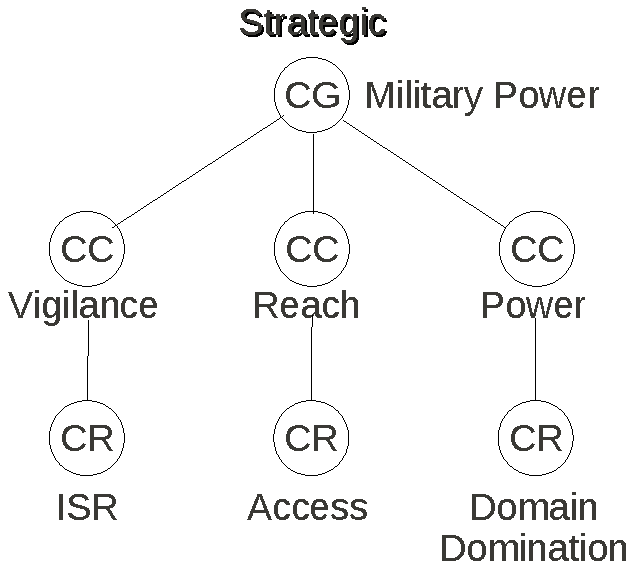
\includegraphics[width=0.6\linewidth]{Figures/milPowerCOG}}
    \end{minipage}
    &
    \begin{minipage}{0.48\linewidth}
     \centering{ 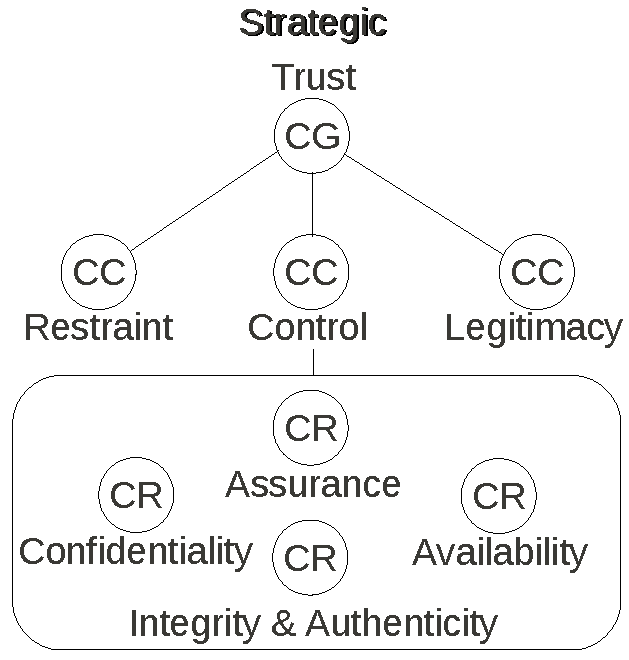
\includegraphics[width=0.6\linewidth]{Figures/trustCOG}}\\
   \end{minipage}\\
   (a) Military Power as a Center of Gravity & (b) Trust as a Center of Gravity\\
  \end{tabular}
  \caption{Military Power and Trust Centers of Gravity}
  \label{fig:cogs}
\end{figure}

Centers of gravity (CGs) are the \emph{primary sources of moral or
  physical strength, power and resistance}.  CGs are \emph{hubs of all
  power}.  In war, a strategic objective is to destroy or neutralize
an adversary's centers of gravity.  By so doing, the adversary is
\emph{dislocated}, i.e., thrown off balance, so that their ability to
operate quickly, decisively, precisely, and correctly is degraded.

Centers of gravity emerge from a collection of primary abilities known
as \textbf{critical capabilities} in the context of a given mission or
scenario.  For example, the combined capabilities of ground, air, and
space surveillance contribute the the critical capability of
\emph{global vigilance} that is one of three critical capabilities
(the others being global reach and global power) that are the basis
for US military as a center of gravity---a hub of US power.

Another center of gravity is \textbf{trust}. Trust and trustworthiness
are crucial at all levels of war and at all levels in
cyberspace. Trust and trustworthiness are both the glue that holds
systems together as well as the oil that keeps systems running
smoothly.  Without trust, systems freeze. In the 2008 financial crisis
that threatened to bankrupt several US banks and financial services
companies, a root cause for the near total disintegration of the
global economy was the fact that loans, risk assessments, property
values, and hence the balance sheets of banks were untrustworthy. When
the lack of trustworthiness of information became apparent, trust
evaporated and the global financial system disintegrated and froze.

In military systems, there are three critical capabilities that
constitute trust as a center of gravity.
\begin{enumerate}
\item Restraint: the ability to exercise appropriate self-control, in
  this case the ability to react with appropriate proportionality,
\item Legitimacy: the acceptance of our actions because of the
  appropriateness of the actions given a particular circumstance,
\item Control: the ability to command and control our forces and
  systems with complete integrity, accuracy, and accountability.
\end{enumerate}
Figure~\ref{fig:cogs}(a) shows military power as a center of gravity
and its critical capabilities and requirements. In an environment
heavily dependent on computer-enabled communications, command and
control, and intelligence (C3I), the trustworthiness of the
computational infrastructure in terms of hardware, software, networks,
and protocols is essential, as is the trustworthiness of the
access control employed from control of physical memory up to and
including information flow policies. Thus, \textbf{trust} as a
strategic center of gravity is alongside military power as a CG.

\paragraph{Assurance of Integrity and Authenticity}

Figure~\ref{fig:cogs}(b) shows trust as a center of gravity along with
the critical capability of \emph{control}. Positive control of forces
requires assurance of confidentiality, availability, and integrity and
authenticity. Again, imagine if operators could not believe the
information or the orders they received. They would be dislocated and
paralyzed. Given the criticality of integrity and authenticity, it is
essential that the highest degree of precision and accuracy of
understanding combined with the highest degree of assurance of
integrity and authenticity be provided to critical missions.  The use
of the access-control logic combined with formal verifications in HOL
enable a rapid, precise, and accurate assessment of the integrity and
authentication CONOPS. As everything is fully disclosed and nothing is
left to the imagination, rapid, precise, and accurate \emph{conceptual
  unity} is achieved.

\section{Assumptions}
\label{sec:assumptions}

Your solutions will be crafted to work in an existing trust
infrastructure that includes:
\begin{enumerate}
\item a hierarchy of certificate authorities to authenticate
  cryptographic keys, provide attribution for messages, and
  authenticate mission roles;
\item the root of trust for cryptographic keys, i.e., the public key
  for the Joint Forces Certificate Authority, $K_{JFCA}$ will be
  distributed in a secure manner to commanders, operators, and weapons
  prior to the mission start;
\item established mission roles in terms of what commands each role
  controls;
\item formally defined mission commands and weapon commands.
\end{enumerate}

\paragraph{Certificate Authority Hierarchy}
\begin{figure}[t]
  \centering
  \begin{tabular}[t]{cc}
    \begin{minipage}{0.48\linewidth}
      % \begin{figure}[t]
      \centering
      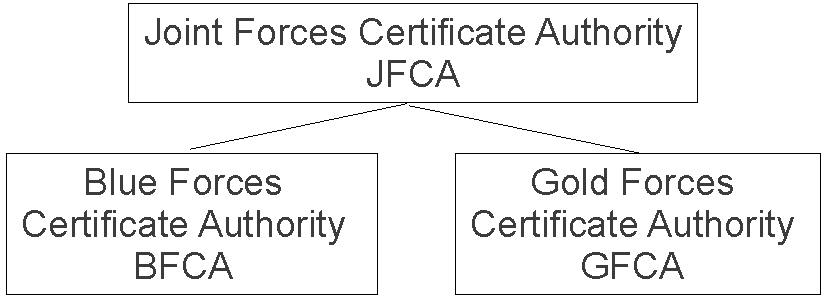
\includegraphics[width=0.95\linewidth]{Figures/CAHierarchy}
      % \caption{Certificate Authority Hierarchy}
      % \label{fig:ca-hierarchy}
      % \end{figure}
    \end{minipage}
    &
    \begin{minipage}{0.48\linewidth}
      % \begin{figure}[t]
      \centering
      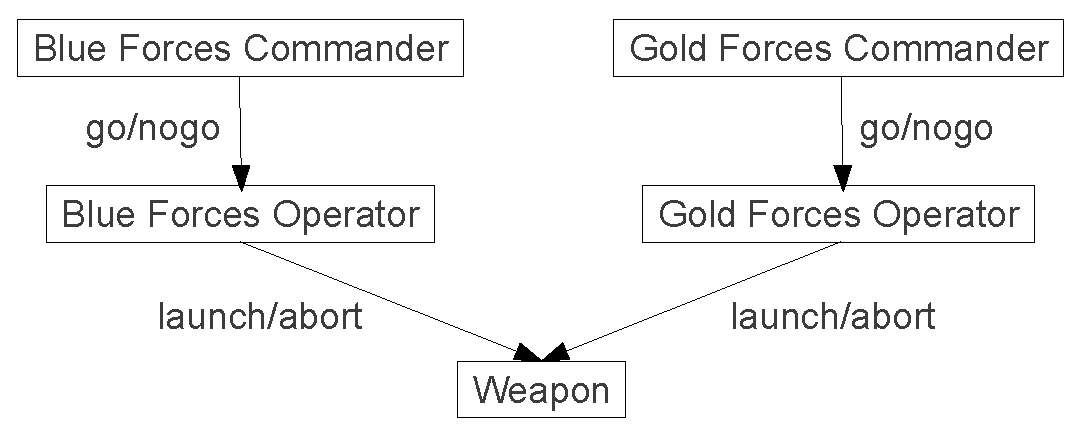
\includegraphics[width=0.95\linewidth]{Figures/conops}
      % \caption{Flow of Command and Control}
      % \label{fig:c2-flow}
      % \end{figure}
    \end{minipage}\\
    (a) Certificate Authority Hierarchy & (b) Flow of Command and Control\\
  \end{tabular}
  
  \caption{Certificate Authority Hierarchy and Flow of Command and Control}
\label{fig:ca-hierarchy-c2-flow}
\end{figure}





Figure~\ref{fig:ca-hierarchy-c2-flow}(a) shows the relationships among the Joint
Forces Certificate Authority (JFCA), Blue Forces Certificate Authority
(BFCA), and Gold Forces Certificate Authority (GFCA).  The primary
purpose of the JFCA is to authenticate the BFCA and GFCA for specific
missions.  Note, it could very well be the case that each joint forces
mission has a different JFCA.  This prevents ``mission creep'' in
terms of authorizations for one mission leaking over to separate
missions.

The BFCA and GFCA are anticipated to be the CAs normally recognized by
Blue and Gold Forces, respectively.  There is no need for cross
recognition of BFCAs or GFCAs independently of the JFCA.  This is
consistent with the intent of establishing JFCAs on a
mission-by-mission basis.

We have the following structure:

\begin{center}
  \begin{tabular}[h]{|r| >{$}c<{$}|l|}
    \hline
    \textbf{Certificate Authority} &\textbf{Associated Key} & \textbf{How Authenticated}\\
    \hline
    JFCA & K_{JFCA} & Pre-distributed to all mission principals\\
    Blue Forces CA & K_{BFCA} & Authenticated by JFCA\\
    Gold Forces CA & K_{GFCA} & Authenticated by JFCA\\
    \hline
  \end{tabular}
\end{center}



\paragraph{Mission Roles and Jurisdiction}

The following mission roles and their authority are stated below.

\begin{center}
  \begin{tabular}[h]{|r| >{$}c<{$}|l|}
    \hline
    \textbf{Role} & \textbf{Controls} & \textbf{How Authenticated}\\
    \hline
    Blue Forces Commander & \texttt{go}/\texttt{nogo} & Pre-distributed to all Blue Forces mission principals\\
    Gold Forces Commander & \texttt{go}/\texttt{nogo} & Pre-distributed to all Gold Forces mission principals\\
    Blue Forces Operator & \texttt{launch}/\texttt{abort} & Blue Forces Commander\\
    Gold Forces Commander & \texttt{launch}/\texttt{abort} & Gold Forces Commander\\
    \hline
  \end{tabular}
\end{center}

\paragraph{Mission Commands and Weapon Commands}
The mission is initiated with a \texttt{go} command; it is aborted
with a \texttt{nogo} command. Mission commands are defined as follows.
\begin{gather*}
  missionCommands \isa go \ora nogo.
\end{gather*}
Weapon commands are defined as follows.
\begin{gather*}
  weaponCommands \isa launch \ora abort.
\end{gather*}
The flow of command and control is shown in Figure~\ref{fig:ca-hierarchy-c2-flow}.

\paragraph{Weapons Policy}

The weapons policy is as follows.
\begin{center}
  \begin{tabular}[h]{|r|l|}
    \hline
    \textbf{Action} & \textbf{Command and Control Requirements}\\
    \hline
    Weapons Launch & \emph{Launch} ordered by both Blue and Gold Operators\\
    Weapons Abort & \emph{Abort} ordered by either Blue or Gold Operator\\
    \hline
  \end{tabular}
\end{center}

% Full technical details for each of the above elements is fully
% disclosed as HOL theories in Section~\ref{sec:techniques-tools}.

\section{Rigorous Representations of Concept of Operations}


\begin{figure}[t]
  \centering
  \begin{tabular}{cc}
    \begin{minipage}{0.48\linewidth}
      \centering{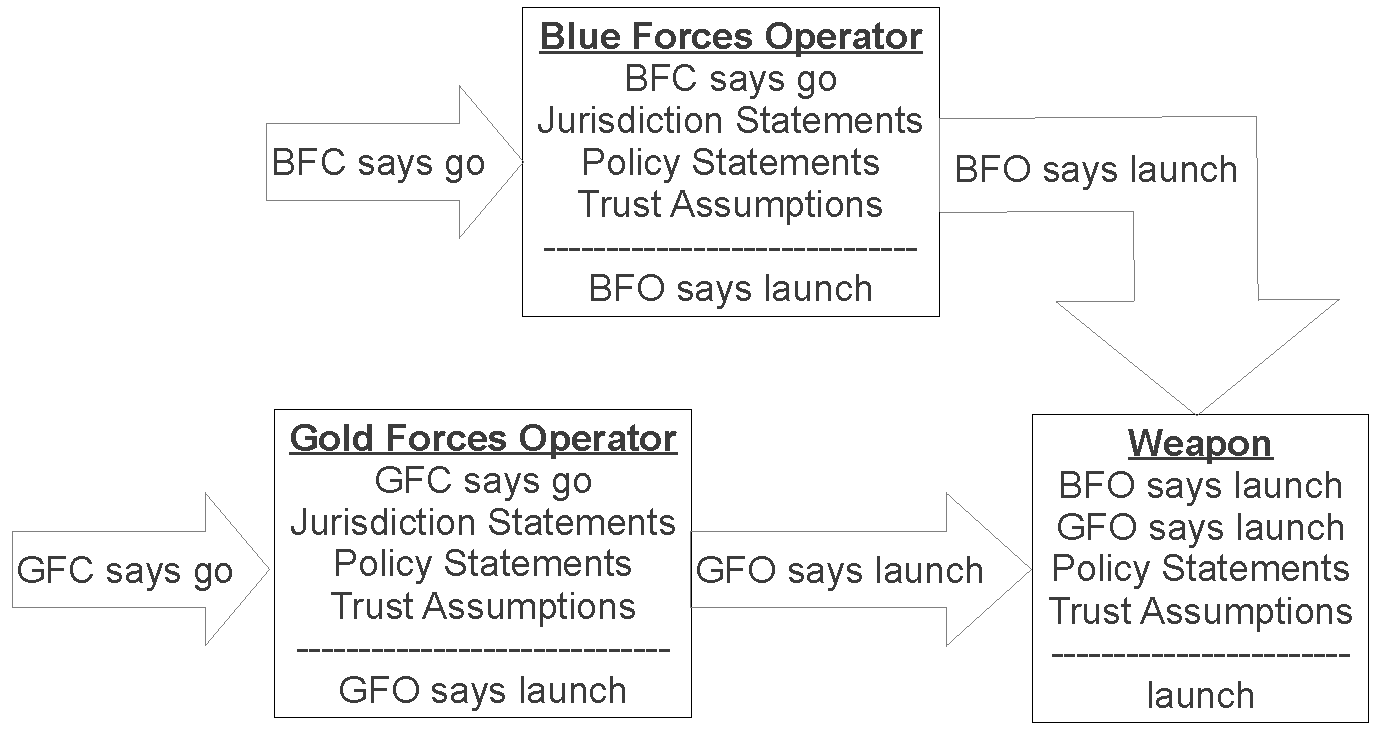
\includegraphics[width=0.95\linewidth]{Figures/launchCONOPS}}
    \end{minipage}
    &
    \begin{minipage}{0.48\linewidth}
      \centering{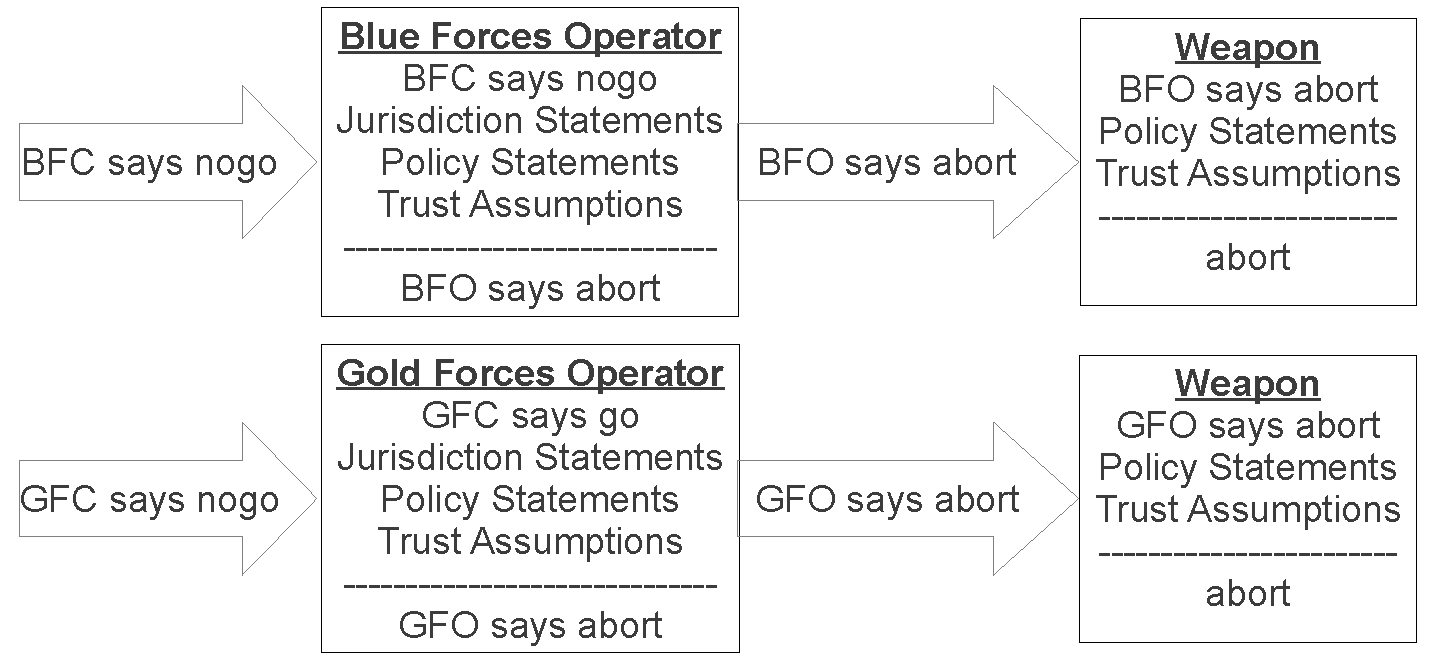
\includegraphics[width=0.95\linewidth]{Figures/abortCONOPS}}
    \end{minipage}\\
    (a) Launch CONOPS & (b) Abort CONOPS\\
  \end{tabular}
  \caption{High-Level View of Launch and Abort CONOPS}
  \label{fig:launch-abort-conops}
\end{figure}

\begin{table}[t]
  \centering
  \begin{tabular}{cc}
  \begin{minipage}{0.4\linewidth}
    \begin{center}
      \begin{tabular}{|r<{.}>{$}l<{$}l|}
        \hline
        1 & P \says \varphi_1 & Received command\\
        2 & P \controls \varphi_1 & Jurisdiction of P\\
        3 & \varphi_1 \implies \varphi_2 & Policy assumption\\
        4 & \varphi_1 & 2, 1 Controls\\
        5 & \varphi_2 & 4, 3 Modus Ponens\\
        6 & Q \says \varphi_2 & 5 Says\\
        \hline
      \end{tabular}
    \end{center}
  \end{minipage}
  &
  \begin{minipage}{0.6\linewidth}
    \begin{center}
      \begin{tabular}{|r<{.}>{$}p{0.45\linewidth}<{$}l|}
        \hline
        1 & P \says \varphi & Received command\\
        2 & Q \says \varphi & Received command\\
        3 & P \with Q \controls \varphi & Dual control policy\\
        4 & (P \says \varphi) \wedge (Q \says \varphi) & 1, 2 Conjunction\\
        5 & (P \says \varphi) \wedge (Q \says \varphi) \equiv P \with Q \says \varphi & \& Says\\
        6 & P \with Q \says \varphi & 5, 4 Equivalence\\
        7 & \varphi & 6, 3 Controls\\
        \hline
      \end{tabular}
    \end{center}

  \end{minipage}\\
  (a) Proof of Implied Controls with Says& (b) Proof of Dual Control
\end{tabular}
  \caption{Proof of Implied Controls with Says Inference Rule}
  \label{tab:implied-controls-with-says-proof}
\end{table}

\begin{table}[t]
  \centering
  \begin{tabular}{cc}
  \begin{minipage}{0.48\linewidth}
    \begin{center}
      \begin{tabular}{|r<{.}>{$}p{0.45\linewidth}<{$}l|}
        \hline
        1 & P \says \varphi & assumption\\
        2 & P \controls \varphi \wedge Q \controls \varphi & assumption\\
        3 & P \controls \varphi & 2 Simplification (1)\\
        4 & \varphi & 2, 1 Controls\\
        \hline
      \end{tabular}
    \end{center}
  \end{minipage}
    &
    \begin{minipage}{0.48\linewidth}
      \begin{center}
        \begin{tabular}{|r<{.}>{$}p{0.45\linewidth}<{$}l|}
          \hline
          1 & Q \says \varphi & assumption\\
          2 & P \controls \varphi \wedge Q \controls \varphi & assumption\\
          3 & Q \controls \varphi & 2 Simplification (2)\\
          4 & \varphi & 2, 1 Controls\\
          \hline
        \end{tabular}
      \end{center}
  \end{minipage}\\
  (a) Proof of Alternate Controls (1) & (b) Proof of Alternate Controls (2)
\end{tabular}
  \caption{Proof of Alternate Controls Rule}
  \label{tab:alternate-controls-proof}
\end{table}

% \subsection{Representing Concepts of Operations in the Access-Control
%   Logic}
% \label{sec:conops}

\begin{center}
  \fbox{\begin{minipage}[h]{0.8\linewidth} Definition of
      \textbf{Concept of Operations}: JP 5-0, Joint Operation Planning
      \begin{small}
        \begin{quote}
          \emph{ ``The CONOPS clearly and concisely expresses what [is
            to be] accomplish[ed] and how it will be done using
            available resources. It describes how the actions of
            $\ldots$ components and supporting organizations will be
            integrated, synchronized, and phased to accomplish the
            mission $\ldots$''}
        \end{quote}
      \end{small}
    \end{minipage}}
\end{center}

Concepts of operations (CONOPS) as stated in the JP 5-0, Joint
Operation Planning definition, describes the coordination,
integration, and sequencing of actions of components and
organizations.  From a command and control standpoint, we focus on the
flow of commands from one principal to the next (recalling that
principals are people, roles, cryptographic keys, processes, etc.),
within a context of policies that govern actions, jurisdiction of
controlling authorities, and trust assumptions.  Using the
access-control logic, each step in a CONOPS---\textbf{a response by a
  principal corresponding to a component in the CONOPS} to a command,
request, or statement in conjunction with policies, jurisdiction of
controlling authorities, and trust assumptions---is a derived
inference rule in the logic. 

Each rule serves as a logical justification of the actions of a CONOPS
component to specific situations. The advantages of using formally
proved inference rules include: (1) establishing the operating
assumptions on which logical validity is based, (2) assurance and full
disclosure due to formal verification, and (3) conceptual unity, when
descriptions and verifications are done and distributed using
computer-assisted reasoning tools such as HOL.

In the three sections that follow, we give three views of the CONOPS
created to satisfy the flow of command and control and certificate
authority hierarchy shown in
Figure~\ref{fig:ca-hierarchy-c2-flow}. Section~\ref{sec:high-level-conops}
gives a high-level description of CONOPS using only the mission roles
of Blue Forces Commander, Blue Forces Operator, Gold Forces Commander,
Gold Forces Operator, and the
Weapon. Section~\ref{sec:conops-with-staff} refines the high-level
CONOPS description by adding people assigned to mission
roles. Section~\ref{sec:conops-with-keys} is the final refinement that
adds cryptographic keys to the flow of control along with certificate
authority hierarchy in Figure~\ref{fig:ca-hierarchy-c2-flow}(a).

\subsection{High-Level CONOPS Description Using Only Mission Roles}
\label{sec:high-level-conops}

Figure~\ref{fig:launch-abort-conops}(a) and (b) show the high-level
CONOPS for launching or aborting the weapon, respectively. Each box
represents a \emph{derived inference rule} in the access-control
logic. The view is high level because the rules are expressed in terms
of roles only.

Notice that the form of Figures~\ref{fig:launch-abort-conops}(a) and
\ref{fig:launch-abort-conops}(b) correspond to the flow of command and
control as shown in Figure~\ref{fig:ca-hierarchy-c2-flow}(b). The
difference is that Figure~\ref{fig:launch-abort-conops} makes all the
hypotheses and conclusions explicit in the form of derived inference
rules. For example, take the box corresponding to \emph{Blue Forces
  Operator}.  \emph{BFO} receives an order from the Blue Forces
Commander: $BFC \says \action{go}$. The Blue Forces Operator evaluates
$BFC \says \action{go}$ in the context of jurisdiction statements,
policy statements, and trust assumptions.  If the Blue Forces Operator
concludes \action{Launch}, then (using the \emph{Says} rule), the Blue
Forces Operator issues the \emph{Launch} command, i.e., $BFO \says
\action{Launch}$.

Essentially, what we must do based on the informal CONOPS statements
and assumptions is write the jurisdiction statements, policy
statements, and trust assumptions necessary for the Blue Forces
Operator to conclude \emph{Launch} when he/she receives the \emph{go}
command from the Blue Forces Commander. 

Perhaps the most straightforward derived inference rule for the Blue
Forces Operator is:
\begin{gather*}
  \irule
  {
    \begin{array}{c}
      BFC \says \action{go} \quad BFC \controls \action{go}\quad
      \action{go} \implies \action{launch}\\
    \end{array}
  }
  {BFO \says \action{launch}}
  {BFO Launch}
\end{gather*}
If the derived inference rule for the Gold Forces Operator has exactly
the same form, i.e.,
\begin{gather*}
  \irule
  {
    \begin{array}{c}
      GFC \says \action{go} \quad GFC \controls \action{go}\quad
      \action{go} \implies \action{launch}\\
    \end{array}
  }
  {GFO \says \action{launch}}
  {GFO Launch},
\end{gather*}
then both Blue and Gold Operators are relying a general inference rule:
\begin{gather*}
  \irule
  {
    \begin{array}{c}
      P \says \varphi_1 \quad P \controls \varphi_1\quad
      \varphi_1 \implies \varphi_2\\
    \end{array}
  }
  {Q \says \varphi_2}
  {Implied Controls with Says}.
\end{gather*}
The proof of the \emph{Implied Controls with Says} inference rule is
shown in Table~\ref{tab:implied-controls-with-says-proof}.
Discovering common logical principles and rules is an advantage
intrinsic to using symbolic logic in general, as well as the
access-control logic in particular.

Turning to the derived inference rule corresponding to the weapon, we
have the following inference rule:
\begin{gather*}
  \irule
  {
    \begin{array}[h]{c}
      P \says \varphi \quad Q \says \varphi \quad P \with Q \controls \varphi
    \end{array}
  }
  {\varphi}
  {Dual Control}
\end{gather*}
The proof of \emph{Dual Control} is given in
Table~\ref{tab:implied-controls-with-says-proof}(b).

Finally, we turn to the high-level abort CONOPS, as shown in
Figure~\ref{fig:launch-abort-conops}(b). Both the Blue and Gold
Operators can have the same abort policy:
\begin{gather*}
  \irule
  {
    \begin{array}{c}
      BFC \says \action{nogo} \quad BFC \controls \action{nogo} \quad
      \action{nogo} \implies \action{abort}
    \end{array}
  }
  {BFO \says \action{abort}}
  {BFO Abort}\\
  \irule
  {
    \begin{array}{c}
      GFC \says \action{nogo} \quad GFC \controls \action{nogo} \quad
      \action{nogo} \implies \action{abort}
    \end{array}
  }
  {GFO \says \action{abort}}
  {GFO Abort}
\end{gather*}
Both are instances of the \emph{Implied Controls with Says} rule. 

The weapons \emph{abort} rules are as follows:
\begin{gather*}
  \irule
  {
    \begin{array}{c}
      BFO \says \action{abort} \quad BFO \controls \action{abort} \wedge
      GFO \controls \action{abort}
    \end{array}
  }
  {\action{abort}}
  {BFO Weapons Abort}\\
  \irule
  {
    \begin{array}{c}
      GFO \says \action{abort} \quad BFO \controls \action{abort} \wedge
      GFO \controls \action{abort}
    \end{array}
  }
  {\action{abort}}
  {GFO Weapons Abort}.
\end{gather*}
Both are instances of two similar rules, proved in
Table~\ref{tab:alternate-controls-proof}(a) and
Table~\ref{tab:alternate-controls-proof}(b). The rules are shown
below.
\begin{gather*}
  \irule
  {
    \begin{array}{c}
      P \says \varphi \quad P \controls \varphi \wedge
      Q \controls \varphi
    \end{array}
  }
  {\varphi}
  {Alternate Controls (1)}\\
  \irule
  {
    \begin{array}{c}
      Q \says \varphi \quad P \controls \varphi \wedge
      P \controls \varphi
    \end{array}
  }
  {\varphi}
  {Alternate Controls (2)}.  
\end{gather*}

\subsection{Refined CONOPS with Principals Authenticated into Mission Roles}
\label{sec:conops-with-staff}

\begin{figure}[t]
  \centering
  \begin{tabular}{cc}
    \begin{minipage}{0.48\linewidth}
      \centering{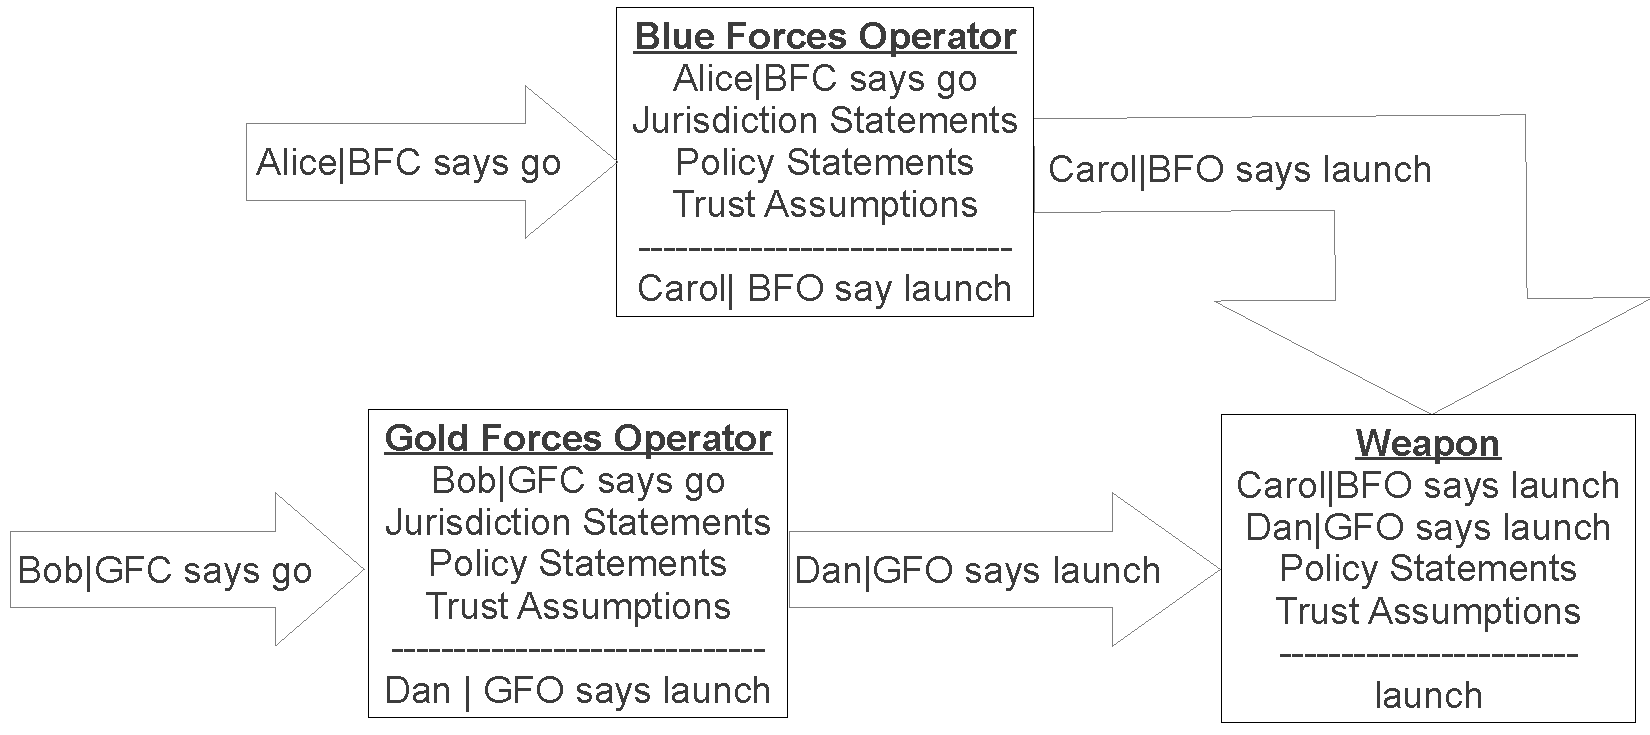
\includegraphics[width=0.95\linewidth]{Figures/launchCONOPSRefine1}}
    \end{minipage}
    &
    \begin{minipage}{0.48\linewidth}
      \centering{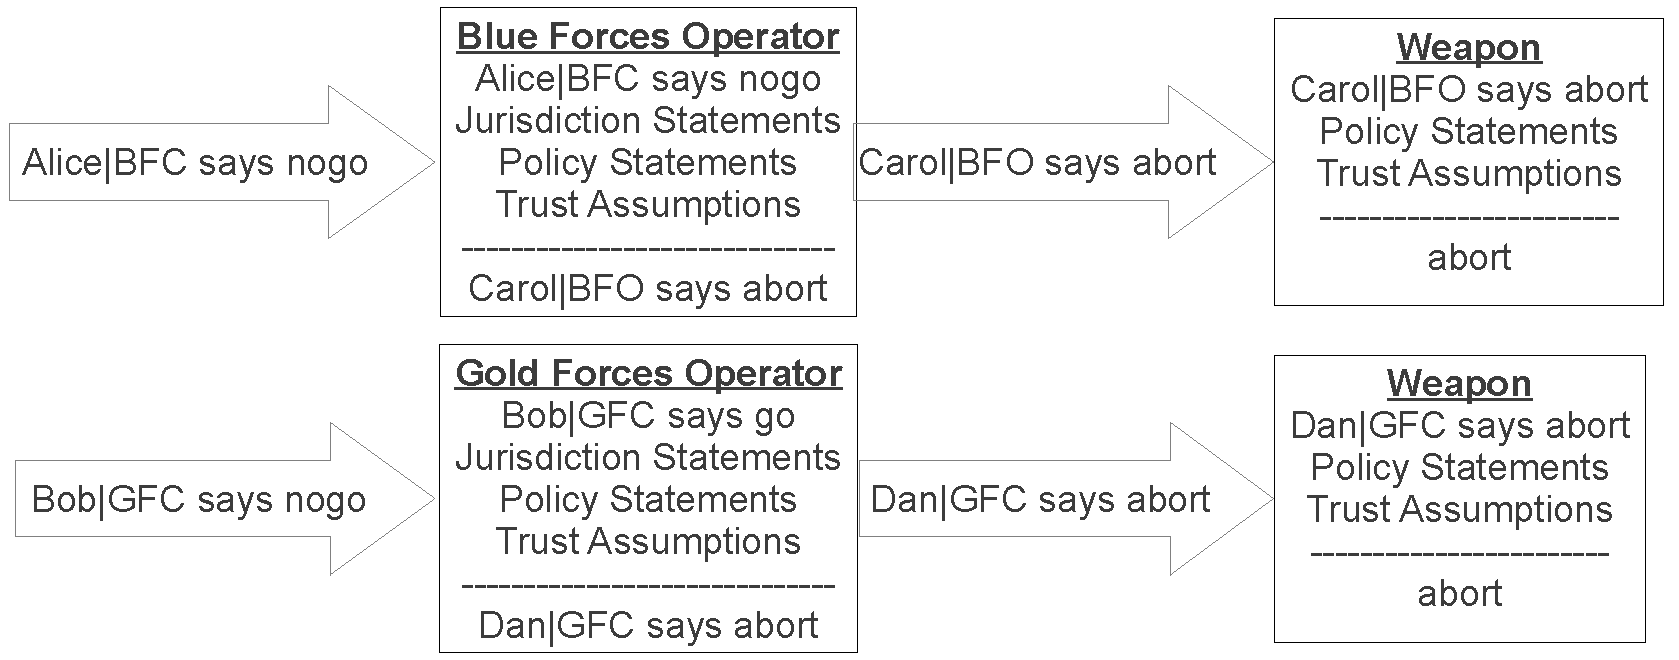
\includegraphics[width=0.95\linewidth]{Figures/abortCONOPSRefine1}}
    \end{minipage}\\
    (a) Launch CONOPS & (b) Abort CONOPS\\
  \end{tabular}
  
  \caption{Launch and Abort CONOPS with Assigned Personnel}
  \label{fig:conops-with-people}
\end{figure}

\begin{table}[t]
  \centering
  \begin{tabular}{|c|c|>{$}l<{$}|}
    \hline
    \textbf{Role} & \textbf{Description of Authority} & 
    \textbf{Formal Description of Authority}\\
    \hline
    Blue Forces Commander (BFC) & go & BFC \controls \action{go}\\
    & nogo & BFC \controls \action{nogo}\\
    & Assignment of BF Operators & BFC \controls (\reps{P}{BFO}{\varphi})\\
    \hline
    Gold Forces Commander (GFC) & go & GFC \controls \action{go}\\
    & nogo & GFC \controls \action{nogo}\\
    & Assignment of GF Operators & GFC \controls (\reps{P}{GFO}{\varphi})\\
    \hline
    Blue Forces Operator (BFO) & launch & BFO \controls \action{launch}\\
    & abort & BFO \controls \action{abort}\\
    \hline
    Gold Forces Operator (GFO) & launch & GFO \controls \action{launch}\\
    & abort & GFO \controls \action{abort}\\
    \hline
  \end{tabular}
  \caption{Mission Roles and Their Authority}
  \label{tab:roles-authority}
\end{table}
\begin{table}[t]
  \centering
  \begin{center}
  \begin{tabular}[h]{|r|l|l|>{$}p{0.43\linewidth}<{$}|}
    \hline
    \textbf{Role} & \textbf{Person} & \textbf{Authenticated By} & \textbf{Formal Description of Delegation of Authority}\\
    \hline
    BFC & Alice & pre-distributed prior to mission & 
    \reps{Alice}{BFC}{\varphi} \\
    & & & \reps{Alice}{BFC}{(\reps{Carol}{BFO}{\varphi})}\\
    GFC & Bob & pre-distributed prior to mission & 
    \reps{Bob}{GFC}{\varphi}\\
    & & & \reps{Bob}{GFC}{(\reps{Dan}{GFO}{\varphi})}\\
    BFO & Carol & Alice as BFC & \reps{Carol}{BFO}{\varphi}\\
    GFO & Dan & Bob as GFC & \reps{Dan}{GFO}{\varphi}\\
    \hline
  \end{tabular}
\end{center}
\caption{Role Assignments and Authorizations}
\label{tab:role-assignments}
\end{table}

The first refinement to the high-level CONOPS expressed only in terms
of mission roles is to add the notion of authentication of principals
acting in mission roles. A principal $P$ acting in a mission role
\emph{Role} giving command $\varphi$ is represented by $P \quoting
Role \says \varphi$. If \emph{P's} authority to act in role
\emph{Role} is recognized, i.e., $\reps{P}{Role}{\varphi}$, and if
$Role \controls \varphi$, then we conclude $\varphi$ is justified,
from the \emph{Reps} inference rule shown below:
\begin{gather*}
  \irule
  {Q \controls \varphi \quad \reps{P}{Q}{\varphi} \quad 
   P \quoting Q \says \varphi}
  {\varphi}
  {Reps}.
\end{gather*}
Figure~\ref{fig:conops-with-people} is a block diagram that refines
the high-level launch and abort CONOPS in
Figure~\ref{fig:launch-abort-conops}.  The primary differences are in
the messages sent among principals. Instead of mission roles speaking,
principals claiming to be acting in mission roles make
statements. Figure~\ref{fig:conops-with-people} shows Alice acting as
Blue Forces Commander, Bob acting as Gold Forces Commander, Carol
acting as Blue Forces Operator, and Dan acting as Gold Forces
Operator.

From the assumptions in Section~\ref{sec:assumptions}, we recall that
Blue and Gold Forces Commanders have the authority to assign personnel
to the roles of Blue and Gold Operators, respectively:
\begin{gather*}
  BFC \controls (\reps{P}{BFO}{\varphi})\\
  GFC \controls (\reps{P}{GFO}{\varphi}).
\end{gather*}
Table~\ref{tab:roles-authority} gives a complete listing of roles and
their associated authority. Table~\ref{tab:role-assignments} shows the
personnel assignments to mission roles and who authenticates them.
Notice that authorizations for personnel designated as Blue and Gold
Forces Commanders are designated as \emph{pre-distributed prior to
  mission}. This is similar to the case where the cryptographic key of
a root certificate authority is pre-loaded into computers. In this
CONOPS, mission equipment and weapons must be loaded with
\textbf{roots of trust} prior to the start of the mission. In this
case, it will include the personnel who are authorized as commanders
as well as cryptographic keys of root authorities. \textbf{The loading
  of this information must be done with the utmost integrity and
  security otherwise all is lost.}

\paragraph{Derived Inference Rules}
\label{sec:deriv-infer-rules}

We now refine the derived inference rules corresponding to BFO Launch,
GFO Launch, BFO Abort, GFO Abort, and when the weapon is launched or
aborted.

\subparagraph{BFO and GFO Launch}
\label{sec:bfo-gfo-launch}

\begin{table}[t]
  \centering
  \begin{tabular}{|r<{.}>{$}l<{$}l|}
    \hline
    1 & Q \controls \varphi_1 & Assumption, jurisdiction of Q\\
    2 & \reps{P}{Q}{\varphi} & P acting in role of Q\\
    3 & P \quoting Q \says \varphi_1 & Command from P\\
    4 & \varphi_1 \implies \varphi_2 & Policy statement\\
    5 & \varphi_1 & 1, 2, 3 Reps\\
    6 & \varphi_2 & 5, 4 Modus Ponens\\
    7 & R \says \varphi_2 & 6 Says\\
    \hline
  \end{tabular}
  \caption{Proof of Implied Controls with Delegation}
  \label{tab:delegation-proof}
\end{table}
Based on Figure~\ref{fig:conops-with-people} we refine the derived
inference rules \emph{BFO Launch} and \emph{GFO Launch} based on the
form of received orders and the trust assumptions and policy
statements needed by operators to issue the launch command to the
weapon.

As we are using delegation of principals to mission roles as a means
for assigning people to mission roles, our launch rules for operators
require operators to know who is operating in the role of Blue or Gold
Forces Commander. This knowledge is reflected in the statements
$\reps{Alice}{BFC}{\action{go}}$ and $\reps{Bob}{GFC}{\action{go}}$.
\begin{gather*}
  \irule
  {
    \begin{array}{c}
      BFC \controls \action{go} \quad \reps{Alice}{BFC}{\action{go}} \quad 
      Alice \quoting BFC \says \action{go} \quad \action{go} \implies \action{launch}
    \end{array}
  }
  {Carol \quoting BFO \says \action{launch}}
  {BFO Launch} \\
  \irule
  {
    \begin{array}{c}
      GFC \controls \action{go} \quad \reps{Bob}{GFC}{\action{go}} \quad 
      Bob \quoting GFC \says \action{go} \quad \action{go} \implies \action{launch}
    \end{array}
  }
  {Dan \quoting GFO \says \action{launch}}
  {GFO Launch}
\end{gather*}
We see that as before both of the Launch rules are instances of the
same rule:
\begin{gather*}
  \irule
  {\begin{array}{c}
      Q \controls \varphi_1 \quad \reps{P}{Q}{\varphi_1} \quad 
      P \quoting Q \says \varphi_1 \quad \varphi_1 \implies \varphi_2
    \end{array}
  }
  {R \says \varphi_2}
  {Implied Controls with Delegation}
\end{gather*}

% \subparagraph{BFO and GFO Abort}
% \label{sec:bfo-gfo-abort}

\begin{center}
  \problembox{
    \begin{enumerate}
    \item Add another LaTeX subparagraph titled \textbf{BFO and GFO
        Abort} that details as \emph{proved inference rules}:
      \begin{enumerate}[{a.}]
      \item when Blue and Gold Forces Operators issue abort commands,
        and
      \item the conditions under which the Weapon will abort.
      \end{enumerate}
    \item Your inference rules should be presented in the style of the
      other inference rules in this section.
    \item Your proofs should be presented in the style of the proofs
      shown in the tables in this section.
    \end{enumerate}

    % A similar set of refinements can be worked out for aborting the
    % mission and the weapon. \textbf{\redtext{Your problem solution
    % will include the refinements for aborting the mission.}}
  }
\end{center}
\subsection{Refined CONOPS Using Cryptographic Keys}
\label{sec:conops-with-keys}

\begin{figure}[t]
  \centering
  \begin{tabular}{cc}
    \begin{minipage}{0.48\linewidth}
      \centering{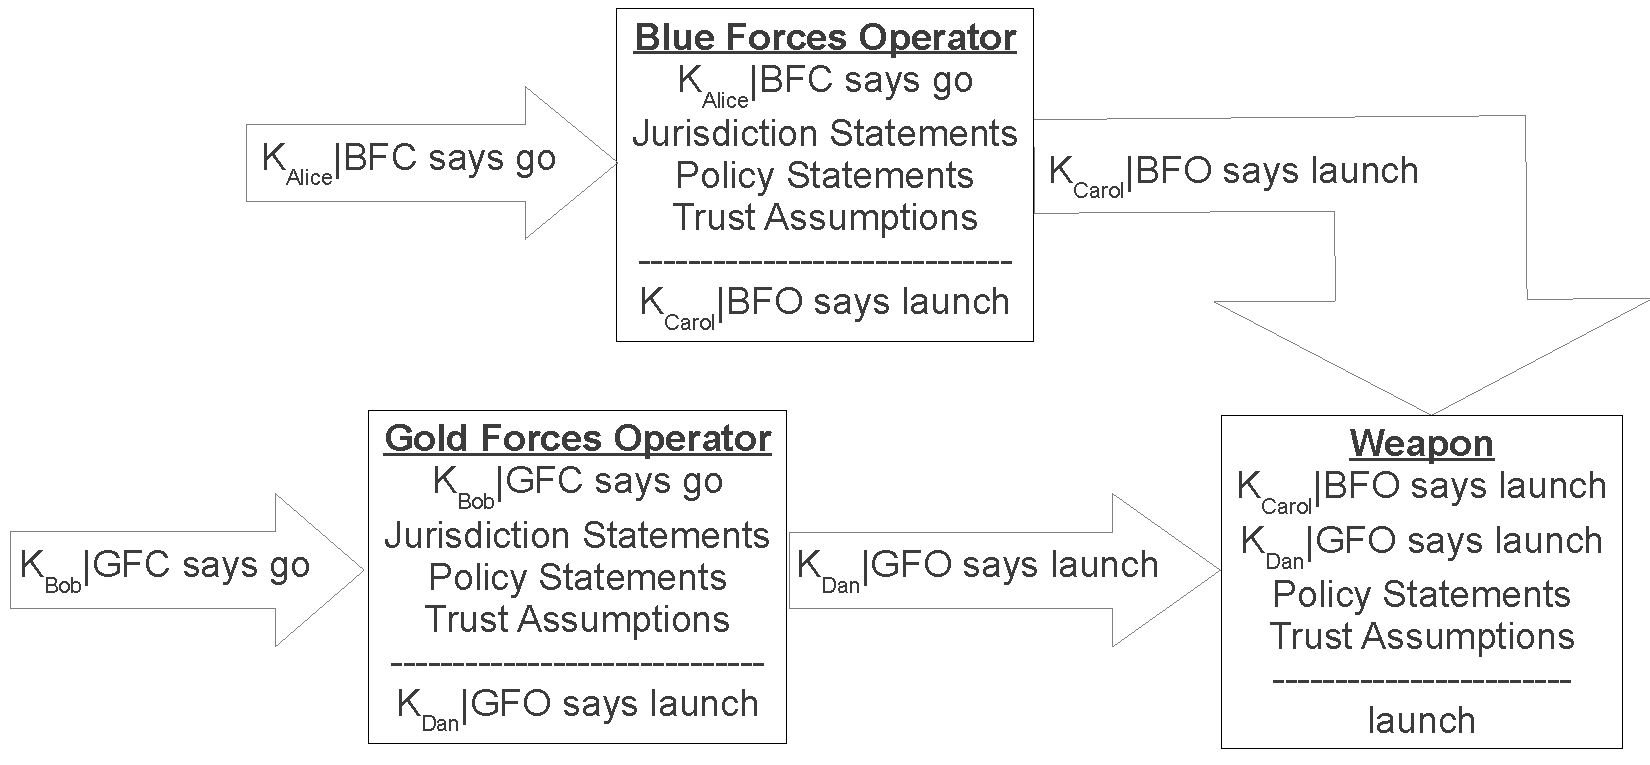
\includegraphics[width=0.95\linewidth]{Figures/launchCONOPSRefine2}}
    \end{minipage}
    &
    \begin{minipage}{0.48\linewidth}
      \centering{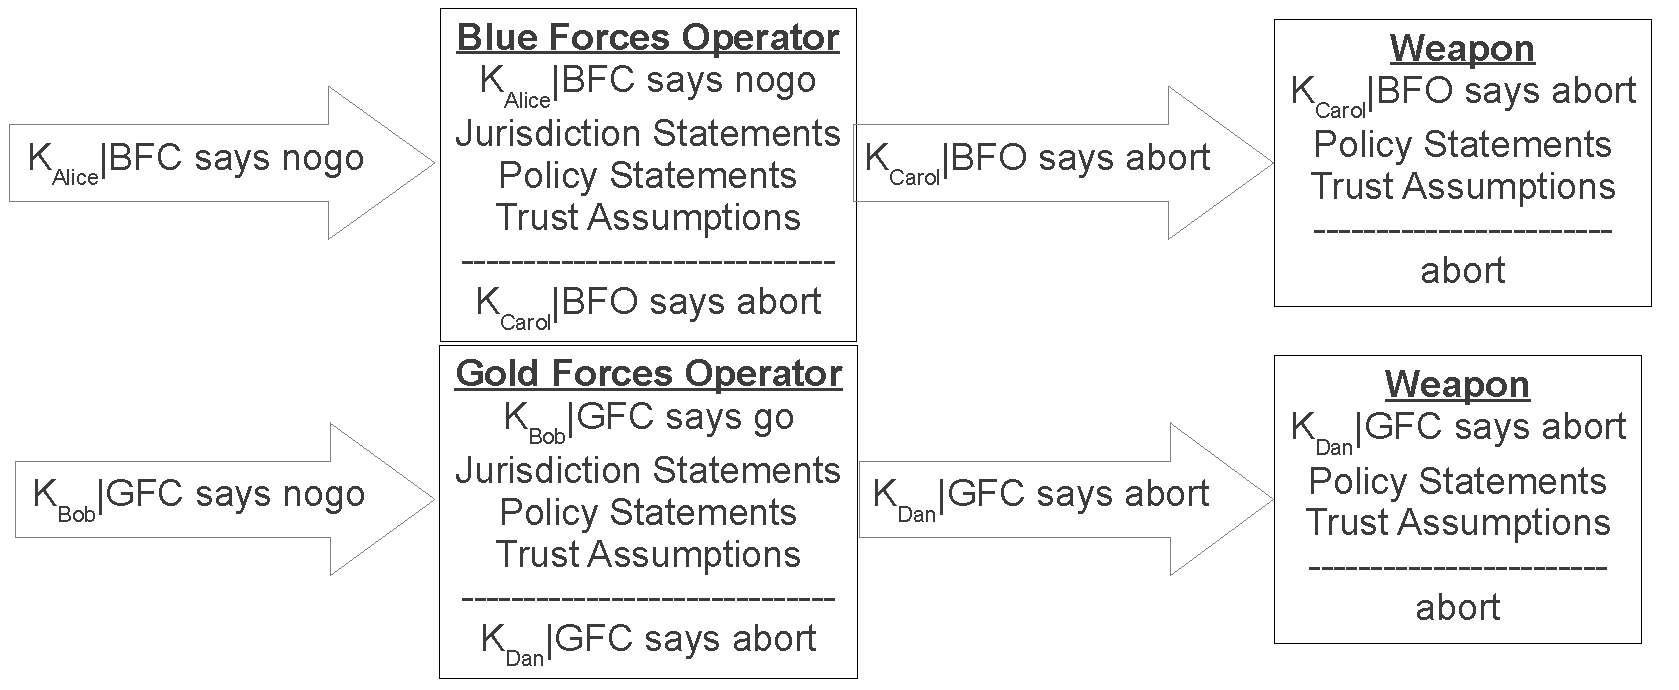
\includegraphics[width=0.95\linewidth]{Figures/abortCONOPSRefine2}}
    \end{minipage}\\
    (a) Launch CONOPS & (b) Abort CONOPS\\
  \end{tabular}
  
  \caption{Launch and Abort CONOPS with Cryptographic Keys}
  \label{fig:launch-abort-conops-crypto}
\end{figure}

\begin{center}
  \problembox{Figure~\ref{fig:launch-abort-conops-crypto} is a CONOPS
    that refines the CONOPS in Figure~\ref{fig:conops-with-people} by
    adding the use of cryptographic keys for identification. Your
    problem solution will:
    \begin{enumerate}
    \item Detail the use of cryptographic keys for authenticating the
      integrity of command and control in this CONOPS.
    \item Your solution
      will work within the certificate hierarchy, flow of command and
      control, and jurisdiction of roles described in the assumptions
      in Section~\ref{sec:assumptions}.
    \item As in the high-level and
      refined CONOPS, your solution will show the logical
      justification for each step in the CONOPS in the form of a
      formally proved derived inference rule.
    \item Your inference rules should be presented in the style of the
      other inference rules in the previous sections.
    \item Your proofs should be presented in the style of the proofs
      shown in the tables in the previous sections.
    \end{enumerate}
}
\end{center}


\section{Formal Description and Verification of CONOPS in HOL}

In this section we give the HOL theories used to describe the CONOPS
at three levels of detail. In Section~\ref{sec:mission-roles-conops}
are the HOL theories used to describe and verify the top-level CONOPS
using only mission roles. Section~\ref{sec:conops-with-assigned-staff}
describes the HOL theories that assign staff to mission
roles. Finally, Section~\ref{sec:conops-with-crypto} shows the
description and verification of how cryptographic keys are added to
the CONOPS.

\subsection{CONOPS Using Only Mission Roles}
\label{sec:mission-roles-conops}

The high-level CONOPS is built on two theories and demonstrated in a
third using custom mission-specific forward inference rules.
\begin{enumerate}
\item \textbf{commandTheory:} defines mission commands and weapon
  commands as datatypes.
\item \textbf{missionRolesTheory:} defines mission roles and proves
  theorems that are the basis for forward inference rules in HOL
  corresponding to derived inference rules in the access-control
  logic.
\item \textbf{ missioninf\_rules.sml:} contains mission-oriented
  forward inference rules.
\item \textbf{missionCONOPS1Theory:} proves theorems corresponding to
  each step in the high-level CONOPS.
\end{enumerate}

\subsubsection{commandTheory}
\label{sec:commandTheory}
In \emph{commandTheory}, we introduce the following datatypes:
\begin{enumerate}
\item \emph{missionCommands}: those commands issued by Blue and Gold
  Forces commanders,
\item \emph{weaponCommands}: those commands issued by Blue and Gold
  Forces operators, and
\item \emph{commands}: a datatype combining both mission and weapons
  commands into a single datatype.  This will be used as our
  underlying datatype for propositions in the HOL implementation of
  our access-control logic definitions and proofs.
\end{enumerate}
The datatypes in commandTheory are:
\HOLcommandDatatypesmissionCommands
\HOLcommandDatatypesweaponCommands
\HOLcommandDatatypescommands

\subsubsection{missionRolesTheory}
\label{sec:missionRolesTheory}

In \emph{missionRolesTheory}, we introduce mission roles as the
missionRoles datatype.
\HOLmissionRolesDatatypesmissionRoles

We also prove the following theorems that are the basis for the
derived inference rules for the high-level CONOPS.

\HOLmissionRolesTheorems

% \paragraph{ImpliedControlsSays\_thm}

% \HOLmissionRolesTheoremsImpliedControlsSaysXXthm

% \paragraph{DualControl\_thm}

% \HOLmissionRolesTheoremsDualControlXXthm

% \paragraph{AlternateControls1\_thm}

% \HOLmissionRolesTheoremsAlternateControlsOneXXthm

% \paragraph{AlternateControls2\_thm}

% \HOLmissionRolesTheoremsAlternateControlsTwoXXthm

\subsubsection{Inference Rules}
\label{sec:inference-rules-1}

\begin{holboxed}
  \begin{Large}
    \texttt{\textbf{ImpliedControlsSays}}\hfill{}\texttt{\textbf{(missioninf\_rules)}}
  \end{Large}
\end{holboxed}

\begin{verbatim}
ImpliedControlsSays : term -> thm -> thm -> thm -> thm
\end{verbatim}

\SYNOPSIS Deduces formula f2 if the principal who says f1, controls
f1, and f1 impf f2.

\DESCRIBE

\begin{scriptsize}
\begin{verbatim}
     A1 |- (M,Oi,Os) sat P says f1  A2 |- (M,Oi,Os) sat P controls f1
                            A3 |- f1 impf f2
     ------------------------------------------------------- ImpliedControlsSays Q
               A1 u A2 u A3 |- (M,Oi,Os) sat Q says f2
\end{verbatim}
\end{scriptsize}


\FAILURE
Fails unless the theorems match in terms of principals and formulas
in the access-control logic.

% \EXAMPLE
% The following application:
% \begin{holboxed}
% \begin{verbatim}
% - val a1 = 
%       ACL_ASSUM 
%       ``(Token:'c Princ) says (Role says f:('a,'c,'d,'e)Form)``;
% \end{verbatim}
% \end{holboxed}
% produces the following result:
% \begin{holboxed}
% \begin{verbatim}
% val a1 =  [.] |- (M,Oi,Os) sat Token says Role says f : thm
% \end{verbatim}
% \end{holboxed}

\IMPLEMENTATION
The implementation is as follows
\begin{holboxed}
\begin{verbatim}
fun ImpliedControlsSays Q th1 th2 th3 =
MATCH_MP (MATCH_MP (MATCH_MP (ISPEC Q ImpliedControlsSays_thm) th1) th2) th3;
\end{verbatim}
\end{holboxed}

\SEEALSO
DualControl, AltControls1, AltControls2, CONTROLS
\ENDDOC

\begin{holboxed}
  \begin{Large}
    \texttt{\textbf{DualControl}}\hfill{}\texttt{\textbf{(missioninf\_rules)}}
  \end{Large}
\end{holboxed}

\begin{verbatim}
DualControl : thm -> thm -> thm -> thm
\end{verbatim}

\SYNOPSIS 
Deduces formula f if P says f, Q says f, and (P meet Q) controls f

\DESCRIBE

\begin{scriptsize}
\begin{verbatim}
 A1 |- (M,Oi,Os) sat P says f  A2 |- (M,Oi,Os) sat Q says f
                     A3 |- (P meet Q) controls f
 ------------------------------------------------------- DualControl
                     A1 u A2 u A3 |- (M,Oi,Os) sat f
\end{verbatim}
\end{scriptsize}


\FAILURE
Fails unless the theorems match in terms of principals and formulas
in the access-control logic.

\IMPLEMENTATION
The implementation is as follows
\begin{holboxed}
\begin{verbatim}
fun DualControl th1 th2 th3 =
MATCH_MP (MATCH_MP (MATCH_MP DualControl_thm th1) th2) th3;
\end{verbatim}
\end{holboxed}

\SEEALSO
ImpliedCOntrolsSays, AltControls1, AltControls2, CONTROLS
\ENDDOC

\begin{holboxed}
  \begin{Large}
    \texttt{\textbf{AltControls1}}\hfill{}\texttt{\textbf{(missioninf\_rules)}}
  \end{Large}
\end{holboxed}

\begin{verbatim}
AltControls1 : thm -> thm -> thm
\end{verbatim}

\SYNOPSIS 
Deduces formula f if P says f and (P controls f andf Q controls f)

\DESCRIBE

\begin{scriptsize}
\begin{verbatim}
  A1 |- (M,Oi,Os) sat P says f A2 |- P controls f andf Q controls f
  ------------------------------------------------------- AltControls1
                      A1 u A2 |- (M,Oi,Os) sat f
\end{verbatim}
\end{scriptsize}

\FAILURE
Fails unless the theorems match in terms of principals and formulas
in the access-control logic.

\IMPLEMENTATION
The implementation is as follows
\begin{holboxed}
\begin{verbatim}
fun AltControls1 th1 th2 =
MATCH_MP (MATCH_MP AlternateControls1_thm th1) th2;
\end{verbatim}
\end{holboxed}

\SEEALSO
ImpliedControlsSays, DualControl, AltControls2, CONTROLS
\ENDDOC

\begin{holboxed}
  \begin{Large}
    \texttt{\textbf{AltControls2}}\hfill{}\texttt{\textbf{(missioninf\_rules)}}
  \end{Large}
\end{holboxed}

\begin{verbatim}
AltControls2 : thm -> thm -> thm
\end{verbatim}

\SYNOPSIS 
Deduces formula f if P says f and (P controls f andf Q controls f)

\DESCRIBE

\begin{scriptsize}
\begin{verbatim}
  A1 |- (M,Oi,Os) sat Q says f A2 |- P controls f andf Q controls f
  ------------------------------------------------------- AltControls2
                      A1 u A2 |- (M,Oi,Os) sat f
\end{verbatim}
\end{scriptsize}

\FAILURE
Fails unless the theorems match in terms of principals and formulas
in the access-control logic.

\IMPLEMENTATION
The implementation is as follows
\begin{holboxed}
\begin{verbatim}
fun AltControls2 th1 th2 =
MATCH_MP (MATCH_MP AlternateControls2_thm th1) th2;
\end{verbatim}
\end{holboxed}

\SEEALSO
ImpliedControlsSays, DualControl, AltControls1, CONTROLS
\ENDDOC
\subsubsection{missionCONOPS1Theory}
\label{sec:missionCONOPS1Theory}

The following theorems are proved in \emph{missionCONOPS1Theory},
which fully accounts for each step in each situation for the
high-level CONOPS.

\HOLmissionCONOPSOneTheorems
\subsection{CONOPS with Staff Assigned to Mission Roles}
\label{sec:conops-with-assigned-staff}

The CONOPS with mission staff assigned to mission roles is built using
\emph{missionStaffTheory} and additional inference rules.
\begin{enumerate}
\item \textbf{missionStaffTheory:} defines mission staff and
  missionRoleStaff that combines both mission roles and staff into a
  single datatype that is the underlying source of principals.
\item \textbf{missioninf\_rules.sml:} contains mission-oriented
  forward inference rules.
\item \textbf{missionCONOPS2Theory:} proves theorems corresponding to
  each step in the staff-level CONOPS.
\end{enumerate}

\subsubsection{missionStaffTheory}
\label{sec:missionStaffTheory}

The \emph{missionStaffTheory} depends on \emph{missionRolesTheory} and
introduces Alice, Bob, Carol, and Dan as mission staff. The theory
introduces \emph{missionRoleStaff} as a datatype as the source of
principals.
\HOLmissionStaffDatatypes

The following theorems are proved that are the basis for the derived
inference rules for the staff-level CONOPS.
\HOLmissionStaffTheorems

\begin{center}
  \problembox{Add whatever additional theorems are necessary for the
    CONOPS.}
\end{center}


\subsubsection{Inference Rules}
\label{sec:inference-rules-2}

\begin{holboxed}
  \begin{Large}
    \texttt{\textbf{ImpliedControlsDelegation}}\hfill{}\texttt{\textbf{(missioninf\_rules)}}
  \end{Large}
\end{holboxed}

\begin{verbatim}
ImpliedControlsDelegation : term -> thm -> thm -> thm -> thm -> thm
\end{verbatim}

\SYNOPSIS 
Deduces formula f2 if a principal quoting a second principal
says f1, where the second principal controls f1, and f1 impf f2.

\DESCRIBE

\begin{scriptsize}
\begin{verbatim}
 A1 |- (M,Oi,Os) sat Q controls f1  A2 |- (M,Oi,Os) sat reps P Q f1
        A3 |- P quoting Q says f1  A4 |- f1 impf f2
 ------------------------------------------------------- ImpliedControlsDelegation R
      A1 u A2 u A3 u A4 |- (M,Oi,Os) sat R says f2
\end{verbatim}
\end{scriptsize}


\FAILURE
Fails unless the theorems match in terms of principals and formulas
in the access-control logic.

\IMPLEMENTATION
The implementation is as follows
\begin{holboxed}
\begin{verbatim}
fun ImpliedControlsDelegation R th1 th2 th3 th4 =
MATCH_MP
(MATCH_MP 
 (MATCH_MP 
  (MATCH_MP (ISPEC R ImpliedControlsDelegation_thm) th1) th2) th3) th4;
\end{verbatim}
\end{holboxed}

\SEEALSO
ImpliedControlsSays, AltControls1, AltControls1, AltControls2, CONTROLS
\ENDDOC

\begin{center}
  \problembox{Add whatever mission-oriented inference rules are
    necessary for the staff-oriented CONOPS.}
\end{center}
\subsubsection{missionCONOPS2Theory}
\label{sec:missionCONOPS2Theory}

The following theorems are proved for each step of the staff-oriented CONOPS.

\HOLmissionCONOPSTwoTheorems

\begin{center}
  \problembox{Prove and add the theorems corresponding to the
    remaining steps in the staff-oriented CONOPS for operator aborts,
    weapon launch, and weapon abort.}
\end{center}

\subsection{CONOPS with Cryptographic Keys}
\label{sec:conops-with-crypto}

The CONOPS with cryptographic keys assigned to staff in mission roles is built using
\emph{missionKeysTheory} and additional inference rules.
\begin{enumerate}
\item \textbf{missionKeysTheory:} defines mission certificate
  authorities, keys, staff, roles, and mission principals that
  combines both mission keys, staff, and roles into a single datatype
  that is the underlying source of mission principals.
\item \textbf{missioninf\_rules.sml:} contains mission-oriented
  forward inference rules.
\item \textbf{missionCONOPS3Theory:} proves theorems corresponding to
  each step in the crypto-level CONOPS.
\end{enumerate}

\subsubsection{missionKeysTheory}
\label{sec:missionKeysTheory}

\HOLmissionKeysDatatypes

\begin{center}
  \problembox{Add the necessary theorems needed for your inference
    rules to justify each step in the crypto-level CONOPS.}
\end{center}

\subsubsection{Inference Rules}
\label{sec:inference-rules-3}

\begin{center}
  \problembox{Add the necessary inference needed rules to justify each
    step in the crypto-level CONOPS.}
\end{center}

\subsubsection{missionCONOPS3Theory}
\label{sec:missionCONOPS3Theory}

\begin{center}
  \problembox{Develop this theory to demonstrate the validity of your
    CONOPS at the crypto level.}
\end{center}
\section{Risk Assessment}

\begin{center}
  \problembox{
    \begin{enumerate}
    \item Add your assessment of risks for the CONOPS.
    \item Comment on the importance and means by which the
      pre-distribution of root keys and authorities is done and the
      risks involved.
    \end{enumerate}
}
\end{center}


\bibliography{references}
\bibliographystyle{alpha}

\newpage{}
\part*{Appendices}
\label{part:appendices}

\begin{center}
  \problembox{Update the files and theories with your solutions and
    source code.}
\end{center}

\documentclass[11pt, twoside]{article}
\usepackage{holtex}

\makeindex

\begin{document}

\newcommand{\HOLcommandDate}{20 August 2016}
\newcommand{\HOLcommandTime}{11:38}
\begin{SaveVerbatim}{HOLcommandDatatypescommands}
\HOLFreeVar{commands} = \HOLConst{MC} \HOLTyOp{missionCommands} \HOLTokenBar{} \HOLConst{WC} \HOLTyOp{weaponCommands}
\end{SaveVerbatim}
\newcommand{\HOLcommandDatatypescommands}{\UseVerbatim{HOLcommandDatatypescommands}}
\begin{SaveVerbatim}{HOLcommandDatatypesmissionCommands}
\HOLFreeVar{missionCommands} = \HOLConst{go} \HOLTokenBar{} \HOLConst{nogo}
\end{SaveVerbatim}
\newcommand{\HOLcommandDatatypesmissionCommands}{\UseVerbatim{HOLcommandDatatypesmissionCommands}}
\begin{SaveVerbatim}{HOLcommandDatatypesweaponCommands}
\HOLFreeVar{weaponCommands} = \HOLConst{launch} \HOLTokenBar{} \HOLConst{abort}
\end{SaveVerbatim}
\newcommand{\HOLcommandDatatypesweaponCommands}{\UseVerbatim{HOLcommandDatatypesweaponCommands}}
\newcommand{\HOLcommandDatatypes}{
\HOLcommandDatatypescommands\HOLcommandDatatypesmissionCommands\HOLcommandDatatypesweaponCommands}

\newcommand{\HOLmissionRolesDate}{20 August 2016}
\newcommand{\HOLmissionRolesTime}{11:38}
\begin{SaveVerbatim}{HOLmissionRolesDatatypesmissionRoles}
\HOLFreeVar{missionRoles} = \HOLConst{BFC} \HOLTokenBar{} \HOLConst{GFC} \HOLTokenBar{} \HOLConst{BFO} \HOLTokenBar{} \HOLConst{GFO}
\end{SaveVerbatim}
\newcommand{\HOLmissionRolesDatatypesmissionRoles}{\UseVerbatim{HOLmissionRolesDatatypesmissionRoles}}
\newcommand{\HOLmissionRolesDatatypes}{
\HOLmissionRolesDatatypesmissionRoles}
\begin{SaveVerbatim}{HOLmissionRolesTheoremsAlternateControlsOneXXthm}
\HOLTokenTurnstile{} (\HOLFreeVar{M}\HOLSymConst{,}\HOLFreeVar{Oi}\HOLSymConst{,}\HOLFreeVar{Os}) \HOLConst{sat} \HOLFreeVar{P} \HOLConst{says} \HOLFreeVar{f} \HOLSymConst{\HOLTokenImp{}}
   (\HOLFreeVar{M}\HOLSymConst{,}\HOLFreeVar{Oi}\HOLSymConst{,}\HOLFreeVar{Os}) \HOLConst{sat} \HOLFreeVar{P} \HOLConst{controls} \HOLFreeVar{f} \HOLConst{andf} \HOLFreeVar{Q} \HOLConst{controls} \HOLFreeVar{f} \HOLSymConst{\HOLTokenImp{}}
   (\HOLFreeVar{M}\HOLSymConst{,}\HOLFreeVar{Oi}\HOLSymConst{,}\HOLFreeVar{Os}) \HOLConst{sat} \HOLFreeVar{f}
\end{SaveVerbatim}
\newcommand{\HOLmissionRolesTheoremsAlternateControlsOneXXthm}{\UseVerbatim{HOLmissionRolesTheoremsAlternateControlsOneXXthm}}
\begin{SaveVerbatim}{HOLmissionRolesTheoremsAlternateControlsTwoXXthm}
\HOLTokenTurnstile{} (\HOLFreeVar{M}\HOLSymConst{,}\HOLFreeVar{Oi}\HOLSymConst{,}\HOLFreeVar{Os}) \HOLConst{sat} \HOLFreeVar{Q} \HOLConst{says} \HOLFreeVar{f} \HOLSymConst{\HOLTokenImp{}}
   (\HOLFreeVar{M}\HOLSymConst{,}\HOLFreeVar{Oi}\HOLSymConst{,}\HOLFreeVar{Os}) \HOLConst{sat} \HOLFreeVar{P} \HOLConst{controls} \HOLFreeVar{f} \HOLConst{andf} \HOLFreeVar{Q} \HOLConst{controls} \HOLFreeVar{f} \HOLSymConst{\HOLTokenImp{}}
   (\HOLFreeVar{M}\HOLSymConst{,}\HOLFreeVar{Oi}\HOLSymConst{,}\HOLFreeVar{Os}) \HOLConst{sat} \HOLFreeVar{f}
\end{SaveVerbatim}
\newcommand{\HOLmissionRolesTheoremsAlternateControlsTwoXXthm}{\UseVerbatim{HOLmissionRolesTheoremsAlternateControlsTwoXXthm}}
\begin{SaveVerbatim}{HOLmissionRolesTheoremsDualControlXXthm}
\HOLTokenTurnstile{} (\HOLFreeVar{M}\HOLSymConst{,}\HOLFreeVar{Oi}\HOLSymConst{,}\HOLFreeVar{Os}) \HOLConst{sat} \HOLFreeVar{P} \HOLConst{says} \HOLFreeVar{s} \HOLSymConst{\HOLTokenImp{}}
   (\HOLFreeVar{M}\HOLSymConst{,}\HOLFreeVar{Oi}\HOLSymConst{,}\HOLFreeVar{Os}) \HOLConst{sat} \HOLFreeVar{Q} \HOLConst{says} \HOLFreeVar{s} \HOLSymConst{\HOLTokenImp{}}
   (\HOLFreeVar{M}\HOLSymConst{,}\HOLFreeVar{Oi}\HOLSymConst{,}\HOLFreeVar{Os}) \HOLConst{sat} \HOLFreeVar{P} \HOLConst{meet} \HOLFreeVar{Q} \HOLConst{controls} \HOLFreeVar{s} \HOLSymConst{\HOLTokenImp{}}
   (\HOLFreeVar{M}\HOLSymConst{,}\HOLFreeVar{Oi}\HOLSymConst{,}\HOLFreeVar{Os}) \HOLConst{sat} \HOLFreeVar{s}
\end{SaveVerbatim}
\newcommand{\HOLmissionRolesTheoremsDualControlXXthm}{\UseVerbatim{HOLmissionRolesTheoremsDualControlXXthm}}
\begin{SaveVerbatim}{HOLmissionRolesTheoremsImpliedControlsSaysXXthm}
\HOLTokenTurnstile{} \HOLSymConst{\HOLTokenForall{}}\HOLBoundVar{Q}.
     (\HOLFreeVar{M}\HOLSymConst{,}\HOLFreeVar{Oi}\HOLSymConst{,}\HOLFreeVar{Os}) \HOLConst{sat} \HOLFreeVar{P} \HOLConst{says} \HOLFreeVar{s\sb{\mathrm{1}}} \HOLSymConst{\HOLTokenImp{}}
     (\HOLFreeVar{M}\HOLSymConst{,}\HOLFreeVar{Oi}\HOLSymConst{,}\HOLFreeVar{Os}) \HOLConst{sat} \HOLFreeVar{P} \HOLConst{controls} \HOLFreeVar{s\sb{\mathrm{1}}} \HOLSymConst{\HOLTokenImp{}}
     (\HOLFreeVar{M}\HOLSymConst{,}\HOLFreeVar{Oi}\HOLSymConst{,}\HOLFreeVar{Os}) \HOLConst{sat} \HOLFreeVar{s\sb{\mathrm{1}}} \HOLConst{impf} \HOLFreeVar{s\sb{\mathrm{2}}} \HOLSymConst{\HOLTokenImp{}}
     (\HOLFreeVar{M}\HOLSymConst{,}\HOLFreeVar{Oi}\HOLSymConst{,}\HOLFreeVar{Os}) \HOLConst{sat} \HOLBoundVar{Q} \HOLConst{says} \HOLFreeVar{s\sb{\mathrm{2}}}
\end{SaveVerbatim}
\newcommand{\HOLmissionRolesTheoremsImpliedControlsSaysXXthm}{\UseVerbatim{HOLmissionRolesTheoremsImpliedControlsSaysXXthm}}
\newcommand{\HOLmissionRolesTheorems}{
\HOLThmTag{missionRoles}{AlternateControls1_thm}\HOLmissionRolesTheoremsAlternateControlsOneXXthm
\HOLThmTag{missionRoles}{AlternateControls2_thm}\HOLmissionRolesTheoremsAlternateControlsTwoXXthm
\HOLThmTag{missionRoles}{DualControl_thm}\HOLmissionRolesTheoremsDualControlXXthm
\HOLThmTag{missionRoles}{ImpliedControlsSays_thm}\HOLmissionRolesTheoremsImpliedControlsSaysXXthm
}

\newcommand{\HOLmissionCONOPSOneDate}{20 August 2016}
\newcommand{\HOLmissionCONOPSOneTime}{11:38}
\begin{SaveVerbatim}{HOLmissionCONOPSOneTheoremsBFOXXabortXXthm}
\HOLTokenTurnstile{} (\HOLFreeVar{M}\HOLSymConst{,}\HOLFreeVar{Oi}\HOLSymConst{,}\HOLFreeVar{Os}) \HOLConst{sat} \HOLConst{Name} \HOLConst{BFC} \HOLConst{says} \HOLConst{prop} (\HOLConst{MC} \HOLConst{nogo}) \HOLSymConst{\HOLTokenImp{}}
   (\HOLFreeVar{M}\HOLSymConst{,}\HOLFreeVar{Oi}\HOLSymConst{,}\HOLFreeVar{Os}) \HOLConst{sat} \HOLConst{prop} (\HOLConst{MC} \HOLConst{nogo}) \HOLConst{impf} \HOLConst{prop} (\HOLConst{WC} \HOLConst{abort}) \HOLSymConst{\HOLTokenImp{}}
   (\HOLFreeVar{M}\HOLSymConst{,}\HOLFreeVar{Oi}\HOLSymConst{,}\HOLFreeVar{Os}) \HOLConst{sat} \HOLConst{Name} \HOLConst{BFC} \HOLConst{controls} \HOLConst{prop} (\HOLConst{MC} \HOLConst{nogo}) \HOLSymConst{\HOLTokenImp{}}
   (\HOLFreeVar{M}\HOLSymConst{,}\HOLFreeVar{Oi}\HOLSymConst{,}\HOLFreeVar{Os}) \HOLConst{sat} \HOLConst{Name} \HOLConst{BFO} \HOLConst{says} \HOLConst{prop} (\HOLConst{WC} \HOLConst{abort})
\end{SaveVerbatim}
\newcommand{\HOLmissionCONOPSOneTheoremsBFOXXabortXXthm}{\UseVerbatim{HOLmissionCONOPSOneTheoremsBFOXXabortXXthm}}
\begin{SaveVerbatim}{HOLmissionCONOPSOneTheoremsBFOXXlaunchXXthm}
\HOLTokenTurnstile{} (\HOLFreeVar{M}\HOLSymConst{,}\HOLFreeVar{Oi}\HOLSymConst{,}\HOLFreeVar{Os}) \HOLConst{sat} \HOLConst{Name} \HOLConst{BFC} \HOLConst{says} \HOLConst{prop} (\HOLConst{MC} \HOLConst{go}) \HOLSymConst{\HOLTokenImp{}}
   (\HOLFreeVar{M}\HOLSymConst{,}\HOLFreeVar{Oi}\HOLSymConst{,}\HOLFreeVar{Os}) \HOLConst{sat} \HOLConst{prop} (\HOLConst{MC} \HOLConst{go}) \HOLConst{impf} \HOLConst{prop} (\HOLConst{WC} \HOLConst{launch}) \HOLSymConst{\HOLTokenImp{}}
   (\HOLFreeVar{M}\HOLSymConst{,}\HOLFreeVar{Oi}\HOLSymConst{,}\HOLFreeVar{Os}) \HOLConst{sat} \HOLConst{Name} \HOLConst{BFC} \HOLConst{controls} \HOLConst{prop} (\HOLConst{MC} \HOLConst{go}) \HOLSymConst{\HOLTokenImp{}}
   (\HOLFreeVar{M}\HOLSymConst{,}\HOLFreeVar{Oi}\HOLSymConst{,}\HOLFreeVar{Os}) \HOLConst{sat} \HOLConst{Name} \HOLConst{BFO} \HOLConst{says} \HOLConst{prop} (\HOLConst{WC} \HOLConst{launch})
\end{SaveVerbatim}
\newcommand{\HOLmissionCONOPSOneTheoremsBFOXXlaunchXXthm}{\UseVerbatim{HOLmissionCONOPSOneTheoremsBFOXXlaunchXXthm}}
\begin{SaveVerbatim}{HOLmissionCONOPSOneTheoremsBFOXXweaponsXXabortXXthm}
\HOLTokenTurnstile{} (\HOLFreeVar{M}\HOLSymConst{,}\HOLFreeVar{Oi}\HOLSymConst{,}\HOLFreeVar{Os}) \HOLConst{sat} \HOLConst{Name} \HOLConst{BFO} \HOLConst{says} \HOLConst{prop} (\HOLConst{WC} \HOLConst{abort}) \HOLSymConst{\HOLTokenImp{}}
   (\HOLFreeVar{M}\HOLSymConst{,}\HOLFreeVar{Oi}\HOLSymConst{,}\HOLFreeVar{Os}) \HOLConst{sat}
   \HOLConst{Name} \HOLConst{BFO} \HOLConst{controls} \HOLConst{prop} (\HOLConst{WC} \HOLConst{abort}) \HOLConst{andf}
   \HOLConst{Name} \HOLConst{GFO} \HOLConst{controls} \HOLConst{prop} (\HOLConst{WC} \HOLConst{abort}) \HOLSymConst{\HOLTokenImp{}}
   (\HOLFreeVar{M}\HOLSymConst{,}\HOLFreeVar{Oi}\HOLSymConst{,}\HOLFreeVar{Os}) \HOLConst{sat} \HOLConst{prop} (\HOLConst{WC} \HOLConst{abort})
\end{SaveVerbatim}
\newcommand{\HOLmissionCONOPSOneTheoremsBFOXXweaponsXXabortXXthm}{\UseVerbatim{HOLmissionCONOPSOneTheoremsBFOXXweaponsXXabortXXthm}}
\begin{SaveVerbatim}{HOLmissionCONOPSOneTheoremsGFOXXabortXXthm}
\HOLTokenTurnstile{} (\HOLFreeVar{M}\HOLSymConst{,}\HOLFreeVar{Oi}\HOLSymConst{,}\HOLFreeVar{Os}) \HOLConst{sat} \HOLConst{Name} \HOLConst{GFC} \HOLConst{says} \HOLConst{prop} (\HOLConst{MC} \HOLConst{nogo}) \HOLSymConst{\HOLTokenImp{}}
   (\HOLFreeVar{M}\HOLSymConst{,}\HOLFreeVar{Oi}\HOLSymConst{,}\HOLFreeVar{Os}) \HOLConst{sat} \HOLConst{prop} (\HOLConst{MC} \HOLConst{nogo}) \HOLConst{impf} \HOLConst{prop} (\HOLConst{WC} \HOLConst{abort}) \HOLSymConst{\HOLTokenImp{}}
   (\HOLFreeVar{M}\HOLSymConst{,}\HOLFreeVar{Oi}\HOLSymConst{,}\HOLFreeVar{Os}) \HOLConst{sat} \HOLConst{Name} \HOLConst{GFC} \HOLConst{controls} \HOLConst{prop} (\HOLConst{MC} \HOLConst{nogo}) \HOLSymConst{\HOLTokenImp{}}
   (\HOLFreeVar{M}\HOLSymConst{,}\HOLFreeVar{Oi}\HOLSymConst{,}\HOLFreeVar{Os}) \HOLConst{sat} \HOLConst{Name} \HOLConst{GFO} \HOLConst{says} \HOLConst{prop} (\HOLConst{WC} \HOLConst{abort})
\end{SaveVerbatim}
\newcommand{\HOLmissionCONOPSOneTheoremsGFOXXabortXXthm}{\UseVerbatim{HOLmissionCONOPSOneTheoremsGFOXXabortXXthm}}
\begin{SaveVerbatim}{HOLmissionCONOPSOneTheoremsGFOXXlaunchXXthm}
\HOLTokenTurnstile{} (\HOLFreeVar{M}\HOLSymConst{,}\HOLFreeVar{Oi}\HOLSymConst{,}\HOLFreeVar{Os}) \HOLConst{sat} \HOLConst{Name} \HOLConst{GFC} \HOLConst{says} \HOLConst{prop} (\HOLConst{MC} \HOLConst{go}) \HOLSymConst{\HOLTokenImp{}}
   (\HOLFreeVar{M}\HOLSymConst{,}\HOLFreeVar{Oi}\HOLSymConst{,}\HOLFreeVar{Os}) \HOLConst{sat} \HOLConst{prop} (\HOLConst{MC} \HOLConst{go}) \HOLConst{impf} \HOLConst{prop} (\HOLConst{WC} \HOLConst{launch}) \HOLSymConst{\HOLTokenImp{}}
   (\HOLFreeVar{M}\HOLSymConst{,}\HOLFreeVar{Oi}\HOLSymConst{,}\HOLFreeVar{Os}) \HOLConst{sat} \HOLConst{Name} \HOLConst{GFC} \HOLConst{controls} \HOLConst{prop} (\HOLConst{MC} \HOLConst{go}) \HOLSymConst{\HOLTokenImp{}}
   (\HOLFreeVar{M}\HOLSymConst{,}\HOLFreeVar{Oi}\HOLSymConst{,}\HOLFreeVar{Os}) \HOLConst{sat} \HOLConst{Name} \HOLConst{GFO} \HOLConst{says} \HOLConst{prop} (\HOLConst{WC} \HOLConst{launch})
\end{SaveVerbatim}
\newcommand{\HOLmissionCONOPSOneTheoremsGFOXXlaunchXXthm}{\UseVerbatim{HOLmissionCONOPSOneTheoremsGFOXXlaunchXXthm}}
\begin{SaveVerbatim}{HOLmissionCONOPSOneTheoremsGFOXXweaponsXXabortXXthm}
\HOLTokenTurnstile{} (\HOLFreeVar{M}\HOLSymConst{,}\HOLFreeVar{Oi}\HOLSymConst{,}\HOLFreeVar{Os}) \HOLConst{sat} \HOLConst{Name} \HOLConst{GFO} \HOLConst{says} \HOLConst{prop} (\HOLConst{WC} \HOLConst{abort}) \HOLSymConst{\HOLTokenImp{}}
   (\HOLFreeVar{M}\HOLSymConst{,}\HOLFreeVar{Oi}\HOLSymConst{,}\HOLFreeVar{Os}) \HOLConst{sat}
   \HOLConst{Name} \HOLConst{BFO} \HOLConst{controls} \HOLConst{prop} (\HOLConst{WC} \HOLConst{abort}) \HOLConst{andf}
   \HOLConst{Name} \HOLConst{GFO} \HOLConst{controls} \HOLConst{prop} (\HOLConst{WC} \HOLConst{abort}) \HOLSymConst{\HOLTokenImp{}}
   (\HOLFreeVar{M}\HOLSymConst{,}\HOLFreeVar{Oi}\HOLSymConst{,}\HOLFreeVar{Os}) \HOLConst{sat} \HOLConst{prop} (\HOLConst{WC} \HOLConst{abort})
\end{SaveVerbatim}
\newcommand{\HOLmissionCONOPSOneTheoremsGFOXXweaponsXXabortXXthm}{\UseVerbatim{HOLmissionCONOPSOneTheoremsGFOXXweaponsXXabortXXthm}}
\begin{SaveVerbatim}{HOLmissionCONOPSOneTheoremsWeaponsXXlaunchXXthm}
\HOLTokenTurnstile{} (\HOLFreeVar{M}\HOLSymConst{,}\HOLFreeVar{Oi}\HOLSymConst{,}\HOLFreeVar{Os}) \HOLConst{sat} \HOLConst{Name} \HOLConst{GFO} \HOLConst{says} \HOLConst{prop} (\HOLConst{WC} \HOLConst{launch}) \HOLSymConst{\HOLTokenImp{}}
   (\HOLFreeVar{M}\HOLSymConst{,}\HOLFreeVar{Oi}\HOLSymConst{,}\HOLFreeVar{Os}) \HOLConst{sat} \HOLConst{Name} \HOLConst{BFO} \HOLConst{says} \HOLConst{prop} (\HOLConst{WC} \HOLConst{launch}) \HOLSymConst{\HOLTokenImp{}}
   (\HOLFreeVar{M}\HOLSymConst{,}\HOLFreeVar{Oi}\HOLSymConst{,}\HOLFreeVar{Os}) \HOLConst{sat}
   \HOLConst{Name} \HOLConst{BFO} \HOLConst{meet} \HOLConst{Name} \HOLConst{GFO} \HOLConst{controls} \HOLConst{prop} (\HOLConst{WC} \HOLConst{launch}) \HOLSymConst{\HOLTokenImp{}}
   (\HOLFreeVar{M}\HOLSymConst{,}\HOLFreeVar{Oi}\HOLSymConst{,}\HOLFreeVar{Os}) \HOLConst{sat} \HOLConst{prop} (\HOLConst{WC} \HOLConst{launch})
\end{SaveVerbatim}
\newcommand{\HOLmissionCONOPSOneTheoremsWeaponsXXlaunchXXthm}{\UseVerbatim{HOLmissionCONOPSOneTheoremsWeaponsXXlaunchXXthm}}
\newcommand{\HOLmissionCONOPSOneTheorems}{
\HOLThmTag{missionCONOPS1}{BFO_abort_thm}\HOLmissionCONOPSOneTheoremsBFOXXabortXXthm
\HOLThmTag{missionCONOPS1}{BFO_launch_thm}\HOLmissionCONOPSOneTheoremsBFOXXlaunchXXthm
\HOLThmTag{missionCONOPS1}{BFO_weapons_abort_thm}\HOLmissionCONOPSOneTheoremsBFOXXweaponsXXabortXXthm
\HOLThmTag{missionCONOPS1}{GFO_abort_thm}\HOLmissionCONOPSOneTheoremsGFOXXabortXXthm
\HOLThmTag{missionCONOPS1}{GFO_launch_thm}\HOLmissionCONOPSOneTheoremsGFOXXlaunchXXthm
\HOLThmTag{missionCONOPS1}{GFO_weapons_abort_thm}\HOLmissionCONOPSOneTheoremsGFOXXweaponsXXabortXXthm
\HOLThmTag{missionCONOPS1}{Weapons_launch_thm}\HOLmissionCONOPSOneTheoremsWeaponsXXlaunchXXthm
}

\newcommand{\HOLmissionStaffDate}{20 August 2016}
\newcommand{\HOLmissionStaffTime}{11:38}
\begin{SaveVerbatim}{HOLmissionStaffDatatypesmissionRoleStaff}
\HOLFreeVar{missionRoleStaff} = \HOLConst{Role} \HOLTyOp{missionRoles} \HOLTokenBar{} \HOLConst{Staff} \HOLTyOp{missionStaff}
\end{SaveVerbatim}
\newcommand{\HOLmissionStaffDatatypesmissionRoleStaff}{\UseVerbatim{HOLmissionStaffDatatypesmissionRoleStaff}}
\begin{SaveVerbatim}{HOLmissionStaffDatatypesmissionStaff}
\HOLFreeVar{missionStaff} = \HOLConst{Alice} \HOLTokenBar{} \HOLConst{Bob} \HOLTokenBar{} \HOLConst{Carol} \HOLTokenBar{} \HOLConst{Dan} \HOLTokenBar{} \HOLConst{Weapon}
\end{SaveVerbatim}
\newcommand{\HOLmissionStaffDatatypesmissionStaff}{\UseVerbatim{HOLmissionStaffDatatypesmissionStaff}}
\newcommand{\HOLmissionStaffDatatypes}{
\HOLmissionStaffDatatypesmissionRoleStaff\HOLmissionStaffDatatypesmissionStaff}
\begin{SaveVerbatim}{HOLmissionStaffTheoremsImpliedControlsDelegationXXthm}
\HOLTokenTurnstile{} \HOLSymConst{\HOLTokenForall{}}\HOLBoundVar{R}.
     (\HOLFreeVar{M}\HOLSymConst{,}\HOLFreeVar{Oi}\HOLSymConst{,}\HOLFreeVar{Os}) \HOLConst{sat} \HOLFreeVar{Q} \HOLConst{controls} \HOLFreeVar{f\sb{\mathrm{1}}} \HOLSymConst{\HOLTokenImp{}}
     (\HOLFreeVar{M}\HOLSymConst{,}\HOLFreeVar{Oi}\HOLSymConst{,}\HOLFreeVar{Os}) \HOLConst{sat} \HOLConst{reps} \HOLFreeVar{P} \HOLFreeVar{Q} \HOLFreeVar{f\sb{\mathrm{1}}} \HOLSymConst{\HOLTokenImp{}}
     (\HOLFreeVar{M}\HOLSymConst{,}\HOLFreeVar{Oi}\HOLSymConst{,}\HOLFreeVar{Os}) \HOLConst{sat} \HOLFreeVar{P} \HOLConst{quoting} \HOLFreeVar{Q} \HOLConst{says} \HOLFreeVar{f\sb{\mathrm{1}}} \HOLSymConst{\HOLTokenImp{}}
     (\HOLFreeVar{M}\HOLSymConst{,}\HOLFreeVar{Oi}\HOLSymConst{,}\HOLFreeVar{Os}) \HOLConst{sat} \HOLFreeVar{f\sb{\mathrm{1}}} \HOLConst{impf} \HOLFreeVar{f\sb{\mathrm{2}}} \HOLSymConst{\HOLTokenImp{}}
     (\HOLFreeVar{M}\HOLSymConst{,}\HOLFreeVar{Oi}\HOLSymConst{,}\HOLFreeVar{Os}) \HOLConst{sat} \HOLBoundVar{R} \HOLConst{says} \HOLFreeVar{f\sb{\mathrm{2}}}
\end{SaveVerbatim}
\newcommand{\HOLmissionStaffTheoremsImpliedControlsDelegationXXthm}{\UseVerbatim{HOLmissionStaffTheoremsImpliedControlsDelegationXXthm}}
\newcommand{\HOLmissionStaffTheorems}{
\HOLThmTag{missionStaff}{ImpliedControlsDelegation_thm}\HOLmissionStaffTheoremsImpliedControlsDelegationXXthm
}

\newcommand{\HOLmissionCONOPSTwoDate}{20 August 2016}
\newcommand{\HOLmissionCONOPSTwoTime}{11:38}
\begin{SaveVerbatim}{HOLmissionCONOPSTwoTheoremsBFOXXlaunchXXthmTwo}
\HOLTokenTurnstile{} (\HOLFreeVar{M}\HOLSymConst{,}\HOLFreeVar{Oi}\HOLSymConst{,}\HOLFreeVar{Os}) \HOLConst{sat}
   \HOLConst{reps} (\HOLConst{Name} (\HOLConst{Staff} \HOLConst{Alice})) (\HOLConst{Name} (\HOLConst{Role} \HOLConst{BFC})) (\HOLConst{prop} (\HOLConst{MC} \HOLConst{go})) \HOLSymConst{\HOLTokenImp{}}
   (\HOLFreeVar{M}\HOLSymConst{,}\HOLFreeVar{Oi}\HOLSymConst{,}\HOLFreeVar{Os}) \HOLConst{sat}
   \HOLConst{Name} (\HOLConst{Staff} \HOLConst{Alice}) \HOLConst{quoting} \HOLConst{Name} (\HOLConst{Role} \HOLConst{BFC}) \HOLConst{says}
   \HOLConst{prop} (\HOLConst{MC} \HOLConst{go}) \HOLSymConst{\HOLTokenImp{}}
   (\HOLFreeVar{M}\HOLSymConst{,}\HOLFreeVar{Oi}\HOLSymConst{,}\HOLFreeVar{Os}) \HOLConst{sat} \HOLConst{prop} (\HOLConst{MC} \HOLConst{go}) \HOLConst{impf} \HOLConst{prop} (\HOLConst{WC} \HOLConst{launch}) \HOLSymConst{\HOLTokenImp{}}
   (\HOLFreeVar{M}\HOLSymConst{,}\HOLFreeVar{Oi}\HOLSymConst{,}\HOLFreeVar{Os}) \HOLConst{sat} \HOLConst{Name} (\HOLConst{Role} \HOLConst{BFC}) \HOLConst{controls} \HOLConst{prop} (\HOLConst{MC} \HOLConst{go}) \HOLSymConst{\HOLTokenImp{}}
   (\HOLFreeVar{M}\HOLSymConst{,}\HOLFreeVar{Oi}\HOLSymConst{,}\HOLFreeVar{Os}) \HOLConst{sat}
   \HOLConst{Name} (\HOLConst{Staff} \HOLConst{Carol}) \HOLConst{quoting} \HOLConst{Name} (\HOLConst{Role} \HOLConst{BFO}) \HOLConst{says}
   \HOLConst{prop} (\HOLConst{WC} \HOLConst{launch})
\end{SaveVerbatim}
\newcommand{\HOLmissionCONOPSTwoTheoremsBFOXXlaunchXXthmTwo}{\UseVerbatim{HOLmissionCONOPSTwoTheoremsBFOXXlaunchXXthmTwo}}
\begin{SaveVerbatim}{HOLmissionCONOPSTwoTheoremsGFOXXlaunchXXthmTwo}
\HOLTokenTurnstile{} (\HOLFreeVar{M}\HOLSymConst{,}\HOLFreeVar{Oi}\HOLSymConst{,}\HOLFreeVar{Os}) \HOLConst{sat}
   \HOLConst{reps} (\HOLConst{Name} (\HOLConst{Staff} \HOLConst{Bob})) (\HOLConst{Name} (\HOLConst{Role} \HOLConst{GFC})) (\HOLConst{prop} (\HOLConst{MC} \HOLConst{go})) \HOLSymConst{\HOLTokenImp{}}
   (\HOLFreeVar{M}\HOLSymConst{,}\HOLFreeVar{Oi}\HOLSymConst{,}\HOLFreeVar{Os}) \HOLConst{sat}
   \HOLConst{Name} (\HOLConst{Staff} \HOLConst{Bob}) \HOLConst{quoting} \HOLConst{Name} (\HOLConst{Role} \HOLConst{GFC}) \HOLConst{says} \HOLConst{prop} (\HOLConst{MC} \HOLConst{go}) \HOLSymConst{\HOLTokenImp{}}
   (\HOLFreeVar{M}\HOLSymConst{,}\HOLFreeVar{Oi}\HOLSymConst{,}\HOLFreeVar{Os}) \HOLConst{sat} \HOLConst{prop} (\HOLConst{MC} \HOLConst{go}) \HOLConst{impf} \HOLConst{prop} (\HOLConst{WC} \HOLConst{launch}) \HOLSymConst{\HOLTokenImp{}}
   (\HOLFreeVar{M}\HOLSymConst{,}\HOLFreeVar{Oi}\HOLSymConst{,}\HOLFreeVar{Os}) \HOLConst{sat} \HOLConst{Name} (\HOLConst{Role} \HOLConst{GFC}) \HOLConst{controls} \HOLConst{prop} (\HOLConst{MC} \HOLConst{go}) \HOLSymConst{\HOLTokenImp{}}
   (\HOLFreeVar{M}\HOLSymConst{,}\HOLFreeVar{Oi}\HOLSymConst{,}\HOLFreeVar{Os}) \HOLConst{sat}
   \HOLConst{Name} (\HOLConst{Staff} \HOLConst{Dan}) \HOLConst{quoting} \HOLConst{Name} (\HOLConst{Role} \HOLConst{GFO}) \HOLConst{says}
   \HOLConst{prop} (\HOLConst{WC} \HOLConst{launch})
\end{SaveVerbatim}
\newcommand{\HOLmissionCONOPSTwoTheoremsGFOXXlaunchXXthmTwo}{\UseVerbatim{HOLmissionCONOPSTwoTheoremsGFOXXlaunchXXthmTwo}}
\newcommand{\HOLmissionCONOPSTwoTheorems}{
\HOLThmTag{missionCONOPS2}{BFO_launch_thm2}\HOLmissionCONOPSTwoTheoremsBFOXXlaunchXXthmTwo
\HOLThmTag{missionCONOPS2}{GFO_launch_thm2}\HOLmissionCONOPSTwoTheoremsGFOXXlaunchXXthmTwo
}

\newcommand{\HOLmissionKeysDate}{20 August 2016}
\newcommand{\HOLmissionKeysTime}{11:38}
\begin{SaveVerbatim}{HOLmissionKeysDatatypesmissionCA}
\HOLFreeVar{missionCA} = \HOLConst{JFCA} \HOLTokenBar{} \HOLConst{BFCA} \HOLTokenBar{} \HOLConst{GFCA}
\end{SaveVerbatim}
\newcommand{\HOLmissionKeysDatatypesmissionCA}{\UseVerbatim{HOLmissionKeysDatatypesmissionCA}}
\begin{SaveVerbatim}{HOLmissionKeysDatatypesmissionKey}
\HOLFreeVar{missionKey} = \HOLConst{Kjfca} \HOLTokenBar{} \HOLConst{Kbfca} \HOLTokenBar{} \HOLConst{Kgfca} \HOLTokenBar{} \HOLConst{Kalice} \HOLTokenBar{} \HOLConst{Kbob} \HOLTokenBar{} \HOLConst{Kcarol}
           \HOLTokenBar{} \HOLConst{Kdan}
\end{SaveVerbatim}
\newcommand{\HOLmissionKeysDatatypesmissionKey}{\UseVerbatim{HOLmissionKeysDatatypesmissionKey}}
\begin{SaveVerbatim}{HOLmissionKeysDatatypesmissionPrincipals}
\HOLFreeVar{missionPrincipals} =
    \HOLConst{MRole} \HOLTyOp{missionRoles}
  \HOLTokenBar{} \HOLConst{MStaff} \HOLTyOp{missionStaff}
  \HOLTokenBar{} \HOLConst{MCA} \HOLTyOp{missionCA}
  \HOLTokenBar{} \HOLConst{MKey} \HOLTyOp{missionKey}
\end{SaveVerbatim}
\newcommand{\HOLmissionKeysDatatypesmissionPrincipals}{\UseVerbatim{HOLmissionKeysDatatypesmissionPrincipals}}
\newcommand{\HOLmissionKeysDatatypes}{
\HOLmissionKeysDatatypesmissionCA\HOLmissionKeysDatatypesmissionKey\HOLmissionKeysDatatypesmissionPrincipals}


\tableofcontents
\cleardoublepage
\HOLpagestyle

% ::::::::::::::::::::::::::::::::::::::::::::::::::::::::::::::::::::::::::
\section{command Theory}
\index{command Theory@\textbf  {command Theory}}
\begin{flushleft}
\textbf{Built:} \HOLcommandDate \\[2pt]
\textbf{Parent Theories:} aclDrules
\end{flushleft}
% ::::::::::::::::::::::::::::::::::::::::::::::::::::::::::::::::::::::::::

\subsection{Datatypes}
\index{command Theory@\textbf  {command Theory}!Datatypes}
% .....................................

\HOLcommandDatatypes

% No definitions

% No theorems

% ::::::::::::::::::::::::::::::::::::::::::::::::::::::::::::::::::::::::::
\section{missionRoles Theory}
\index{missionRoles Theory@\textbf  {missionRoles Theory}}
\begin{flushleft}
\textbf{Built:} \HOLmissionRolesDate \\[2pt]
\textbf{Parent Theories:} command
\end{flushleft}
% ::::::::::::::::::::::::::::::::::::::::::::::::::::::::::::::::::::::::::

\subsection{Datatypes}
\index{missionRoles Theory@\textbf  {missionRoles Theory}!Datatypes}
% .....................................

\HOLmissionRolesDatatypes

% No definitions

\subsection{Theorems}
\index{missionRoles Theory@\textbf  {missionRoles Theory}!Theorems}
% .....................................

\HOLmissionRolesTheorems

% ::::::::::::::::::::::::::::::::::::::::::::::::::::::::::::::::::::::::::
\section{missionCONOPS1 Theory}
\index{missionCONOPS1 Theory@\textbf  {missionCONOPS1 Theory}}
\begin{flushleft}
\textbf{Built:} \HOLmissionCONOPSOneDate \\[2pt]
\textbf{Parent Theories:} missionStaff
\end{flushleft}
% ::::::::::::::::::::::::::::::::::::::::::::::::::::::::::::::::::::::::::

% No datatypes

% No definitions

\subsection{Theorems}
\index{missionCONOPS1 Theory@\textbf  {missionCONOPS1 Theory}!Theorems}
% .....................................

\HOLmissionCONOPSOneTheorems

% ::::::::::::::::::::::::::::::::::::::::::::::::::::::::::::::::::::::::::
\section{missionStaff Theory}
\index{missionStaff Theory@\textbf  {missionStaff Theory}}
\begin{flushleft}
\textbf{Built:} \HOLmissionStaffDate \\[2pt]
\textbf{Parent Theories:} missionRoles
\end{flushleft}
% ::::::::::::::::::::::::::::::::::::::::::::::::::::::::::::::::::::::::::

\subsection{Datatypes}
\index{missionStaff Theory@\textbf  {missionStaff Theory}!Datatypes}
% .....................................

\HOLmissionStaffDatatypes

% No definitions

\subsection{Theorems}
\index{missionStaff Theory@\textbf  {missionStaff Theory}!Theorems}
% .....................................

\HOLmissionStaffTheorems

% ::::::::::::::::::::::::::::::::::::::::::::::::::::::::::::::::::::::::::
\section{missionCONOPS2 Theory}
\index{missionCONOPS2 Theory@\textbf  {missionCONOPS2 Theory}}
\begin{flushleft}
\textbf{Built:} \HOLmissionCONOPSTwoDate \\[2pt]
\textbf{Parent Theories:} missionStaff
\end{flushleft}
% ::::::::::::::::::::::::::::::::::::::::::::::::::::::::::::::::::::::::::

% No datatypes

% No definitions

\subsection{Theorems}
\index{missionCONOPS2 Theory@\textbf  {missionCONOPS2 Theory}!Theorems}
% .....................................

\HOLmissionCONOPSTwoTheorems

% ::::::::::::::::::::::::::::::::::::::::::::::::::::::::::::::::::::::::::
\section{missionKeys Theory}
\index{missionKeys Theory@\textbf  {missionKeys Theory}}
\begin{flushleft}
\textbf{Built:} \HOLmissionKeysDate \\[2pt]
\textbf{Parent Theories:} missionStaff
\end{flushleft}
% ::::::::::::::::::::::::::::::::::::::::::::::::::::::::::::::::::::::::::

\subsection{Datatypes}
\index{missionKeys Theory@\textbf  {missionKeys Theory}!Datatypes}
% .....................................

\HOLmissionKeysDatatypes

% No definitions

% No theorems

\HOLindex

\end{document}

\section{commandScript.sml}
\begin{scriptsize}
  \begin{alltt}
\input{HOL/commandScript.sml}
  \end{alltt}
\end{scriptsize}

\section{missionRolesScript.sml}
\label{sec:missionRolesScript}

\begin{scriptsize}
  \begin{alltt}
\input{HOL/missionRolesScript.sml}
  \end{alltt}
\end{scriptsize}

\section{missionCONOPS1Script.sml}
\label{sec:missionCONOPS1Script}

\begin{scriptsize}
  \begin{alltt}
\input{HOL/missionCONOPS1Script.sml}    
  \end{alltt}
\end{scriptsize}

\section{missionStaffScript.sml}
\label{sec:missionStaffScript}

\begin{scriptsize}
  \begin{alltt}
\input{HOL/missionStaffScript.sml}    
  \end{alltt}
\end{scriptsize}

\section{missionCONOPS2Script.sml}
\label{sec:missionCONOPS2Script}

\begin{scriptsize}
  \begin{alltt}
\input{HOL/missionCONOPS2Script.sml}    
  \end{alltt}
\end{scriptsize}

\section{missionKeysScript.sml}
\label{sec:missionKeysScript}

\begin{scriptsize}
  \begin{alltt}
\input{HOL/missionKeysScript.sml}    
  \end{alltt}
\end{scriptsize}

\section{missioninf\_rules.sml}
\label{sec:missioninfrules.sml}

\begin{scriptsize}
  \begin{alltt}
\input{HOL/missioninf_rules.sml}    
  \end{alltt}
\end{scriptsize}
\end{document}
%  LocalWords:  BoxSpec tuples BoxImplementation BV haSpec haImp COND Holmake
%  LocalWords:  tuple arithmeticTheory andGate xorGate subgoals MULT HOLcommand

% LocalWords:  thm DISCH REFL ANTISYM GENL ty ISPEC ISPECL th indices HD SUC rl
% LocalWords:  CONV listTheory reduceLib maketitle thispagestyle emph textbf fn

% LocalWords:  hw4.sml texttt texttt sequents seqs scriptsize tacticals qquad
% LocalWords:  irule conj-forward-proof conj-tac conj linewidth linewidth hline
% LocalWords:  seq seq fbox forall footnotesize ldots asm-rewrite-tac-proof-1
% LocalWords:  asm-rewrite-tac-proof-2 asm-rewrite-tac-proof-3 Ponens ASM TAC
% LocalWords:  ASSUM Modus EQ subgoal DISJ Contrapositives SYM ELIM bool online
% LocalWords:  contrapositive sequent's DeMorgan's HOL hw sml acl nogo CGs CAs
%  LocalWords:  infRules Kripke pName Auth FactorAuth HOLmissionRoles conops
% LocalWords:  HOLmissionStaff HOLmissionKeys HOLmissionCONOPSOne varphi equiv
% LocalWords:  HOLmissionCONOPSTwo includegraphics deriv-infer-rules missioninf
% LocalWords:  bfo-gfo-launch bfo-gfo-abort subsubsection holboxed hfill andf
% LocalWords:  HOLcommandDatatypesmissionCommands HOLcommandDatatypescommands
% LocalWords:  HOLcommandDatatypesweaponCommands HOLmissionRolesTheorems alltt
% LocalWords:  HOLmissionRolesDatatypesmissionRoles ImpliedCOntrolsSays newpage
% LocalWords:  HOLmissionRolesTheoremsImpliedControlsSaysXXthm
% LocalWords:  HOLmissionRolesTheoremsDualControlXXthm HOLmissionStaffDatatypes
% LocalWords:  HOLmissionRolesTheoremsAlternateControlsOneXXthm
% LocalWords:  HOLmissionRolesTheoremsAlternateControlsTwoXXthm
% LocalWords:  HOLmissionCONOPSOneTheorems HOLmissionStaffTheorems
% LocalWords:  HOLmissionCONOPSTwoTheorems HOLmissionKeysDatatypes


% \part{HOL Implementations}

\part{Transition Systems with Security Concerns}

\chapter{Transition Systems}
\label{chap:transitionSystems}

The main questions that are our focus are:
\begin{enumerate}
\item What happens next, and why?
\item What happened and was it appropriate?
\end{enumerate}

The context in which we do this is at the levels of commands and
memory. This is at the same levels of abstraction as finite-state
machines and instruction-set architecture descriptions of behavior.
Both of these abstraction levels specify \emph{what services users
  see}.
% ---- this points LaTeX to book.tex ---- 
% Local Variables: 
% TeX-master: "book"
% End:


\chapter{Simple Virtual Machines}
\label{chap:simpleVM}

In this chapter we develop formal descriptions of processors and
virtual machines at the \emph{instruction set architecture} (ISA)
level. A machine's ISA description is its \emph{machine language}: the
instructions directly implemented by the hardware.

\fbox{
  \begin{minipage}{1.0\linewidth}
    Elements of our simple machine:
    \begin{itemize}
    \item An accumulator-based architecture
    \item We omit the details of finite word length and treat all data as numbers
    \item Machine state is given by: accumulator and program counter
    \item User memory holds programs
    \item To simplify our design and analysis, we use a tagged
      architecture approach whereby the types of what is stored in
      memory is explicit
    \end{itemize}

  \end{minipage}
}

\fbox{
  \begin{minipage}{1.0\linewidth}
    Things we need to prove:
    \begin{itemize}
    \item User's view of the program implies desired configuration
      changes: this is the converse of the ISA transition relation
      defined inductively
    \item User's view of a program is the same as what happens in a
      VM, subject to certain conditions
      \begin{itemize}
      \item A simplifying condition: assume physical memory is unlimited
      \item Think about how to describe non-overlapping segments,
        first abstraction: model segments as $S_0, S_1, \cdots$
      \end{itemize}
    \item An instruction set is virtualizable
    \end{itemize}

  \end{minipage}
}
% ---- this points LaTeX to book.tex ---- 
% Local Variables: 
% TeX-master: "book"
% End:


\appendix
\chapter{Summary of the Access-Control Logic}
\label{cha:logic-summary}

This appendix provides a summary of the syntax and inference
rules of the access-control logic.  It is intended as a canonical
reference for the syntax and rules (both core and derived) introduced
throughout the book.

\section{Syntax}
We define \PName to be the collection of all simple principal names.
The set \PExp of all principal expressions is given by the following BNF
specification:
\begin{eqnarray*}
  \PExp &\isa& \PName \ora  \PExp \with \PExp \ora \PExp \quoting \PExp
\end{eqnarray*}
The convention for compound principals is that \with binds more tightly
than \quoting.

We let \PropVar be the collection of all propositional
variables.  The set \LExp of all well-formed expressions is given by
the following BNF specification:
\begin{eqnarray*}
  \LExp &::=&  \PropVar \ora
               \neg\ \LExp \ora
               (\LExp \vee \LExp) \ora \\
               & & 
               (\LExp \wedge \LExp) \ora 
               (\LExp \implies \LExp) \ora 
               (\LExp \equiv \LExp) \ora \\
               & & 
               (\PExp \speaksfor \PExp) \ora
               (\PExp \says \LExp) \ora
               (\PExp \controls \LExp) \\
               & & 
               (\reps{\PExp}{\PExp}{\varphi}) 
\end{eqnarray*}
Parentheses can be omitted according to the following conventions for
operator precedence, in decreasing tightness of bindings:
\begin{eqnarray*}
  & & \neg \\
  & & \says \quad \controls \quad \rreps \\
  & & \wedge \\
  & & \vee \\
  & & \implies \\
  & & \equiv \\
  & & 
\end{eqnarray*}

The definition of \LExp defines the core syntax of the logic. Three
extensions are made to describe confidentiality, integrity, and
role-based access control policies.

\paragraph*{Confidentiality}

We define \LabelConst to be the collection of \emph{simple security
  labels}, which are used as names for the various levels associated
with confidentiality. In addition to these specific security labels,
we will often want to refer abstractly to the security level assigned
to a particular principal $P$.  For this reason, we define the larger
set \Level of \emph{all} possible security-level expressions:
\begin{eqnarray*}
  \Level &\isa& \LabelConst \ora  \slv{\PName}
\end{eqnarray*}
That is, a security-level expression is either a simple security label
or an expression of the form $\slv{A}$, where $A$ is a simple principal
name.\footnote{This syntax precludes security-level expressions such as
  $\slv{P\with Q}$ or $\slv{P\quoting Q}$, because there is no standard
  technique for associating security classification labels with compound
  principals.} Informally, $\slv{A}$ refers to the security level of
principal $A$.

Finally, we extend our definition of well-formed formulas to support
comparisons of security levels:
\begin{eqnarray*}
    \LExp &::=&  \Level \leq_s \Level \ora \Level =_s \Level 
\end{eqnarray*}

\paragraph*{Integrity}

We define \IntLabelConst to be the collection of \emph{simple
  integrity labels}, and we define \IntLevel to be the set of
\emph{all} possible integrity-level expressions:
\begin{eqnarray*}
  \IntLevel &\isa& \IntLabelConst \ora  \ilv{\PName}
\end{eqnarray*}
Informally, $\ilv{A}$ refers to the integrity---i.e., quality or
trustworthiness---level of principal $A$.

We then extend our definition of well-formed formulas to support
comparisons of security levels:
\begin{eqnarray*}
    \LExp &::=&  \IntLevel \leq_i \IntLevel \ora \IntLevel =_i \IntLevel 
\end{eqnarray*}
The symbol $\leq_i$ denotes a partial ordering on integrity levels, in
the same way that $\leq_s$ denotes a partial ordering on security
levels.  In particular, $\leq_i$ is reflexive, transitive, and
antisymmetric.

\paragraph*{Role-based access control}

We extend the syntax of the logic to accommodate statements that
express equality among principals:
\[ \LExp ::=  (\PExp = \PExp) \]

%\section{Semantics}
\section{Core Rules, Derived Rules, and Extensions}

The following figures summarize the core rules, derived rules, and
extensions for the access-control logic:
\begin{itemize}
\item Figure~\ref{fig:summary-core-rules} is a summary of the core
  inference rules.
\item Figure~\ref{fig:summary-derived-rules} is a summary of
  frequently used derived inference rules.
\item Figure~\ref{fig:summary-delegation-rules} is a summary of
  inference rules for delegation.
\item Figure~\ref{fig:summary-security-level-rules} is a summary of
  inference rules for relating security levels.
\item Figure~\ref{fig:summary-integrity-level-rules} is a summary of
  inference rules for relating integrity levels.
\item Figure~\ref{fig:summary-principal-equality-rules} is a summary
  of inference rules regarding principal equality.
\end{itemize}


\begin{figure}[tbp]
  \begin{center}
    \ \rulespace

    \irule{}{\qquad\varphi\qquad}{Taut} $\qquad$ \mbox{if $\varphi$ is an 
      instance of a prop-logic tautology}    \rulespace

    \irule{\varphi \qquad  \varphi \implies \varphi'}{\varphi'}{Modus\
      Ponens}
%    \rulespace
    \qquad
    \irule{\varphi}{P \says \varphi}{Says}
%  \quad  \mbox{(for    all $P$)} 
    \rulespace

    \irule{}{(P \says (\varphi \implies \varphi')) \implies
      (P \says \varphi \implies P \says \varphi')}{MP\ Says} \rulespace

    \irule{}{P \speaksfor Q   \implies
      (P \says \varphi \implies Q \says \varphi)}{Speaks For} \rulespace

    \irule{}{(P \with Q \says \varphi) \equiv   ((P \says \varphi) \wedge
      (Q\says \varphi))}{\with Says}
    \rulespace

    \irule{}{(P \quoting Q \says \varphi) \equiv   (P \says Q\says
      \varphi)}{Quoting} 
    \rulespace

    \irule{}{P \speaksfor P}{Idempotency of $\speaksfor$} 
    \rulespace

    \irule{P\speaksfor Q\qquad Q \speaksfor R}{P\speaksfor
      R}{\parbox[c]{12ex}{\centering Transitivity\\ of $\speaksfor$}} 
    \qquad
%    \rulespace 
%
    \irule{P\speaksfor P' \quad Q \speaksfor Q'}{P\quoting Q \speaksfor
      P'\quoting Q'}{\parbox[c]{13ex}{\centering Monotonicity \\ of $\speaksfor$}}
    \rulespace

    \irule{\varphi_1\equiv \varphi_2 \qquad \subst{\psi}{\varphi_1}{q}}
    {\subst{\psi}{\varphi_2}{q}}{\infname{Equivalence}}
    \rulespace
  
    $P \controls \varphi \quad \defn \quad (P \says \varphi) \implies
    \varphi$
    \rulespace
    \caption{Summary of core rules for the access-control logic}
    \label{fig:summary-core-rules}
  \end{center}
\end{figure}

% \section{Derived Rules and Extensions}

\begin{figure}[tbp]
  \centering

    \irule{\varphi_1 \qquad \varphi_2}{\varphi_1 \wedge
      \varphi_2}{Conjunction} \rulespace 

    \irule{\varphi_1 \wedge \varphi_2}{\varphi_1}{Simplification (1)} 
    \hspace*{2em}
    \irule{\varphi_1 \wedge \varphi_2}{\varphi_2}{Simplification (2)} 
    \rulespace

    \irule{\varphi_1}{\varphi_1 \vee \varphi_2}{Disjunction (1)} 
    \hspace*{2em}
    \irule{\varphi_2}{\varphi_1 \vee \varphi_2}{Disjunction (2)} 
    \rulespace
   
    \irule{\varphi_1 \implies \varphi_2 \qquad \neg \varphi_2}{\neg
      \varphi_1}{Modus\ Tollens}
%    \hspace*{2em}
%     \irule{\varphi_1 \equiv \varphi_2 \qquad \varphi_1}
%     {\varphi_2}{Equivalence} 
     \rulespace
%
    \irule{\neg \neg \varphi}{\varphi}{Double\ negation}
    \rulespace

    \irule{\varphi_1 \vee \varphi_2 \qquad \neg
      \varphi_1}{\varphi_2}{\parbox[c]{11ex}{\centering Disjunctive\\ Syllogism}}
%    \rulespace
    \qquad
    \irule{\varphi_1 \implies \varphi_2 \qquad \varphi_2 \implies
      \varphi_3}{\varphi_1 \implies
      \varphi_3}{\parbox[c]{12ex}{\centering Hypothetical\\ Syllogism}} 
    \rulespace
  
    \irule{P \controls \varphi \quad P \says \varphi}{\varphi}{Controls}
    \rulespace

    \irule{P \speaksfor Q \quad P\says \varphi}{Q \says
      \varphi}{\parbox[c]{11ex}{\centering Derived \\ Speaks For}}
    \qquad
    \irule{P \speaksfor Q \quad Q \controls \varphi}{P \controls
      \varphi}{\parbox[c]{9ex}{\centering Derived Controls}}
    \rulespace

    \irule{P \says (\varphi_1 \wedge \varphi_2)}{P \says
      \varphi_1}{\parbox[c]{18ex}{\centering Says \\ Simplification (1)}}
    \quad 
    \irule{P \says (\varphi_1 \wedge \varphi_2)}{P \says \varphi_2}{\parbox[c]{18ex}{\centering Says \\ Simplification (2)}}
  \caption{Summary of useful derived rules}
  \label{fig:summary-derived-rules}
\end{figure}

% \begin{figure}
%   \centering

%   \infrule{\begin{array}[b]{c}
%       \textit{subject} \says \varphi \quad
%       \textit{authority} \controls (\textit{subject} \controls \varphi) \\
%       \textit{ticket} \speaksfor \textit{authority} \quad
%       \textit{ticket} \says (\textit{subject} \controls \varphi)
%     \end{array}}{\varphi}{Ticket} \rulespace

%   \infrule
%   {
%     \begin{matrix}
%       (\textrm{factor}_1 \with \textrm{factor}_2) \says \varphi \\
%       \textrm{authority}_1 \controls (\textrm{subject} \controls
%       \varphi) \\
%       \textrm{authority}_1 \says (\textrm{subject} \controls \varphi) \\
%       \textrm{authority}_2 \controls ((\textrm{factor}_1 \with
%       \textrm{factor}_2) \speaksfor \textrm{subject}) \\
%       \textrm{authority}_2 \says ((\textrm{factor}_1 \with \textrm{factor}_2)
%     \speaksfor \textrm{subject}) \rulespace
%     \end{matrix}
%     }
%     {\varphi}
%     {Two-Factor ACL}

%     \infrule{\begin{matrix}
%          \textrm{factor} \says \varphi_1\\
%          A_1 \controls ((\textrm{subject} \controls \varphi_2) \implies
%          \textrm{subject} \controls \varphi_1) \\
%          A_1 \says ((\textrm{subject} \controls \varphi_2) \implies
%          \textrm{subject} \controls \varphi_1) \\
%          A_2 \controls (\textrm{factor} \speaksfor \textrm{subject}) \\
%          \textrm{certificate} \says (\textrm{factor} \speaksfor
%          \textrm{subject}) \\
%          \textrm{certificate} \speaksfor A_2 \\
%          A_3 \controls (\textrm{subject} \controls \varphi_2) \\
%          \textrm{ticket} \says (\textrm{subject} \controls \varphi_2) \\
%          \textrm{ticket} \speaksfor A_3 \\
%        \end{matrix}} 
%      {\varphi_1} {ID \& Ticket} \rulespace

%   \caption{Summary of derived rules for basic access-control concepts}
  
% \end{figure}

% \begin{figure}
%   \centering
%   \infrule{\begin{array}[b]{c}
%       K_{ca} \speaksfor \name{Certificate Authority} \qquad K_{ca}
%       \says  (K_P \speaksfor P)  \\
%       \name{Certificate Authority} \controls (K_P \speaksfor P) 
%     \end{array}}{K_P \speaksfor P}{\parbox[c]{.8in}{Certificate Verification}}

  
%   \caption{Summary of derived rules for digital authentication}
%   \label{fig:dig-auth-rules}
% \end{figure}

\begin{figure}
  \centering

  $\reps{P}{Q}{\varphi} \defn P \quoting Q \says \varphi \implies Q
  \says \varphi$

  \rulespace

  $\irule{Q \controls \varphi \quad \reps{P}{Q}{\varphi} \quad P
    \quoting Q \says \varphi}{\varphi}{Reps}$

  \rulespace

  $\irule{}{\reps{A}{B}{\varphi} \equiv (A \controls (B \says
    \varphi))}{Rep Controls}$

  \rulespace

  $\irule{\begin{array}[b]{c} \reps{A}{B}{\varphi} \quad A | B \says
      \varphi
    \end{array}} {B \says \varphi} {Rep Says}$

  \rulespace

%   \irule
%   {
%     \begin{array}[b]{c}
%       Signature _Q \quoting \sig{P} \says (\langle \textit{pay
%         \emph{amt}}, Q \rangle \wedge \langle \textit{debit
%         \emph{amt}}, acct_P \rangle)\\
%       \sig{Q} \speaksfor Q \quad \sig{P} \speaksfor P \quad
%       \langle \textit{\emph{amt} covered}, acct_P \rangle \\
%       \langle \textit{\emph{amt} covered}, acct_P \rangle \implies
%       P\controls (\langle \textit{pay \emph{amt}}, Q \rangle \wedge
%       \langle \textit{debit \emph{amt}}, acct_P \rangle)\\
%       \reps{Q}{P}{(\langle \textit{pay \emph{amt}}, Q \rangle \wedge
%       \langle \textit{debit \emph{amt}}, acct_P \rangle)}\\
%     \end{array}
%   }
%   {\langle \textit{pay \emph{amt}}, Q \rangle
%     \wedge \langle \textit{debit \emph{amt}}, acct_P \rangle}
%   {\parbox[m]{0.5in}{Simple Checking}}.

  \caption{Summary of rules for delegation}
  \label{fig:summary-delegation-rules}
\end{figure}

\begin{figure}
  \centering

  $\ell_1 =_s \ell_2 \defn (\ell_1 \leq_s \ell_2) \wedge (\ell_2 \leq_s
  \ell_1)$ \vspace*{2em} 
  
  \irule{}{\ell \leq_s \ell}{Reflexivity of $\leq_s$} \vspace*{2em} 

  \irule{\ell_1 \leq_s \ell_2 \qquad \ell_2 \leq_s \ell_3}{\ell_1 \leq_s
    \ell_3}{Transitivity of $\leq_s$} 

  \caption{Inference rules for relating security levels}
  \label{fig:summary-security-level-rules}
\end{figure}



\begin{figure}
  \centering

  $\ell_1 =_i \ell_2 \defn (\ell_1 \leq_i \ell_2) \wedge (\ell_2 \leq_i
  \ell_1)$ \vspace*{2em} 
  
  \irule{}{\ell \leq_i \ell}{Reflexivity of $\leq_i$} \vspace*{2em} 

  \irule{\ell_1 \leq_i \ell_2 \qquad \ell_2 \leq_i \ell_3}{\ell_1 \leq_i
    \ell_3}{Transitivity of $\leq_i$} 

  \caption{Inference rules for relating integrity levels}
  \label{fig:summary-integrity-level-rules}
\end{figure}

\begin{figure}[t]
  \centering
   $P = Q \defn  P \speaksfor Q \;\wedge\;Q \speaksfor P$
   \rulespace
  
    \irule{P = Q \qquad \subst{\varphi}{P}{A}}
    {\subst{\varphi}{Q}{A}}{\infname{Principal Equality}}
    \rulespace


   \irule{}{P\quoting (R_1 \with \cdots \with R_k) = (P \quoting R_1)
    \with \cdots \with (P \quoting R_k)}{Distributivity of \quoting}
  ($k\geq 1$)
  \rulespace

    \irule{P \quoting (Q\with R) \says \varphi}{P\quoting Q \says \varphi}
      {Quoting Simplification} 
  \caption{Logical rules regarding principal equality}
  \label{fig:summary-principal-equality-rules}
\end{figure}


% \begin{figure}
%   \centering
%     \irule
%   {
%     \begin{array}[b]{c}
%       Signature _Q \quoting \sig{P} \says (\langle \textit{pay
%         \emph{amt}}, Q \rangle \wedge \langle \textit{debit
%         \emph{amt}}, acct_P \rangle)\\
%       \sig{Q} \speaksfor Q \quad \sig{P} \speaksfor P \quad
%       \langle \textit{\emph{amt} covered}, acct_P \rangle \\
%       \langle \textit{\emph{amt} covered}, acct_P \rangle \implies
%       P\controls (\langle \textit{pay \emph{amt}}, Q \rangle \wedge
%       \langle \textit{debit \emph{amt}}, acct_P \rangle)\\
%       \reps{Q}{P}{(\langle \textit{pay \emph{amt}}, Q \rangle \wedge
%       \langle \textit{debit \emph{amt}}, acct_P \rangle)}\\
%     \end{array}
%   }
%   {\langle \textit{pay \emph{amt}}, Q \rangle
%     \wedge \langle \textit{debit \emph{amt}}, acct_P \rangle}
%   {\parbox[m]{0.5in}{Simple Checking}}
%   \caption{Summary of rules for simple checking}
%   \label{fig:simple-checking-rules}
% \end{figure}

% \begin{figure}
%   \centering
  
%   \caption{Summary of derived rules for SSL/TLS}
%   \label{fig:ssl-rules}
% \end{figure}

% \begin{figure}
%   \centering
%     \irule
%     {
%       \begin{array}[t]{c}
%         Authority \controls \action{\textit{use session key}, K_\mathit{session}} \\
%         K \says \action{\textit{use session key}, K_\mathit{session}} \\
%         K \speaksfor Authority 
%       \end{array}
%     }
%     {\action{\textit{use session key}, K_\mathit{session}}}
%   {\parbox[c]{.6in}{Session Key \\
%       Receipt}} 
%   \rulespace

%     \irule
%     {
%       \begin{array}[t]{c}
%         K \says (K_\mathit{session} \controls \action{\name{get ticket,
%             service, P@\textit{add}}}) \\
%         K \speaksfor \name{AS} \\
%         \name{AS} \controls (K_\mathit{session} \controls
%         \action{\name{get ticket, service, P@\textit{add}}}) \\
%         K_\mathit{session} \says \action{\name{get ticket,
%             service, P@\textit{add} }} \\
%       \end{array}
%     }
%     {\action{\name{get ticket, service, P@\textit{add}}}}
%   {\parbox[c]{.7in}{Grant Service \\ Ticket}}
%   \rulespace

%     \irule
%     {
%       \begin{array}[t]{c}
%         \name{TGS} \controls (K_\mathit{session} \speaksfor P) \\
%         K \says (K_\mathit{session} \speaksfor P) \\
%         K \speaksfor \name{TGS} \\
%         K_\mathit{session} \says \mathit{service request}
%       \end{array}
%     }
%     {P \says \mathit{service request}}
%   {\parbox[c]{.7in}{Service Request}}
%   \rulespace

%   \caption{Summary of derived rules for Kerberos}
%   \label{fig:kerberos-rules}
% \end{figure}

% \begin{figure}
%   \centering
%       \irule
%     {
%       \begin{array}[t]{c}
%        Signature _Q \quoting Signature_P \says (\langle \textit{Pay
%          \emph{amt}}, Q \rangle \wedge \langle \textit{debit
%          \emph{amt}}, acct_P \rangle)\\
%        Signature_Q \says \langle \textit{credit \emph{amt}},acct_Q
%        \rangle \\
%        Signature_Q \speaksfor Q\\
%        \hspace*{-.8in}
%        (Q \quoting  Signature_P  \says  (\langle \textit{Pay
%          \emph{amt}}, Q \rangle \wedge \langle \textit{debit
%          \emph{amt}}, acct_P \rangle)) \implies \\
%        \hspace*{1in}
%        \langle \textit{Pay \emph{amt}}, Q \rangle \wedge (Q
%        \controls \langle \textit{credit \emph{amt}},acct_Q \rangle) \\ 
%       \end{array}
%     }
%     {\langle \textit{Pay \emph{amt}}, Q \rangle \wedge \langle
%       \textit{credit \emph{amt}}, acct_Q \rangle} 
%     {\parbox[b]{0.5in}{ACH Check Deposit}}
%     \rulespace

%     \irule
%     {
%       \begin{array}[t]{c}
%         Signature _Q \quoting Signature_P \says (\langle \textit{Pay
%           \emph{amt}}, Q \rangle \wedge \langle \textit{debit
%           \emph{amt}}, acct_P \rangle)\\
%         Signature_Q \speaksfor Q
%       \end{array}
%     }
%     {Bank_Q  \says  (ECC_{Bank_Q}  \says
%       (Q \quoting Signature_P) \says (\langle \textit{Pay
%         \emph{amt}}, Q \rangle \wedge \langle \textit{debit
%         \emph{amt}}, acct_P \rangle))}
%     {\parbox[c]{0.5in}{ACH Check Presentation}}
%     \rulespace

%     \irule
%     {
%       \begin{array}[b]{l}
%         Bank_Q  \says  (ECC_{Bank_Q} \says % \\
%          (Q \quoting Signature_P) \says (\langle \textit{Pay
%           \emph{amt}}, Q \rangle \wedge \langle \textit{debit
%           \emph{amt}}, acct_P \rangle)) \\
%         Bank_Q  \controls  (ECC_{Bank_Q} \says %\\
%          (Q \quoting Signature_P) \says (\langle \textit{Pay
%           \emph{amt}}, Q \rangle \wedge \langle \textit{debit
%           \emph{amt}}, acct_P \rangle)) %\\
% %         \rp{Bank_Q}{ECC_{Bank_Q}} \\
% %         \quad (Q \quoting Signature_P) \says (\langle \textit{Pay
% %           \emph{amt}}, Q \rangle \wedge \langle \textit{debit
% %           \emph{amt}}, acct_P \rangle))
%       \end{array}
%     }
%     {
%       \begin{array}[b]{l}
%         (ACH \with Bank_Q)  \says  (ECC_{Bank_Q}  \says
%         ((Q \quoting   Signature_P) \says %\\
%          (\langle \textit{Pay \emph{amt}},  Q \rangle \wedge \langle
%         \textit{debit \emph{amt}}, acct_P \rangle)))
%       \end{array}
%     }
%     {\parbox[c]{0.5in}{ACH \\ Countersign \\ Rule}}
%     \rulespace

%     \irule
%     {
%       \begin{array}[b]{c}
%         (ACH \with Bank_Q)  \says  (ECC_{Bank_Q}  \says
%         ((Q \quoting   Signature_P) \says 
%         (\langle \textit{Pay \emph{amt}},  Q \rangle \wedge \langle
%         \textit{debit \emph{amt}}, acct_P \rangle)))\\
%         %
%         \rp{((ACH \with Bank_Q)  \quoting  ECC_{Bank_Q})}{Q}
%         (Signature_P \says
%         (\langle \textit{Pay \emph{amt}},  Q \rangle \wedge \langle
%         \textit{debit \emph{amt}}, acct_P \rangle)) \\
%         Signature_P \speaksfor P\\
%         P \controls (\langle \textit{Pay \emph{amt}}, Q \rangle \wedge
%         \langle \textit{debit \emph{amt}}, acct_P \rangle)\\
%         \reps{Q}{P}{(\langle \textit{Pay \emph{amt}}, Q \rangle \wedge
%       \langle \textit{debit \emph{amt}}, acct_P \rangle)}
%       \end{array}
% }
%     {(Bank_P \says \langle \textit{Pay \emph{amt}}, Q \rangle)
%       \wedge \langle \textit{debit \emph{amt}}, acct_P \rangle}
%     {\parbox[b]{0.5in}{ACH Check Funding}}
%     \rulespace

%         \irule
%     {
%       \begin{array}[t]{c}
%         Bank_P \says \langle \textit{Pay \emph{amt}}, Q \rangle\\
%         Bank_P \controls \langle \textit{Pay \emph{amt}}, Q \rangle
%       \end{array}
%     }
%     {ACH \says \langle \textit{Pay \emph{amt}}, Q \rangle}
%     {ACH Check Settlement Rule}

%   \caption{Summary of derived rules for interbank checking}
%   \label{fig:ACH-checking-rules}
% \end{figure}

%%% Local Variables: 
%%% mode: latex
%%% TeX-master: "book"
%%% End: 


\chapter{Access-Control Logic Inference Rules in HOL}
\label{cha:access-control-logic}

\section{ACL\_ASSUM}
\label{sec:acl-assum}
\index{ACL\_ASSUM}

% \begin{verbatim}
% (***********************************************************
% * ACL_ASSUM
% *
% * ACL_ASSUM : term -> thm
% *
% * SYNOPSIS
% * Introduces an assumption in the access-control logic
% *
% * DESCRIPTION
% * When applied to a term f, which must have type Form,
% * ACL_ASSUM introduces a theorem 
% * (M,Oi,Os) sat f |- (M,Oi,Os) sat f.
% *
% *
% *     -----------------------------  ACL_ASSUM f
% *    (M,Oi,Os) sat f |- (M,Oi,Os) sat f
% *
% * FAILURE
% * Fails unless f has type Form.
% ***********************************************************)

% \end{verbatim}

% \begin{holboxed}
%   \begin{Large}
%     \texttt{\textbf{ACL\_ASSUM
% }}\hfill{}\texttt{\textbf{(acl\_infRules)}}    
%   \end{Large}
% \end{holboxed}
% \begin{verbatim}
% ACL_ASSUM : term -> thm
% \end{verbatim}

\DOC{ACL\_ASSUM}{ACL\_ASSUM\hfill(acl\_infRules)}

\noindent{\small\verb|ACL_ASSUM : term -> thm|}\egroup

\SYNOPSIS
Introduces an assumption in the access-control logic.

\DESCRIBE
When applied to a term $f$, which must have type Form,
\texttt{ACL\_ASSUM} introduces a theorem 
\begin{verbatim}
(M,Oi,Os) sat f |- (M,Oi,Os) sat f.


     ---------------------------------  ACL_ASSUM f
    (M,Oi,Os) sat f |- (M,Oi,Os) sat f
\end{verbatim}

\FAILURE
Fails unless $f$ has type Form.

\EXAMPLE
The following application:
\begin{holboxed}
\begin{verbatim}
- val a1 = 
      ACL_ASSUM 
      ``(Token:'c Princ) says (Role says f:('a,'c,'d,'e)Form)``;
\end{verbatim}
\end{holboxed}
produces the following result:
\begin{holboxed}
\begin{verbatim}
val a1 =  [.] |- (M,Oi,Os) sat Token says Role says f : thm
\end{verbatim}
\end{holboxed}

\IMPLEMENTATION
The implementation is as follows
\begin{holboxed}
\begin{verbatim}
fun ACL_ASSUM f = 
let
 val f_type = type_of f
 val f_type_parts = dest_type f_type
 val [prop_type, name_type, integ_type, sec_type] = snd f_type_parts
 val M_type = 
   mk_type ("Kripke",
            [prop_type, ``:'b``, name_type, integ_type, sec_type])
 val term = 
   Term`((M : ^(ty_antiq M_type)),(Oi : ^(ty_antiq integ_type) po),
         (Os : ^(ty_antiq sec_type) po)) sat ^f`
 in
   ASSUME term
 end;
\end{verbatim}
\end{holboxed}

\SEEALSO
ACL\_ASSUM2
\ENDDOC

\section{ACL\_ASSUM2}

\index{ACL\_ASSUM2}
% (***********************************************************
% * ACL_ASSUM2
% *
% * ACL_ASSUM : term -> term -> term -> thm
% *
% * SYNOPSIS
% * Introduces an assumption in the access-control logic
% * given a formula f, and partial orderings on integrity
% * labels Oi and security labels Os
% *
% * DESCRIPTION
% * When applied to a term f, which must have type Form,
% * Oi of type integ_type po, and Os of type sec_type po,
% * ACL_ASSUMs introduces a theorem 
% * (M,Oi,Os) sat f |- (M,Oi,Os) sat f.
% *
% *     -----------------------------  ACL_ASSUM2 f Oi Os
% *    (M,Oi,Os) sat f |- (M,Oi,Os) sat f
% *
% * FAILURE
% * Fails unless f has type Form, and Oi and Os have types
% * integ_type po and sec_type po, respectively
% ***********************************************************)
% \begin{holboxed}
%   \begin{Large}
%     \textbf{ACL_ASSUM2}\hfill{}\texttt{\textbf{(acl\_infRules)}}
%   \end{Large}
% \end{holboxed}

% \begin{verbatim}
% ACL_ASSUM2 : term -> term -> term -> thm
% \end{verbatim}

\DOC{ACL\_ASSUM}{ACL\_ASSUM2\hfill(acl\_infRules)}

\noindent{\small\verb|ACL_ASSUM2 : term -> term -> term -> thm|}\egroup


\SYNOPSIS
Introduces an assumption in the access-control logic
given a formula $f$, and partial orderings on integrity
labels $O_i$ and security labels $O_s$.

\DESCRIBE When applied to a term $f$, which must have type Form, $O_i$
of type \texttt{integ_type po}, and $O_s$ of type \texttt{sec_type
  po}, ACL_ASSUMs introduces a theorem \texttt{(M,Oi,Os) sat f |-
  (M,Oi,Os) sat f}.
\begin{verbatim}

    ----------------------------------  ACL_ASSUM2 f Oi Os
    (M,Oi,Os) sat f |- (M,Oi,Os) sat f
\end{verbatim}

\FAILURE Fails unless $f$ has type Form, and $O_i$ and $O_s$ have
types \texttt{integ\_type po} and \texttt{sec\_type po}, respectively.

\EXAMPLE
The following application of \texttt{ACL\_ASSUM2}:
\begin{holboxed}
\begin{verbatim}
- ACL_ASSUM2 
   ``(Token:'c Princ) says (Role says f:('a,'c,'d,'e)Form)`` 
   ``Int_order:'d po`` 
   ``Sec_Order:'e po``;
\end{verbatim}
\end{holboxed}
yields the following result:
\begin{holboxed}
\begin{verbatim}
> val it =  
  [.] |- (M,Int_order,Sec_Order) sat Token says Role says f : thm
\end{verbatim}
\end{holboxed}

\IMPLEMENTATION
\begin{holboxed}
\begin{verbatim}
fun ACL_ASSUM2 f Oi Os = 
let
 val f_type = type_of f
 val f_type_parts = dest_type f_type
 val [prop_type, name_type, integ_type, sec_type] = snd f_type_parts
 val M_type = 
   mk_type ("Kripke",
            [prop_type, ``:'b``, name_type, integ_type, sec_type])
 val term = 
   Term`((M : ^(ty_antiq M_type)),(^Oi : ^(ty_antiq integ_type) po),
         (^Os : ^(ty_antiq sec_type) po)) sat ^f`
 in
   ASSUME term
 end;
\end{verbatim}
\end{holboxed}

\SEEALSO
\texttt{ACL\_ASSUM}
\ENDDOC

\section{ACL\_CONJ}

\index{ACL\_CONJ}

% (***********************************************************
% * ACL_CONJ
% *
% * ACL_CONJ : thm -> thm -> thm
% *
% * SYNOPSIS
% * Introduces a conjunction in the access-control logic
% *
% * DESCRIPTION
% *
% *     A1 |- (M,Oi,Os) sat f1   A2 |- (M,Oi,Os) sat f2
% *     -------------------------------------------------  ACL_CONJ
% *                         A1 u A2 |- (M,Oi,Os) sat f1 andf f2
% *
% * FAILURE
% * Fails unless both theorems are of the form A |- (M,Oi,Os) sat f.
% ***********************************************************)
% \begin{holboxed}
%   \begin{Large}
%     \textbf{\texttt{ACL\_CONJ}}\hfill{}\textbf{\texttt{(acl\_infRules)}}
%   \end{Large}
% \end{holboxed}

% \begin{verbatim}
% ACL_CONJ : thm -> thm -> thm
% \end{verbatim}

\DOC{ACL\_CONJ}{ACL\_CONJ\hfill(acl\_infRules)}

\noindent{\small\verb|ACL_CONJ : thm -> thm -> thm|}\egroup

\SYNOPSIS
Introduces a conjunction in the access-control logic.

\DESCRIBE
\begin{verbatim}

  A1 |- (M,Oi,Os) sat f1   A2 |- (M,Oi,Os) sat f2
  ------------------------------------------------- ACL_CONJ
          A1 u A2 |- (M,Oi,Os) sat f1 andf f2
\end{verbatim}

\FAILURE 
Fails unless both theorems are of the form \texttt{A |- (M,Oi,Os) sat
f} and their types are the same.  

\EXAMPLE
The following example shows the conjunction of two theorems.
\begin{holboxed}
\begin{verbatim}
- val th1 = ACL_ASSUM ``p:('propVar,'pName,'Int,'Sec)Form``;
> val th1 =  [.] |- (M,Oi,Os) sat p : thm
- val th2 = ACL_ASSUM ``q:('propVar,'pName,'Int,'Sec)Form``;
> val th2 =  [.] |- (M,Oi,Os) sat q : thm
- ACL_CONJ th1 th2;
> val it =  [..] |- (M,Oi,Os) sat p andf q : thm
\end{verbatim}
\end{holboxed}


\IMPLEMENTATION
\begin{holboxed}
\begin{verbatim}
fun ACL_CONJ th1 th2 = 
   MATCH_MP(MATCH_MP (SPEC_ALL Conjunction) th1) th2;
\end{verbatim}
\end{holboxed}

\SEEALSO
ACL\_SIMP1, ACL\_SIMP2
\ENDDOC

\section{ACL\_DISJ1}

\index{ACL\_DISJ1}


% (***********************************************************
% * ACL_DISJ1
% *
% * ACL_DISJ1 : term -> thm -> thm
% *
% * SYNOPSIS
% * Introduces a right disjunct into the conclusion of an access-control
% * logic theorem
% *
% * DESCRIPTION
% *
% *               A |- (M,Oi,Os) sat f1
% *         --------------------------  ACL_DISJ1 f2
% *          A |- (M,Oi,Os) sat f1 orf f2
% *
% * FAILURE
% * Fails unless the input theorem is a disjunction in the
% * access-control logic and the types of f1 and f2 are the same.
% ***********************************************************)
% \begin{holboxed}
%   \begin{Large}
%     \textbf{\texttt{ACL\_DISJ1}}\hfill{}\textbf{\texttt{(acl\_infRules)}}
%   \end{Large}
% \end{holboxed}
% \begin{verbatim}
% ACL_DISJ1 : term -> thm -> thm
% \end{verbatim}

\DOC{ACL\_DISJ1}{ACL\_DISJ1\hfill(acl\_infRules)}

\noindent{\small\verb|ACL_DISJ1 : term -> thm -> thm|}\egroup

\SYNOPSIS
Introduces a right disjunct into the conclusion of an access-control
logic theorem.

\DESCRIBE
\begin{verbatim}

     A |- (M,Oi,Os) sat f1
  ----------------------------  ACL_DISJ1 f2
  A |- (M,Oi,Os) sat f1 orf f2
\end{verbatim}

\FAILURE
Fails unless the input theorem is a disjunction in the
access-control logic and the types of f1 and f2 are the same.

\EXAMPLE 
The following introduces a \emph{right} disjunct \emph{q} to
a theorem \texttt{[.] |- (M,Oi,Os) sat p}.
\begin{holboxed}
\begin{verbatim}
- val th = ACL_ASSUM ``p:('propVar,'pName,'Int,'Sec)Form``;
> val th =  [.] |- (M,Oi,Os) sat p : thm
- ACL_DISJ1 ``q:('propVar,'pName,'Int,'Sec)Form`` th;
> val it =  [.] |- (M,Oi,Os) sat p orf q : thm
\end{verbatim}
\end{holboxed}

\IMPLEMENTATION
\begin{holboxed}
\begin{verbatim}
fun ACL_DISJ1 f th = 
let
 val f_type = type_of f
 val term = Term`f2:^(ty_antiq f_type)`
in
 SPEC f (GEN term (MATCH_MP (SPEC_ALL Disjunction1) th))
end;
\end{verbatim}
\end{holboxed}

\SEEALSO
ACL\_DISJ2
\ENDDOC

\section{ACL\_DISJ2}

\index{ACL\_DISJ2}
  

% (***********************************************************
% * ACL_DISJ2
% *
% * ACL_DISJ2 : term -> thm -> thm
% *
% * SYNOPSIS
% * Introduces a left disjunct into the conclusion of an access-control
% * logic theorem
% *
% * DESCRIPTION
% *
% *               A |- (M,Oi,Os) sat f2
% *         --------------------------  ACL_DISJ2 f1
% *          A |- (M,Oi,Os) sat f1 orf f2
% *
% * FAILURE
% * Fails unless the input theorem is a disjunction in the
% * access-control logic and the types of f1 and f2 are the same.
% ***********************************************************)
\DOC{ACL\_DISJ2}{ACL\_DISJ2\hfill(acl\_infRules)}

\noindent{\small\verb|ACL_DISJ2 : term -> thm -> thm|}\egroup

\SYNOPSIS
Introduces a left disjunct into the conclusion of an access-control
logic theorem.

\DESCRIBE
\begin{verbatim}

    A |- (M,Oi,Os) sat f2
 ----------------------------  ACL_DISJ2 f1
 A |- (M,Oi,Os) sat f1 orf f2
\end{verbatim}


\FAILURE
Fails unless the input theorem is a disjunction in the
access-control logic and the types of f1 and f2 are the same.

\EXAMPLE
The following introduces a \emph{left} disjunct \emph{q} to
a theorem \texttt{[.] |- (M,Oi,Os) sat p}.
\begin{holboxed}
\begin{verbatim}
> val th =  [.] |- (M,Oi,Os) sat p : thm
- ACL_DISJ2 ``q:('propVar,'pName,'Int,'Sec)Form`` th;
> val it =  [.] |- (M,Oi,Os) sat q orf p : thm
\end{verbatim}
\end{holboxed}

\IMPLEMENTATION
\begin{holboxed}
\begin{verbatim}
fun ACL_DISJ2 f th = 
let
 val f_type = type_of f
 val term = Term`f1:^(ty_antiq f_type)`
in
 SPEC f (GEN term (MATCH_MP (SPEC_ALL Disjunction2) th))
end;
\end{verbatim}
\end{holboxed}

\SEEALSO
ACL\_DISJ1
\ENDDOC

\section{ACL\_DN}

\index{ACL\_DN}
 
% (***********************************************************
% * ACL_DN
% *
% * ACL_DN : thm -> thm
% *
% * SYNOPSIS
% * Applies double negation to formula in the access-control logic
% *
% * DESCRIPTION
% *
% *         A |- (M,Oi,Os) sat notf(notf f)
% *         ---------------------------  ACL_DN
% *               A |- (M,Oi,Os) sat f
% *
% * FAILURE
% * Fails unless the input theorem is a double negation in the
% * access-control logic
% ***********************************************************)

\DOC{ACL\_DN}{ACL_DN\hfill(acl\_infRules)}

\noindent{\small\verb|ACL_DN : thm -> thm|}\egroup

\SYNOPSIS
Applies double negation to a theorem in the access-control logic.

\DESCRIPTION
\begin{verbatim}

  A |- (M,Oi,Os) sat notf(notf f)
  ------------------------------- ACL_DN
        A |- (M,Oi,Os) sat f
\end{verbatim}

\FAILURE
Fails unless the input theorem is a double negation in the
access-control logic.

\EXAMPLE The following example shows the double negation being removed
from $\neg\neg(K_{Alice} \speaksfor Alice$.
\begin{holboxed}
\begin{verbatim}
- val th = 
  ACL_ASSUM 
  ``(notf (notf 
   (K_Alice speaksfor Alice))):('propVar, 'pName, 'Int, 'Sec)Form``;
<<HOL message: inventing new type variable names: 'a, 'b>>
> val th =  
   [.] |- (M,Oi,Os) sat notf (notf (K_Alice speaksfor Alice)) : thm
- ACL_DN th;
> val it =  [.] |- (M,Oi,Os) sat K_Alice speaksfor Alice : thm
\end{verbatim}
\end{holboxed}

\IMPLEMENTATION
\begin{holboxed}
\begin{verbatim}
fun ACL_DN th = MATCH_MP (SPEC_ALL Double_Negation) th;
\end{verbatim}
\end{holboxed}

\ENDDOC
  
\section{ACL\_MP}

\index{ACL\_MP}
% (***********************************************************
% * ACL_MP
% *
% * ACL_MP : thm -> thm -> thm
% *
% * SYNOPSIS
% * Implements Modus Ponens in the access-control logic
% *
% * DESCRIPTION
% * When applied to theorems A1 |- (M,Oi,Os) sat f1 and
% * A2 |- (M,Oi,Os) sat f1 impf f2 in the access-control logic,
% * ACL_MP introduces a theorem A1 u A2 |- (M,Oi,Os) sat f2.
% *
% *     A1 |- (M,Oi,Os) sat f1   A2 |- (M,Oi,Os) sat f1 impf f2
% *     -------------------------------------------------  ACL_MP
% *                         A1 u A2 |- (M,Oi,Os) sat f2
% *
% * FAILURE
% * Fails unless f1 in the first theorem is the same as f1 in the second
% * theorem.
% ***********************************************************)

\DOC{ACL\_MP}{ACL\_MP\hfill(acl\_infRules)}

\noindent{\small\verb|ACL_MP : thm -> thm -> thm|}\egroup

\SYNOPSIS
Implements Modus Ponens in the access-control logic.

\DESCRIBE
When applied to theorems \texttt{A1 |- (M,Oi,Os) sat f1} and
\texttt{A2 |- (M,Oi,Os) sat f1 impf f2} in the access-control logic,
\texttt{ACL_MP} introduces a theorem\\ \texttt{A1 u A2 |- (M,Oi,Os) sat
  f2}.

\begin{verbatim}
 A1 |- (M,Oi,Os) sat f1   A2 |- (M,Oi,Os) sat f1 impf f2
 -------------------------------------------------------  ACL_MP
                 A1 u A2 |- (M,Oi,Os) sat f2
\end{verbatim}

\FAILURE 
Fails unless f1 in the first theorem is the same as f1 in the
second theorem.  

\EXAMPLE
The following illustrates the application of \texttt{ACL\_MP} to two
theorems, \texttt{th1} and \texttt{th2}.
\begin{holboxed}
\begin{verbatim}
- val th1 = ACL_ASSUM ``p:('a,'c,'d,'e)Form``;
> val th1 =  [.] |- (M,Oi,Os) sat p : thm
- val th2 = ACL_ASSUM ``(p impf q):('a,'c,'d,'e)Form``;
> val th2 =  [.] |- (M,Oi,Os) sat p impf q : thm
- ACL_MP th1 th2;
> val it =  [..] |- (M,Oi,Os) sat q : thm
\end{verbatim}
\end{holboxed}

\IMPLEMENTATION
\begin{holboxed}
\begin{verbatim}
fun ACL_MP th1 th2 = 
    MATCH_MP (MATCH_MP (SPEC_ALL Modus_Ponens) th1) th2;
\end{verbatim}
\end{holboxed}

\SEEALSO
MP\_SAYS, ACL\_MT
\ENDDOC

\section{ACL\_MT}

\index{ACL\_MT}

% (***********************************************************
% * ACL_MT
% *
% * ACL_MT : thm -> thm -> thm
% *
% * SYNOPSIS
% * Implements Modus Tollens in the access-control logic
% *
% * DESCRIPTION
% * When applied to theorems A1 |- (M,Oi,Os) sat notf f2 and
% * A2 |- (M,Oi,Os) sat f1 impf f2 in the access-control logic,
% * ACL_MT introduces a theorem A1 u A2 |- (M,Oi,Os) sat notf f1.
% *
% *     A1 |- (M,Oi,Os) sat f1 impf f2    A2 |- (M,Oi,Os) sat notf f2
% *     ------------------------------------------------------  ACL_MT
% *                         A1 u A2 |- (M,Oi,Os) sat notf f1
% *
% * FAILURE
% * Fails unless f2 in the first theorem is the same as f2 in the second
% * theorem.
% ***********************************************************)
\DOC{ACL\_MT}{ACL\_MT\hfill(acl\_infRules)}

\noindent{\small\verb|ACL_MT : thm -> thm -> thm|}\egroup


\SYNOPSIS
Implements Modus Tollens in the access-control logic.

\DESCRIBE
When applied to theorems \texttt{A1 |- (M,Oi,Os) sat notf f2} and
\texttt{A2 |- (M,Oi,Os) sat f1 impf f2} in the access-control logic,
\texttt{ACL_MT} introduces a theorem \texttt{A1 u A2 |- (M,Oi,Os) sat notf f1}.
\begin{verbatim}
 A1 |- (M,Oi,Os) sat f1 impf f2    
 A2 |- (M,Oi,Os) sat notf f2
 -------------------------------- ACL_MT
 A1 u A2 |- (M,Oi,Os) sat notf f1
\end{verbatim}

\FAILURE
Fails unless $f_2$ in the first theorem is the same as $f_2$ in the second
theorem and the types are consistent.

\EXAMPLE
In the following example, \texttt{th1} corresponds to $p \implies q$
in the access-control logic, and \texttt{th2} corresponds to $\neg
q$. By \texttt{ACL\_MT} we can conclude $\neg p$.
\begin{holboxed}
\begin{verbatim}
- val th1 = ACL_ASSUM ``(p impf q):('propvar,'pname,'Int,'Sec)Form``;
> val th1 =  [.] |- (M,Oi,Os) sat p impf q : thm
- val th2 = ACL_ASSUM ``(notf q):('propvar,'pname,'Int,'Sec)Form``;
> val th2 =  [.] |- (M,Oi,Os) sat notf q : thm
- ACL_MT th1 th2;
> val it =  [..] |- (M,Oi,Os) sat notf p : thm
\end{verbatim}
\end{holboxed}
\IMPLEMENTATION
\begin{holboxed}
\begin{verbatim}
fun ACL_MT th1 th2 = 
  MATCH_MP (MATCH_MP (SPEC_ALL Modus_Tollens) th1) th2;
\end{verbatim}
\end{holboxed}

\SEEALSO
ACL\_MP
\ENDDOC

\section{ACL\_SIMP1}

\index{ACL\_SIMP1}

% (***********************************************************
% * ACL_SIMP1
% *
% * ACL_SIMP1 : thm -> thm
% *
% * SYNOPSIS
% * Extracts left conjunct of a theorem in the access-control logic.
% *
% * DESCRIPTION
% *
% *     A |- (M,Oi,Os) sat f1 andf f2
% *     --------------------------  ACL_SIMP1
% *          A |- (M,Oi,Os) sat f1
% *
% * FAILURE
% * Fails unless the input theorem is a conjunction in the
% * access-control logic.
% ***********************************************************)
\DOC{ACL\_SIMP1}{ACL\_SIMP1\hfill(acl\_infRules)}

\noindent{\small\verb|ACL_SIMP1 : thm -> thm|}\egroup

\SYNOPSIS
Extracts left conjunct of a theorem in the access-control logic.

\DESCRIBE
\begin{verbatim}

     A |- (M,Oi,Os) sat f1 andf f2
     ----------------------------- ACL_SIMP1
          A |- (M,Oi,Os) sat f1
\end{verbatim}

\FAILURE
Fails unless the input theorem is a conjunction in the
access-control logic.

\EXAMPLE The following example shows the application of
\texttt{ACL\_SIMP1} to the theorem $(M,O_i,O_s) \models p \wedge q$ in
the access-control logic.
\begin{holboxed}
\begin{verbatim}
- val th = 
    ACL_ASSUM ``(p andf q):('propvar,'princName,'Int,'Sec)Form``;
> val th =  [.] |- (M,Oi,Os) sat p andf q : thm
- ACL_SIMP1 th;
> val it =  [.] |- (M,Oi,Os) sat p : thm
\end{verbatim}
\end{holboxed}

\IMPLEMENTATION
\begin{holboxed}
\begin{verbatim}
fun ACL_SIMP1 th = MATCH_MP (SPEC_ALL Simplification1) th;
\end{verbatim}
\end{holboxed}

\SEEALSO
ACL\_SIMP2
\ENDDOC

\section{ACL\_SIMP2}

\index{ACL\_SIMP2}

% (***********************************************************
% * ACL_SIMP2
% *
% * ACL_SIMP2 : thm -> thm
% *
% * SYNOPSIS
% * Extracts right conjunct of a theorem in the access-control logic.
% *
% * DESCRIPTION
% *
% *     A |- (M,Oi,Os) sat f1 andf f2
% *     --------------------------  ACL_SIMP2
% *          A |- (M,Oi,Os) sat f2
% *
% * FAILURE
% * Fails unless the input theorem is a conjunction in the
% * access-control logic.
% ***********************************************************)
\DOC{ACL\_SIMP2}{ACL\_SIMP2\hfill(acl\_infRules)}

\noindent{\small\verb|ACL_SIMP2 : thm -> thm|}\egroup


\SYNOPSIS
Extracts left conjunct of a theorem in the access-control logic.

\DESCRIBE
\begin{verbatim}

     A |- (M,Oi,Os) sat f1 andf f2
     ----------------------------- ACL_SIMP2
          A |- (M,Oi,Os) sat f2
\end{verbatim}

\FAILURE
Fails unless the input theorem is a conjunction in the
access-control logic.

\EXAMPLE The following example shows the application of
\texttt{ACL\_SIMP2} to the theorem $(M,O_i,O_s) \models p \wedge q$ in
the access-control logic.
\begin{holboxed}
\begin{verbatim}
- val th = 
    ACL_ASSUM ``(p andf q):('propvar,'princName,'Int,'Sec)Form``;
> val th =  [.] |- (M,Oi,Os) sat p andf q : thm
- ACL_SIMP2 th;
> val it =  [.] |- (M,Oi,Os) sat q : thm
\end{verbatim}
\end{holboxed}

\IMPLEMENTATION
\begin{holboxed}
\begin{verbatim}
fun ACL_SIMP2 th = MATCH_MP (SPEC_ALL Simplification2) th;
\end{verbatim}
\end{holboxed}

\SEEALSO
ACL\_SIMP1
\ENDDOC

\section{ACL\_TAUT}

\index{ACL\_TAUT}

% (***********************************************************
% * ACL_TAUT
% *
% * ACL_TAUT : term -> thm
% *
% * SYNOPSIS
% * Attempts to prove a proposition f in the access-control logic
% * is true in all Kripke models (M,Oi,Os).
% *
% * DESCRIPTION
% * When applied to a term f, which must have type Form,
% * ACL_TAUT attempts to prove (M,Oi,Os) sat f.
% *
% *     ----------------  ACL_TAUT f
% *     |- (M,Oi,Os) sat f
% *
% * FAILURE
% * Fails if f is not a tautology.
% ***********************************************************)
\DOC{ACL\_TAUT}{ACL\_TAUT\hfill(acl\_infRules)}  

\noindent{\small\verb|ACL_TAUT : term -> thm|}\egroup

\SYNOPSIS
Attempts to prove a proposition $f$ in the access-control logic
is true in all Kripke models $(M,O_i,O_s)$.

\DESCRIBE When applied to a term $f$, which must have type Form,
\texttt{ACL\_TAUT} attempts to prove \texttt{(M,Oi,Os) sat f}.
\begin{verbatim}

     ------------------  ACL_TAUT f
     |- (M,Oi,Os) sat f

\end{verbatim}
\FAILURE
Fails if f is not a tautology.

\EXAMPLE
The application of \texttt{ACL\_TAUT} as shown below
\begin{holboxed}
\begin{verbatim}
- ACL_TAUT ``(p orf notf p):('a,'c,'d,'e)Form``;
\end{verbatim}
\end{holboxed}
yields the result
\begin{holboxed}
\begin{verbatim}
> val it = |- (M,Oi,Os) sat p orf notf p : thm
\end{verbatim}
\end{holboxed}

\IMPLEMENTATION
\begin{holboxed}
\begin{verbatim}
fun ACL_TAUT f =
let
 val f_type = type_of f
 val f_type_parts = dest_type f_type
 val [prop_type, name_type, integ_type, sec_type] = snd f_type_parts
 val M_type = 
   mk_type ("Kripke",
            [prop_type, ``:'b``, name_type, integ_type, sec_type])
 val term = 
   Term`((M : ^(ty_antiq M_type)),(Oi : ^(ty_antiq integ_type) po),
         (Os : ^(ty_antiq sec_type) po)) sat ^f`
 in
    TAC_PROOF(([],term),ACL_TAUT_TAC)
 end;
\end{verbatim}
\end{holboxed}

\SEEALSO
\texttt{ACL\_TAUT\_TAC}
\ENDDOC

\section{ACL\_TAUT\_TAC}

\index{ACL\_TAUT\_TAC}

% (******* This tactic is from Lockwood Morris************)
% (* modified by skc with the substitution of DECIDE_TAC   *)
% (* for TAUT_TAC. DECIDE_TAC has superceded TAUT_TAC *)
% (***********************************************************
% * ACL_TAUT_TAC
% * 
% * ACL_TAUT_TAC : tactic
% *
% * SYNOPSIS
% * Invoke decision procedures to prove propositional formulas
% * and partial order relations in the access-control logic.
% *
% * DESCRIPTION
% * When given a propositional formula f in the access-control logic
% * using only notf, andf, orf, impf, eqf,  eqn, lte, and lt, 
% * ACL_TAUT_TAC attempts to prove f true in all Kripke structures
% * (M,Oi,Os).
% *
% *     A ?- (M,Oi,Os) sat f
% *    =================== ACL_TAUT_TAC 
% *     A |-  (M,Oi,Os) sat f
% *
% * FAILURE
% * Fails if f is not a propositional tautology, e.g., p and notf p.
% ***********************************************************)
\DOC{ACL\_TAUT\_TAC}{ACL\_TAUT\_TAC\hfill(acl\_infRules)}

\noindent{\small\verb|ACL_TAUT_TAC : tactic|}\egroup

\SYNOPSIS Invoke decision procedures to prove propositional formulas
and partial order relations in the access-control logic.

\DESCRIBE When given a propositional formula $f$ in the access-control
logic using only notf, andf, orf, impf, eqf, eqn, lte, and lt,
\texttt{ACL_TAUT_TAC} attempts to prove $f$ true in all Kripke
structures $(M,O_i,O_s)$.
\begin{verbatim}
     A ?- (M,Oi,Os) sat f
    ====================== ACL_TAUT_TAC 
     A |-  (M,Oi,Os) sat f
\end{verbatim}

\FAILURE
Fails if $f$ is not a propositional tautology, e.g., p and notf p.

\EXAMPLE
The use of \texttt{ACL\_TAUT\_TAC} within the following proof
\begin{holboxed}
\begin{verbatim}
- TAC_PROOF 
  (([],``(M:('a,'b,'c,'d,'e)Kripke,Int_Order:'d po, Sec_Order:'e po) 
          sat (p orf notf p):('a,'c,'d,'e)Form``),
         ACL_TAUT_TAC);
\end{verbatim}
\end{holboxed}
yields the following result
\begin{holboxed}
\begin{verbatim}
> val it = |- (M,Int_Order,Sec_Order) sat p orf notf p : thm
\end{verbatim}
\end{holboxed}

\IMPLEMENTATION
\begin{holboxed}
\begin{verbatim}
val ACL_TAUT_TAC =
    REWRITE_TAC 
    [sat_allworld, world_T, world_F, world_not, 
     world_and, world_or, world_imp, world_eq,
     world_eqn, world_lte, world_lt]
    THEN DECIDE_TAC;
\end{verbatim}
\end{holboxed}

\SEEALSO
\texttt{ACL\_TAUT}
\ENDDOC

\section{AND\_SAYS\_RL}

\index{AND\_SAYS\_RL}

% (***********************************************************
% * AND_SAYS_RL
% *
% * AND_SAYS_RL : thm -> thm
% *
% * SYNOPSIS
% * Applies A rule to theorems in the access-control logic
% *
% * DESCRIPTION
% *    th [(P says f) andf (Q says f)/A]
% *  ------------------------- AND_SAYS_RL
% *  th [P meet Q says f/A]
% *
% * FAILURE
% * Fails unless the input theorem is of the form 
% * P says f  andf Q says f.
% ***********************************************************)
\DOC{AND_SAYS_RL}{AND_SAYS_RL\hfill(acl\_infRules)}

\noindent{\small\verb|AND_SAYS_RL : thm -> thm|}\egroup


\SYNOPSIS
Applies And_Says_Eq theorem to rewrite terms

\DESCRIBE

\begin{verbatim}
   A |- (M,Oi,Os) sat (P says f) andf (Q says f)
 ---------------------------------------------- AND_SAYS_RL
        A |- (M,Oi,Os) sat P meet Q says f
\end{verbatim}

\FAILURE Fails unless the input theorem is of the form P says f andf Q
says f and all types are consistent.

\EXAMPLE
\begin{holboxed}
\begin{verbatim}
- val th1 = ACL_ASSUM 
   ``((P says f) andf (Q says f)):('Prop,'pName,'Int,'Sec)Form``;
> val th1 =  [.] |- (M,Oi,Os) sat P says f andf Q says f : thm
- val th2 = AND_SAYS_RL th1;
> val th2 =  [.] |- (M,Oi,Os) sat P meet Q says f : thm
\end{verbatim}
\end{holboxed}
\IMPLEMENTATION
\begin{holboxed}
\begin{verbatim}
fun AND_SAYS_RL th = REWRITE_RULE [GSYM(SPEC_ALL And_Says_Eq)] th;
\end{verbatim}
\end{holboxed}

\SEEALSO
AND\_SAYS\_LR
\ENDDOC

\section{AND\_SAYS\_LR}

\index{AND\_SAYS\_LR}

% (***********************************************************
% * AND_SAYS_LR
% *
% * AND_SAYS_LR : thm -> thm
% *
% * SYNOPSIS
% * Applies And_Says_Eq theorem to rewrite terms
% *
% * DESCRIPTION
% *    A |- (M,Oi,Os) sat (P meet Q says f)
% *  ----------------------------------------- AND_SAYS_LR
% *  A |- (M,Oi,Os) sat P says f andf Q says f
% *
% * FAILURE
% * Fails unless the input theorem is of the form 
% * P says f  andf Q says f.
% ***********************************************************)

\DOC{AND_SAYS_LR}{AND_SAYS_LR\hfill(acl\_infRules)}

\noindent{\small\verb|AND_SAYS_LR : thm -> thm|}\egroup

\SYNOPSIS
Applies And_Says_Eq theorem to rewrite terms

\DESCRIBE

\begin{verbatim}
   A |- (M,Oi,Os) sat (P meet Q says f)
 ----------------------------------------- AND_SAYS_LR
 A |- (M,Oi,Os) sat P says f andf Q says f
\end{verbatim}

\FAILURE 
Fails unless the input theorem is of the form P meet Q says f and all
types are consistent.

\EXAMPLE
\begin{holboxed}
\begin{verbatim}
- val th1 = ACL_ASSUM 
   ``(P meet Q says f):('Prop,'pName,'Int,'Sec)Form``;
> val th1 =  [.] |- (M,Oi,Os) sat P meet Q says f : thm
- val th2 = AND_SAYS_LR th1;
> val th2 =  [.] |- (M,Oi,Os) sat P says f andf Q says f : thm
\end{verbatim}
\end{holboxed}
\IMPLEMENTATION
\begin{holboxed}
\begin{verbatim}
fun AND_SAYS_LR th = REWRITE_RULE [SPEC_ALL And_Says_Eq] th;
\end{verbatim}
\end{holboxed}

\SEEALSO
AND\_SAYS\_RL
\ENDDOC

\section{CONTROLS}

\index{CONTROLS}

% (***********************************************************
% * CONTROLS
% *
% * CONTROLS : thm->thm -> thm
% *
% * SYNOPSIS
% * Deduces formula f if the principal who says f also controls f.
% *
% * DESCRIPTION
% *
% *     A1 |- (M,Oi,Os) sat P controls f   A2 |- (M,Oi,Os) sat P says f
% *     --------------------------------------------------------  CONTROLS
% *                         A1 u A2 |- (M,Oi,Os) sat f
% *
% * FAILURE
% * Fails unless the theorems match in terms of principals and formulas
% * in the access-control logic.
% ***********************************************************)
\DOC{CONTROLS}{CONTROLS\hfill(acl\_infRules)}

\noindent{\small\verb|CONTROLS : thm->thm -> thm|}\egroup


\SYNOPSIS Deduces formula f if the principal who \texttt{says} f also
\texttt{controls} f.

\DESCRIBE
\begin{verbatim}
  A1 |- (M,Oi,Os) sat P controls f   
    A2 |- (M,Oi,Os) sat P says f
  -------------------------------- CONTROLS
     A1 u A2 |- (M,Oi,Os) sat f
\end{verbatim}

\FAILURE
Fails unless the theorems match in terms of principals and formulas
in the access-control logic.

\EXAMPLE
The following is an example of Alice controlling and saying f.
\begin{holboxed}
\begin{verbatim}
- val th1 = 
   ACL_ASSUM ``(Alice controls f):('propVar,'pName,'Int,'Sec)Form``;
> val th1 =  [.] |- (M,Oi,Os) sat Alice controls f : thm
- val th2 = 
   ACL_ASSUM ``(Alice says f):('propVar,'pName,'Int,'Sec)Form``;
> val th2 =  [.] |- (M,Oi,Os) sat Alice says f : thm
- CONTROLS th1 th2;
> val it =  [..] |- (M,Oi,Os) sat f : thm
\end{verbatim}
\end{holboxed}

\IMPLEMENTATION
\begin{holboxed}
\begin{verbatim}
fun CONTROLS th1 th2 = 
   MATCH_MP (MATCH_MP (SPEC_ALL Controls) th2) th1;
\end{verbatim}
\end{holboxed}

\SEEALSO
DC, REPS
\ENDDOC

\section{DC}

\index{DC}

% (***********************************************************
% * DC
% *
% * DC : thm -> thm -> thm
% *
% * SYNOPSIS
% * Applies Derived Controls rule to theorems in the access-control logic
% *
% * DESCRIPTION
% *
% *  A1 |- (M,Oi,Os) sat P speaks_for Q   A2 |- (M,Oi,Os) sat Q controls f
% *  -------------------------------------------------------------- DC
% *               A1 u A2 |- (M,Oi,Os) sat P controls f
% *
% * FAILURE
% * Fails unless the input theorems match in their corresponding principal
% * names
% ***********************************************************)
\DOC{DC}{DC\hfill(acl\_infRules)}

\noindent{\small\verb|DC : thm -> thm -> thm|}\egroup

\SYNOPSIS
Applies Derived Controls rule to theorems in the access-control logic.

\DESCRIBE
\begin{verbatim}
    A1 |- (M,Oi,Os) sat P speaks_for Q   
     A2 |- (M,Oi,Os) sat Q controls f
  ------------------------------------- DC
  A1 u A2 |- (M,Oi,Os) sat P controls f
\end{verbatim}

\FAILURE
Fails unless the input theorems match in their corresponding principal
names.

\EXAMPLE

\begin{holboxed}
\begin{verbatim}
- val th1 = 
   ACL_ASSUM 
   ``(Alice speaks_for Bob):('propVar,'pName,'Int,'Sec)Form``;
> val th1 =  [.] |- (M,Oi,Os) sat Alice speaks_for Bob : thm
- val th2 = 
   ACL_ASSUM ``(Bob controls f):('propVar,'pName,'Int,'Sec)Form``;
> val th2 =  [.] |- (M,Oi,Os) sat Bob controls f : thm
- DC th1 th2;
> val it =  [..] |- (M,Oi,Os) sat Alice controls f : thm
\end{verbatim}
\end{holboxed}

\IMPLEMENTATION
\begin{holboxed}
\begin{verbatim}
fun DC th1 th2 = 
   MATCH_MP(MATCH_MP (SPEC_ALL Derived_Controls) th1) th2;
\end{verbatim}
\end{holboxed}

\SEEALSO
CONTROLS, SPEAKS_FOR
\ENDDOC

\section{DOMI\_TRANS}

\index{DOMI\_TRANS}

% (***********************************************************
% * DOMI_TRANS
% *
% * DOMI_TRANS : thm -> thm -> thm
% *
% * SYNOPSIS
% * Applies transitivity of domi to theorems in the access-control logic
% *
% * DESCRIPTION
% *
% *  A1 |- (M,Oi,Os) sat l1 domi l2   A2 |- (M,Oi,Os) sat l2 domi l3
% *  -------------------------------------------------------- DOMI_TRANS
% *               A1 u A2 |- (M,Oi,Os) sat l1 domi l3
% *
% * FAILURE
% * Fails unless the input theorems match in their corresponding terms
% * and types.
% ***********************************************************)
\DOC{DOMI_TRANS}{DOMI_TRANS\hfill(acl\_infRules)}

\noindent{\small\verb|DOMI_TRANS : thm -> thm -> thm|}\egroup

\SYNOPSIS
Applies transitivity of domi to theorems in the access-control logic.

\DESCRIBE

\begin{verbatim}
     A1 |- (M,Oi,Os) sat l1 domi l2
     A2 |- (M,Oi,Os) sat l2 domi l3
  ----------------------------------- DOMI_TRANS
  A1 u A2 |- (M,Oi,Os) sat l1 domi l3
\end{verbatim}


\FAILURE 

Fails unless the input theorems match in their corresponding
terms and types.

\EXAMPLE
\begin{holboxed}
\begin{verbatim}
- val th1 = 
   ACL_ASSUM ``(l1 domi l2):('propVar,'pName,'Int,'Sec)Form``;
> val th1 =  [.] |- (M,Oi,Os) sat l1 domi l2 : thm
- val th2 = 
   ACL_ASSUM ``(l2 domi l3):('propVar,'pName,'Int,'Sec)Form``;
> val th2 =  [.] |- (M,Oi,Os) sat l2 domi l3 : thm
- DOMI_TRANS th1 th2;
> val it =  [..] |- (M,Oi,Os) sat l1 domi l3 : thm
\end{verbatim}
\end{holboxed}


\IMPLEMENTATION
\begin{holboxed}
\begin{verbatim}
fun DOMI_TRANS th1 th2 =
     MATCH_MP(MATCH_MP (SPEC_ALL domi_transitive) th1) th2;
\end{verbatim}
\end{holboxed}

\SEEALSO
DOMS\_TRANS, IL\_DOMI, SL\_DOMS
\ENDDOC

\section{DOMS\_TRANS}

\index{DOMS\_TRANS}

% (***********************************************************
% * DOMS_TRANS
% *
% * DOMS_TRANS : thm -> thm -> thm
% *
% * SYNOPSIS
% * Applies transitivity of doms to theorems in the access-control logic
% *
% * DESCRIPTION
% *
% *  A1 |- (M,Oi,Os) sat l1 doms l2   A2 |- (M,Oi,Os) sat l2 doms l3
% *  -------------------------------------------------------- DOMS_TRANS
% *               A1 u A2 |- (M,Oi,Os) sat l1 doms l3
% *
% * FAILURE
% * Fails unless l1, l2, and l3 match appropriately and have the
% * same type.
% ***********************************************************)
\DOC{DOMS_TRANS}{DOMS_TRANS\hfill(acl\_infRules)}

\noindent{\small\verb|DOMS_TRANS : thm -> thm -> thm|}\egroup

\SYNOPSIS
Applies transitivity of doms to theorems in the access-control logic.

\DESCRIBE

\begin{verbatim}
     A1 |- (M,Oi,Os) sat l1 doms l2   
     A2 |- (M,Oi,Os) sat l2 doms l3
  ----------------------------------- DOMS_TRANS
  A1 u A2 |- (M,Oi,Os) sat l1 doms l3
\end{verbatim}

\FAILURE
Fails unless l1, l2, and l3 match appropriately and have the
same type.

\EXAMPLE
\begin{holboxed}
\begin{verbatim}
- val th1 = 
   ACL_ASSUM ``(l1 doms l2):('propVar,'pName,'Int,'Sec)Form``;
> val th1 =  [.] |- (M,Oi,Os) sat l1 doms l2 : thm
- val th2 = 
   ACL_ASSUM ``(l2 doms l3):('propVar,'pName,'Int,'Sec)Form``;
> val th2 =  [.] |- (M,Oi,Os) sat l2 doms l3 : thm
- DOMS_TRANS th1 th2;
> val it =  [..] |- (M,Oi,Os) sat l1 doms l3 : thm
\end{verbatim}
\end{holboxed}


\IMPLEMENTATION
\begin{holboxed}
\begin{verbatim}
fun DOMS_TRANS th1 th2 =
      MATCH_MP(MATCH_MP (SPEC_ALL doms_transitive) th1) th2;
\end{verbatim}
\end{holboxed}

\SEEALSO
DOMI\_TRANS, SL\_DOMS, IL\_DOMI
\ENDDOC

\section{EQF\_ANDF1}

\index{EQF\_ANDF1}

\DOC{EQF\_ANDF1}{EQF\_ANDF1\hfill(acl\_infRules)}

\noindent{\small\verb|EQF_ANDF1 : thm -> thm -> thm|}\egroup

\SYNOPSIS 
Applies eqf_andf1 to substitute an equivalent term for
another in the left conjunct.

\DESCRIBE
\begin{verbatim}
   A1 |- (M,Oi,Os) sat f eqf f'  
   A2 |- (M,Oi,Os) sat f andf g 
---------------------------------- EQF_ANDF1
A1 u A2 |- (M,Oi,Os) sat f' andf g
\end{verbatim}

\FAILURE
Fails unless the first theorem is an equivance and the second theorem
is a conjunction.  Fails unless all the types are consistent.

\EXAMPLE
\begin{holboxed}
\begin{verbatim}
- val EQF_ANDF1_Test =
let
 val th1 = ACL_ASSUM``(p1 eqf p1'):('a,'c,'d,'e)Form``
 val th2 = ACL_ASSUM``(p1 andf p2):('a,'c,'d,'e)Form``
 val th3 = EQF_ANDF1 th1 th2
 val th4 = DISCH (hd(hyp th2)) th3
in
 DISCH(hd(hyp th1)) th4
end;
> val EQF_ANDF1_Test =
    |- (M,Oi,Os) sat p1 eqf p1' ==>
       (M,Oi,Os) sat p1 andf p2 ==>
       (M,Oi,Os) sat p1' andf p2
     : thm
\end{verbatim}
\end{holboxed}

\IMPLEMENTATION

\begin{holboxed}
\begin{verbatim}
fun EQF_ANDF1 th1 th2 =
let
 val th3 = MATCH_MP eqf_andf1 th1
in
 MATCH_MP th3 th2
end
\end{verbatim}
\end{holboxed}
\SEEALSO
EQF\_ANDF2

\ENDDOC

\section{EQF\_ANDF2}

\index{EQF\_ANDF2}

\DOC{EQF\_ANDF2}{EQF\_ANDF2\hfill(acl\_infRules)}

\noindent{\small\verb|EQF_ANDF2 : thm -> thm -> thm|}\egroup

\SYNOPSIS 
Applies eqf_andf2 to substitute an equivalent term for
another in the right conjunct.

\DESCRIBE
\begin{verbatim}
   A1 |- (M,Oi,Os) sat f eqf f'
   A2 |- (M,Oi,Os) sat g andf f
---------------------------------- EQF_ANDF2
A1 u A2 |- (M,Oi,Os) sat g andf f'
\end{verbatim}
\FAILURE
Fails unless the first theorem is an equivance and the second theorem
is a conjunction.  Fails unless all the types are consistent.

\EXAMPLE
\begin{holboxed}
\begin{verbatim}
- val EQF_ANDF2_Test =
let
 val th1 = ACL_ASSUM``(p2 eqf p2'):('a,'c,'d,'e)Form``
 val th2 = ACL_ASSUM``(p1 andf p2):('a,'c,'d,'e)Form``
 val th3 = EQF_ANDF2 th1 th2
 val th4 = DISCH (hd(hyp th2)) th3
in
 DISCH(hd(hyp th1)) th4
end;
> val EQF_ANDF2_Test =
    |- (M,Oi,Os) sat p2 eqf p2' ==>
       (M,Oi,Os) sat p1 andf p2 ==>
       (M,Oi,Os) sat p1 andf p2'
     : thm
\end{verbatim}
\end{holboxed}

\IMPLEMENTATION
\begin{holboxed}
\begin{verbatim}
fun EQF_ANDF2 th1 th2 =
let
 val th3 = MATCH_MP eqf_andf2 th1
in
 MATCH_MP th3 th2
end
\end{verbatim}
\end{holboxed}
\SEEALSO
EQF\_ANDF1

\ENDDOC

\section{EQF\_CONTROLS}

\index{EQF\_CONTROLS}

\DOC{EQF\_CONTROLS}{EQF\_CONTROLS\hfill(acl\_infRules)}

\noindent{\small\verb|EQF_CONTROLS : thm -> thm -> thm|}\egroup

\SYNOPSIS 
Applies eqf_controls to substitute an equivalent term $f'$ for
$f$ in the term $P \says f$.

\DESCRIBE
\begin{verbatim}
   A1 |- (M,Oi,Os) sat f eqf f'
   A2 |- (M,Oi,Os) sat P controls f
-------------------------------------- EQF_CONTROLS
A1 u A2 |- (M,Oi,Os) sat P controls f'
\end{verbatim}

\FAILURE 
Fails unless the first theorem is an equivance and the second
theorem is a conjunction.  Fails unless all the types are consistent.

\EXAMPLE
\begin{holboxed}
\begin{verbatim}
- val EQF_CONTROLS_Test =
let
  val th1 = ACL_ASSUM``(f eqf f'):('a,'c,'d,'e)Form``
  val th2 = ACL_ASSUM``(P controls f):('a,'c,'d,'e)Form``
  val th3 = EQF_CONTROLS th1 th2
  val th4 = DISCH(hd(hyp th2)) th3
in
  DISCH(hd(hyp th1)) th4
end;
> val EQF_CONTROLS_Test =
    |- (M,Oi,Os) sat f eqf f' ==>
       (M,Oi,Os) sat P controls f ==>
       (M,Oi,Os) sat P controls f'
     : thm
\end{verbatim}
\end{holboxed}

\IMPLEMENTATION
\begin{holboxed}
\begin{verbatim}
fun EQF_CONTROLS th1 th2 =
let
 val th3 = MATCH_MP eqf_controls th1
in
 MATCH_MP th3 th2
end
\end{verbatim}
\end{holboxed}

\SEEALSO
EQF\_SAYS
\ENDDOC

\section{EQF\_EQF1}

\index{EQF\_EQ}

\DOC{EQF\_EQF1}{EQF\_EQF1\hfill(acl\_infRules)}

\noindent{\small\verb|EQF_EQF1 : thm -> thm -> thm|}\egroup

\SYNOPSIS 
Applies eqf_controls to substitute $f'$ for $f$ in the term $f \equiv g$.

\DESCRIBE
\begin{verbatim}
   A1 |- (M,Oi,Os) sat f eqf f'
   A2 |- (M,Oi,Os) sat f eqf g
--------------------------------- EQF_EQF1
A1 u A2 |- (M,Oi,Os) sat f' eqf g
\end{verbatim}
\FAILURE
Fails unless the first theorem is an equivance and the second theorem is
a equivalence.  Fails unless all the types are consistent.

\EXAMPLE
\begin{holboxed}
\begin{verbatim}
- val EQF_EQF1_Test =
let
  val th1 = ACL_ASSUM``(f eqf f'):('a,'c,'d,'e)Form``
  val th2 = ACL_ASSUM``(f eqf g):('a,'c,'d,'e)Form``
  val th3 = EQF_EQF1 th1 th2
  val th4 = DISCH(hd(hyp th2)) th3
in
  DISCH(hd(hyp th1)) th4
end;
> val EQF_EQF1_Test =
    |- (M,Oi,Os) sat f eqf f' ==>
       (M,Oi,Os) sat f eqf g ==>
       (M,Oi,Os) sat f' eqf g
     : thm
\end{verbatim}
\end{holboxed}

\IMPLEMENTATION
\begin{holboxed}
\begin{verbatim}
fun EQF_EQF1 th1 th2 =
let
 val th3 = MATCH_MP eqf_eqf1 th1
in
 MATCH_MP th3 th2
end
\end{verbatim}
\end{holboxed}

\SEEALSO
EQF\_EQF2

\ENDDOC

\section{EQF\_EQF2}

\index{EQF\_EQF2}

\DOC{EQF\_EQF2}{EQF\_EQF2\hfill(acl\_infRules)}

\noindent{\small\verb|EQF_EQF2 : thm -> thm -> thm|}\egroup

\SYNOPSIS 
Applies eqf_controls to substitute $f'$ for $f$ in the term $f \equiv g$.

\DESCRIBE
\begin{verbatim}
   A1 |- (M,Oi,Os) sat f eqf f'
   A2 |- (M,Oi,Os) sat g eqf f
---------------------------------- EQF_EQF2
A1 u A2 |- (M,Oi,Os) sat g eqf f'
\end{verbatim}
\FAILURE
Fails unless the first theorem is an equivance and the second theorem is
a equivalence.  Fails unless all the types are consistent.

\EXAMPLE
\begin{holboxed}
\begin{verbatim}
- val EQF_EQF2_Test =
let
  val th1 = ACL_ASSUM``(f eqf f'):('a,'c,'d,'e)Form``
  val th2 = ACL_ASSUM``(g eqf f):('a,'c,'d,'e)Form``
  val th3 = EQF_EQF2 th1 th2
  val th4 = DISCH(hd(hyp th2)) th3
in
  DISCH(hd(hyp th1)) th4
end;
> val EQF_EQF2_Test =
    |- (M,Oi,Os) sat f eqf f' ==>
       (M,Oi,Os) sat g eqf f ==>
       (M,Oi,Os) sat g eqf f'
     : thm
\end{verbatim}
\end{holboxed}

\IMPLEMENTATION
\begin{holboxed}
\begin{verbatim}
fun EQF_EQF2 th1 th2 =
let
 val th3 = MATCH_MP eqf_eqf2 th1
in
 MATCH_MP th3 th2
end
end
\end{verbatim}
\end{holboxed}

\SEEALSO
EQF\_EQF1

\ENDDOC

\section{EQF\_IMPF1}
% \label{sec:eqf_impf1}

\index{EQF\_IMPF1}
% (* -------------------------------------------------------------------------- *)
% (* EQF_IMPF1                                                                  *)
% (*                                                                            *)
% (* EQF_IMPF1 : thm -> thm -> thm                                              *)
% (*                                                                            *)
% (* SYNOPSIS                                                                   *)
% (* Applies eqf_impf1 to substitute an equivalent term for another in the left *)
% (* side of an implication                                                     *)
% (*                                                                            *)
% (* DESCRIPTION                                                                *)
% (*                                                                            *)
% (*    A1 |- (M,Oi,Os) sat f eqf f'                                            *)
% (*    A2 |- (M,Oi,Os) sat f impf g                                            *)
% (* ---------------------------------- EQF_IMPF1                               *)
% (* A1 u A2 |- (M,Oi,Os) sat f' impf g                                         *)
% (*                                                                            *)
% (* FAILURE                                                                    *)
% (* Fails unless the first theorem is an equivance and the second theorem is   *)
% (* an implication.  Fails unless all the types are consistent.                *)
% (* -------------------------------------------------------------------------- *)

\DOC{EQF\_IMPF1}{EQF\_IMPF1\hfill(acl\_infRules)}

\noindent{\small\verb|EQN_IMPF1 : thm -> thm -> thm |}\egroup

\SYNOPSIS 
Applies eqf\_impf1 to substitute an equivalent term for
another in the left side of an implication.

\DESCRIBE
\begin{verbatim}
   A1 |- (M,Oi,Os) sat f eqf f'
   A2 |- (M,Oi,Os) sat f impf g
---------------------------------- EQF_IMPF1
A1 u A2 |- (M,Oi,Os) sat f' impf g
\end{verbatim}

\EXAMPLE
\begin{holboxed}
\begin{verbatim}
- val EQF_IMPF1_Test =
let
  val th1 = ACL_ASSUM``(f eqf f'):('a,'c,'d,'e)Form``
  val th2 = ACL_ASSUM``(f impf g):('a,'c,'d,'e)Form``
  val th3 = EQF_IMPF1 th1 th2
  val th4 = DISCH(hd(hyp th2)) th3
in
  DISCH(hd(hyp th1)) th4
end;
> val EQF_IMPF1_Test =
    |- (M,Oi,Os) sat f eqf f' ==>
       (M,Oi,Os) sat f impf g ==>
       (M,Oi,Os) sat f' impf g
     : thm
\end{verbatim}
\end{holboxed}

\IMPLEMENTATION
\begin{holboxed}
\begin{verbatim}
fun EQF_IMPF1 th1 th2 =
let
 val th3 = MATCH_MP eqf_impf1 th1
in
 MATCH_MP th3 th2
end
\end{verbatim}
\end{holboxed}

\SEEALSO
EQF\_IMPF2

\ENDDOC

\section{EQF\_IMPF2}

\index{EQF\_IMPF2}
% (* -------------------------------------------------------------------------- *)
% (* EQF_IMPF2                                                                  *)
% (*                                                                            *)
% (* EQF_IMPF2 : thm -> thm -> thm                                              *)
% (*                                                                            *)
% (* SYNOPSIS                                                                   *)
% (* Applies eqf_impf2 to substitute an equivalent term for another in the right*)
% (* side of an implication.                                                    *)
% (*                                                                            *)
% (* DESCRIPTION                                                                *)
% (*                                                                            *)
% (*    A1 |- (M,Oi,Os) sat f eqf f'                                            *)
% (*    A2 |- (M,Oi,Os) sat g impf f                                            *)
% (* ---------------------------------- EQF_IMPF2                               *)
% (* A1 u A2 |- (M,Oi,Os) sat g impf f'                                         *)
% (*                                                                            *)
% (* FAILURE                                                                    *)
% (* Fails unless the first theorem is an equivance and the second theorem is   *)
% (* an implication.  Fails unless all the types are consistent.                *)
% (* -------------------------------------------------------------------------- *)


\DOC{EQF\_IMPF2}{EQF\_IMPF2\hfill(acl\_infrules)}

\noindent{\small\verb|EQF_IMPF2 : thm -> thm -> thm|}\egroup

\DESCRIBE
\begin{verbatim}
   A1 |- (M,Oi,Os) sat f eqf f'
   A2 |- (M,Oi,Os) sat g impf f
---------------------------------- EQF_IMPF2
A1 u A2 |- (M,Oi,Os) sat g impf f'
\end{verbatim}

\FAILURE
Fails unless the first theorem is an equivance and the second theorem
is an implication.  Fails unless all the types are consistent.

\EXAMPLE
\begin{holboxed}
\begin{verbatim}
- val EQF_IMPF2_Test =
let
  val th1 = ACL_ASSUM``(f eqf f'):('a,'c,'d,'e)Form``
  val th2 = ACL_ASSUM``(g impf f):('a,'c,'d,'e)Form``
  val th3 = EQF_IMPF2 th1 th2
  val th4 = DISCH(hd(hyp th2)) th3
in
  DISCH(hd(hyp th1)) th4
end;
> val EQF_IMPF2_Test =
    |- (M,Oi,Os) sat f eqf f' ==>
       (M,Oi,Os) sat g impf f ==>
       (M,Oi,Os) sat g impf f'
     : thm
\end{verbatim}
\end{holboxed}

\IMPLEMENTATION
\begin{holboxed}
\begin{verbatim}
fun EQF_IMPF2 th1 th2 =
let
 val th3 = MATCH_MP eqf_impf2 th1
in
 MATCH_MP th3 th2
end
\end{verbatim}
\end{holboxed}
\SEEALSO
EQF\_IMPF1

\ENDDOC

\section{EQF\_NOTF}

\index{EQF\_NOTF}

\DOC{EQF\_NOTF}{EQF\_NOTF\hfill(acl\_infrules)}

\noindent{\small\verb|EQF_NOTF : thm -> thm -> thm|}\egroup

\DESCRIBE
\begin{verbatim}
   A1 |- (M,Oi,Os) sat f eqf f'
   A2 |- (M,Oi,Os) sat notf f
---------------------------------- EQF_NOTF
A1 u A2 |- (M,Oi,Os) sat notf f'
\end{verbatim}

\FAILURE
Fails unless the first theorem is an equivance and the second theorem
is a negation.  Fails unless all the types are consistent.

\EXAMPLE
\begin{holboxed}
\begin{verbatim}
- val EQF_NOTF_Test =
let
  val th1 = ACL_ASSUM``(f eqf f'):('a,'c,'d,'e)Form``
  val th2 = ACL_ASSUM``(notf f):('a,'c,'d,'e)Form``
  val th3 = EQF_NOTF th1 th2
  val th4 = DISCH(hd(hyp th2)) th3
in
  DISCH(hd(hyp th1)) th4
end;;
> val EQF_NOTF_Test =
    |- (M,Oi,Os) sat f eqf f' ==>
       (M,Oi,Os) sat notf f ==>
       (M,Oi,Os) sat notf f'
     : thm
\end{verbatim}
\end{holboxed}

\IMPLEMENTATION
\begin{holboxed}
\begin{verbatim}
fun EQF_NOTF th1 th2 =
let
 val th3 = MATCH_MP eqf_notf th1
in
 MATCH_MP th3 th2
end
\end{verbatim}
\end{holboxed}

% \SEEALSO

\ENDDOC

\section{EQF\_ORF1}

\index{EQF\_ORF1}

\DOC{EQF\_ORF1}{EQF\_ORF1\hfill(acl\_infrules)}

\noindent{\small\verb|EQF_ORF1 : thm -> thm -> thm|}\egroup

\DESCRIBE
\begin{verbatim}
   A1 |- (M,Oi,Os) sat f eqf f'
   A2 |- (M,Oi,Os) sat f orf g
--------------------------------- EQF_ORF1
A1 u A2 |- (M,Oi,Os) sat f' orf g
\end{verbatim}

\FAILURE
Fails unless the first theorem is an equivance and the second theorem
is a disjunction. Fails unless all the types are consistent.

\EXAMPLE
\begin{holboxed}
\begin{verbatim}
- val EQF_ORF1_Test =
let
  val th1 = ACL_ASSUM``(f eqf f'):('a,'c,'d,'e)Form``
  val th2 = ACL_ASSUM``(f orf g):('a,'c,'d,'e)Form``
  val th3 = EQF_ORF1 th1 th2
  val th4 = DISCH(hd(hyp th2)) th3
in
  DISCH(hd(hyp th1)) th4
end;
> val EQF_ORF1_Test =
    |- (M,Oi,Os) sat f eqf f' ==>
       (M,Oi,Os) sat f orf g ==>
       (M,Oi,Os) sat f' orf g
     : thm
\end{verbatim}
\end{holboxed}

\IMPLEMENTATION
\begin{holboxed}
\begin{verbatim}
fun EQF_ORF1 th1 th2 =
let
 val th3 = MATCH_MP eqf_orf1 th1
in
 MATCH_MP th3 th2
end
\end{verbatim}
\end{holboxed}

\SEEALSO
EQF\_ORF2

\ENDDOC

\section{EQF\_ORF2}

\index{EQF\_ORF2}

\DOC{EQF\_ORF2}{EQF\_ORF2\hfill(acl\_infrules)}

\noindent{\small\verb|EQF_ORF2 : thm -> thm -> thm|}\egroup

\DESCRIBE
\begin{verbatim}
   A1 |- (M,Oi,Os) sat f eqf f'
   A2 |- (M,Oi,Os) sat g orf f
--------------------------------- EQF_ORF2
A1 u A2 |- (M,Oi,Os) sat g orf f'
\end{verbatim}

\FAILURE
Fails unless the first theorem is an equivance and the second theorem
is a disjunction. Fails unless all the types are consistent.

\EXAMPLE
\begin{holboxed}
\begin{verbatim}
- val EQF_ORF2_Test =
let
  val th1 = ACL_ASSUM``(f eqf f'):('a,'c,'d,'e)Form``
  val th2 = ACL_ASSUM``(g orf f):('a,'c,'d,'e)Form``
  val th3 = EQF_ORF2 th1 th2
  val th4 = DISCH(hd(hyp th2)) th3
in
  DISCH(hd(hyp th1)) th4
end;
> val EQF_ORF2_Test =
    |- (M,Oi,Os) sat f eqf f' ==>
       (M,Oi,Os) sat g orf f ==>
       (M,Oi,Os) sat g orf f'
     : thm
\end{verbatim}
\end{holboxed}

\IMPLEMENTATION
\begin{holboxed}
\begin{verbatim}
fun EQF_ORF2 th1 th2 =
let
 val th3 = MATCH_MP eqf_orf2 th1
in
 MATCH_MP th3 th2
end
\end{verbatim}
\end{holboxed}

\SEEALSO
EQF\_ORF1

\ENDDOC

\section{EQF\_REPS}

\index{EQF\_REPS}

\DOC{EQF\_REPS}{EQF\_REPS\hfill(acl\_infrules)}

\noindent{\small\verb|EQF_REPS : thm -> thm -> thm|}\egroup

\DESCRIBE
\begin{verbatim}
   A1 |- (M,Oi,Os) sat f eqf f'
   A2 |- (M,Oi,Os) sat reps P Q f
------------------------------------ EQF_REPS
A1 u A2 |- (M,Oi,Os) sat reps P Q f'
\end{verbatim}
\FAILURE
Fails unless the first theorem is an equivance and the second theorem
is a delegation. Fails unless all the types are consistent.

\EXAMPLE
\begin{holboxed}
\begin{verbatim}
- val EQF_REPS_Test =
let
  val th1 = ACL_ASSUM``(f eqf f'):('a,'c,'d,'e)Form``
  val th2 = ACL_ASSUM``(reps P Q f):('a,'c,'d,'e)Form``
  val th3 = EQF_REPS th1 th2
  val th4 = DISCH(hd(hyp th2)) th3
in
  DISCH(hd(hyp th1)) th4
end;
> val EQF_REPS_Test =
    |- (M,Oi,Os) sat f eqf f' ==>
       (M,Oi,Os) sat reps P Q f ==>
       (M,Oi,Os) sat reps P Q f'
     : thm
\end{verbatim}
\end{holboxed}

\IMPLEMENTATION
\begin{holboxed}
\begin{verbatim}
fun EQF_REPS th1 th2 =
let
 val th3 = MATCH_MP eqf_reps th1
in
 MATCH_MP th3 th2
end
\end{verbatim}
\end{holboxed}

% \SEEALSO

\ENDDOC


\section{EQF\_SAYS}

\index{EQF\_SAYS}

\DOC{EQF\_SAYS}{EQF\_SAYS\hfill(acl\_infrules)}

\noindent{\small\verb|EQF_SAYS : thm -> thm -> thm|}\egroup

\DESCRIBE
\begin{verbatim}
   A1 |- (M,Oi,Os) sat f eqf f'
   A2 |- (M,Oi,Os) sat P says f
---------------------------------- EQF_SAYS
A1 u A2 |- (M,Oi,Os) sat P says f'
\end{verbatim}

\FAILURE
Fails unless the first theorem is an equivance and the second theorem
is a says statement. Fails unless all the types are consistent.

\EXAMPLE
\begin{holboxed}
\begin{verbatim}
- val EQF_SAYS_Test =
let
  val th1 = ACL_ASSUM``(f eqf f'):('a,'c,'d,'e)Form``
  val th2 = ACL_ASSUM``(P says f):('a,'c,'d,'e)Form``
  val th3 = EQF_SAYS th1 th2
  val th4 = DISCH(hd(hyp th2)) th3
in
  DISCH(hd(hyp th1)) th4
end;
> val EQF_SAYS_Test =
    |- (M,Oi,Os) sat f eqf f' ==>
       (M,Oi,Os) sat P says f ==>
       (M,Oi,Os) sat P says f'
     : thm
\end{verbatim}
\end{holboxed}

\IMPLEMENTATION
\begin{holboxed}
\begin{verbatim}
fun EQF_SAYS th1 th2 =
let
 val th3 = MATCH_MP eqf_says th1
in
 MATCH_MP th3 th2
end
\end{verbatim}
\end{holboxed}

% \SEEALSO

\ENDDOC


\section{EQN\_EQN}

\index{EQN\_EQN}

% (***********************************************************
% * EQN_EQN
% *
% * EQN_EQN : thm -> thm -> thm -> thm
% *
% * SYNOPSIS
% * Applies eqn_eqn to theorems in the access-control logic
% *
% * DESCRIPTION
% *
% *         A1 |- (M,Oi,Os) sat c1 eqn n1
% *         A2 |- (M,Oi,Os) sat c2 eqn n2  
% *         A3 |- (M,Oi,Os) sat n1 eqn n2
% *  -------------------------------------------- EQN_EQN
% *  A1 u A2 u A3 |- (M,Oi,Os) sat c1 eqn c2
% *
% * FAILURE
% * Fails unless the types are consistent among the three
% * theorems.
% ***********************************************************)
\DOC{EQN\_EQN}{EQN\_EQN\hfill(acl\_infRules)}

\noindent{\small\verb|EQN_EQN : thm -> thm -> thm -> thm|}\egroup

\SYNOPSIS
Applies eqn\_eqn to theorems in the access-control logic.

\DESCRIBE
\begin{verbatim}
        A1 |- (M,Oi,Os) sat c1 eqn n1
        A2 |- (M,Oi,Os) sat c2 eqn n2  
        A3 |- (M,Oi,Os) sat n1 eqn n2
 --------------------------------------- EQN_EQN
 A1 u A2 u A3 |- (M,Oi,Os) sat c1 eqn c2
\end{verbatim}

\FAILURE Fails unless the types are consistent among the three
theorems.

\EXAMPLE
\begin{holboxed}
\begin{verbatim}
- val th1 = ACL_ASSUM ``c1 eqn n1``;
<<HOL message: inventing new type variable names: 'a, 'b, 'c, 'd>>
> val th1 =  [.] |- (M,Oi,Os) sat c1 eqn n1 : thm
- val th2 = ACL_ASSUM ``c2 eqn n2``;
<<HOL message: inventing new type variable names: 'a, 'b, 'c, 'd>>
> val th2 =  [.] |- (M,Oi,Os) sat c2 eqn n2 : thm
- val th3 = ACL_ASSUM ``n1 eqn n2``;
<<HOL message: inventing new type variable names: 'a, 'b, 'c, 'd>>
> val th3 =  [.] |- (M,Oi,Os) sat n1 eqn n2 : thm
- EQN_EQN th1 th2 th3;
> val it =  [...] |- (M,Oi,Os) sat c1 eqn c2 : thm
\end{verbatim}
\end{holboxed}

\IMPLEMENTATION
\begin{holboxed}
\begin{verbatim}
fun EQN_EQN th1 th2 th3 =
   MATCH_MP (MATCH_MP (MATCH_MP eqn_eqn th1) th2) th3;
\end{verbatim}
\end{holboxed}

\SEEALSO
\texttt{EQN\_LT, EQN\_LTE}
\ENDDOC

\section{EQN\_LT}

\index{EQN\_LT}


% (***********************************************************
% * EQN_LT
% *
% * EQN_LT : thm -> thm -> thm -> thm
% *
% * SYNOPSIS
% * Applies eqn_lt to theorems in the access-control logic
% *
% * DESCRIPTION
% *
% *         A1 |- (M,Oi,Os) sat c1 eqn n1
% *         A2 |- (M,Oi,Os) sat c2 eqn n2  
% *         A3 |- (M,Oi,Os) sat n1 lt n2
% *  -------------------------------------------- EQN_LT
% *  A1 u A2 u A3 |- (M,Oi,Os) sat c1 lt c2
% *
% * FAILURE
% * Fails unless the types are consistent among the three
% * theorems.
% ***********************************************************)
\DOC{EQN\_LT}{EQN\_LT\hfill(acl\_infRules)}

\noindent{\small\verb|EQN_LT : thm -> thm -> thm -> thm|}\egroup

\SYNOPSIS
Applies eqn\_lt to theorems in the access-control logic.

\DESCRIBE
\begin{verbatim}
         A1 |- (M,Oi,Os) sat c1 eqn n1
         A2 |- (M,Oi,Os) sat c2 eqn n2  
         A3 |- (M,Oi,Os) sat n1 lt n2
  -------------------------------------------- EQN_LT
  A1 u A2 u A3 |- (M,Oi,Os) sat c1 lt c2
\end{verbatim}

\FAILURE Fails unless the types are consistent among the three
theorems.

\EXAMPLE
\begin{holboxed}
\begin{verbatim}
- val th1 = ACL_ASSUM ``c1 eqn n1``;
<<HOL message: inventing new type variable names: 'a, 'b, 'c, 'd>>
> val th1 =  [.] |- (M,Oi,Os) sat c1 eqn n1 : thm
- val th2 = ACL_ASSUM ``c2 eqn n2``;
<<HOL message: inventing new type variable names: 'a, 'b, 'c, 'd>>
> val th2 =  [.] |- (M,Oi,Os) sat c2 eqn n2 : thm
- val th3 = ACL_ASSUM ``n1 lt n2``;
<<HOL message: inventing new type variable names: 'a, 'b, 'c, 'd>>
> val th3 =  [.] |- (M,Oi,Os) sat n1 lt n2 : thm
- EQN_LT th1 th2 th3;
> val it =  [...] |- (M,Oi,Os) sat c1 lt c2 : thm
\end{verbatim}
\end{holboxed}

\IMPLEMENTATION
\begin{holboxed}
\begin{verbatim}
fun EQN_LT th1 th2 th3 =
   MATCH_MP (MATCH_MP (MATCH_MP eqn_lt th1) th2) th3;
\end{verbatim}
\end{holboxed}

\SEEALSO
\texttt{EQN\_LTE, EQN\_EQN}
\ENDDOC

\section{EQN\_LTE}

\index{EQN\_LTE}

% (***********************************************************
% * EQN_LTE
% *
% * EQN_LTE : thm -> thm -> thm -> thm
% *
% * SYNOPSIS
% * Applies eqn_lte to theorems in the access-control logic
% *
% * DESCRIPTION
% *
% *         A1 |- (M,Oi,Os) sat c1 eqn n1
% *         A2 |- (M,Oi,Os) sat c2 eqn n2  
% *         A3 |- (M,Oi,Os) sat n1 lte n2
% *  -------------------------------------------- EQN_LTE
% *  A1 u A2 u A3 |- (M,Oi,Os) sat c1 lte c2
% *
% * FAILURE
% * Fails unless the types are consistent among the three
% * theorems.
% ***********************************************************)
\DOC{EQN\_LTE}{EQN\_LTE\hfill(acl\_infRules)}

\noindent{\small\verb|EQN_LTE : thm -> thm -> thm -> thm|}\egroup


\SYNOPSIS
Applies eqn\_lte to theorems in the access-control logic

\DESCRIBE
\begin{verbatim}

         A1 |- (M,Oi,Os) sat c1 eqn n1
         A2 |- (M,Oi,Os) sat c2 eqn n2  
         A3 |- (M,Oi,Os) sat n1 lte n2
  -------------------------------------------- EQN_LTE
  A1 u A2 u A3 |- (M,Oi,Os) sat c1 lte c2
\end{verbatim}
\FAILURE

Fails unless the types are consistent amount the three theorems.

\EXAMPLE
\begin{holboxed}
\begin{verbatim}
- val th1 = ACL_ASSUM ``c1 eqn n1``;
<<HOL message: inventing new type variable names: 'a, 'b, 'c, 'd>>
> val th1 =  [.] |- (M,Oi,Os) sat c1 eqn n1 : thm
- val th2 = ACL_ASSUM ``c2 eqn n2``;
<<HOL message: inventing new type variable names: 'a, 'b, 'c, 'd>>
> val th2 =  [.] |- (M,Oi,Os) sat c2 eqn n2 : thm
- val th3 = ACL_ASSUM ``n1 lte n2``;
<<HOL message: inventing new type variable names: 'a, 'b, 'c, 'd>>
> val th3 =  [.] |- (M,Oi,Os) sat n1 lte n2 : thm
- EQN_LTE th1 th2 th3;
> val it =  [...] |- (M,Oi,Os) sat c1 lte c2 : thm
\end{verbatim}
\end{holboxed}
\IMPLEMENTATION
\begin{holboxed}
\begin{verbatim}
fun EQN_LTE th1 th2 th3 =
   MATCH_MP (MATCH_MP (MATCH_MP eqn_lte th1) th2) th3;
\end{verbatim}
\end{holboxed}
\SEEALSO

\texttt{EQN\_LT, EQN\_EQN}
\ENDDOC

\section{HS}

\index{HS}

% (***********************************************************
% * HS
% *
% * HS : thm -> thm -> thm
% *
% * SYNOPSIS
% * Applies hypothetical syllogism to theorems in the access-control logic
% *
% * DESCRIPTION
% *
% *  A1 |- (M,Oi,Os) sat f1 impf f2   A2 |- (M,Oi,Os) sat f2 impf f3
% *  -------------------------------------------------------- HS
% *               A1 u A2 |- (M,Oi,Os) sat f1 impf f3
% *
% * FAILURE
% * Fails unless the input theorems match in their consequent and
% * antecedent in access-control logic
% ***********************************************************)
\DOC{HS}{HS\hfill(acl\_infRules)}

\noindent{\small\verb|HS : thm -> thm -> thm|}\egroup

\SYNOPSIS
Applies hypothetical syllogism to theorems in the access-control logic.

\DESCRIBE
\begin{verbatim}
     A1 |- (M,Oi,Os) sat f1 impf f2
     A2 |- (M,Oi,Os) sat f2 impf f3
  ----------------------------------- HS
  A1 u A2 |- (M,Oi,Os) sat f1 impf f3
\end{verbatim}

\FAILURE 
Fails unless the input theorems match in their consequent and
antecedent in the access-control logic, and their types are the same.

\EXAMPLE
The following is an example of hypothetical syllogism applied to $p
\implies q$ and $q \implies r$.
\begin{holboxed}
\begin{verbatim}
- val th1 = 
   ACL_ASSUM ``(p impf q):('propVar,'pName,'Int,'Sec)Form``;
> val th1 =  [.] |- (M,Oi,Os) sat p impf q : thm
- val th2 = 
   ACL_ASSUM ``(q impf r):('propVar,'pName,'Int,'Sec)Form``;
> val th2 =  [.] |- (M,Oi,Os) sat q impf r : thm
- HS th1 th2;
> val it =  [..] |- (M,Oi,Os) sat p impf r : thm
\end{verbatim}

\end{holboxed}
\IMPLEMENTATION
\begin{holboxed}
\begin{verbatim}
fun HS th1 th2 = 
   MATCH_MP(MATCH_MP (SPEC_ALL Hypothetical_Syllogism) th1) th2;
\end{verbatim}
\end{holboxed}

\SEEALSO
ACL\_MP, ACL\_MT, MP\_SAYS
\ENDDOC

\section{IDEMP\_SPEAKS\_FOR}

\index{IDEMP\_SPEAKS\_FOR}
% (***********************************************************
% * IDEMP_SPEAKS_FOR
% *
% * IDEMP_SPEAKS_FOR : term -> thm
% *
% * SYNOPSIS
% * Specializes Idemp_Speaks_For to principal P
% *
% * DESCRIPTION
% *  
% *  ------------------- IDEMP_SPEAKS_FOR P
% *   |- P speaks_for P
% *
% * FAILURE
% * Fails unless the term is a principal
% ***********************************************************)
% fun IDEMP_SPEAKS_FOR term = ISPEC term (GEN ``P:'c Princ``(SPEC_ALL Idemp_Speaks_For));
\DOC{IDEMP_SPEAKS_FOR}{IDEMP_SPEAKS_FOR\hfill(acl\_infRules)}

\noindent{\small\verb|IDEMP_SPEAKS_FOR : term -> thm|}\egroup

\SYNOPSIS
Specializes Idemp_Speaks_For to principal P

\DESCRIBE

\begin{verbatim}
 --------------------------------- IDEMP_SPEAKS_FOR P
  |- (M,Oi,Os) sat P speaks_for P
\end{verbatim}

\FAILURE
Fails unless the term is a principal

\EXAMPLE
Introduces \texttt{P speaks\_for P}. We can change the type variables with INST_TYPE.
\begin{holboxed}
  \begin{scriptsize}
\begin{verbatim}
- val th1 = IDEMP_SPEAKS_FOR ``P:'pName Princ``;
> val th1 =
     []
    |- ((M :('a, 'b, 'pName, 'd, 'e) Kripke),(Oi :'d po),(Os :'e po)) sat
       (((P :'pName Princ) speaks_for P) :('a, 'pName, 'd, 'e) Form) : thm
- val th2 = 
   INST_TYPE [``:'a`` |-> ``:'Prop``, ``:'d`` |-> ``:'Int``, ``:'e`` |-> ``:'Sec`` ] th1;

> val th2 =
     []
    |- ((M :('Prop, 'b, 'pName, 'Int, 'Sec) Kripke),(Oi :'Int po),
        (Os :'Sec po)) sat
       (((P :'pName Princ) speaks_for P) :('Prop, 'pName, 'Int, 'Sec) Form) :
  thm
\end{verbatim}
  \end{scriptsize}
\end{holboxed}

\IMPLEMENTATION
\begin{holboxed}
\begin{verbatim}
fun IDEMP_SPEAKS_FOR term = 
  ISPEC term (GEN ``P:'c Princ``(SPEC_ALL Idemp_Speaks_For));
\end{verbatim}
\end{holboxed}

\SEEALSO
SPEAKS\_FOR, MONO\_SPEAKS\_FOR

\ENDDOC

\section{IL\_DOMI}

\index{IL\_DOMI}


% (***********************************************************
% * IL_DOMI
% *
% * IL_DOMI : thm -> thm -> thm -> thm
% *
% * SYNOPSIS
% * Applies il_doms to theorems in the access-control logic
% *
% * DESCRIPTION
% *
% *         A1 |- (M,Oi,Os) sat il P eqi l1
% *         A2 |- (M,Oi,Os) sat il Q eqi l2  
% *         A3 |- (M,Oi,Os) sat l2 domi l1
% *  ---------------------------------- IL_DOMI
% *  A1 u A2 u A3 |- (M,Oi,Os) sat il Q domi il P
% *
% * FAILURE
% * Fails unless the types are consistent among the three
% * theorems.
% ***********************************************************)
\DOC{IL\_DOMI}{IL\_DOMI\hfill(acl\_infRules)}

\noindent{\small\verb|IL_DOMI : thm -> thm -> thm -> thm|}\egroup

\SYNOPSIS
Applies \emph{il\_domi} to theorems in the access-control logic.

\DESCRIBE

\begin{verbatim}
         A1 |- (M,Oi,Os) sat il P eqi l1
         A2 |- (M,Oi,Os) sat il Q eqi l2  
         A3 |- (M,Oi,Os) sat l2 domi l1
  -------------------------------------------- IL_DOMI
  A1 u A2 u A3 |- (M,Oi,Os) sat il Q domi il P
\end{verbatim}

\FAILURE
Fails unless the types are consistent among the three
theorems.

\EXAMPLE
\begin{holboxed}
\begin{verbatim}
val th1 = 
   ACL_ASSUM 
   ``((il Alice) eqi l1):('propVar,'pName,'Int,'Sec)Form``;
> val th1 =  [.] |- (M,Oi,Os) sat il Alice eqi l1 : thm
- val th2 = 
   ACL_ASSUM ``((il Bob) eqi l2):('propVar,'pName,'Int,'Sec)Form``;
> val th2 =  [.] |- (M,Oi,Os) sat il Bob eqi l2 : thm
- val levelsRelation = 
   ACL_ASSUM ``(l2 domi l1):('propVar,'pName,'Int,'Sec)Form``;
> val levelsRelation =  [.] |- (M,Oi,Os) sat l2 domi l1 : thm
- IL_DOMI th1 th2 levelsRelation;
> val it =  [...] |- (M,Oi,Os) sat il Bob domi il Alice : thm
\end{verbatim}
\end{holboxed}

\IMPLEMENTATION
\begin{holboxed}
\begin{verbatim}
fun IL_DOMI th1 th2 th3 =
   MATCH_MP (MATCH_MP (MATCH_MP il_domi th1) th2) th3;
\end{verbatim}
\end{holboxed}

\SEEALSO
DOMI\_TRANS, DOMS\_TRANS, SL\_DOMS
\ENDDOC

\section{MONO\_SPEAKS\_FOR}

\index{MONO\_SPEAKS\_FOR}

% (***********************************************************
% * MONO_SPEAKS_FOR
% *
% * MONO_SPEAKS_FOR : thm -> thm -> thm
% *
% * SYNOPSIS
% * Applies Mono_speaks_for to theorems in the access-control logic
% *
% * DESCRIPTION
% *
% *         A1 |- (M,Oi,Os) sat P speaks_for P'
% *         A2 |- (M,Oi,Os) sat Q speaks_for Q'
% *  ----------------------------------------------------------------- MONO_SPEAKS_FOR
% *  A1 u A2 |- (M,Oi,Os) sat (P quoting Q) speaks_for (P' quoting Q')
% *
% * FAILURE
% * Fails unless the types are consistent among the two
% * theorems.
% ***********************************************************)
% fun MONO_SPEAKS_FOR th1 th2 =
%    (MATCH_MP (MATCH_MP Mono_speaks_for th1) th2);
\DOC{MONO\_SPEAKS\_FOR}{MONO\_SPEAKS\_FOR\hfill(acl\_infRules)}

\noindent{\small\verb|MONO_SPEAKS_FOR : thm -> thm -> thm|}\egroup


\SYNOPSIS
Applies Mono_speaks_for to theorems in the access-control logic

\DESCRIBE

\begin{scriptsize}
\begin{verbatim}
      A1 |- (M,Oi,Os) sat P speaks_for P'
      A2 |- (M,Oi,Os) sat Q speaks_for Q'
 ------------------------------------------------------------------ MONO_SPEAKS_FOR
  A1 u A2 |- (M,Oi,Os) sat (P quoting Q) speaks_for (P' quoting Q')
\end{verbatim}
\end{scriptsize}


\FAILURE 
Fails unless the types are consistent among the two theorems.

\EXAMPLE
\begin{holboxed}
  \begin{scriptsize}
\begin{verbatim}
- val th1 = ACL_ASSUM ``(P speaks_for P'):('Prop,'pName,'Int,'Sec)Form``;
> val th1 =  [.] |- (M,Oi,Os) sat P speaks_for P' : thm
- val th2 = ACL_ASSUM ``(Q speaks_for Q'):('Prop,'pName,'Int,'Sec)Form``;
> val th2 =  [.] |- (M,Oi,Os) sat Q speaks_for Q' : thm
- MONO_SPEAKS_FOR th1 th1;
> val it =  [.] |- (M,Oi,Os) sat P quoting P speaks_for P' quoting P' : thm
\end{verbatim}
  \end{scriptsize}

\end{holboxed}

\IMPLEMENTATION
\begin{holboxed}
\begin{verbatim}
fun MONO_SPEAKS_FOR th1 th2 =
   (MATCH_MP (MATCH_MP Mono_speaks_for th1) th2);
\end{verbatim}
\end{holboxed}

\SEEALSO
SPEAKS\_FOR, IDEMP\_SPEAKS\_FOR, TRANS\_SPEAKS\_FOR
\ENDDOC

\section{MP\_SAYS}

\index{MP\_SAYS}



% (***********************************************************
% * MP_SAYS
% *
% * MP_SAYS : term -> term -> term -> thm
% *
% * SYNOPSIS
% * implements MP Says rule 
% *
% * DESCRIPTION
% *
% *  ----------------------------------------------------  MP_SAYS P f1 f2
% *  |- (M,Oi,Os) sat (P says (f1 impf f2)) impf
% *     ((P says f1) impf (P says f2))
% *
% * FAILURE
% * Fails unless princ is a principal, f1 and f2 are terms in the
% * access-control logic, and the types of princ, f1, and f2
% * are all consistent.
% ***********************************************************)
\DOC{MP\_SAYS}{MP\_SAYS\hfill(acl\_infRules)}

\noindent{\small\verb|MP_SAYS : term -> term -> term -> thm|}\egroup

\SYNOPSIS
Implements the \emph{MP Says} rule.

\DESCRIBE

\begin{verbatim}

 ----------------------------------- MP_SAYS P f1 f2
 |- (M,Oi,Os) sat 
     (P says (f1 impf f2)) impf 
      ((P says f1) impf (P says f2))
\end{verbatim}

\FAILURE 
Fails unless $princ$ is a principal, $f_1$ and $f_2$ are
terms in the access-control logic, and the types of $princ$, $f_1$,
and $f_2$ are all consistent.

\EXAMPLE
\begin{holboxed}
\begin{verbatim}
- MP_SAYS ``Alice:'name Princ`` ``p:('propvar,'name,'Int,'Sec)Form`` 
          ``q:('propvar,'name,'Int,'Sec)Form``;
> val it =
  |- (M,Oi,Os) sat
     Alice says (p impf q) impf Alice says p impf Alice says q : thm
\end{verbatim}
\end{holboxed}

\IMPLEMENTATION
\begin{holboxed}
\begin{verbatim}
fun MP_SAYS princ f1 f2 = 
let
 val f1_type = type_of f1
 val f1_type_parts = dest_type f1_type
 val [prop_type, name_type, integ_type, sec_type] = 
     snd f1_type_parts
 val M_type = 
   mk_type ("Kripke",
            [prop_type, ``:'b``, name_type, integ_type, sec_type])
 in
   ISPECL
   [``M : ^(ty_antiq M_type)``,``Oi : ^(ty_antiq integ_type) po``,
    ``Os : ^(ty_antiq sec_type) po``, princ, f1, f2]
   MP_Says
 end;
\end{verbatim}
\end{holboxed}

\SEEALSO
ACL\_MP, SAYS
\ENDDOC

\section{QUOTING\_LR}

\index{QUOTING\_LR}

% (***********************************************************
% * QUOTING_LR
% *
% * QUOTING_LR : thm -> thm
% *
% * SYNOPSIS
% * Applies quoting rule to theorems in the access-control logic
% *
% * DESCRIPTION
% *               th [P quoting Q says f/A]
% *  -----------------------------QUOTING_LR
% *               th [P says Q says f/A]
% *
% * FAILURE
% * Fails unless the input theorem is of the form P quoting Q
% * says f.
% ***********************************************************)
\DOC{QUOTING\_LR}{QUOTING\_LR\hfill(acl\_infRules)}

\noindent{\small\verb|QUOTING_LR : thm -> thm|}\egroup

\SYNOPSIS
Applies quoting rule to theorems in the access-control logic.

\DESCRIBE
\begin{verbatim}
 th [P quoting Q says f/A]
 ------------------------- QUOTING_LR
   th [P says Q says f/A]
\end{verbatim}

\FAILURE
Fails unless the input theorem 
the access-control logic.

\EXAMPLE
\begin{holboxed}
\begin{verbatim}
- val th = 
   ACL_ASSUM 
   ``(Alice quoting Bob says f):('propVar,'pName,'Int,'Sec)Form``;
> val th =  [.] |- (M,Oi,Os) sat Alice quoting Bob says f : thm
- QUOTING_LR th;
> val it =  [.] |- (M,Oi,Os) sat Alice says Bob says f : thm
\end{verbatim}
\end{holboxed}

\IMPLEMENTATION
\begin{holboxed}
\begin{verbatim}
fun QUOTING_LR th = REWRITE_RULE [SPEC_ALL Quoting_Eq] th;
\end{verbatim}
\end{holboxed}


\SEEALSO
QUOTING\_RL
\ENDDOC

\section{QUOTING\_RL}

\index{QUOTING\_RL}

% (***********************************************************
% * QUOTING_RL
% *
% * QUOTING_RL : thm -> thm
% *
% * SYNOPSIS
% * Applies quoting rule to theorems in the access-control logic
% *
% * DESCRIPTION
% *               th [P says Q says f/A]
% *  -----------------------------QUOTING_RL
% *               th [P quoting Q says f/A]
% *
% * FAILURE
% * Fails unless the input theorem is of the form P quoting Q
% * says f.
% ***********************************************************)
\DOC{QUOTING\_RL}{QUOTING\_RL\hfill(acl\_infRules)}

\noindent{\small\verb|QUOTING_RL : thm -> thm|}\egroup

\SYNOPSIS
Applies quoting rule to theorems in the access-control logic.

\DESCRIBE
\begin{verbatim}
  th [P says Q says f/A]
 ------------------------- QUOTING_RL
 th [P quoting Q says f/A]
\end{verbatim}

\FAILURE
Fails unless the input theorem 
the access-control logic.

\EXAMPLE
\begin{holboxed}
\begin{verbatim}
- val th = 
   ACL_ASSUM 
   ``(Alice says Bob says f):('propVar,'pName,'Int,'Sec)Form``;
> val th =  [.] |- (M,Oi,Os) sat Alice says Bob says f : thm
- QUOTING_RL th;
> val it =  [.] |- (M,Oi,Os) sat Alice quoting Bob says f : thm
\end{verbatim}
\end{holboxed}

\IMPLEMENTATION
\begin{holboxed}
\begin{verbatim}
fun QUOTING_RL th = REWRITE_RULE [GSYM(SPEC_ALL Quoting_Eq)] th;
\end{verbatim}
\end{holboxed}

\SEEALSO
QUOTING\_LR
\ENDDOC

\section{REPS}

\index{REPS}


% (***********************************************************
% * REPS
% *
% * REPS : thm -> thm -> thm -> thm
% *
% * SYNOPSIS
% * Concludes statement f given theorems on delegation, quoting, and 
% * jurisdiction.
% *
% * DESCRIPTION
% *
% * A1 |- (M,Oi,Os) sat reps P Q f  A2 |- (M,Oi,Os) sat (P quoting Q) says f
% *                            A3 |- (M,Oi,Os) sat Q controls f
% *     --------------------------------------------------------  REPS
% *                             A1 u A2 u A3 |- (M,Oi,Os) sat f
% *
% * FAILURE
% * Fails unless M, Oi, Os, P, Q, and f match in all three theorems.
% ***********************************************************)
\DOC{REPS}{REPS\hfill(acl\_infRules)}

\noindent{\small\verb|REPS : thm -> thm -> thm -> thm|}\egroup

\SYNOPSIS
Concludes statement f given theorems on delegation, quoting, and 
jurisdiction.

\DESCRIBE
\begin{verbatim}

        A1 |- (M,Oi,Os) sat reps P Q f  
   A2 |- (M,Oi,Os) sat (P quoting Q) says f
       A3 |- (M,Oi,Os) sat Q controls f
   ---------------------------------------- REPS
       A1 u A2 u A3 |- (M,Oi,Os) sat f
\end{verbatim}

\FAILURE 
Fails unless M, Oi, Os, P, Q, and f match in all three
theorems and their types are the same.  

\EXAMPLE The following example shows Alice as Bob's delegate
requesting $f$ on Bob's behalf and deriving $f$ based on the
\texttt{REPS} rule.
\begin{holboxed}
\begin{verbatim}
- val th1 = 
   ACL_ASSUM ``(reps Alice Bob f):('propVar,'pName,'Int,'Sec)Form``;
> val th1 =  [.] |- (M,Oi,Os) sat reps Alice Bob f : thm
- val th2 = 
   ACL_ASSUM 
   ``((Alice quoting Bob) says f):('propVar,'pName,'Int,'Sec)Form``;
> val th2 =  [.] |- (M,Oi,Os) sat Alice quoting Bob says f : thm
- val th3 = 
   ACL_ASSUM ``(Bob controls f):('propVar,'pName,'Int,'Sec)Form``;
> val th3 =  [.] |- (M,Oi,Os) sat Bob controls f : thm
- REPS th1 th2 th3;
> val it =  [...] |- (M,Oi,Os) sat f : thm
\end{verbatim}
\end{holboxed}

\IMPLEMENTATION
\begin{holboxed}
\begin{verbatim}
fun REPS th1 th2 th3 = 
    MATCH_MP(MATCH_MP (MATCH_MP (SPEC_ALL Reps) th1) th2) th3;
\end{verbatim}
\end{holboxed}

\SEEALSO
REP\_SAYS
\ENDDOC

\section{REP\_SAYS}

\index{REP\_SAYS}

% (***********************************************************
% * REP_SAYS
% *
% * REP_SAYS : thm -> thm -> thm
% *
% * SYNOPSIS
% * Concludes statement f given theorems on delegation, quoting, and 
% * jurisdiction.
% *
% * DESCRIPTION
% *
% * A1 |- (M,Oi,Os) sat reps P Q f  A2 |- (M,Oi,Os) sat (P quoting Q) says f
% *     --------------------------------------------------------  REP_SAYS
% *                             A1 u A2 |- (M,Oi,Os) sat Q says f
% *
% * FAILURE
% * Fails unless M, Oi, Os, P, Q, and f match in all three theorems.
% ***********************************************************)
\DOC{REP\_SAYS}{REP\_SAYS\hfill(acl\_infRules)}

\noindent{\small\verb|REP_SAYS : thm -> thm -> thm|}\egroup

\SYNOPSIS
Concludes statement f given theorems on delegation, quoting, and 
jurisdiction.

\DESCRIBE
\begin{verbatim}

      A1 |- (M,Oi,Os) sat reps P Q f  
  A2 |- (M,Oi,Os) sat (P quoting Q) says f
  ---------------------------------------- REP_SAYS
    A1 u A2 |- (M,Oi,Os) sat Q says f
\end{verbatim}

\FAILURE 
Fails unless $M, O_i, O_s, P, Q,$ and $f$ match in all three
theorems and have the same types.

\EXAMPLE

\begin{holboxed}
\begin{verbatim}
- val th1 = 
   ACL_ASSUM ``(reps Alice Bob f):('propVar,'pName,'Int,'Sec)Form``;
> val th1 =  [.] |- (M,Oi,Os) sat reps Alice Bob f : thm
- val th2 = 
   ACL_ASSUM 
   ``((Alice quoting Bob) says f):('propVar,'pName,'Int,'Sec)Form``;
> val th2 =  [.] |- (M,Oi,Os) sat Alice quoting Bob says f : thm
- REP_SAYS th1 th2;
> val it =  [..] |- (M,Oi,Os) sat Bob says f : thm
\end{verbatim}
\end{holboxed}
\IMPLEMENTATION
\begin{holboxed}
\begin{verbatim}
fun REP_SAYS th1 th2 = 
     MATCH_MP (MATCH_MP (SPEC_ALL Rep_Says) th1) th2;
\end{verbatim}
\end{holboxed}

\SEEALSO
REPS
\ENDDOC

\section{SAYS}

\index{SAYS}


% (***********************************************************
% * SAYS
% *
% * SAYS : term -> thm -> thm
% *
% * SYNOPSIS
% * Applies the Says inference rule to a theorem A |- (M,Oi,Os) sat f 
% * in the access-control logic.
% *
% * DESCRIPTION
% *
% *             A |- (M,Oi,Os) sat f
% *         ------------------------- SAYS P
% *         A |- (M,Oi,Os) sat P says f
% *
% * FAILURE
% * Fails unless the types of f and P are consistent and P is
% * type 'pname Princ
% ***********************************************************)
\DOC{SAYS}{SAYS\hfill(acl\_infRules)}

\noindent{\small\verb|SAYS : term -> thm -> thm|}\egroup

\SYNOPSIS
Applies the Says inference rule to a theorem \texttt{A |- (M,Oi,Os) sat f}
in the access-control logic.

\DESCRIBE The \texttt{SAYS} rule applied to a principal $P$ and a
theorem of the form \texttt{A |- (M,Oi,Os) sat f} produces the theorem
\texttt{A |- (M,Oi,Os) sat (P says f)}.
\begin{verbatim}
             A |- (M,Oi,Os) sat f
         --------------------------- SAYS P
         A |- (M,Oi,Os) sat P says f
\end{verbatim}

\FAILURE
Fails unless the types of $f$ and $P$ are consistent and $P$ is of type
\texttt{'pname Princ}.

\EXAMPLE
The following example shows how theorem \texttt{th1 = |- (M,Oi,Os) sat
  p orf notf p} is modified by \texttt{SAYS ``Alice:'c Princ``}.
\begin{holboxed}
\begin{verbatim}
- val th1 = ACL_TAUT ``(p orf notf p):('a,'c,'d,'e)Form``;
> val th1 = |- (M,Oi,Os) sat p orf notf p : thm
- SAYS ``Alice:'c Princ`` th1;
> val it = |- (M,Oi,Os) sat Alice says (p orf notf p) : thm
\end{verbatim}
\end{holboxed}
\IMPLEMENTATION
\begin{holboxed}
\begin{verbatim}
fun SAYS Q th = (SPEC Q (MATCH_MP Says th));
\end{verbatim}
\end{holboxed}
\SEEALSO
MP\_SAYS
\ENDDOC

\section{SAYS\_SIMP1}

\index{SAYS\_SIMP1}

% (***********************************************************
% * SAYS_SIMP1
% *
% * SAYS_SIMP1 : thm -> thm
% *
% * SYNOPSIS
% * Applies the Says_Simplification1 rule to theorems in the
% * access-control logic
% *
% * DESCRIPTION
% *
% *   A |- (M,Oi,Os) sat P says (f1 andf f2)
% *  ---------------------------------- SAYS_SIMP1
% *          A |- (M,Oi,Os) sat P says f1
% *
% * FAILURE
% * Fails unless the input theorem is a conjunction within a
% * says statement in the access-control logic
% ***********************************************************)
\DOC{SAYS_SIMP1}{SAYS_SIMP1\hfill(acl\_infRules)}

\noindent{\small\verb|SAYS_SIMP1 : thm -> thm|}\egroup

\SYNOPSIS
Applies the Says_Simplification1 rule to conjunctive statements within
says statements in theorems in the access-control logic.

\DESCRIBE
\begin{verbatim}
   A |- (M,Oi,Os) sat P says (f1 andf f2)
   -------------------------------------- SAYS_SIMP1
          A |- (M,Oi,Os) sat P says f1
\end{verbatim}

\FAILURE
Fails unless the input theorem is a conjunction within a
says statement in the access-control logic.

\EXAMPLE
\begin{holboxed}
\begin{verbatim}
- val th = 
   ACL_ASSUM 
   ``(Alice says (p andf q)):('propVar,'pName,'Int,'Sec)Form``;
> val th =  [.] |- (M,Oi,Os) sat Alice says (p andf q) : thm
- SAYS_SIMP1 th;
> val it =  [.] |- (M,Oi,Os) sat Alice says p : thm
\end{verbatim}
\end{holboxed}

\IMPLEMENTATION
\begin{holboxed}
\begin{verbatim}
fun SAYS_SIMP1 th = MATCH_MP (SPEC_ALL Says_Simplification1) th;
\end{verbatim}
\end{holboxed}

\SEEALSO
SAYS\_SIMP2, ACL\_SIMP1, ACL\_SIMP2
\ENDDOC

\section{SAYS\_SIMP2}

\index{SAYS\_SIMP2}

% (***********************************************************
% * SAYS_SIMP2
% *
% * SAYS_SIMP2 : thm -> thm
% *
% * SYNOPSIS
% * Applies the Says_Simplification2 rule to conjunctive statements within
% * says statements in theorems in the access-control logic
% *
% * DESCRIPTION
% *
% *   A |- (M,Oi,Os) sat P says (f1 andf f2)
% *  ---------------------------------- SAYS_SIMP2
% *          A |- (M,Oi,Os) sat P says f2
% *
% * FAILURE
% * Fails unless the input theorem is a conjunction within a
% * says statement in the access-control logic
% ***********************************************************)
\DOC{SAYS_SIMP2}{SAYS_SIMP2\hfill(acl\_infRules)}

\noindent{\small\verb|SAYS_SIMP2 : thm -> thm|}\egroup

\SYNOPSIS
Applies the Says_Simplification2 rule to conjunctive statements within
says statements in theorems in the access-control logic.

\DESCRIBE
\begin{verbatim}
   A |- (M,Oi,Os) sat P says (f1 andf f2)
   -------------------------------------- SAYS_SIMP2
          A |- (M,Oi,Os) sat P says f2
\end{verbatim}

\FAILURE
Fails unless the input theorem is a conjunction within a
says statement in the access-control logic.

\EXAMPLE
\begin{holboxed}
\begin{verbatim}
- val th = 
   ACL_ASSUM 
   ``(Alice says (p andf q)):('propVar,'pName,'Int,'Sec)Form``;
> val th =  [.] |- (M,Oi,Os) sat Alice says (p andf q) : thm
- SAYS_SIMP2 th;
> val it =  [.] |- (M,Oi,Os) sat Alice says q : thm
\end{verbatim}
\end{holboxed}

\IMPLEMENTATION
\begin{holboxed}
\begin{verbatim}
fun SAYS_SIMP2 th = MATCH_MP (SPEC_ALL Says_Simplification2) th;
\end{verbatim}
\end{holboxed}

\SEEALSO
SAYS\_SIMP1, ACL\_SIMP1, ACL\_SIMP2
\ENDDOC

\section{SL\_DOMS}

\index{SL\_DOMS}

% (***********************************************************
% * SL_DOMS
% *
% * SL_DOMS : thm -> thm -> thm -> thm
% *
% * SYNOPSIS
% * Applies sl_doms to theorems in the access-control logic
% *
% * DESCRIPTION
% *
% *       A1 |- (M,Oi,Os) sat sl P eqs l1
% *       A2 |- (M,Oi,Os) sat sl Q eqs l2  
% *       A3 |- (M,Oi,Os) sat l2 doms l1
% *  -------------------------------------------- SL_DOMS
% *  A1 u A2 u A3 |- (M,Oi,Os) sat sl Q doms sl P
% *
% * FAILURE
% * Fails unless the types are consistent across the three
% * input theorems
% ***********************************************************)
\DOC{SL\_DOMS}{SL\_DOMS\hfill(acl\_infRules)}

\noindent{\small\verb|SL_DOMS : thm -> thm -> thm -> thm|}\egroup

\SYNOPSIS
Applies \emph{sl\_doms} to theorems in the access-control logic.

\DESCRIBE

\begin{verbatim}
        A1 |- (M,Oi,Os) sat sl P eqs l1
        A2 |- (M,Oi,Os) sat sl Q eqs l2
        A3 |- (M,Oi,Os) sat l2 doms l1
  -------------------------------------------- SL_DOMS
  A1 u A2 u A3 |- (M,Oi,Os) sat sl Q doms sl P
\end{verbatim}

\FAILURE 
Fails unless the types are consistent across the three
input theorems.

\EXAMPLE 
The following example shows that when \texttt{l2 doms l1},
\texttt{(sl Alice) eqs l1}, and \texttt{(sl Bob) eqs l2}, then
\texttt{(sl Bob) doms (sl Alice)}, i.e., when $l_2 \text{ doms }l_1$,
Alice's and Bob's security levels are $l_1$ and $l_2$, respectively,
then Bob's security level dominates Alice's.
\begin{holboxed}
\begin{verbatim}
- val th1 = 
   ACL_ASSUM 
   ``((sl Alice) eqs l1):('propVar,'pName,'Int,'Sec)Form``;
> val th1 =  [.] |- (M,Oi,Os) sat sl Alice eqs l1 : thm
- val th2 = 
   ACL_ASSUM ``((sl Bob) eqs l2):('propVar,'pName,'Int,'Sec)Form``;
> val th2 =  [.] |- (M,Oi,Os) sat sl Bob eqs l2 : thm
- val levelsRelation = 
   ACL_ASSUM ``(l2 doms l1):('propVar,'pName,'Int,'Sec)Form``;
> val levelsRelation =  [.] |- (M,Oi,Os) sat l2 doms l1 : thm
- SL_DOMS th1 th2 levelsRelation;
> val it =  [...] |- (M,Oi,Os) sat sl Bob doms sl Alice : thm
\end{verbatim}
\end{holboxed}


\IMPLEMENTATION
\begin{holboxed}
\begin{verbatim}
fun SL_DOMS th1 th2 th3 =
   MATCH_MP (MATCH_MP (MATCH_MP sl_doms th1) th2) th3;
\end{verbatim}
\end{holboxed}

\SEEALSO
DOMI\_TRANS, DOMS\_TRANS, IL\_DOMI
\ENDDOC

\section{SPEAKS\_FOR}

\index{SPEAKS\_FOR}

% (***********************************************************
% * SPEAKS_FOR
% *
% * SPEAKS_FOR : thm -> thm -> thm
% *
% * SYNOPSIS
% * Applies Derived Speaks For to theorems in the access-control logic
% *
% * DESCRIPTION
% *
% *  A1 |- (M,Oi,Os) sat P speaks_for Q   A2 |- (M,Oi,Os) sat P says f
% *  ----------------------------------------------------------- SPEAKS_FOR
% *                    A1 u A2 |- (M,Oi,Os) sat Q says f
% *
% * FAILURE
% * Fails unless the first theorem is of the form P speaks_for Q, the
% * second is P says f, and the types are the same.
% ***********************************************************)
\DOC{SPEAKS_FOR}{SPEAKS_FOR\hfill(acl\_infRules)}

\noindent{\small\verb|SPEAKS_FOR : thm -> thm -> thm|}\egroup

\SYNOPSIS
Applies \emph{Derived Speaks For} to theorems in the access-control logic.

\DESCRIBE
\begin{verbatim}
  A1 |- (M,Oi,Os) sat P speaks_for Q
     A2 |- (M,Oi,Os) sat P says f
  ---------------------------------- SPEAKS_FOR
   A1 u A2 |- (M,Oi,Os) sat Q says f
\end{verbatim}

\FAILURE Fails unless the first theorem is of the form \texttt{P
  speaksfor Q}, the second is \texttt{P says f}, and the types are
the same.

\EXAMPLE

\begin{holboxed}
\begin{verbatim}
- val th1 = 
   ACL_ASSUM 
   ``(Alice speaks_for Bob):('propVar, 'pName, 'Int, 'Sec)Form``;
> val th1 =  [.] |- (M,Oi,Os) sat Alice speaks_for Bob : thm
- val th2 = 
   ACL_ASSUM ``(Alice says f):('propVar, 'pName, 'Int, 'Sec)Form``;
> val th2 =  [.] |- (M,Oi,Os) sat Alice says f : thm
- SPEAKS_FOR th1 th2;
> val it =  [..] |- (M,Oi,Os) sat Bob says f : thm
\end{verbatim}
\end{holboxed}

\IMPLEMENTATION
\begin{holboxed}
\begin{verbatim}
fun SPEAKS_FOR th1 th2 =
    MATCH_MP (MATCH_MP (SPEC_ALL Derived_Speaks_For) th1) th2;
\end{verbatim}
\end{holboxed}

\SEEALSO
TRANS\_SPEAKS\_FOR, IDEMP\_SPEAKS\_FOR, MONO\_SPEAKS\_FOR, SAYS
\ENDDOC

\section{TRANS\_SPEAKS\_FOR}

\index{TRANS\_SPEAKS\_FOR}

% (***********************************************************
% * TRANS_SPEAKS_FOR
% *
% * TRANS_SPEAKS_FOR : thm -> thm -> thm
% *
% * SYNOPSIS
% * Applies Trans_Speaks_For to theorems in the access-control logic
% *
% * DESCRIPTION
% *
% *    A1 |- (M,Oi,Os) sat P speaks_for Q
% *    A2 |- (M,Oi,Os) sat Q speaks_for R
% *  --------------------------------------- TRANS_SPEAKS_FOR
% *  A1 u A2 |- (M,Oi,Os) sat P speaks_for R
% *
% * FAILURE
% * Fails unless the types are consistent among the two
% * theorems.
% ***********************************************************)
% fun TRANS_SPEAKS_FOR th1 th2 =
%    (MATCH_MP (MATCH_MP Trans_Speaks_For th1) th2);
\DOC{TRANS\_SPEAKS_FOR}{TRANS\_SPEAKS_FOR\hfill(acl\_infRules)}

\noindent{\small\verb|TRANS_SPEAKS_FOR : thm -> thm -> thm|}\egroup

\SYNOPSIS
Applies Trans\_Speaks\_For to theorems in the access-control logic.

\DESCRIBE
\begin{verbatim}
  A1 |- (M,Oi,Os) sat P speaks_for Q
  A2 |- (M,Oi,Os) sat Q speaks_for R
----------------------------------------- TRANS_SPEAKS_FOR
  A1 u A2 |- (M,Oi,Os) sat P speaks_for R
\end{verbatim}

\FAILURE 
Fails unless the types are consistent among the two
theorems.

\EXAMPLE

\begin{holboxed}
  \begin{scriptsize}
\begin{verbatim}
- val th1 = ACL_ASSUM ``(P speaks_for Q):('Prop,'pName,'Int,'Sec)Form``;
> val th1 =  [.] |- (M,Oi,Os) sat P speaks_for Q : thm
- val th2 = ACL_ASSUM ``(Q speaks_for R):('Prop,'pName,'Int,'Sec)Form``;
> val th2 =  [.] |- (M,Oi,Os) sat Q speaks_for R : thm
- TRANS_SPEAKS_FOR th1 th2;
> val it =  [..] |- (M,Oi,Os) sat P speaks_for R : thm
\end{verbatim}
  \end{scriptsize}

\end{holboxed}

\IMPLEMENTATION
\begin{holboxed}
\begin{verbatim}
fun TRANS_SPEAKS_FOR th1 th2 =
   (MATCH_MP (MATCH_MP Trans_Speaks_For th1) th2);
\end{verbatim}
\end{holboxed}

\SEEALSO
SPEAKS\_FOR, IDEMP\_SPEAKS\_FOR, MONO\_SPEAKS\_FOR, SAYS
\ENDDOC

%%% Local Variables:
%%% mode: latex
%%% TeX-master: "aclHOLManual"
%%% End:

\chapter{aclfoundationTheory}
\label{cha:aclFoundationTheory}

\begin{scriptsize}
  \lstinputlisting[language=ml]{../aclfoundationScript.sml}
\end{scriptsize}


%%% Local Variables:
%%% mode: latex
%%% TeX-master: "book"
%%% End:

\markright{Bibliography}
\cleardoublepage
\addcontentsline{toc}{chapter}{Bibliography}
\bibliography{book}
\bibliographystyle{our-apalike}

\printindex{book}{General Index}

\end{document}

